\documentclass[
  % draft,                            % comment for final version: uncomment to skip loading figures
  % abstract,                         % generate only title page and abstract page for student registry submission
  a4paper,
  12pt,                             % should be 11pt or 12pt
  dvipsnames,
  twoside,                          % uncomment for final version (both electronic and print): different left and right side pages
  openright                         % uncomment for final version (both electronic and print): start new chapters on right hand side page
]{report}
%%%%%%%%%%%%%%%%%%%%%%%%%%%
%%%%%%%%%%%%%%%%%%%%%%%%%%%
%!TEX root=main.tex

% http://mirror.ox.ac.uk/sites/ctan.org/macros/latex/contrib/titlesec/titlesec.pdf
% https://tex.stackexchange.com/questions/338049/how-do-fonts-work-in-latex
% https://tex.stackexchange.com/questions/68745/possible-values-for-fontseries-and-fontshape

\usepackage{titlesec}
\usepackage{tabto}
% The tabto package is used to align titles horizontally regardless of the width
% of the number of the item which precedes the title.

% CHAPTERS
\titleformat{\chapter}[display]              % shape
  {\usefont{T1}{qhv}{b}{n}\selectfont\Huge}  % label+title formatting
  {\chaptertitlename~\thechapter}            % label text
  {.5em}                                     % label-to-title distance
  {}                                         % pre-title
  [\vspace{.25em}{\titlerule[1pt]}]          % post-title

% SECTIONS
\titleformat{\section}[hang]                 % shape
  {\usefont{T1}{qhv}{b}{n}\selectfont\Large} % label+title formatting
  {\thesection}                              % label text
  {.5em}                                     % label-to-title distance
  {\optionalindent}                          % pre-title

% SUBSECTIONS
\titleformat{\subsection}[hang]              % shape
  {\usefont{T1}{qhv}{b}{n}\selectfont\large} % label+title formatting
  {\thesubsection}                           % label text
  {.5em}                                     % label-to-title distance
  {\optionalindent}                          % pre-title

% SUBSUBSECTIONS
\titleformat{\subsubsection}[hang]                % shape
  {\usefont{T1}{qhv}{b}{n}\selectfont\normalsize} % label+title formatting
  {\thesubsubsection}                             % label text
  {.5em}                                          % label-to-title distance
  {\optionalindent}                               % pre-title
               % uncomment for fancy layout
% Returns the width of the current document in pts.
% This can be useful when generating figures, so aspect ratios are preserved.
% \showthe\textwidth
% Currently 360.0pt, independent from margin, but this could change still!

% The inputenc package is ignored with utf8 based engines.
% \usepackage[utf8]{inputenc}

\usepackage[
    abbreviate=false,
    backend=biber,                % biber is the default, can use bibtex or bibtex8 as well
    backref=true,                 % whether to add citation page(s) to References
    bibstyle=authoryear,          % can set to 'draft' when writing
    bibwarn=true,
    block=space,                  % none, space, par, nbpar (does not allow page breaks), or ragged
    citestyle=authoryear,         % citation style, e.g. Kampman (2022)
    doi=true,                     % whether to print DOIs in References, true for ELECTRONIC version, should be false for HARDBOUND version
    isbn=false,                   % whether to print International Standard Serial Number (ISSN) in References
    mincitenames=1,
    maxcitenames=3,
    minbibnames=2,
    maxbibnames=10,
    sorting=nyt,                  % 'count' for sorting in order of number of times cited
    url=false                     % whether to print URLs in References
]{biblatex}

\addbibresource{references.bib}

% TODO: how can we print a newline before the DOI?
% \DeclareFieldFormat*{doi}{\printunit{\newline}#1}  % this works and prints the correct DOI, but without the proper formatting
% \DeclareFieldFormat*{doi}{\printunit{\newline}}  % uncomment for HARDBOUND version, this works by replacing the DOI with a newline

\renewcommand*{\nameyeardelim}{\addcomma\space}  % add comma between author and year

\renewcommand*{\bibfont}{\small}                 % smaller font size for References

% The hyperref package transforms citations into hyperlinks.
\usepackage[
    citecolor=Gray,  % `Gray' for ELECTRONIC version, `Black' for HARDBOUND version
    colorlinks,
    linkcolor=MidnightBlue,  % `MidnightBlue' for ELECTRONIC version, `Black' for HARDBOUND version
    pdfborder={0 0 0},
    pdfauthor={Onno Pepijn Kampman},
    pdfkeywords={functional connectivity, time-varying functional connectivity, machine learning, Wishart process, depression, PhD thesis, University of Cambridge},
    pdfsubject={This thesis studies robust estimation of time-varying functional connectivity using Wishart processes and its utility for understanding depression.},
    pdftitle={Robust time-varying functional connectivity estimation and its relevance for depression},
    urlcolor=RoyalBlue    % `RoyalBlue' for ELECTRONIC version, `Black' for HARDBOUND version
]{hyperref}

% REFERENCES
%   https://mirrors.concertpass.com/tex-archive/macros/latex/contrib/biblatex/doc/biblatex.pdf


%%%%%%%%%
% BOXES %
%%%%%%%%%

% For adding e.g. Box 1.
\usepackage{tcolorbox}
\newtcolorbox[auto counter]{mybox}[2][]{
  float,
  fontupper=\footnotesize,
  fontlower=\footnotesize,
  title={Box~\thetcbcounter: #2},
  #1
}

% https://en.wikibooks.org/wiki/LaTeX/Colors
% e.g. define a color, then add colback=my-blue
% \definecolor{my-blue}{cmyk}{0.80, 0.13, 0.14, 0.04, 1.00}

%%%%%%%%%%%
% GENERAL %
%%%%%%%%%%%

\usepackage{amsfonts}       % blackboard math symbols
\usepackage{amsmath}
\usepackage{amsthm}
%%
\usepackage[toc,page]{appendix}
%%
\usepackage{booktabs}       % professional-quality tables
\usepackage[font=small,labelfont=it]{caption}  % small is 11pt when normalsize is 12pt
%%
\usepackage{cleveref}       % must be loaded after amsmath
%%
% \usepackage{mathptmx}       % Times New Roman
\usepackage[T1]{fontenc}    % use 8-bit T1 fonts
%%
\usepackage[
    left=30mm,
    right=30mm,
    top=35mm,
    bottom=30mm
]{geometry}
\usepackage{graphicx}
\usepackage{lettrine}       % for dropped capital letters (2 lines high)
\usepackage{mathtools}
%%
\usepackage{microtype}      % microtypography (improves visual appearance)
\usepackage{nicefrac}       % compact symbols for 1/2, etc.
\usepackage{setspace}       % define line spacing in paragraph
%%
\usepackage[labelfont=bf,textfont=normalfont]{subcaption}     % allows for subplots
%%
\usepackage{lipsum}         % Dummytext
\usepackage{xargs}          % Use more than one optional parameter in a new commands
\usepackage{url}            % simple URL typesetting

%%%%%%%%%%%%%%%%%%%%%
% HEADERS & FOOTERS %
%%%%%%%%%%%%%%%%%%%%%

\usepackage{fancyhdr}             % Includes header on each page
\setlength{\headheight}{14.5pt}   % Required to avoid overfull vbox warnings (13.6pt for 11pt, 14.5 for 12pt)
\fancyhead{}
\fancyfoot{}

% \fancyhead[RE]{Chapter \thechapter}
% \fancyhead[RO]{\rightmark}

% \fancyhead[LE]{\thepage}  % uncomment for two-sided version
% \fancyhead[RO]{\thepage}  % uncomment for two-sided version

\fancyhead[R]{\thepage}   % uncomment for one-sided version (draft)

% \fancyfoot[LE,RO]{\thepage}

\usepackage[
  obeyDraft,           % uncomment for final version (both ELECTRONIC and HARDBOUND); if enabled, the todo notes will only show when running a draft
  colorinlistoftodos,
  prependcaption,
  textsize=tiny        % recommended: footnotesize, scriptsize, or tiny (the smallest)
]{todonotes}

\newcommandx{\unsure}[2][1=]{\todo[linecolor=red,backgroundcolor=red!25,bordercolor=red,#1]{#2}}
\newcommandx{\change}[2][1=]{\todo[linecolor=blue,backgroundcolor=blue!25,bordercolor=blue,#1]{#2}}
\newcommandx{\info}[2][1=]{\todo[linecolor=OliveGreen,backgroundcolor=OliveGreen!25,bordercolor=OliveGreen,#1]{#2}}
\newcommandx{\improvement}[2][1=]{\todo[linecolor=Plum,backgroundcolor=Plum!25,bordercolor=Plum,#1]{#2}}
\newcommandx{\thiswillnotshow}[2][1=]{\todo[disable,#1]{#2}}

% REFERENCES
%   http://tug.ctan.org/macros/latex/contrib/todonotes/todonotes.pdf


\usepackage{lineno}
% \doublespacing
\onehalfspacing
% \linespread{1.25}  % this is equal to 1.5 linespacing in Microsoft Word

% The glossaries package should be loaded after the hyperref package.
\usepackage[acronym,toc]{glossaries}

% \makeglossaries
\makenoidxglossaries

\newacronym{acc}{ACC}{anterior cingulate cortex}
\newacronym{ad}{AD}{Alzheimer's disease}
\newacronym{ai}{AI}{anterior insula}
\newacronym{amg}{AMG}{amygdala}

\newacronym{bmi}{BMI}{body mass index}
\newacronym{bold}{BOLD}{blood oxygenation level dependent}

% \newacronym{cap}{CAP}{coactivation pattern}
\newacronym{cbm}{CBM}{cerebellum}
\newacronym{cen}{CEN}{central executive network}
\newacronym{cidi-sf}{CIDI-SF}{Composite International Diagnostic Interview Short Form}
\newacronym{csf}{CSF}{cerebral spinal fluid}

\newacronym{da}{DA}{dopamine}
\newacronym{dbs}{DBS}{deep brain stimulation}
\newacronym{dcc}{DCC}{dynamic conditional correlation}
\newacronym{dfc}{dFC}{dynamic functional connectivity}
\newacronym{dlpfc}{dlPFC}{dorsolateral prefrontal cortex}
\newacronym{dmn}{DMN}{default mode network}
\newacronym{dmpfc}{dmPFC}{dorsomedial prefrontal cortex}
\newacronym{dsm}{DSM}{Diagnostic and Statistical Manual of Mental Disorders}
\newacronym{dti}{DTI}{diffusion tensor imaging}

\newacronym{ecn}{ECN}{executive control network}
\newacronym{ect}{ECT}{electroconvulsive therapy}
\newacronym{eeg}{EEG}{electroencephalogram}
\newacronym{ehr}{EHR}{electronic health record}
\newacronym{elbo}{ELBO}{evidence lower bound}
\newacronym{els}{ELS}{early life stress}
\newacronym{epi}{EPI}{echo planar imaging}

\newacronym{fc}{FC}{functional connectivity}
\newacronym{fdr}{FDR}{false discovery rate}
\newacronym{fmri}{fMRI}{functional magnetic resonance imaging}
\newacronym{fn}{FN}{functional network}
% \newacronym{fov}{FOV}{field of view}
\newacronym{fsl}{FSL}{FMRIB Software Library}
\newacronym{fwhm}{FWHM}{full-width at half-maximum}

\newacronym{garch}{GARCH}{generalized autoregressive conditional heteroskedasticity}
\newacronym{glm}{GLM}{generalized linear model}
\newacronym{gp}{GP}{Gaussian process}
\newacronym{gpx}{GPx}{general practitioner}
\newacronym{gsr}{GSR}{global signal regression}
\newacronym{gwas}{GWAS}{genome-wide association study}

\newacronym{hc}{HC}{healthy controls}
\newacronym{hcp}{HCP}{Human Connectome Project}
\newacronym{hmm}{HMM}{hidden Markov model}
\newacronym{hpc}{HPC}{hippocampus}
\newacronym{hrf}{HRF}{hemodynamic response function}

\newacronym{ica}{ICA}{independent component analysis}
\newacronym{icc}{ICC}{interclass correlation coefficient}
\newacronym{icd}{ICD}{International Classification of Diseases}
\newacronym{icn}{ICN}{intrinsic connectivity network}

\newacronym{kl}{KL}{Kullback-Leibler}
\newacronym{kl-divergence}{KL-divergence}{Kullback-Leibler divergence}

\newacronym{leoo}{LEOO}{leave-every-other-out data split}
\newacronym{lme}{LME}{linear mixed effects}

\newacronym{m1}{M1}{primary motor cortex}
% \newacronym{mae}{MAE}{mean absolute error}
% \newacronym{maoi}{MAOI}{monoamine oxidase inhibitor}
\newacronym{mcmc}{MCMC}{Markov Chain Monte Carlo}
\newacronym{mdd}{MDD}{major depressive disorder}
\newacronym{meg}{MEG}{magnetoencephalography}
\newacronym{mgarch}{MGARCH}{multivariate GARCH}
\newacronym{mhq}{MHQ}{mental health questionnaire}
\newacronym{mht}{MHT}{multiple hypothesis testing}
\newacronym{mle}{MLE}{maximum likelihood estimate}
% \newacronym{mni}{MNI}{Montreal Neurological Institute}
\newacronym{mpfc}{mPFC}{medial prefrontal cortex}
\newacronym{mri}{MRI}{magnetic resonance imaging}
% \newacronym{mse}{MSE}{mean squared error}

% \newacronym{na}{NA}{noradrenaline}
% \newacronym{nac}{NAc}{nucleus accumbens}
\newacronym{nirs}{NIRS}{near-infrared spectroscopy}
\newacronym{nlp}{NLP}{natural language processing}

\newacronym{ofc}{OFC}{orbitofrontal cortex}
\newacronym{ols}{OLS}{ordinary least squares}

\newacronym{pcc}{PCC}{posterior cingulate cortex}
\newacronym{pccx}{PCCx}{paracingulate cortex}
\newacronym{pd}{PD}{Parkinson's disease}
\newacronym{pet}{PET}{positron emission tomography}
\newacronym{pfc}{PFC}{prefrontal cortex}
\newacronym{pha}{PHA}{parahippocampal area}
% \newacronym{phc}{PHC}{parahippocampus}
\newacronym{prs}{PRS}{polygenic risk scores}
\newacronym{ptsd}{PTSD}{post-traumatic stress disorder}

% \newacronym{rct}{RCT}{randomized controlled trial}
\newacronym{reml}{ReML}{restricted maximum likelihood}
\newacronym{rl}{RL}{reinforcement learning}
% \newacronym{rms}{RMS}{Root Mean Square}
\newacronym{rmse}{RMSE}{root mean square error}
\newacronym{rnn}{RNN}{recurrent neural network}
\newacronym{roi}{ROI}{region of interest}
\newacronym{rs-fmri}{rs-fMRI}{resting-state fMRI}
\newacronym{rsn}{RSN}{resting-state network}

\newacronym{sfc}{sFC}{static functional connectivity}
% \newacronym{sm}{SM}{subject measure}
\newacronym{sn}{SN}{salience network}
\newacronym{snr}{SNR}{signal-to-noise ratio}
\newacronym{ssri}{SSRI}{selective serotonin reuptake inhibitor}
\newacronym{svwp}{SVWP}{sparse variational Wishart process}
\newacronym{sw}{SW}{sliding-windows}
\newacronym{sw-cv}{SW-CV}{cross-validated sliding-windows}

\newacronym{tb-fmri}{tb-fMRI}{task-based fMRI}
\newacronym{te}{TE}{echo time}
\newacronym{tms}{TMS}{transcranial magnetic stimulation}
\newacronym{tr}{TR}{repetition time}
\newacronym{tvfc}{TVFC}{time-varying functional connectivity}

\newacronym{v1}{V1}{primary visual cortex}
\newacronym{vi}{VI}{variational inference}
\newacronym{vmpfc}{vmPFC}{ventromedial PFC}
\newacronym{vwp}{VWP}{variational Wishart process}

\newacronym{who}{WHO}{World Health Organization}
\newacronym{wp}{WP}{Wishart process}

% \newacronym{serotonin}{5-HT}{serotonin}

%%%%%%%%%%%%%%%%%%%%%%%%%%%
\newcommand\optionalindent{}        % uncomment for fancy layout
%%
\begin{document}
\pagenumbering{roman}
%%%%%%%%%%%%%%%%%%%%%%%%%%%
%%%%%%%%%%%%%%%%%%%%%%%%%%%
\begin{titlepage}

   \begin{center}
       \vspace*{6mm}

       \Huge
       \textbf{Robust time-varying functional connectivity estimation and its relevance for depression}

       \vspace{19mm}

       
\includegraphics[width=0.28\textwidth]{misc/queens_college_arms_without_crest}

       \vspace{12mm}

       \Large
       \textbf{Onno Pepijn Kampman}

       \vspace{4mm}

       \large
       Department of Psychology\\
       University of Cambridge\\

       \vfill

       This thesis is submitted for the degree of\\ \textit{Doctor of Philosophy}

       \vspace{19mm}

       Queens' College \hspace*{\fill} September 2022

   \end{center}

\end{titlepage}

\thispagestyle{empty}
\chapter*{Declaration}

I hereby declare that except where specific reference is made to the work of others, the contents of this dissertation are original and have not been submitted in whole or in part for consideration for any other degree or qualification in this, or any other university.
This dissertation is my own work and contains nothing which is the outcome of work done in collaboration with others, except as specified in the text and Acknowledgements.
This dissertation contains fewer than 60,000~words including appendices, bibliography, footnotes, tables and equations and has fewer than 150~figures.

\vspace{8mm}

\hspace*{\fill} Onno Pepijn Kampman

\hspace*{\fill} September 2022

\clearpage
\thispagestyle{empty}
\chapter*{Acknowledgements}

First of all, I would like to thank my supervisor, Zoe~Kourtzi, for all the academic and mental support.
You managed to inspire me and gave me new insights in every conversation we had.
Thank you for turning me into a neuroscientist, and thank you for believing in me.
I also thank Andrew~Welchman for providing supervision and for his feedback.
Furthermore, I want to thank my advisor, Carola-Bibiane~Schönlieb, for her kindness and for being an inspiration, and together with Deborah~Vickers for providing valuable feedback on my first-year report.
I would like to thank Joana~Taylor~Tavares for creating an amazing and productive atmosphere in our lab, and for being patient with me.
I also thank Máté~Lengyel for inviting me to attend his journal club at the CBL, where I got a lot of new perspectives.
I warmly thank Mark~van~der~Wilk for his precise, insightful, and creative guidance on machine learning matters, not just on a technical level but also on a philosophical one.
I also want to thank Emmanuel~Stamatakis and Gustavo~Deco for taking the time to examine my thesis.

I am grateful to my close collaborators and friends Soroosh~Afyouni, Samuel~Bell, Joe~Ziminski, and Katharina~Zühlsdorff.
I have learned so much from working together with you.
You made me realize that science is a social endeavour, and I could not have done this without you.
I would also like to thank lab members Michael~Burkhart, Lorena~Santamaria~Covarrubias, Poly~Frangou, Máiréad~Healy, Vasilis~Karlaftis, Liz~Lee, Rui~Li, Elizabeth~Michael, Avraam~Papadopoulos, Reuben~Rideaux, Cecilia~Steinwurzel, Chie~Takahashi, Mengxin~Wang, and Elisa~Zamboni for welcoming me, for being my friend, and for making me feel at home in the lab.
I am grateful to Richard~Bethlehem and Varun~Warrier at the Department of Psychiatry for their incredibly professional and helpful support.

I thank Roland~Fleming and Kate~Storrs for welcoming me to Giessen and for providing a warm environment in the middle of winter.
I would also like to thank the entire Marie~Sk\l{}odowska-Curie DyViTo network for the cross-pollination and amazing conference in Cappadocia.
I express my gratitude to the European~Union's Horizon~2020 program and the respective taxpayers that indirectly funded this work.
Furthermore, I would like to thank the organizers of the machine learning summer school in T\"{u}bingen for giving me the opportunity to present an early iteration of this work, which allowed me to get valuable feedback.

I would also like to thank Queens' College, the Department of Psychology, the NHS, and the broader society in Cambridge for providing a community and being resilient in the face of the pandemic.

I also want to acknowledge all volunteers and everyone involved in data collection for the UK Biobank, the Human Connectome Project, and the Rockland sample, for putting in so much time and work.
Your contribution to science and progress is of immense value.

I thank my friends and family for being there for me.
Thank you, Fitz; you do not know me yet, but wanting to meet you has helped me a lot in making that final push.
Thank you Ink, for everything really.
And finally, a special thanks goes out to the large family of swans that visited me daily when I was writing up, for reminding me of the simple pleasures in life.

\chapter*{Abstract}

This thesis investigates how to robustly estimate \gls{tvfc}--a construct in neuroimaging research that looks at changes in functional coupling (correlation between time series) between brain regions during a \gls{fmri} scan--and how it can be used as a lens through which to study depression as a functional disorder.

Unfortunately, the field of \gls{tvfc} is still riddled with uncertainty, especially regarding its estimation.
This is mainly due to the absence of a ground truth.
Without resolving this first, the value of any study--including this depression study--is significantly undermined and conclusions made therein less trustworthy.
Therefore, I propose a novel and principled method for estimating \gls{tvfc}--based on the \gls{wp}, a covariance matrix stochastic process that has recently become computationally tractable--and introduce a comprehensive benchmarking framework based on machine learning principles to make sure it performs better than existing methods in the field.
These benchmarks include simulations, subject phenotype prediction, test-retest studies, brain state analyses, external task prediction, and a range of qualitative method comparisons.
Furthermore, I introduce a benchmark based on cross-validation, that can be run on any data set.
The \gls{wp} model is found to outperform other common estimation methods, such as standard \gls{sw} approaches and \gls{dcc}.
However, with another newly introduced way of optimizing \gls{sw} estimation, I find this method to perform competitively as well.

Returning to the depression study, I find several differences between depressed and healthy control cohorts.
My study is run on thousands of participants from the UK Biobank, yielding unprecedented statistical power and robustness.
I investigate connectivity between individual brain regions as well as \glspl{fn}.
Generally, depressed participants show decreased global connectivity, and increased connectivity instability (as measured by the temporal characteristics of estimated \gls{tvfc}).
By defining multiple depression phenotypes, I find that brain dynamics are affected especially when patients have been professionally diagnosed or indicated a depressed state during the \gls{fmri} scan, but were less or not at all affected based on self-reported past instances and genetic predisposition.
I show that choosing a different \gls{tvfc} estimation method would have changed our scientific conclusions.
This sensitivity to seemingly arbitrary researcher choices highlights the need for robust method development and the importance of community-approved benchmarking.

I wrap up this thesis with a discussion of results and how this style of work fits into the bigger picture of neuroscientific research, reflect on what has been learned about depression, and posit promising directions for future work.

%%%%%%%%%%%%%%%%%%%%%%%%%%%
%%%%%%%%%%%%%%%%%%%%%%%%%%%
\tableofcontents
%%
\clearpage
\listoffigures
%%
\clearpage
\thispagestyle{empty}
\listoftables
%%
\clearpage
\thispagestyle{empty}
\addcontentsline{toc}{chapter}{Acronyms}
% \printglossary[type=\acronymtype,title=List of Abbreviations]
\printnoidxglossaries
%%%%%%%%%%%%%%%%%%%%%%%%%%%
%%%%%%%%%%%%%%%%%%%%%%%%%%%
\renewcommand\optionalindent{\tabto{1.2cm}}     % uncomment for fancy layout
\newpage
\pagenumbering{arabic}
\pagestyle{fancy}                               % uncomment for final version (both electronic and print): add fancy headers and footers
%%
\chapter{Introduction}
\label{ch:introduction}
%%%%%

\info[inline]{Paragraph: Direct summary of what this thesis is about.}
In this thesis we introduce novel approaches for robust estimation of \gls{tvfc} from \gls{fmri} neuroimaging data.
\Gls{tvfc} is a construct that studies the time-varying nature of interaction between brain regions.
We compare and evaluate estimation approaches to existing ones through a proposed benchmarking framework.
%
Afterwards, we use the best performing method to investigate how brain dynamics differ between depressed and healthy (control) subjects.
We argue that the construct of \gls{tvfc} is particularly valuable in the study of \gls{mdd}, as this condition can be considered a functional or \emph{connectivity} disorder.
%
The rest of this introductory chapter will be used to \emph{frame} our work within the larger study of the brain, as well as to discuss relevant concepts related to \gls{fc}, motivate why robust estimation thereof is so important, and discuss the current state of knowledge on how this construct relates to depression and related mood disorders.

\info[inline]{Paragraph: Start from the top; describe broad landscape of neuroscientific research, and why studying the human brain can be overwhelming and requires a certain viewpoint.}
Faced with the overwhelming prospect of studying the brain, we argue that it is unavoidable to limit the scope of any such investigation.
We should pick a certain angle to approach the brain with, informed by the scientific question(s) at hand.
In doing so, we make implicit (and sometimes explicit) assumptions.
Each perspective comes with advantages and disadvantages, and imposes a limit on what we can and cannot learn.
To start our journey, we provide a brief overview here of the entire neuroscientific landscape.
Throughout the remainder of this chapter we will then gradually narrow down our focus to provide the context for the experimental chapters (\cref{ch:benchmarking,ch:ukb}), and describe the particular lens through which we study the brain.
In \cref{ch:discussion} we will zoom out again and reflect on the limitations of our particular view of the brain and its inherent assumptions.

Studying brains is hard due to the highly interdisciplinary nature of it.
The various levels of analysis involved have meant that no single scientist is able to study the full brain and all of its characteristics, properties, and interactions.\footnote{\textcite{Marr1982} famously talked about three levels of analysis: computational, algorithmic, and implementational. In fact, \textcite{Marr1976} already discussed similar ideas. More recently \textcite{Poggio2012} followed up and proposed another two levels; learning and evolution.}
Starting from the building blocks, some researchers study ion channels and chemical interactions within individual neurons, some look at small circuits of neurons, some look at whole-brain structures, some investigate emergent brain waves, and some try to model human brain function with animal or computational models and speculate how these relate to human brain function (sometimes referred to as comparative cognition).
Neuroscientists have considered for a long time that the brain is modular in its organization, and many would specialize in a particular brain \gls{roi} to study its function and relationship to other regions~\parencite{Prinz2006}.
Even though the view of the brain as a collection of entirely distinct modules has been abandoned, this tradition is ongoing to some degree, and is often still (approximately) valid~\parencite{Genon2018}.
Nowadays many argue for a more sophisticated view of \emph{hierarchy} in such modularity as well.
%
The division between psychology and neuroscience has blurred and merged in recent years.
Investigators looking solely at behavior have started to be called neuroscientists as well~\parencite{Niv2021}.
%
Different time scales and life stages allow for various types of analysis as well.
Whereas developmental neuroscientists study how the brain develops during pregnancy and childhood, others study the opposite side of the spectrum: how the brain slowly degenerates toward the end of someone's life.
%
Then there are scientists that have proposed neuroscientific ``theories of everything'', in hopeful analogy to the field of physics, trying to link up and synthesize all approaches into a unified account of brain function.
One of the main such theories is based on the proposal that the brain is a prediction machine (the ``free energy principle'', going back to von Helmholtz in the early 20th century), building one huge generative model of the world that incorporates beliefs and values~\parencite{Friston2010, Gershman2019}.
%
Furthermore, the brain lives in a dynamic, biological host.
Nothing that goes on in the brain is independent from the rest of the body.
It is influenced by hormones and toxins in the blood, by changes in the host's nutrition and gastrointestinal system, or even by physical trauma.
On top of that, human beings are social creatures, and viewing brains as individual and isolated processing units (or, perish the thought, `computers') is limited when it comes to explaining or predicting more complex human behavior or mental disorders (especially depression, as studied in this thesis).
We mirror others, are sensitive to cultural and social context, and (on an intuitive level) we outsource certain brain functions to others, such as our spouses or caregivers.
%
To make matters even more complicated, neuroscientists (and psychologists at large) face critique and scrutiny from society.
Scientific insights about the mind and mental disease are often misunderstood or misrepresented.
Ideology tends to get in the way more so than in other scientific fields, as this topic is close to home and often relates to people's most personal experiences.
%
Obviously, all of the mentioned scientific approaches and angles are valuable and complementary.
We live in a great time to study the brain, as improved tools and large data sets are becoming available at unprecedented scale, and advances in computing power and modeling open up new venues of inquiry~\parencite{Griffiths2015, Bzdok2017, Rutledge2019, Guest2021}.
%
At the same time, the uncertain, overwhelming, and high-pressure environment that psychologists and neuroscientists operate within has led to questionnable research practices~\parencite{John2012} and many findings not replicating.
This `reproducibility crisis' started gaining traction about a decade ago, and as a field we are still working through its ramifications.

\info[inline]{Paragraph: Explain our point-of-view of the human brain.}
Our particular point-of-view of the human brain in this work is the following.
We abstract away implementational level details, and consider the human brain as a complex, dynamic system organ that is divided into distinct yet interacting regions.\footnote{Brain regions (or `nodes') can be defined in several ways, which we will address later.}
This means we will not go into depth on any neurobiological signatures of behavior and disorders.
%
Our characterization is based on a historical trend.
Early modern neuroscientists discovered that the brain can be \emph{segregated} into distinct cortical (and subcortical) regions with distinct functions.
Naturally, it followed that neuroscientists became interested in how these regions connect and communicate with one another.
This is often referred to as the `functional' architecture of the brain, in contrast with the better understood \emph{structural} or \emph{anatomical} brain architecture.
Higher-order cognition and complex behavior is made possible by the spatiotemporal integration, re-organization, and segregation of brain regions~\parencite{Deco2011}.
Over the years a plethora of studies has painted a picture of the brain as a complex network of anatomical and functional segregation and integration that adapts and re-organizes itself to address a given task.
Brain nodes also exhibit complex system structures, such as modular and hierarchical topology~\parencite{Meunier2009, Deco2015}.
%
Anatomical organization and connectivity in the brain has been studied in depth, by a range of imaging methods, including \gls{mri}, which uses powerful magnetic fields and radio waves to produce high resolution images of the inside of the body, and \gls{dti}, which images axons in white matter tracts.
Functional interactions, often referred to as `connectivity' too, can be characterized using neuroimaging methods such as \gls{fmri}~\parencite{Soares2016}, \gls{pet}, which requires an injection of positron emitting isotopes, \gls{nirs}, \gls{eeg}, and \gls{meg}~\parencite{Rossini2019}.
Crucially, such connectivity is usually not directly observed, and needs to be estimated.

\info[inline]{Paragraph: Discuss confusing terminology of `connectivity'.}
The term `connectivity' here may be confusing, as there need not be any direct anatomical connection between two regions for them to be functionally coupled.
Whereas \emph{connectomes} originally refered to maps of physical connections, and have been constructed for e.g.~fruitflies but not humans (yet), `functional' connectomes refer to functional interactions (which can be defined in many ways).
In the general sense, the term `connectome' has come to refer to any kind of wiring diagram of a brain~\parencite{Sporns2005}.

\info[inline]{Paragraph: Introduce the study of brain disorders as a subset of neuroscience.}
Many (if not \emph{most}) neuroscientists are motivated to study the brain to understand brain abnormalities and disorders, in the hope that better understanding will lead to better treatment.
And most research funding goes to those diseases that are most common and whose disease burden on society is largest, such as \gls{mdd}, \gls{ad}, Parkinson's.
As such, many neuroscientists directly study how neural systems are disrupted in psychiatric and neurological disease.
%
In this thesis we focus on \gls{mdd}.
This condition is often linked to changes in higher-level and complex affective and cognitive processing, instead of single brain region malfunction or biological pathology.
Therefore, it is especially suited to be studied through the lens of \gls{fc} and the dynamic nature thereof.
By studying how neural systems such as \glspl{fn} are affected by psychiatric illness, we gain a better understanding of these diseases.
However, while we aim to \emph{understand} \gls{mdd} as a disrupted neural system, we do not necessarily propose that \emph{treatment} should solely focus on the brain and/or pharmacological interventions.

\info[inline]{Paragraph: Outline remainder of Introduction chapter.}
In this thesis, we study how we can (or \emph{should}) estimate such \gls{fc} as it evolves over time.
As we will see, this is a non-trivial problem, and careless estimation procedures can greatly distort downstream scientific findings.
In the remainder of this introductory chapter we shall discuss the key concepts and constructs studied.
We also expand on why estimating \gls{tvfc} is a hard problem, and how to address this.
Furthermore, we briefly touch upon the link between \gls{fc} and neurological and psychiatric disorders.
We primarily focus on depression, as it is the condition studied in \cref{ch:ukb}, but note that studies on related or adjacent disorders may also be relevant.
At the end of this chapter we provide an outline of the entire thesis.

\clearpage
\section{Functional connectivity}
%%%%%

\info[inline]{Paragraph: Define concept of functional connectivity.}
Functional connectivity refers to the functional interplay, \emph{interaction}, \emph{coupling}, \emph{synchrony}, or \emph{co-activation} between brain regions (e.g.~voxels, parcels, and/or \gls{ica} components).
Its study, mapping out the intrinsic organization of the brain, has quickly become a cornerstone and key focus of modern neuroimaging research.
Such connectivity depends on statistical dependencies between activity or \emph{activation} in brain regions, which can be measured by various neuroimaging modalities, most commonly \gls{fmri}, \gls{eeg}~\parencite[e.g.][]{Tagliazucchi2012, Chang2013}, and \gls{meg}~\parencite[e.g.][]{Baker2014, Vidaurre2018}.\footnote{As discussed later, modeling dependencies between random variables is also an important problem in machine learning and statistics.}
Sometimes multiple concurrent modalities are used, such as \gls{fmri} and \gls{eeg} (but it is not possible to combine \gls{fmri} with \gls{meg}).
%
Neuroimaging methods can be divided into those that capture \emph{structural} and those that capture \emph{functional} signals.
The former aims to map out the location and molecular properties of brain tissue.
The latter aims to capture more dynamic signals, related to the activity of brain tissue.
Structural and functional (including \gls{fc}) analyses are complementary in building a holistic understanding of the brain, as they capture complementary (and disparate) information~\parencite{Lang2012}.
Importantly, \gls{fc} analyses do not make any statements about causality~\parencite{Mehler2018}, in contrast with \emph{effective} connectivity~\parencite{Friston2011, Smith2012b, Park2018, Zeidman2019, Zarghami2020}.\footnote{In neuroscience, causality can confusingly refer to different concepts~\parencite[see][]{Barack2022}.}
%
This thesis is limited to \gls{fmri} brain scans.
This modality has proven to be a valuable method for studying \gls{fc}, due to its high spatial resolution and its widespread availability in clinics around the world (these scanners are often used to study normal brain function by psychologists).

\info[inline]{Paragraph: Introduce fMRI and BOLD signal and its limitations.}
\gls{fmri} is a non-invasive and safe neuroimaging scanning method that infers brain activity based on measured changes in blood flow, pioneered in the 1990s by Seiji Ogawa and Kenneth Kwong and colleagues~\parencite[see][for a historical perspective]{Raichle1998}.\footnote{Even though it is one of the newest methods available, the idea that blood flow is related to neural activity dates back to the 19th century.}
%
Neurons that use more oxygen will cause surrounding blood vessels to dilate, causing a local increase in blood flow.
This is necessary because such cells have no internal reserves of required glucose and oxygen.
\gls{fmri} measures the relative oxygenation of blood flow, where brain regions that are more active will see a spike in activity as glucose is converted into electrical energy required for both action potentials and managing continuous membrane potentials.
\gls{mri} uses a property of atoms, where hydrogen protons in water align with each other when placed in a strong magnetic field (typically~1.5,~3,~or~7~Tesla) in its direction.
A radio frequency pulse then knocks protons off this alignment, and the subsequent re-aligning has characteristics that can be used to determine what tissue or blood composition the proton is in.
This signal depends on the surroundings of the hydrogen nuclei, thus allowing for differentiation between grey matter, white matter, and \gls{csf}.
%
Increased neuronal activity leads to higher demand for oxygen, which is carried by hemoglobin in red blood cells.
This hemoglobin has different magnetic properties when oxygenated or not (diamagnetic vs.~paramagnetic), which has a (small) impact on the measured signal.
This is what \gls{fmri} picks up on, and this signal is known as the \gls{bold} signal.
%
It is important to stay mindful of the fact that it is not fully understood yet what we are actually measuring~\parencite{Logothetis2004, Cole2010}.
In fact, the use of \gls{fmri} and \gls{fc} research in particular are sometimes considered controversial~\parencite{Mehler2018}.
If insights from \gls{fmri} scans should translate to practice, it is important to get robust and reproducible results.
In general, \gls{fmri} data has come under scrutiny regarding the reproducibility of results.
A lot has been written about the topic in recent years~\parencite[see e.g.][]{Kriegeskorte2009, Gilmore2017, Poldrack2017, Botvinik-Nezer2020, Lindquist2020, Elliott2021, Aquino2022}.
These efforts can be considered as part of a larger reproducibility movement in psychology and other scientific fields.
On the other hand, a lot of progress has been made in this regard in recent years.
Many tools have become available to help researchers to organize and publish their work in a more transparent fashion~\parencite{Marcus2011, Kumar2022, Niso2022}.
Generally, it is important to know what we can and cannot do with this class of data~\parencite{Logothetis2008}, see also \cref{ch:discussion}.
%
One of the key factors is that the blood flow dynamics are not fully understood yet.
For example, while naively one would assume blood oxygenation levels to drop when surrounding neurons become active, this is only part of the full story.
In response to a decrease in oxygenation (the initial `dip'), the hemodynamic response in fact \emph{increases} blood flow, \emph{overcompensating} for the increased demand of oxygen.
This complex function of neural activity, blood flow, and oxygenation is called the \gls{hrf}.
It is not fully understood yet, and has been shown to vary across brain regions~\parencite{Handwerker2004}.
%
Lastly, \gls{fmri} experiments can broadly be divided into those with a certain external stimulus paradigm or set of instructions and those that are unconstrained.
These are referred to as \gls{tb-fmri} and \gls{rs-fmri}.

The \gls{bold} signal (a.k.a.~response or observation) constitutes the brain region characteristic time series studied in this thesis (see e.g.~\cref{fig:rockland-time-series-mean-over-subjects,fig:ukb-example-time-series,fig:ukb-fn-example-time-series}).
More concretely, an \gls{fmri} scan essentially returns a video of \emph{voxels} (3D pixels).
The entire human brain typically encapsules hundreds of thousands of voxels (depending on voxel dimensions).
Each voxel is characterized by an activity time series, but can be very noisy.
It is therefore common to characterize the activity of \glspl{roi} instead of working with raw voxels~\parencite{Korhonen2017}, by either averaging or taking the first eigenvariate of all voxels enclosed in it (using some parcellation atlas).
Throughout this thesis, these time series shall be denoted as $\mathbf{y}_n \in \mathbb{R}^D$ for $n = 1, 2, \ldots , N$, where $D$ is the number of time series (i.e.~brain regions) and $N$ is the number of observations across time.

Preprocessing pipelines, which take raw \gls{fmri} data and output node time series of interest, impact study results and conclusions~\parencite{Caballero-Gaudes2017}.
As such, preprocessing steps also heavily influence subsequently extracted \gls{fc}~\parencite{Aquino2022}.
An example of an impactful preprocessing step is \gls{gsr}, which can improve the spatial localization of networks, but can introduce artificial anticorrelations into the data~\parencite{Murphy2009}.

\info[inline]{Paragraph: Describe fMRI functional connectivity.}
In the context of \gls{fmri}, `connectivity' is typically (i.e.~traditionally) characterized as the Pearson correlation coefficient between brain region \gls{bold} measurement component time series~\parencite{Zalesky2012}.
This is a time-domain, non-directed quantitative measure of connectivity that assumes a linear relationship between brain region time series.
There are other types of connectivity, including covariance, (directed) coherence, partial correlation, partial coherence, mutual information~\parencite[see e.g.][chapter 2]{Cover2005}, Granger causality, transfer entropy, and many frequency-domain measures~\parencite[see][for reviews]{Wang2014, VanDiessen2015, Bastos2016, Foti2019}.
Some of these are directed whereas others are undirected.
Choosing a connectivity measure constitutes a researcher degree of freedom~\parencite{Gelman2013} and each measure will extract different information from the raw signals.
%
Covariance (and correlation) is perhaps the simplest measure of dependency, which may explain its popularity.
Throughout this thesis \gls{fc} refers to this connectivity measure based on \gls{fmri} data.
Such connectivity (i.e.~covariance) is an \emph{unobserved} property.
It must be \emph{estimated} in the absence of a ground truth.

\info[inline]{Paragraph: Discuss network neuroscience and its relationship to functional connectivity.}
Work on \gls{fc} and connectomics has benefited from insights from graph theory and dynamical systems theory~\parencite{Bassett2017, Betzel2022}.\footnote{A dynamical system refers to any system of components (brain regions in this case) that interact and change across time according to some `dynamic' or `rule'. In state-space models, for example, system states are represented by a vector and evolve through a matrix multiplication.}
Brain \glspl{roi} are then represented as a \textbf{node} in a graph and connectivity strength as (weighted) \textbf{edges}~\parencite[i.e.~node-pairs, see also][]{Ryyppo2018}.
This perspective will be discussed in more detail later, in the context of using it to extract features from data.
Moreover, the term `node' will be used throughout this thesis to refer to any brain region, and `edge' will refer to any connection between two such regions.

\info[inline]{Paragraph: Summarize key scientific insights from functional connectivity.}
Despite the caveats discussed, \gls{fc} has taught us a great deal about the spatiotemporal organization of the cortex at macro-scale.
It can be viewed as an expression of network behavior required for high level complex cognitive function.
%
Many interindividual differences have been found~\parencite{Liegeois2019}.
These unique characteristics can be used to `fingerprint' scanning subjects~\parencite{Finn2015}.
Moreover, \gls{fc} has been shown to be stable for subjects even when scanned years apart~\parencite{Guo2012}.
Emerging evidence even shows that functional connectomes have a heritable component~\parencite{Jun2022}.

\clearpage
\section{Functional networks}\label{sec:functional-brain-networks}
%%%%%

\info[inline]{Paragraph: Introduce the concept of functional networks.}
Brain regions have empirically been found to cluster and interact to adapt to a certain task at hand, forming \emph{networks} (also referred to as `circuits' or `systems')~\parencite{Fox2007}.
Cognitive tasks are not just performed by isolated brain regions, but rather by such networks, i.e.~linked collections of brain regions~\parencite{Bressler2010}.
%
These networks have been identified from \gls{fmri} \gls{bold} signals from scanning subjects presented with external tasks.
Moreover, it has been shown that such large-scale networks exist at rest, and that these strongly resemble those found in task paradigms~\parencite{Smith2009}.\footnote{In neuroimaging, `rest' usually refers to the absence of an external stimulus or task, leaving mental activity relatively unconstrained. Signals measured at rest are sometimes referred to as `intrinsic' or `spontaneous', but rather confusingly in neuroimaging this sometimes refers to an actual signal of interest and sometimes to just noise.}
In such cases, these networks are referred to as \glspl{rsn} or \glspl{icn}.
However, this name can cause confusion, because networks with similar extents can be found during task executions.
Therefore, we opt to simply use the term `functional network'~\parencite[FN; see also][]{Finn2021}.
Viewing the brain as a superposition of networks is yet another level up in abstraction, beyond looking at individual brain regions.

\info[inline]{Paragraph: Describe several common functional networks that have been discovered.}
Depending on the analysis method, several such \glspl{fn} have been identified in humans, typically ranging from 2 to 20~\parencite{Yeo2011, Heine2012, Glomb2017}.
One particularly impactful \gls{rsn} study found 20 networks~\parencite{Smith2009, Laird2011}, ten of which showed strong overlap between resting-state and task-based data networks.
We will return to these ten networks in \cref{ch:benchmarking}.
They are printed in \cref{fig:brainmap-functional-networks}.
%
There are several core networks that are stable, widely recognized, and typically found across network extraction methods and data sets~\parencite{Uddin2019}.
These \glspl{fn} include the \gls{dmn}~\parencite{Raichle2001, Raichle2007, Vatansever2015}, the \gls{cen}~\parencite{Rogers2004},\footnote{The \gls{cen} is also known as the \gls{ecn}, cognitive control network (CCN), or frontoparietal network.} and the \gls{sn}~\parencite{Drevets2000, Seeley2007}.\footnote{In neuroscience, the term `salience' refers to the property of being noticed and/or paid attention to. Any biological agent needs to carefully assess what to spend their limited perceptual and cognitive resources on (both internal and external).}
These networks are respectively broadly associated with rest, cognition, and emotion~\parencite{Uddin2019}.
%
There is some disagreement about the validity of these networks and what their constituents are.
Furthermore, some brain regions can be part of multiple \glspl{fn}, and some brain regions are not considered to be part of any \gls{fn}.

\info[inline]{Paragraph: Discuss scientific insights gained from functional network studies.}
Viewing cognitive function through the lens of \glspl{fn} has proven fruitful and valid.
For example, \textcite{Vidaurre2017} showed that such large-scale brain networks are hierarchically organized and heritable.
Furthermore, they show that the switching between such networks is not random, and the time a subject spends in each state is predictive of cognitive traits.

\clearpage
\section{Time-varying functional connectivity (TVFC)}\label{sec:tvfc}
%%%%%

\info[inline]{Paragraph: Introduce concept of time-varying functional connectivity.}
Is it fair to assume that \gls{fc} is temporally stable and stationary (i.e.~\emph{static}) across a measurement period?
In fact, many studies have shown that such connectivity varies across the length of a brain scan~\parencite{Chang2010, Sakoglu2010, Cribben2012, Lang2012, Hutchison2013, Hutchison2013b, Allen2014, Lindquist2014, Gonzalez-Castillo2015, Leonardi2015, Liegeois2017, Preti2017}.
Therefore, there is a growing interest in studying the time-varying nature of the functional relationship between brain regions.
Extending our estimation of \gls{fc} from \gls{sfc} to \gls{tvfc}, \textcite{Calhoun2014} proposed to call this functional connectome a `chronnectome', to avoid confusing it with the static (i.e.~scan average) analysis of \gls{bold} signal coupling.
%
Intuitively, it makes sense that, unlike anatomical connections, functional connections are likely to change in the timescale of a brain scan.
If brain region covariance structure is informative of cognitive processes, a change in task or mental occupation in a scanner should affect such structure.
And indeed, it has been shown to do so~\parencite{Doucet2012}.
%
\gls{tvfc} has quickly emerged as a popular topic of study in the field.
Several review papers have been written about it already~\parencite{Hutchison2013, Calhoun2014, Chen2017, Preti2017, Lurie2020}.
Most \gls{tvfc} research has been focused on \gls{rs-fmri} so far.\footnote{Before the rise of \gls{tvfc} studies, \gls{sfc} was often simply referred to as `resting-state functional connectivity' (RSFC or rsFC).}
A typical \gls{tvfc} workflow is shown in \cref{fig:tvfc-workflow}.


\begin{figure}[t]
  \centering
  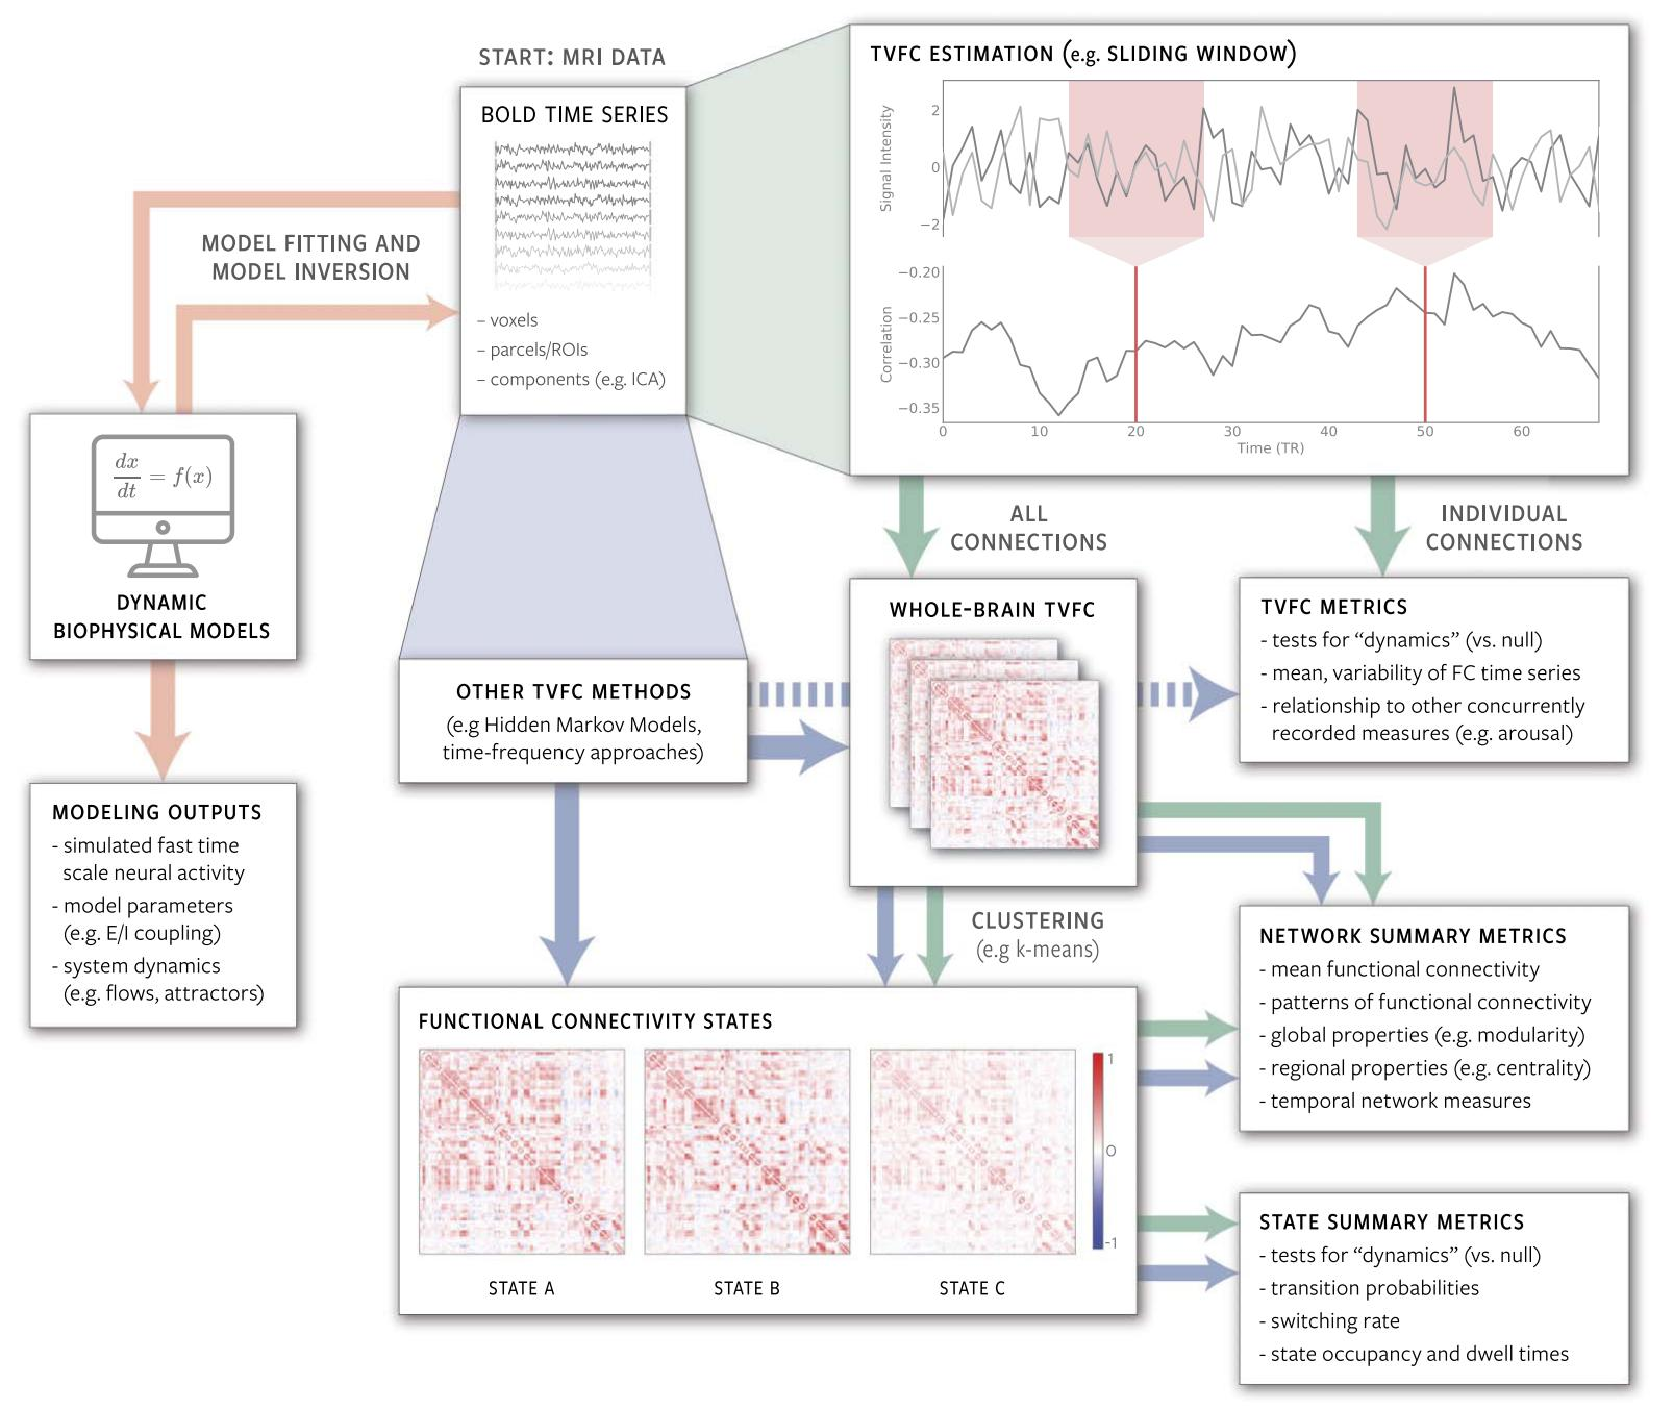
\includegraphics[width=\textwidth]{fig/tvfc_methods_Lurie2020_compressed}
  \caption{
    Typical TVFC estimation and feature extraction workflow(s) in fMRI data.
    Green arrows show a typical sliding-windows analysis, blue arrows indicate a range of other data-driven analyses, orange arrows represent fitting a biophysical model to time series data.
    Re-generated from \textcite{Lurie2020}.
  }\label{fig:tvfc-workflow}
\end{figure}


\info[inline]{Paragraph: Clear up TVFC naming convention.}
Before moving on, we need to address some housekeeping regarding naming conventions.
The terms \gls{tvfc} and \gls{dfc} (or dynFC) are sometimes used interchangeably, but sometimes refer to different things.
To avoid confusion, we will use the more general term \gls{tvfc} and a broad label, since `dynamic' functional connectivity is used in multiple ways and contexts across disciplines~\parencite[see][for more details]{Lurie2020}.

\info[inline]{Paragraph: Discuss scientific insights from TVFC.}
Although \gls{sfc} analyses have taught us a lot, \gls{tvfc} can increase our understanding of the underlying cognitive processes that generate such covariance structures~\parencite{Cohen2018}.
The study of \gls{tvfc} can help the understanding of adaptation and shifts in behavior in the brain.
%
Since \gls{tvfc} is an extension of \gls{sfc}, all information captured by \gls{sfc} should be captured by \gls{tvfc} too.
Therefore, we argue that \gls{tvfc} should always be compared to \gls{sfc} to find out what extra information is extracted from including the time-varying nature of the covariance structure.
And indeed, \gls{tvfc} has been shown to extract additional information in some cases compared to just \gls{sfc}~\parencite[see e.g.][]{Rashid2016, Jin2017, Liegeois2019, Luppi2019, Varley2020, Vidaurre2021, Coppola2022}.
These results also suggest that the study of consciousness and certain mental disorders may benefit from a dynamic view of the brain.
%
Despite these insights, there are still many open questions regarding the interpretation and validity of \gls{tvfc} estimates.
The biological and physiological basis of \gls{tvfc}, both neural and nonneural in origin, is still elusive~\parencite{Lurie2020}.
\textcite{Liu2013, Petridou2013} have suggested that \gls{tvfc} may originate from transient coactivation patterns (CAPs) and their dynamics.
\textcite{Matsui2019} later confirmed this by simultaneously recording calcium imaging and optical hemodynamics~\parencite[see][for a review of multi-modal approaches]{Thompson2018b}.
Furthermore, it has often been suggested that the brain exhibits a state-space structure, which may underlie the observed time-varying connectivity structure~\parencite{Hutchison2013}.

\info[inline]{Paragraph: Discuss open questions and limitations.}
There are ongoing debates about the physiological origins and relevance (behaviorally as well as cognitively) of \gls{tvfc}.
\textcite{Laumann2017} challenged the idea that \gls{tvfc} is related to ongoing cognition.
One potentially compelling argument against any cognitive relevance of \gls{tvfc} is that \gls{fc} fluctuations have also been observed in anesthetized (unconscious) brains~\parencite{Hutchison2013b}.
However, \textcite{Demertzi2019} found anesthesia to change network complexity, validating its implication with consciousness~\parencite[see also][]{Varley2020b}.
Furthermore, questions have been raised about the statistical validity of this construct.
As \textcite{Lurie2020} discussed, fluctuations and correlations may well be explained by nonneural physiological factors such as head motion, cardiovascular, and respiratory effects.
%
It is critical that these ambiguities are resolved before we make inferences in high-stakes settings, such as when studying mental disorders.
The work in this thesis aims to help clarify and resolve such issues.

\clearpage
\section{The trouble with estimating TVFC}
%%%%%

\info[inline]{Paragraph: Overview, scope, and importance of problem of TVFC estimation.}
One of the main reasons for the lack of understanding of \gls{tvfc} as a construct and its cognitive relevance is that the field still lacks a robust way of estimating \gls{tvfc}~\parencite{Foti2019, Lurie2020}.
Many estimation methods are used in practice, and many more have been proposed.
\gls{tvfc} estimations vary wildly across different estimation methods, and, as we will see, this results in different predictive power of subject measures (including clinical measures).
Consequently, experimental and scientific conclusions are heavily influenced by the (seemingly arbitrary) choice of estimation method.
This compounds onto the already large number of reseacher `degrees of freedom' present in \gls{fmri} analyses~\parencite{Gelman2013, Dafflon2022}.
This motivates the careful and robust development of \gls{tvfc} estimation methods.

\info[inline]{Paragraph: Introduce common estimation methods.}
Common \gls{tvfc} estimation approaches include \gls{sw} methods~\parencite{Sakoglu2010, Chang2010}, multiplication of temporal derivatives~\parencite{Shine2015}, phase coherence models~\parencite{Glerean2012}, \gls{mgarch} methods~\parencite{Lindquist2014, Choe2017, Xie2019}, a range of customized Bayesian models~\parencite[see e.g.][]{Taghia2017, Lan2017, Warnick2018, Li2019b, Ebrahimi2020}, wavelet methods~\parencite{Park2014, Zhang2016}, and phase synchronization models~\parencite{Varela2001, Glerean2012, Demirtas2016, Honari2021}.
Each of these has a range of variants and tweaks as well.
We need to be careful with comparing these approaches head-to-head, as many of these methods extract a slightly different aspect of \gls{tvfc}, where some focus more on frequency-space information, others model change points better, and some are autoregressive whereas others are not.
Moreover, it is often not clear what connectivity measure is of interest for answering a particular scientific question.
This lack of clarity is another major hurdle in the field.
%
Part of the problem is that the target audience of proposed methods differs.
Many of the more advanced model proposals address a very technical audience.
This makes practical adoption unlikely.
Additionally, such more principled and thoughtful methods are often published without clean and stable code.
These factors have led to a misalignment between thoughtful modeling experts that develop better methods and their envisioned end users, who (understandably) still often default to the simple and practical \gls{sw} approach.
%
In \cref{sec:established-methods} we will go into more technical detail on the methods considered in this thesis.
%
Although we only consider time domain methods, time-frequency parameters can still be extracted from learned model parameters, as we shall see.
Even though not every method is considered, when setting up the benchmarks it should be relatively straightforward to include another method to our comparison framework.

\info[inline]{Paragraph: Explain why method selection is hard.}
The lack of a ground truth correlation makes method selection a hard problem.
This explains why the field has not settled on a single approach.
%
In their review, \textcite{Lurie2020} noted the pitfall of studying \gls{rs-fmri} \gls{tvfc} of lacking clear benchmarks.
They also notd that \gls{rs-fmri} has already gone through similar controversies in its early days.
This invites us to learn from its respective journey as a field.

\info[inline]{Paragraph: State how we address this problem.}
How do we then determine how to estimate \gls{tvfc}?
This thesis aims to answer this question.
In short, we propose a suite of data science problems; a range of \emph{benchmarks} (see \cref{sec:benchmark-framework}).
These benchmarks are designed to capture and illuminate various estimation method attributes, strengths, and weaknesses.
Overall, the results then provide an overview of method performance and failure modes.

\clearpage
\section{Functional connectivity and depression}\label{sec:fc-depression}
%%%%%

\info[inline]{Paragraph: Introduce the general study of depression.}
In this thesis we study depression as a functional and connectivity disorder, through the lens of \gls{tvfc}.
But what do we mean by depression?
How does depression affect the brain?
And more specifically, how does depression affect \gls{fc} in the brain?
Can \gls{fc} be used to assign credit or discredit to various theories of depression?
In this thesis we argue that depression is a particularly good disease to study through the lens of \gls{tvfc}.
\gls{fc} has the potential of offering new diagnostic value in neuropsychiatric disorders, where typical \gls{fmri} activations are often small~\parencite{Fornito2012}.
The rest of this section reviews the current understanding of what depression is, why it is important to study it, what subtypes exist, what symptoms typically occur, how it affects the brain, and how it affects \gls{fc} in the brain.
Of course, this will be a limited overview of all research and perspectives on depression, but will include the most relevant background information for the study in this work.

%%
\subsection{What is depression?}\label{subsec:depression}
%%

\info[inline]{Paragraph: Overview of depression burden and motivation to study it.}
Depression is a human tragedy: it is absolutely crippling, it is pervasive, and it is global.
The most recent \gls{who} estimate (for 2021) puts the number of people worldwide living with a proverbial `black dog' at 280 million.
The burden of depression (and other neuropsychiatric disorders) on societies and their healthcare systems barely needs elaboration.
Even more worrisome is that its disease burden and prevalence are growing.
Stigma, heterogeneity of symptoms, and lack of understanding of causes and brain and social mechanisms have meant that treatment of this disorder (or umbrella of disorders) remains insufficient.
Depression is slightly different for everyone and remains difficult to conceptualize.
We may call it a disease, illness, or disorder, but we may also view it as an \emph{experience} instead.

\info[inline]{Paragraph: Introduce depressive disorders and describe MDD.}
This thesis is mainly concerned with \gls{mdd}, the most common of all depressive disorders.
It is important to distinguish between three types of depression: the everyday, colloquial use of the word depression; a longer period of sadness after a traumatic life event (a \emph{reactive} depression); and \textbf{major depression}, which is characterized by \emph{persistent} sadness over prolonged periods of time~\parencite{Otte2016}.
Going forward we refer to the latter when we talk about depression.
Two common ways of diagnosing (i.e.~categorizing or classifying) depression are based on standard diagnostic (category-based) frameworks: the \gls{dsm} and the \gls{icd}.\footnote{The \gls{icd} defines mental disorders as ``clinically recognizable set of symptoms or behaviors associated in most cases with distress and with interference with personal functions''~\parencite{WHO1992}.}
The \gls{dsm} criteria for major depression are shown in Box~\ref{box:depression}.
We shall return to these criteria in \cref{subsec:cohort-stratification} for defining participant cohorts.
The \gls{icd} criteria are similar, requiring three criteria to be met: persistent low mood or loss of interests; happening for most of the time on most days for at least two weeks; and experiencing four or more other symptoms like disturbed sleep, concentration, appetite, guilt, self-blame, low self-esteem, agitation, and/or suicidal thoughts.
More broadly, depression endophenotypes\footnote{Endophenotypes, or `intermediate phenotypes', refer to heritable traits used to more robustly define behavioral symptoms into phenotypes. Similar terms are `biological marker' or \emph{biomarker} and `subclinical trait', although these are typically not used to refer to genetic components.} and cardinal symptoms include anhedonia, anergia, anxiety, rumination, changes in appetite and sleep patterns, strong and persistent feelings of guilt and grief, and, most tragically, self-injury~\parencite{Goldstein2014, Pizzagalli2014}.
Although core symptoms are typically present, depression is not a consistent syndrome with a fixed set of symptoms.
In fact, \textcite{Fried2015} found over 1,000 unique symptoms in a cohort of about 3,700 patients~\parencite[see also][]{Fried2015b}.
\Gls{mdd} not only affects mood and affective processing but is also involved with a range of cognitive dysfunctions.

\begin{mybox}[floatplacement=t,fontupper=\footnotesize,fontlower=\footnotesize,label={box:depression},colback=White]{Depression and its symptoms}

  The latest version of the \gls{dsm} (version 5, released by the American Psychiatric Association in 2013) outlines the following symptoms and criteria for diagnosing \gls{mdd}.
  The individual at hand must experience five or more of the following symptoms, persisting for at least two weeks.
  Symptoms must be present nearly every day, for most of the day.
  One of the two `core' symptoms, depressed mood (1) or (2) loss of interest or pleasure, must be present.

  \tcblower

  \begin{enumerate}
    \item Depressed, sad, and/or low mood.
    \item Diminished interest or pleasure in all, or almost all, activities.
    \item Significant weight loss or weight gain, or changes in appetite.
    \item Sleeping too much, too little, or not well (insomnia).
    \item A slowing down of thought and a reduction of physical movement (observable by others, not merely subjective feelings of restlessness or being slowed down), that is psychomotor agitation or retardation.
    \item Fatigue or loss of energy.
    \item Feelings of worthlessness or excessive or inappropriate guilt.
    \item Diminished ability to think or concentrate, or indecisiveness.
    \item Recurrent thoughts of death, suicidal ideation (with or without a specific plan), or a suicide attempt.
  \end{enumerate}

\end{mybox}

\info[inline]{Paragraph: Discuss causes and enviromental factors for depressive disorders.}
What causes depression?
As there are various subtypes of depression, this varies.
However, commonly depressive episodes are predated by traumatic, adverse, and negative life events~\parencite{Kessler1997, Monroe2008}.
When such events happen at a developmental age, they can disproportionally impact neurobiological systems, and lead to a higher probability of developing depression later in life.
Perhaps the right question is not what causes depressive episodes, but what makes some individuals more \emph{resilient} in the face of stressors to be able to cope and recover.
As such it is common to talk about `risk' or `contributing' factors (such as genetics, early life experiences, socioeconomic status, and environment), instead of `causes'.
Most prevention efforts would focus on managing exactly these contributing factors.

\info[inline]{Paragraph: Discuss genetic contribution to MDD.}
There is some evidence for a genetic basis or predisposition to depression.
This will be relevant in \cref{subsec:cohort-stratification}.
We know that \gls{mdd} has a heritable component.
Genetic risk for \gls{mdd} is polygenic, meaning a variety of genes are involved, and the exact mechanisms are yet to be uncovered~\parencite{Hyman2014}.
This is likely due to the heterogeneity of depressive symptoms as well.
Moreover, much of depression risk may be due to other genetic factors.
Higher overall cognitive function, for example, could lead to higher socioeconomic status, which in turn could lead to a healthier diet and an increased sense of safety and control in the world (which in turn have been linked to lower depression risk).
Genetic risk has often been described as influencing cognitive biases and thus \emph{resilience} to stressors.
The most important take-away from genetic studies is that genes are about vulnerability and resilience to depression and not about inevitability.
%
In a large cohort study, \textcite{Garcia-Gonzalez2017} failed to find a robust genetic contribution to treatment response.

\info[inline]{Paragraph: Describe cognitive effects of MDD.}
Before looking at the brain and the impacts of \gls{mdd} on \gls{fc}, we give an overview of changes in cognition and behavior.
These will be referred to in \cref{sec:ukb-discussion}.
Deficits in memory systems, attention, learning, processing speed, and decision-making are common among \gls{mdd} patients.
\textcite{Rock2014} found especially executive function\footnote{In neuroscience, \textbf{executive function} generally refers to functions related to planning, focus, sticking with instructions, and multi-tasking~\parencite{Banich2009}.}, memory, and attention affected by \gls{mdd}.
Dysfunction is linked to a range of cognitive and affective biases.
A core affective bias is toward paying attention to the negative, or only remembering the negative~\parencite{Pulcu2017}.
For example, depressed individuals forget negative information at a slower rate~\parencite{Power2000, Joormann2010}.

\info[inline]{Paragraph: Discuss integrated models of depression.}
Key to all of this is to find ways to \emph{integrate} or \emph{unify} the various perspectives on depression.
Several proposals have been made to build integrated models of depression.
Most of these agree that we need a bridge between the psychological perspective (the one that `makes sense' but we cannot do modern science on) and the biological perspective (the one that we can measure and work with but is often too far removed from the human experience).
\textcite{Akiskal1973} discussed ways to integrate such psychological and biological views of depression.
Their proposed framework integrates several depression characterizations; metapsychological (Freud's ``aggression-turned-inwards'' and the ``object-loss'' models), the ``reinforcement'' model, and the biological (``biogenic amine'') model into a common pathway of ``functional derangement of the mechanisms of reinforcement''.
\textcite{Pizzagalli2014} proposed that anhedonia is the key feature of depression, and proposes an account of anhedonia, \gls{da} (reward systems), and the (internal) massive stress responses and heightened stress hormone levels found in depressed patients.
More recently, \textcite{Beck2016} proposed that depression can be viewed as ``an adaptation to conserve energy after the \emph{perceived loss of an investment in a vital resource} such as a relationship, group identity, or personal asset.''
They highlight that these are mediated by brain regions involved in cognition and emotion regulation: the \gls{amg}, \gls{hpc}, and \gls{pfc}.
According to this proposal, depression can be viewed as an ``evolutionary program'' for conserving energy, that just so happens to have become maladaptive in contemporary life.\footnote{Other maladies can also be attributed to such unfortunate evolutionary left-overs. Instinctive hoarding of sugar and information had evolutionary advantages, but wreaks havoc in modern life.}
Overall, many of these existing grand theories share a lot of common ground.
Most descriptions gear toward perturbations in reinforcement processing, negative affective bias~\parencite{Pulcu2017}, negative feedback loops, stress, and associated neurochemical pathways.
However, at the time of writing most of these are still quite general and fail to make concrete, falsifiable predictions, crucial for the development of strong theory.
It also remains to be seen whether a single model will be able to describe all clinical cases.

\info[inline]{Paragraph: Discuss treatment options for MDD.}
That brings us to the treatment of depression.
Importantly, knowing what works to treat depression and what does not can also shed light on what the condition entails.
Treatment options for \gls{mdd} generally are pharmacological intervention and/or one of the many types of (psycho)therapy~\parencite{Otte2016}.
Antidepressant medication is usually meant to increase the concentration of a certain neurotransmitter in the brain, most commonly serotonin.
In the case of serotonin, these antidepressants are called \gls{ssri}.
Interest in therapies using psilocybin~\parencite{Carhart-Harris2016, Luppi2021, Daws2022, Singleton2022} and ketamine~\parencite{Krystal2019, Kotoula2021} has spiked in recent years as well, but the jury is still out on the efficacy of such treatments.
Depression is seen as decreasing brain state entropy, which psychedelics can alleviate, as it lies on the opposite side of a spatiotemporal dynamics spectrum~\parencite{Vohryzek2022}.
%
There is an intense debate in society at large on how best to treat depression, some pointing predominantly to medication, and others to social approaches.
Part of this controversy stems from the fact that depression is still poorly understood, and it is likely grouping together many types of depression.
For example, medication seems to work well for some but has no effect on others.
The latter are sometimes called `treatment-resistant', but they may well suffer from a different subtype of depression, where neurobiologically distinct domains are collapsed into a simple diagnostic index.
Overall, there are many things that can help those with depression.
However, one of the crucial issues is that not all these things help everyone, and matching the right support to the right person is hard.
Each patient is characterized by a unique mixture of medical history, personality, comorbidities, socioeconomic environment, and many other factors~\parencite{Trivedi2006}.
Here lies the challenge of the treatment of depression in society: how do we provide care with the required level of personalization, yet to millions of people at the same time?

%%
\subsection{Depression and neuroimaging}\label{subsec:fc-neuroimaging}
%%

Neuroimaging has the potential to offer unique insight into the mechanisms of depression.
A lot of neuroimaging can be considered a mapping exercise.
Starting from how the brain is anatomically characterized, to mapping literal wiring diagrams such as white matter tracts, but also including the \gls{fc} mapping exercise as we study here.
Once we have a good map, it is natural to ask whether we can find individual landmarks that are unique to a disease.

Structural scans have shown that the neuroanatomy in depressed patients is affected~\parencite{Drevets2000}.
Multiple brain region volumes are either increased or decreased~\parencite{Sacher2012, Schmaal2020}.
Grey matter volumes are \emph{reduced} in the \gls{amg}, \gls{pccx}, \gls{dmpfc}, and \gls{hpc}.
However, there are conflicting findings, and \gls{amg} volume may be increased or decreased based on individual specifics.
Volumetric increases have been reported for the insula, middle frontal gyrus, superior frontal gyrus, and the thalamus.\footnote{In neuroanatomy, a \textbf{gyrus} refers to the ridges of the cortex surface, opposed to a \textbf{sulcus}, which refers to the respective furrow of the folded cortex.}

However, recent meta-analyses have come to dispute the reliability and clinical relevance of many such findings.
A recent large (1809 participants) study found very modest predictive power of (univariate) neuroimaging modalities (\gls{mri}, \gls{dti}, \gls{rs-fmri}, and \gls{tb-fmri}) of \gls{mdd}~\parencite{Winter2022}.
They found environmental factors such as social support and childhood maltreatment to have much more predictive power.
Similar sentiments were echoed in \textcite{Nour2022}.
At present, neuroimaging plays little to no role in clinical decision-making~\parencite{Kapur2012}.

%%
\subsection{Functional connectivity in psychiatric disorders}\label{subsec:fc-depression}
%%

\info[inline]{Paragraph: How can we relate functional connectivity to disorders? What can this teach us about these disorders? What value do these analyses have in a clinical setting?}
Whereas some brain disorders and mental health conditions can be traced back to a dysfunction in a particular brain region (e.g.~inflammation, neurodegeneration,\footnote{Neurodegenerative disorders refer to progressive loss of neural structure and function. Common disorders in this category include \gls{ad} and \gls{pd}.} or physical trauma), others are better understood as dysfunction in brain region \emph{function} and/or \emph{interaction} between otherwise seemingly healthy individual brain regions.
Mood disorders\footnote{In psychiatry, a \textbf{mood} or \textbf{affective disorder} refers to any depressive or bipolar disorder.} especially have been suggested to be functional (related to dynamic connectivity patterns) rather than structural disorders~\parencite{Piguet2021}.
\Gls{fc} is a particularly useful framework to study such aberrations in connectivity with, witnessed by the vast number of studies studying depression through this lens.

\info[inline]{Paragraph: Discuss sFC in neurological and psychiatric disorders.}
Most of such psychiatric studies employ \gls{sfc}.
These estimates have demonstrated potential and promise to be used in clinical settings~\parencite{Cole2014, Deco2014, Parkes2020}, or at least have some predictive power.
For example, it has been shown to be useful as biomarkers for depression~\parencite{Drysdale2017}.
The promise of using connectomics for understanding neuropsychiatric disorders has been expressed many times~\parencite{Deco2014}, and many \gls{sfc} studies have been conducted.
Building on top of advances in network neuroscience has shown more potential for clinical discovery from \gls{fc}~\parencite{Lydon-Staley2018}, where network features can be used as biomarkers of disease~\parencite{Bassett2009}.
Another data point that highlights the promise of studying \gls{mdd} through the perspective of \gls{fc} is that such connectivity and networks have been found to re-normalize after anti-depressants treatment.

\info[inline]{Paragraph: Discuss FNs in neurological and psychiatric disorders.}
\Glspl{fn} are often affected by neuropsychiatric disorders, even if their individual brain region constituents appear normal.
Such disorders are therefore increasingly studied as \emph{network} disorders~\parencite[see][for a review on depression]{Mulders2015}.
Instead of a single brain region not functioning properly, there is an aberration in the integration and segregation of brain regions.
These changes in \gls{fn} are believed to contribute to or be caused by cognitive changes from mental illness.
Many mental illness conditions have been postulated to occur with large-scale disruptions, driven by neurotransmitter dysfunction, of whole-brain systems.
Even though whole-brain \glspl{fn} are found to be highly similar across groups with or without a range of mental illnesses, the subtle differences that \emph{do} occur are meaningful in the sense that they are predictive of diagnosis~\parencite{Spronk2020}.
This makes intuitive sense as well: a piano does not need major disruption to ruin a classical piece, one key being out of tune is sufficient~\parencite[see also][for a discussion of small effect sizes]{Paulus2019}.
Perhaps this is even encouraging.
If small network alterations can result in mental disease, a small intervention can bring someone's functional architecture back on track.

\textcite{Mulders2015} found the main networks to be involved and affected in depression to be the \gls{dmn}~\parencite{Berman2011, Demirtas2016, Wise2017, Yan2019, Zhao2019, Zhou2020}, \gls{cen}~\parencite{Zhao2019}, and \gls{sn}~\parencite{Manoliu2014}.
These are also generally the networks most studied and will be the ones considered in this thesis.
The exact makeup of these networks varies across studies.
A rough overview of each network is provided here (the more precise implementational details will be provided in \cref{subsec:ukb-fn-analysis}).

The \gls{dmn} primarily consists of the \gls{mpfc} and \gls{pcc}, as well as the (para)hippocampal areas, precuneus (cortex), and angular gyrus~\parencite{Andrews-Hanna2010}.
It is often described as the neurological basis for `the self' and is attributed to functions like self-referential thinking~\parencite{Sheline2009}, cognitive flexibility~\parencite{Vatansever2016}, mind-wandering, memory processing and rumination, theory of mind, emotion regulation, and as storage of autobiographical information.
It is connected to the \gls{amg} and \gls{hpc}~\parencite{Andrews-Hanna2014}.

The \gls{cen} primarily consists of the lateral \gls{pfc}, posterior parietal cortex (PPC), \gls{dlpfc} (especially middle frontal gyrus), \gls{dmpfc}, and posterior parietal regions~\parencite{Rogers2004}.
It is associated with cognitive processes and functions, like working memory and attention.

The \gls{sn} primarily consists of the \gls{ai} and (dorsal) \gls{acc}, with some adding the \gls{amg}, frontoinsular cortex, temporal poles, and striatum~\parencite{Seeley2007, Menon2010, Beck2016}.
The \gls{sn} is a key network in cognitive flexibility~\parencite{Dajani2015}.

\info[inline]{Paragraph: Discuss TVFC in neurological and psychiatric disorders.}
What about the dynamics of \gls{fc}?
The promise of \gls{tvfc} has been highlighted more recently as well in neurodegenerative conditions~\parencite{Filippi2019}.
More relevant information is contained in \gls{tvfc} compared to \gls{sfc}.
\gls{tvfc} may be especially relevant for dynamic brain disorders like schizophrenia~\parencite{Jin2017}.

\info[inline]{Paragraph: Discuss graph topology in neurological and psychiatric disorders.}
Graph topology and network neuroscience have also been suggested to shed more light on neurological and psychiatric conditions~\parencite{Fornito2013}.
Connectomic graph theoretic approaches to depression have found smaller path lengths and higher global efficiency~\parencite{Zhang2011}.
This has been interpreted as a shift toward brain network randomization~\parencite{Gong2015}.

\clearpage
\section{Outline and contributions of thesis}
%%%%%

\info[inline]{Paragraph: Overview methods development.}
In this thesis we propose a novel method, the \gls{wp}, to estimate \gls{tvfc} in a more principled and robust way.
Similar in spirit to the \gls{gp}, these models learn a distribution over (covariance) matrix-valued functions (where \glspl{gp} learn a distribution over scalar-valued functions).
This class of models has become a practical possibility in neuroimaging recently, due to advancements in approximate inference routines~\parencite{Heaukulani2019} and easy-to-use computational libraries~\parencite{Matthews2017}.
To address the practical difficulty of estimating \gls{tvfc}, we release all models and software into an open-source code repository.
We welcome researchers and practitioners to provide feedback or to add other estimation methods to this repository.

\info[inline]{Paragraph: Overview benchmarking.}
Furthermore, we propose an extensive benchmarking framework to compare \gls{tvfc} estimation methods.
We compare our new method to baseline approaches, such as an improved version of the \gls{sw} approach and \gls{mgarch} models.
We discuss desired qualitative properties of \gls{tvfc} estimation methods and how they may influence which method to use.

\info[inline]{Paragraph: Overview depression study.}
Lastly, we apply this robust method (the `winner' of the benchmarking efforts) in a large, exploratory clinical study, seeking to contrast depressed and healthy individuals.
Multiple depression phenotypes and \gls{tvfc} metrics are studied to provide a rich multiverse of scientific insight.

\info[inline]{Paragraph: Provide thesis outline.}
In \cref{ch:methods} we go through established \gls{tvfc} estimation methods, our novel approach, as well as the benchmarking framework used to compare estimation methods.
The remaining (experimental) chapters are about applying these methods.
They are structured in ascending order of complexity and practicality, starting with simple, synthetic data sets to real, large-sample resting-state and task-based \gls{fmri} data in \cref{ch:benchmarking}, to the application in a large population study in \cref{ch:ukb}.
In \cref{ch:discussion} we review and interpret our results and set out directions for future work.

\info[inline]{Paragraph: Final comments before wrapping up the introduction.}
We hope this thesis and accompanying software package can help researchers make more robust \gls{tvfc} brain connectivity estimates and shed more light on what we can infer from this construct.
Moreover, we hope it contributes to the understanding of how depression is related to the (dynamic) functional architecture of the human brain.
%
As we are in an interdisciplinary field, we have aimed for this thesis to be readable for as broad of an audience as (reasonably) possible, from psychologists to neuroscientists to machine learning experts to clinicians and beyond.
This means, for example, that we have taken special care in aligning jargon across these disciplines.

%%
\chapter{Robust estimation of TVFC}\label{ch:methods}
%%%%%

\info[inline]{Paragraph: Overview of chapter.}
In this chapter we frame and define the problem of \gls{tvfc} estimation.
We describe key established methods for this task and the development of new ones; the \gls{wp} in particular.
Additionally, we motivate the importance and describe several ways of extracting features or \emph{(bio)markers} from \gls{tvfc}.
These will be used in further analyses in the following chapters.
%
Furthermore, we discuss how to compare and evaluate these methods, to weigh which one we ought to use.
Our aim is to develop \emph{robust} \gls{tvfc} estimation methods.
Above all, we need to convince \emph{ourselves} that any method we opt to use is valid.
In the words of the legendary physicist Richard~Feynman: ``The first principle is that you must not fool yourself, and you are the easiest person to fool''.
%
This chapter closes with a brief discussion on the nature of estimation methods.

\info[inline]{Paragraph: Frame TVFC estimation as covariance structure estimation problem.}
The estimation of \gls{tvfc} (as we have narrowly defined it in the introduction to this thesis) is a particular form of the more general problem of covariance structure estimation.
This problem has been of interest to statisticians and computer scientists for a long time.
It has been studied extensively in the machine learning and econometrics (e.g.~modern portfolio theory) communities.
%
However, each application domain has its own unique characteristics.
Directly copying approaches and methods is not sufficient.
For example, those who study financial markets are mostly interested in using covariance structure modeling to estimate \emph{future} events and returns.
Neuroscientists typically are not interested in such forecasting.

\info[inline]{Paragraph: Introduce concept of covariance.}
To recap, the \textbf{covariance} between two random variables $X$ and $Y$ is defined as the expected value of the product of the deviations of these variables from their individual expected values (i.e.~means):
\begin{equation}
  \begin{aligned}
    \sigma_{xy} & = \mathbb{E}[(X - \mathbb{E}[X])(Y - \mathbb{E}[Y])] \\ & = \mathbb{E}[XY] - \mathbb{E}[X]\mathbb{E}[Y].
  \end{aligned}
  \label{eq:covariance}
\end{equation}
It is a \emph{linear} measure of joint variability of random variables.
A \textbf{covariance matrix} ($D = 2$ dimensional in this case; a.k.a.~variance matrices) collects all such covariances and is defined as
\begin{equation}
  \mathbf{\Sigma} = \begin{bmatrix}
    \sigma_x^2  & \sigma_{xy} \\
    \sigma_{xy} & \sigma_y^2
  \end{bmatrix},
\end{equation}
where~$\sigma_x^2$ and~$\sigma_y^2$ are the respective \textbf{variances} of the random variables, and $\sigma_x$ and $\sigma_y$ are called the respective \textbf{standard deviations}.
Covariance matrices are required to be symmetric (i.e.~$\mathbf{\Sigma} = \mathbf{\Sigma}^T$) and positive semi-definite (having only positive eigenvalues, i.e.~$\mathbf{v}^T \mathbf{\Sigma} \mathbf{v} \geq 0$ for all vectors $\mathbf{v} \in \mathbb{R}^D$).
The converse is true as well; every symmetric, positive semi-definite matrix is a covariance matrix.
The inverse of a covariance matrix $\mathbf{\Sigma}^{-1}$ is called a precision matrix.

\info[inline]{Paragraph: Introduce concept of Pearson correlation.}
As discussed previously, in the study of \gls{fc} it is more common to use Pearson correlation coefficients instead of covariance.
These are \emph{dimensionless} measures of linear dependence.
They can be understood as a normalized version of covariance.
As such, they are more interpretable and easier to work with.
Correlation values are bound to range~$[-1,1]$, where a correlation of~1~indicates perfect correlation (i.e.~it is possible to draw a straight line that perfectly fits all data),~-1~indicates perfect anti-correlation, and~0~indicates uncorrelation (which does \emph{not} imply independence).
The Pearson correlation coefficient can be interpreted as a measure of how well the optimal linear function describing the random variable relationship fits the data.
A (Pearson) \textbf{correlation matrix} is defined as
\begin{equation}
  \label{eq:correlation-matrix}
  \mathbf{\Sigma} = \begin{bmatrix}
    1 & \frac{\sigma_{xy}}{\sigma_x\sigma_y} \\
    \frac{\sigma_{xy}}{\sigma_x\sigma_y} & 1
  \end{bmatrix}.
\end{equation}
If all random variables considered have standard deviation (and variance) equal to~1, the covariance and correlation matrix are identical.\footnote{In fact, this is often the case, as normalizing time series variance is common practice in \gls{fc} studies~\parencite[see e.g.][]{Beckmann2004, Allen2014}.}
Throughout this thesis, \gls{fc} refers to this correlation metric.
All plots will show correlation estimates instead of covariance estimates.
%
We will refer to a single \gls{fc} correlation matrix as a connectivity \emph{state}, and refer to this correlation matrix as a function of time (i.e.~\gls{tvfc}) as covariance or correlation \emph{structure} (used interchangeably).
%
On a cautionary note, using the Pearson correlation as connectivity measure may be too simple.
It assumes that time series are homoscedastic, meaning the variance across a brain scan is homogenous.
Furthermore, this measure is known to be heavily skewed by outliers.
It also does not make any claims of \emph{directionality}.

\info[inline]{Paragraph: Outline of this chapter.}
The rest of this chapter is organized as follows.
Firstly, we discuss established and commonly used \gls{tvfc} estimation methods in the field, and our particular implementation of them.
Then, we discuss how to run the \gls{sw} method in a principled and improved way using cross-validation.
Afterwards, we discuss a proposed new method for estimating \gls{tvfc}: the \gls{wp}.
Then, we discuss how a range of features~\parencite[or \emph{biomarkers} as they are often called in the context of neuroimaging, see e.g.][]{Woo2017, Douw2022} can be extracted from such estimated \gls{tvfc} and the estimation methods discussed.
%
Finally, we discuss a framework of benchmarks by which we can robustly assess and compare method performance.
%
We quickly discuss key methodological issues and controversies before moving on to the empirical studies.

\clearpage
\section{Established methods and baselines}\label{sec:established-methods}
%%%%%
\info[inline]{Section: Introduce key and established TVFC estimation methods.}

In this section we briefly describe established, state-of-the-art, and popular \gls{tvfc} estimation methods in the field.
Only methods that are used as baseline methods for comparison in our benchmarks and experiments are discussed in more detail.

%%
\subsection{Static functional connectivity}
%%

\info[inline]{Paragraph: Introduce static functional connectivity estimation.}
Any proposed \gls{tvfc} estimation method has to be compared with a \emph{static} (time-invariant) analysis.
The \gls{sfc} approach makes the implicit assumption that the covariance between random variables of interest (e.g.~brain region time series) does not change across time (i.e.~any arbitrary length of scanning session).
Statistically, it assumes that node time series are \emph{stationary}, and thus that connectivity can be considered a \emph{global} property.
This approach extracts the \emph{general} functional architecture of a particular subject, instead of the moment-to-moment functional interactions.
%
The inclusion of \gls{sfc} in any analysis serves as a sanity check.
The mean of \gls{tvfc} estimates should be similar to the \gls{sfc} estimate.
Furthermore, if a \gls{tvfc} estimation method cannot outperform the \gls{sfc} estimate on some task, this may either indicate that there is no (relevant) dynamic signal in the data set, or that the estimation method is flawed.

\info[inline]{Paragraph: Describe our static functional connectivity estimation.}
A standard covariance \gls{sfc} approach simply computes the covariance between node time series (i.e.~regional activity) across the entire brain scan duration as in \cref{eq:covariance}:
\begin{equation}
  \begin{aligned}
    \sigma_{ij} & = \mathbb{E}[(y_i - \mathbb{E}[y_i])(y_j - \mathbb{E}[y_j])] \\ & = \frac{1}{N} \sum_{n=1}^N (y_{i,n} - \bar y_i)(y_{j,n} - \bar y_j),
  \end{aligned}
\end{equation}
where $\sigma_{ij}$ is the covariance between variables $y_i$ and $y_j$ (two different brain region \gls{bold} time series) for their $N$ observations in the entire time series, for $1 \leq i \leq D$ and $1 \leq j \leq D$.
The respective Pearson correlation coefficient is then given by
\begin{equation}
  \label{eq:sfc-estimation}
  \rho_{ij} = \frac{\sigma_{ij}}{\frac{1}{N} \sqrt{\sum_{n=1}^N (y_{i,n} - \bar y_i)^2 \sum_{n=1}^N (y_{j,n} - \bar y_j)^2}}.
\end{equation}
When $D > 2$, the full estimated correlation matrix can be estimated by looping over all edges in pairwise fashion.
Although \gls{sfc} estimates in neuroimaging are typically computed as described here, there are many other versions available, for example using sparsity-inducing penalties~\parencite{Foti2019}.
%
Since we assume (or enforce) all $\bar y_i$ to be zero, perhaps the simplest connectivity estimate is the covariance matrix \gls{mle}:
\begin{equation}
  \hat{\mathbf{\Sigma}}^{MLE} = \frac{1}{N} \sum_{n=1}^N \mathbf{y}_{n} \mathbf{y}_{n}^T.
\end{equation}
However, in this work we use the unbiased estimator instead:
\begin{equation}
  \hat{\mathbf{\Sigma}} = \frac{1}{N - 1} \sum_{n=1}^N \mathbf{y}_{n} \mathbf{y}_{n}^T.
\end{equation}
For larger values of $N$ this difference becomes negligible.

%%
\subsection{Sliding-windows functional connectivity}\label{subsec:sliding-windows-fc}
%%

\info[inline]{Paragraph: Introduce sliding-windows functional connectivity estimation.}
Albeit criticism, \gls{tvfc} estimation methods based on \gls{sw}~\parencite{Chang2010, Sakoglu2010, Allen2014, Shakil2016, Preti2017} are still the most used throughout the neuroscience literature~\parencite{Lurie2020}.
%
This approach slides (or \emph{rolls}) a time window of a certain size (length)~$w$ and shape (e.g.~square, Gaussian) across the observations (typically with a step size of a single volume), and estimates the covariance or correlation as for the \gls{sfc} case in \cref{eq:sfc-estimation} for each step.
As such it can be considered a (weighted) moving average.
The benefits of using \gls{sw} include that it is well-established, computationally cheap, and simple to implement.

\info[inline]{Paragraph: Discuss variations on sliding-windows functional connectivity.}
Many variations of this method exist and how to best implement \gls{sw} methods has been studied extensively~\parencite[see e.g.][]{Mokhtari2019, Vergara2019}.
One popular way to reduce sensitivity to outliers is \emph{tapered} \gls{sw}.
This approach assigns less weight to observations further away from the center of the window~\parencite{Allen2014, Lindquist2014}.
Effectively this just changes the shape of the window from rectangular/square into e.g.~a Gaussian curve.
%
Rules of thumb have been established regarding window length~$w$ and necessary data preprocessing steps.
%
The lack of consistency across studies in the implementation of \gls{sw} is sub-optimal as it makes comparison across studies harder.
Furthermore, stacking heuristics does not scale.
Typically, this situation is when we should start applying machine learning techniques~\parencite[][built this case beautifully]{Zinkevich2015}.

\info[inline]{Paragraph: Discuss problems with sliding-windows functional connectivity.}
The main problem with this method is that without knowing the underlying process (i.e.~covariance structure from brain dynamics), it is hard to pick the right window length.
%
The \gls{sw} approach is also not a \emph{model-based}~\parencite{Foti2019} or \emph{data-driven} approach.\footnote{In neuroscientific context, `data-driven' refers to extracting insights directly from data in a relatively unbiased manner. It is often juxtaposed to `hypothesis-driven' or `theory-driven'.}
Furthermore, the desired behavior at the start and end of the time series is not clear.
See \textcite{Lindquist2014, Leonardi2015, Hindriks2016} for more important nuances and pitfalls of \gls{sw} methods.

\info[inline]{Paragraph: Discuss our particular implementation.}
In all experiments and benchmarks that follow in this thesis we implement a standard \gls{sw} approach to mimic a typical (often non-technical) investigator interested in using the construct of \gls{tvfc} to study the brain.
Researchers are recommended to use a window length of between 30 and 60 seconds~\parencite{Shirer2012}.
Both of these window lengths are implemented to test the limit cases.
We implement the rectangular (non-tapered) window, with a step size of a single volume.
We follow the rule of thumb proposed by \textcite{Leonardi2015} and high-pass filter the data to remove frequency components below $\frac{1}{w}$ before running the \gls{sw} algorithm.\footnote{\textcite{Smith2012} and \textcite{Hutchison2013} made similar suggestions.}
Zeros are padded to the start and end of the node time series to allow for computing the correlation coefficients around those locations.

%%
\subsection{Multivariate GARCH}
%%

\info[inline]{Paragraph: Introduce MGARCH.}
A commonly used and in many applications unsurpassed algorithm for modeling time-varying covariance structures is the multivariate version of the \gls{garch}~\parencite{Engle1982, Bollerslev1986} process.
This class of methods was first described and used in econometrics.\footnote{In this field they are commonly referred to as multivariate volatility models. In fact, methods for analyzing economic time series with time-varying volatility are deemed so important that Robert Engle and Clive Granger won the 2003 Nobel prize for their contribution to their development.}
Work on \gls{mgarch} models is still primarily motivated by financial applications.
In such contexts, the prediction task at hand is typically to forecast the next value(s).
This may not typically be the case for neuroscientists (see also \cref{subsec:imputation-benchmark}).
%
\textcite{Lindquist2014} introduced this method for estimating \gls{tvfc}, and it has been used in many studies since~\parencite[see e.g.][]{Choe2017, Preti2017, Foti2019, Hakimdavoodi2020}.
Factored models using low-rank decompositions to deal with high dimensions have been applied to \gls{eeg} sensor data~\parencite{Nakajima2017}.
We discuss similarly factored models for the \gls{wp} in \cref{subsec:model-extensions}.
%
In their early model comparison study, \textcite{Lindquist2014} showed that this method outperforms a naive \gls{sw} approach in many ways (even after post-hoc selection of the optimal fixed window length).
It should not come as a surprise then that methods based on \gls{sw} are not used in finance.
%
A commonly cited reason for the use of \gls{mgarch} in modelling financial time series is that they contain a lot of noise, requiring the use of stochastic methods.
Neuroimaging time series share these data characteristics.

\info[inline]{Paragraph: Describe MGARCH algorithm.}
Many versions and implementations of \gls{mgarch} models exist, as they describe a general \emph{family} of models~\parencite[see][for an extensive overview]{Silvennoinen2009}.
%
The general \gls{mgarch} framework considers a zero-mean vector stochastic process $\mathbf{y}_n \in \mathbb{R}^D$ with time-varying covariance structure $\mathbf{\Sigma}_n$:
\begin{equation}
  \mathbf{y}_n = \mathbf{\Sigma}_n^{\frac12} \mathbf{\eta}_n,
\end{equation}
where $\mathbf{\eta}_n$ is an i.i.d. white noise vector process.
As this is an autoregressive process, $\mathbf{\Sigma}_n$ is only conditioned on all observations up until time $n - 1$.
It assumes that the variances of the individual node time series follow a vector autoregression (VAR) process.
%
Our job as the modeler is then to model $\mathbf{\Sigma}_n$, for which several options exist.
In this thesis, we only consider and report the \gls{dcc} model.
With its introduction, \textcite{Engle2002} showed it to outperform other \gls{mgarch} variants.
It is by far the most common variant used in \gls{rs-fmri} analyses, which allows for better comparison.
Furthermore, \textcite{Heaukulani2019} found the \gls{dcc} variant to outperform the generalized orthogonal~(GO) \gls{garch} model, which is another popular \gls{mgarch} variant.
This latter variant was implemented at an early stage of this work but was consistently outperformed by \gls{dcc} and less robust in its implementation.

\info[inline]{Paragraph: Describe DCC implementation.}
More specifically, throughout this thesis, we implement DCC(1,1)-GARCH(1,1) using the open-source \texttt{R} (version 4.1.0) package \texttt{rmgarch}~\parencite{Galanos2022}.
One of the benefits of this method is that it is well understood and that convenient off-the-shelf implementations exist.
\Gls{mgarch} has several free parameters, although these are often hard to interpret and scale with data dimension to the fourth power~\parencite{Silvennoinen2009}.
\Gls{mgarch} models are known to scale poorly to higher dimensions, although workarounds have been proposed~\parencite[see e.g.][]{Nakajima2017}.
Therefore, \textcite{Gourieroux2009} claimed that these models are typically limited to studying $D < 6$ components.

%%
\subsection{State-based models}\label{subsec:state-based-models}
%%

For completeness, we briefly review state-based models.
These models are sometimes referred to as \emph{switching} models.
They assume a state-space structure of brain activity, consisting of recurring \gls{fc} patterns (see \cref{subsec:brain-states} for more details on this brain state construct).
Brain region dependencies only change when switching brain states.
If such an assumption is made, it makes sense to incorporate this in a model.

The dominant model used for this is the \gls{hmm}~\parencite[see e.g.][]{Vidaurre2017, Ahrends2022}.
It assumes the brain state stochastic process (often called a \emph{chain} in this context) to model is Markovian, meaning the probability of finding oneself in each state in the sequence of all states only depends on the previous state.
However, these states are modeled as `hidden' (i.e.~latent).
The observable process $\mathbf{y}_n$, the \gls{bold} node time series, is then used to infer the underlying hidden brain state process.

\clearpage
\section{Cross-validated sliding-windows}\label{sec:cross-validated-sw}
%%%%%

\info[inline]{Paragraph: Discuss other proposals for determining the optimal window length.}
Attempts have been made to improve \gls{sw} estimates by automatically extracting the optimal window length for a given scan from the data itself or to circumvent this issue~\parencite[see e.g.][]{Wang2014, Xu2015, Yaesoubi2018}.
In fact, prior work has established that knowing the optimal window length $w$ a priori can make \gls{sw} a remarkably effective method in the estimation of \gls{tvfc}~\parencite{Zalesky2015}.
These authors therefore argued that the window length should be set based on a rule of thumb after analyzing the \gls{bold} signal.
As such these can be considered \emph{data-driven} estimation methods as well.

\info[inline]{Paragraph: Introduce our way of cross-validating the optimal window length.}
Here we propose another data-driven way of determining the optimal window length: by using cross-validation.
Cross-validation is a simple yet effective technique to evaluate the generalizability performance of models~\parencite[see e.g.][section 8.2.4]{Deisenroth2019}.
In machine learning model development, it is often used to determine model hyperparameters.
%
In our approach, which we call the \gls{sw-cv} method, evaluation data points are taken from the middle of node time series.
For each of these data points individually, the likelihood of observing it under a zero-mean multivariate Gaussian for the full range of reasonable window lengths applied on all surrounding data points is taken (\emph{not} including the evaluation observation).
An example results matrix from this approach is shown in \cref{fig:sw-cv-demo}.
%
All proposal window lengths are odd numbers to ensure symmetry around the evaluation point.
The optimal window length $\hat{w}$ is then considered as the one where the average log likelihood over all evaluation data points is the highest:
\begin{equation}
  \hat{w} = \underset{w}{\arg\max} \frac{1}{N_e} \sum_{n}^{N_e} \left[ - \frac{D}{2} \log 2\pi - \frac{1}{2} \log | \hat{\mathbf{\Sigma}}_n | - \frac{1}{2} \mathbf{y}_n^T \hat{\mathbf{\Sigma}}_n^{-1} \mathbf{y}_n \right],
\end{equation}
where $1 \leq n \leq N_e$ is the evaluation data point, $N_e$ denotes the number of evaluation points (given by the total number of time steps~$N$ minus the maximum proposal window length~$w_{max}$), and $\hat{\mathbf{\Sigma}}_n$ (a function of $w$) is the (unbiased) covariance matrix estimate for all data points (excluding the evaluation data point) in the surrounding window of length~$w$.

As demonstrated in \cref{fig:sw-cv-demo}, this (log) likelihood is largest for longer window lengths if the covariance structure is static.
On the other hand, for a fast-changing covariance structure this likelihood is largest for shorter window lengths, allowing for picking up fast-changing covariance structures.


\begin{figure}[t]
  \centering
  \subcaptionbox{Static structure\label{fig:sw-cv-demo-static-structure}}{
    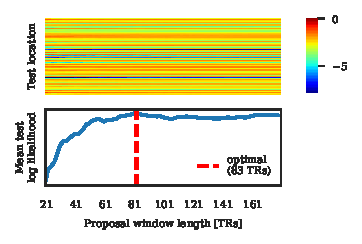
\includegraphics[width=0.47\textwidth]{fig/studies/cross_validating_sliding_windows/sw_cv_results_df_null}
  }
  \subcaptionbox{Fast-changing structure\label{fig:sw-cv-demo-fast-changing-structure}}{
    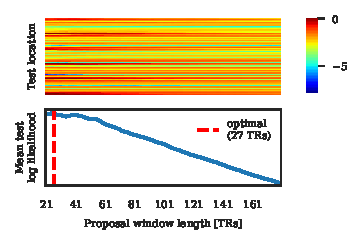
\includegraphics[width=0.47\textwidth]{fig/studies/cross_validating_sliding_windows/sw_cv_results_df_periodic_3}
  }
  \caption{
    Cross-validated sliding-windows demonstration showing how the optimal window length adapts to the underlying covariance structure.
    Heatmap colormaps indicate test location log likelihoods.
    Line plots show the mean test log likelihood over all test locations.
  }\label{fig:sw-cv-demo}
\end{figure}


\info[inline]{Paragraph: Discuss our particular implementation.}
The minimum and maximum window exploration lengths are set based on theoretical insights gathered over the past decade.
We leverage the existing wisdom in the field to choose $w_{min}$ and $w_{max}$ as 20~\parencite{Leonardi2015} and 180 seconds.
These are rounded up to the nearest odd number of \glspl{tr} to ensure symmetry.
%
The minimum window length ensures that we do not filter out signal in (expected) relevant frequency bands.
There is no actual constraint on maximum proposal window length limit.
If the signal is fundamentally static, we would expect the window length to trend to infinity.
However, doing so reduces the number of available evaluation points, so we are left with a trade-off.
%
After the optimal window length is determined, \gls{tvfc} estimates are generated in the same way as the regular \gls{sw} approach as discussed in \cref{subsec:sliding-windows-fc}.
%
Empirically, we show that this window length does indeed match the expected window length behavior on simulated data (see \cref{sec:simulations-results}).

\clearpage
\section{The Wishart process}
\label{sec:wishart-process}
%%%%%

\info[inline]{Paragraph: Introduce Wishart process and its history and application.}
In this section we introduce the \gls{wp} to the task of estimating \gls{tvfc}.
Described by \textcite{Bru1991} as matrix generalizations of square Bessel processes, the \gls{wp} is a stochastic matrix process consisting of (for our intents and purposes) covariance matrices.
\textcite{Wilson2010} described a more modern and generalized version of this stochastic process.
%
We discuss its basic construction as well as any required adaptation and fine-tuning to the field of neuroimaging.
We note that many additional improvements and tweaks are still possible, and promising future work directions are discussed in \cref{subsec:model-extensions}.
Model parameters are inferred through \gls{vi}, an approximate inference routine.
The promise of \glspl{wp} is presented by \textcite{Wilson2010, Heaukulani2019} as well, where it is shown that it outperforms \gls{mgarch} models on a range of data sets.

As we enter the domain of Bayesian machine learning~\parencite{Ghahramani2015}, familiarity with concepts from excellent textbooks such as \textcite{MacKay2002, Bishop2006, Hastie2009, Murphy2012, Murphy2023} will prove helpful.

%%
\subsection{The Wishart distribution}
\label{subsec:wishart-distribution}
%%

\info[inline]{Paragraph: Introduce Wishart distribution.}
The Wishart \emph{distribution} defines a probability density function over $D \times D$ symmetric positive definite matrices $\mathbf{\Sigma}$:
\begin{equation}
  f(\mathbf{\Sigma}|\mathbf{V},\nu) = \frac{1}{Z} |\mathbf{\Sigma}|^{(\nu - D - 1)/2} \exp{(-\frac12tr(\mathbf{V}^{-1}\mathbf{\Sigma}))},
\end{equation}
where $\mathbf{V}$ is a $D \times D$ positive definite scale matrix, and $\nu \geq D$ is the number of degrees of freedom.
The normalization constant $Z$ is given by $2^{\nu D/2}|\mathbf{V}|^{\nu/2}\Gamma_D(\nu/2)$, where $\Gamma_D(\cdot)$ is the multivariate gamma function:
\begin{equation}
  \Gamma_D(\nu/2) = \pi^{D(D-1)/4} \prod_{j=1}^D \Gamma(\nu/2 + (1-j)/2).
\end{equation}
This distribution has mean $\nu \mathbf{V}$ and mode $(D - \nu - 1)\mathbf{V}$ for $\nu \geq D + 1$.

\info[inline]{Paragraph: Discuss Wishart distributed matrix construction.}
Crucially, we can construct a Wishart-distributed random (matrix-valued) variable from a collection of i.i.d.~zero-mean Gaussian random variables.
Namely, the sum of outer products of multivariate Gaussian random variables is Wishart distributed:
\begin{equation}
  \mathbf{\Sigma} = \sum_{i=1}^\nu \textbf{u}_i \textbf{u}_i^T \sim \mathcal{W}_D(\mathbf{V}, \nu),
  \label{eq:wishart-from-iid-gaussians}
\end{equation}
where $\textbf{u}_i$ are i.i.d. $\mathcal{N}(\textbf{0}, \mathbf{V})$ distributed, $D$-dimensional random variables.
$\mathcal{W}_D(\mathbf{V}, \nu)$ denotes a Wishart distribution with $D \times D$ scale matrix $\mathbf{V}$, and $\nu$ degrees of freedom.
We use this property to construct the \gls{wp}.
A matrix constructed in this manner will always be a valid covariance matrix: symmetric and positive semi-definite.

%%
\subsection{Wishart process model definition}
%%

\info[inline]{Paragraph: Define Wishart process model construction.}
For the \gls{wp} definition, we follow notations from~\textcite{Heaukulani2019}.
Let $Y$ := ($\mathbf{y}_n$, $1 \leq n \leq N$) denote a sequence of measurements in $\mathbb{R}^D$.
That is, $\mathbf{y}_n = [y_{n,1}, \dots, y_{n,D}]$.
In \gls{fmri} analyses, $N$ refers to the number of time steps or scan \emph{volumes}, and $D$ refers to the number of node time series (e.g.~number of brain regions for which a characteristic \gls{bold} signal time series is determined).

We denote \textbf{input locations} as $X$ := ($x_n$, $1 \leq n \leq N$) in $\mathbb{R}$.
For \gls{fmri} analyses, the (univariate, 1-dimensional)~$x_n$ here is the time at which measurement $\mathbf{y}_n$ is taken (observed).\footnote{Our model construction does not \emph{require} the input locations to be univariate. One could, for example, add other (side) information of interest such as the decaying magnet strength during a scan, head motion~\parencite[often considered one of the most significant confounding factors, see e.g.][]{Laumann2017}, a design matrix for \gls{tb-fmri}, arousal (e.g. as measured by pupil diameter or eyelid closure), and/or physiological signals such as heart rate. Whether this is beneficial will require further validation studies.}
In our model definition the spacing between values of $x_n$ may be irregular and does not need to be constant.
Even though we expect \gls{fmri} data to be organized in a grid-like fashion of regular time intervals of a single \gls{tr}, this model flexibility could still be useful.
For example, it allows for naturally leaving out a measurement due to an artifact.
From the Bayesian perspective, we just so happen to make \emph{observations} at fixed intervals (giving the impression of a state-space structure), but this may not reflect the underlying process.
For computational ease-of-use we consider $X$ (the scan frame times) in the fixed interval of [0, 1] during training and prediction.
Estimates are then scaled back to the scan time frame.

We let the conditional likelihood of observations be multivariate Gaussian:
\begin{equation}
  \mathbf{y}_n \mid \boldsymbol{\mu}_n, \mathbf{\Sigma}_n \sim \mathcal{N}(\boldsymbol{\mu}_n, \mathbf{\Sigma}_n),
\end{equation}
where $\mathbf{\Sigma}_n$ is a $D \times D$ covariance matrix.
This is a researcher choice; other likelihood functions such as the multivariate $t$-distribution could be implemented instead.
In dealing with \gls{fmri} data, we may assume all entries of the mean vector~$\boldsymbol{\mu}_n$ to be zero, so this likelihood simplifies to
\begin{equation}
  \mathbf{y}_n \mid \mathbf{\Sigma}_n \sim \mathcal{N}(\textbf{0}, \mathbf{\Sigma}_n).
\end{equation}
In our context, we are not interested in the actual values of $\mathbf{y}_n$.
Instead, we are interested in the (random) process $\mathbf{\Sigma}_1, \mathbf{\Sigma}_2, \dots, \mathbf{\Sigma}_N$.
This process constitutes the \gls{tvfc} as described in \cref{sec:tvfc}.
Again, this covariance process (or \emph{structure}) is never directly observed.

As mentioned before, a Wishart distributed random (matrix-valued) variable can be constructed from i.i.d.\ collections of Gaussian random variables.
Analogously, we can construct \glspl{wp} from i.i.d.~collections of Gaussian \emph{processes}~\parencite{Rasmussen2006}.\footnote{\textcite{Gourieroux2009} construct \glspl{wp} is a similar fashion, but instead of \glspl{gp} they use (stochastic) vector autoregressive processes as underlying latent processes.}
Let
\begin{equation}
  f_{d,k} \sim GP(\textbf{0}, \mathcal{K}(\cdot, \cdot ; \theta)),
\end{equation}
for $1 \leq d \leq D$ and $1 \leq k \leq \nu$, where $\mathcal{K}(\cdot, \cdot ; \theta)$ refers to a \emph{kernel} function (a.k.a.~covariance function) with respective kernel parameters $\theta$.
It is our job as modelers to choose a suitable kernel function.

Evaluating a \gls{gp} at a given point in time returns a Gaussian distributed random variable.
Let $F_{n,d,k} := f_{d,k}(X_n)$ denote the evaluation of the \gls{gp} at point $X_n$.
Under the posterior this is \emph{not} a zero-mean Gaussian variable anymore.
Moreover, unlike with a \gls{gp}, the posterior of the \gls{wp} is \emph{not} a \gls{wp}.

We write $\mathbf{F}_n$ for the aggregate (random) $D \times \nu$ matrix $(F_{n,d,k})_{1\leq d\leq D,1\leq k\leq \nu}$, which has entries $F_{n,d,k}$, indexed by $d$ and $k$.
Analogues to \cref{eq:wishart-from-iid-gaussians}, we can then construct
\begin{equation}
\label{eq:sigma-definition}
  \mathbf{\Sigma}_n = \mathbf{A} \mathbf{F}_n \mathbf{F}_n^T \mathbf{A}^T
\end{equation}
as a Wishart-distributed random matrix at time $n$.

This construction allows us to query at any point in time, as the underlying \glspl{gp} can be queried at any value of $x_n$.
We make sure $\mathbf{A} \in \mathbb{R}^{D \times D}$ is restricted so that \emph{scale matrix} $\mathbf{A}\mathbf{A}^T$ is positive definite.
Recall that $\mathbf{A}\mathbf{A}^T$ corresponds to the scale matrix $\mathbf{V}$ as discussed in \cref{subsec:wishart-distribution}.
That is, $\mathbf{A}$ is the Cholesky factor of $\mathbf{V}$.
The scale matrix covariance terms can be considered mean covariances across the time series.
We train matrix $\mathbf{A}$ as part of the inference routine.
Intuitively, for a static covariance estimate, our \gls{wp} could simply learn these $\mathbf{A}$ covariance terms and `switch off' the \glspl{gp}.

Writing it out, our zero mean, multivariate Gaussian likelihood is given by
\begin{equation}
  p(\mathbf{y}_n|\mathbf{\Sigma}_n) = \frac{1}{(2\pi)^{\frac{D}{2}} |\mathbf{\Sigma}_n|^{\frac{1}{2}}} e^{-\frac{1}{2} \mathbf{y}_n \mathbf{\Sigma}_n^{-1} \mathbf{y}_n}.
\end{equation}
Plugging in our construction of $\mathbf{\Sigma}_n$ from \cref{eq:sigma-definition}, we obtain
\begin{equation}
  p(\mathbf{y}_n|\mathbf{A},\mathbf{F}_n) = \frac{1}{(2\pi)^{\frac{D}{2}} |\mathbf{A} \mathbf{F}_n \mathbf{F}_n^T \mathbf{A}^T|^{\frac{1}{2}}} e^{-\frac{1}{2} \mathbf{y}_n (\mathbf{A} \mathbf{F}_n \mathbf{F}_n^T \mathbf{A}^T)^{-1} \mathbf{y}_n}.
\end{equation}
The log of this likelihood is given by
\begin{equation}
  \log p(\mathbf{y}_n|\mathbf{A},\mathbf{F}_n) = - \frac{D}{2} \log 2\pi - \frac{1}{2} \log |\mathbf{A} \mathbf{F}_n \mathbf{F}_n^T \mathbf{A}^T| - \frac{1}{2} \mathbf{y}_n^T (\mathbf{A} \mathbf{F}_n \mathbf{F}_n^T \mathbf{A}^T)^{-1} \mathbf{y}_n.
\end{equation}

In Bayesian model definition, apart from a likelihood, we have to choose a prior.
We choose a fully factorized prior over $F$.
This is typically considered a fair assumption, as independence in the prior does not lead to independence in the posterior.
That is,
\begin{equation}
  p(F) = \prod_{n=1}^N p(\mathbf{F}_n) = \prod_{n=1}^N \left[ \prod_{d=1}^D \prod_{k=1}^\nu f_{d,k}(X_n) \right].
\end{equation}

We know that $Y_n$ only depends on $\mathbf{F}_n$, so $p(Y|F) = \prod_{n=1}^N p(\mathbf{y}_n|\mathbf{A},\mathbf{F}_n)$.
Since all entries of $\mathbf{F}_n$ are~i.i.d., we can write
\begin{equation}
  p(Y,F) = p(Y|F)p(F) = \prod_{n=1}^N \left[ p(\mathbf{y}_n|\mathbf{A},\mathbf{F}_n)) \prod_{d=1}^D \prod_{k=1}^\nu f_{d,k}(X_n) \right].
\end{equation}

Recall that we want correlation in $Y$.
With independence in $\mathbf{F}_n$, we do get such correlation in $\mathbf{\Sigma}$.

%%
\subsection{Variational Wishart processes}
%%

\info[inline]{Paragraph: Describe (variational) inference routine.}
We are interested in the posterior
\begin{equation}
  p(F|Y) = \frac{p(Y,F)}{p(Y)},
\end{equation}
where computing $p(Y) = \int p(Y|F)p(F)dF$, the marginal density of observations or \emph{evidence}, is intractable.
We therefore resort to \textbf{approximate inference} routines.

\Gls{vi} is a technique that approximates a probability density through \emph{optimization}~\parencite{Jordan1999, Hoffman2015, Blei2017}.
It is usually faster and more scalable than other inference methods, such as \gls{mcmc} sampling~\parencite[as used in e.g.][]{Fox2011}, especially with larger data sets.
In fact, the recent advances that made this style of inference possible explains the `why now' of introducing this model to the task of \gls{tvfc} estimation.

With \gls{vi}, we posit a family of distributions~$q(F)$ over the latent variables and then find the member of that family which is close to the target distribution (the true posterior)~$p(F|Y)$.
Closeness here is measured by \gls{kl-divergence}.
The key is to define this family~$q(F)$ to be flexible enough to capture a density close to the posterior, but simple enough for efficient optimization.

We collectively denote $F_{d,k} := (F_{n,d,k}, n \leq N)$.
We choose the variational approximation to the posterior distribution of the latent variables to take the following form:
\begin{equation}
  q(F_{d,k}) \sim \mathcal{N}(F_{d,k};\boldsymbol{\mu}_{d,k}, \mathbf{S}_{d,k}),
\end{equation}
for some \textbf{variational parameters} $\boldsymbol{\mu}_{d,k} \in \mathbb{R}^N$ and $\mathbf{S}_{d,k} \in \mathbb{R}^{N \times N}$ a real, symmetric, positive definite matrix.
We train these parameters together with $\mathbf{A}$ and kernel parameters $\theta$.

Recall that \gls{kl-divergence} is defined as
\begin{equation}
  \operatorname{KL}(q(F)~\|~p(F | Y)) = \mathbb{E}_{q(F)}[\log q(F)] - \mathbb{E}_{q(F)}[\log p(F | Y)].
\end{equation}
Expanding the conditional, we can write
\begin{equation}
  \operatorname{KL}(q(F)~\|~p(F | Y)) = \mathbb{E}_{q(F)}[\log q(F)] - \mathbb{E}_{q(F)}[\log p(F, Y)] + \log p(Y)
\end{equation}
In \gls{vi} we optimize the \gls{elbo}, which is equivalent to this \gls{kl} term up to an added constant:
\begin{equation} \label{eq1}
  \begin{split}
    ELBO & = \mathbb{E}_{q(F)}[\log p(F, Y)] - \mathbb{E}_{q(F)}[\log q(F)] \\
    & = \mathbb{E}_{q(F)}[\log p(Y|F)] - \operatorname{KL}(q(F)~\|~p(F)).
  \end{split}
\end{equation}

The first term of the \gls{elbo} is a likelihood (model fit) term and the second term encourages densities close to the prior (i.e.~it can be considered a complexity penalty).

We make a \emph{mean-field} (fully factorized) simplification for $q(F)$:
\begin{equation}
  q(F) = \prod_{d=1}^D \prod_{k=1}^\nu q(F_{d,k}).
\end{equation}
Our \gls{elbo} is then given by
\begin{equation}
  ELBO = \sum^N_{n=1} \mathbb{E}_{q(\mathbf{F}_n)} [\log p(Y_n|\mathbf{F}_n)] - \sum^D_{d=1} \sum^\nu_{k=1} \operatorname{KL}(q(F_{d,k})~\|~p(F_{d,k})).
\end{equation}

We iteratively maximize this as our objective function, using gradient descent.
In order to be able to compute (approximate) gradients we use the `reparametrization trick' as discussed in \textcite{Salimans2013, Kingma2014}.
This boils down to taking samples (Monte Carlo estimates) of our objective function and computing gradients based on these.

%%
\subsection{Additive white noise model}
%%

\info[inline]{Paragraph: Discuss why and how we need to add white noise.}
Following \textcite{Heaukulani2019}, we introduce additive white noise to make inference more robust.
We empirically validated that this is a necessary step to ensure robust inference.
A small amount of noise is added to $f_n$, to avoid values blowing up when $f_n$ is close to zero when taking the inverse.
This means we redefine and update the covariance matrix of $\mathbf{y}_n$ from \cref{eq:sigma-definition} slightly as
\begin{equation}
  \mathbf{\Sigma}_n = \mathbf{A} \mathbf{F}_n \mathbf{F}_n^T \mathbf{A}^T + \mathbf{\Lambda},
\end{equation}
where $\mathbf{\Lambda}$ is the additive noise matrix; a diagonal $D \times D$ matrix with positive (diagonal) entries.
Diagonal values are initialized as 0.01 and are trained with the rest of the before-mentioned model parameters (off-diagonal values remain zero).
This modification may be interpreted as introducing white (or \emph{observational}) noise to the model.

%%
\subsection{Sparse variational Wishart processes}
\label{subsec:svwp}
%%

The beauty of basing our \gls{wp} construction on underlying \glspl{gp}, is that we can take advantage of the rapid development and improvement of these models~\parencite[echoing sentiments from][]{Foti2019}.

\glspl{gp} are known to not scale well with large data sets~\parencite{Rasmussen2006}.
When $N$ is large,\footnote{The official \texttt{GPflow} documentation defines `large' as $N > 1000$.} a popular approach to make such models more computationally viable is to use \emph{sparse} variational \glspl{gp}~\parencite{Titsias2009, Hensman2013, Matthews2016}.
These introduce the concept of \emph{inducing points}~\parencite{Bauer2016}.
Such points can be considered learned, auxiliary data points (a.k.a.~pseudo-inputs).
The number of inducing points ($M$) is typically much smaller than $N$.
After training, the model only uses said points to infer and make predictions, rendering a trained model \emph{independent} from the training data.
This approach thus assumes that there is redundant information in the data set.

In \gls{fmri} scans, the size of $N$ tends not to be problematic, as the time needed to take a full measurement of the brain or a subset thereof (the sampling period or \gls{tr}) is typically in the order of 0.5 to 2 seconds.
However, when applying this model to other neuroimaging modalities with higher temporal resolution (such as \gls{eeg}) a sparse implementation is the only viable option.
For example, from \cref{fig:wp-computational-cost} we observe that training times scale dramatically with increased $N$ and $D$.
We will return to this in \cref{subsec:model-extensions}.

Our \gls{svwp} model is identical to the \gls{vwp}, except that its underlying \glspl{gp} are sparse.


\begin{figure}[t]
  \centering
  \subcaptionbox{VWP \label{fig:vwp-computational-complexity}}{
    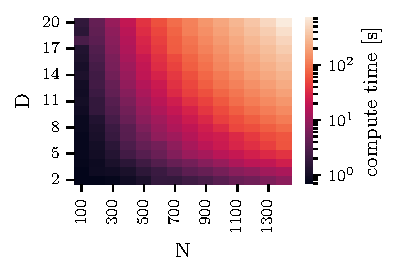
\includegraphics[width=0.47\textwidth]{fig/studies/wp_computational_cost/VWP}
  }
  \subcaptionbox{SVWP \label{fig:svwp-computational-complexity}}{
    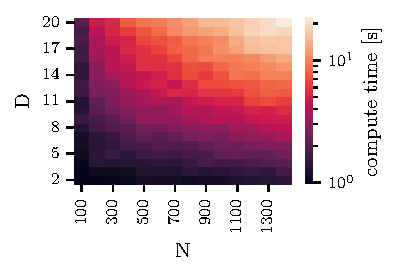
\includegraphics[width=0.47\textwidth]{fig/studies/wp_computational_cost/SVWP}
  }
  \caption{
    WP computational complexity as a function of $N$ and $D$.
    Shown is time required (in seconds) to complete 4 epochs.
    Run on a 3 GHz Intel Core i5 CPU.
  }
  \label{fig:wp-computational-cost}
\end{figure}


%%
\subsection{Implementation details}
%%

\info[inline]{Paragraph: Discuss implementational details.}
Throughout all benchmarks and experiments in this thesis, we use a (stationary, isotropic) Matérn 5/2 kernel, given by
\begin{equation}
  \label{eq:matern}
  k(\textbf{x}, \textbf{x}') = \sigma^2 (1 + \sqrt{5} r + \frac53 r^2) \exp(-\sqrt{5}r),
\end{equation}
with $r = \frac{||\textbf{x} - \textbf{x}'||}{l}$, and where $l$ and $\sigma$ are the kernel length scales and variance parameters, respectively, which are trained.
Their initial values are set to~0.3 and~1.0, respectively.
These parameters are part of the total set of model parameters~$\theta$.
This kernel is a twice differentiable covariance.
The popular radial basis function (RBF), also known as squared exponential or Gaussian, kernel is considered too smooth for our purposes (this kernel is infinitely differentiable), see \cref{fig:kernel-draws} as well.
We note that kernel choice imposes assumptions (i.e.~inductive bias) on the behavior of observed time series~\parencite[see also][chapter 2]{Duvenaud2014}.
For example, all Matérn kernels assume data stationarity.
Kernel functions can be considered as a specification of similarity between observations.
Our kernel considers further away observations less similar.
But a periodic kernel, for example, could consider a further away points \emph{more} similar if it is in phase with another point.
Or, as with the Gibbs kernel, kernel parameters could themselves be a function of input features $\mathbf{x}$ (e.g.~time).
In fact, this is one of the exciting aspects of the \gls{wp}.
We can characterize time series through these kernels.
Smoothness of correlation structure can be expressed by such kernel functions for example~\parencite{Fyshe2012, Fox2015, Foti2019}.
Kernels can be combined too; sums and products of kernels are also valid kernels.
As such more expressive kernels can be designed~\parencite{Gonen2011}.
Kernel choice requires trial-and-error, although some efforts have been made to automate this process~\parencite[see e.g.][]{Steinruecken2019}.


\begin{figure}[t]
  \centering
  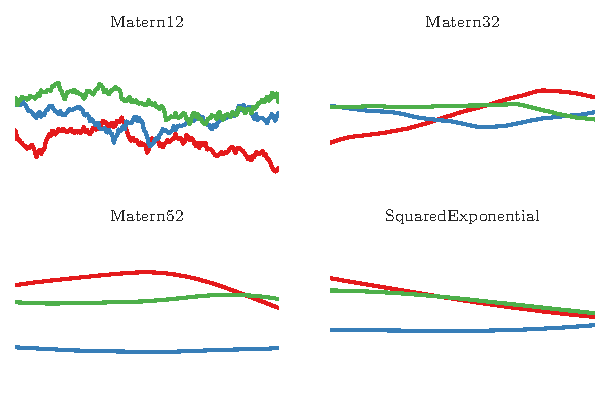
\includegraphics[width=\textwidth]{fig/studies/kernels}
  \caption{
    Draws from common Gaussian process kernels on interval $\left[ {0,1} \right]$.
  }
  \label{fig:kernel-draws}
\end{figure}


For all benchmarks and experiments we set $\nu = D$.
Larger values of $\nu$ have been tried empirically without improvement.
In general, it is best to keep $\nu$ small, as computational cost also scales with $\nu$.

We run both the \gls{vwp} and \gls{svwp} models in most experiments, although only the former for cases with $N \leq 200$ and only the latter for cases with $N \geq 400$.
The number of inducing points is set to $M = 200$, irrespective of time series lengths~$N$.

Standing on the shoulders of giants, the model is implemented using the open-source Python library \texttt{GPflow}~\parencite[][version 2.5.2]{Matthews2017, Wilk2020}.
This \gls{gp} toolbox in turn is built on top of Google's \texttt{Tensorflow}~\parencite[][version 2.9.2]{Tensorflow2015}.
These packages take care of all underlying automatic differentiation.
This means that the amount of code to write is minimal and consists mainly of implementing a (customized) likelihood function.
For these reasons, this black-box implementation~\parencite{Ranganath2014} is simple and fast compared to proposed inference routines based on \gls{mcmc}.
%
In fact, this is crucial insight.
While we acknowledge the \gls{wp} as a complex model, and thus incur its accompanying cost, in return we get a favorable optimization routine that is robust and relatively straightforward.
Contrast this with the \gls{sw} approach, which is trivial in its description, but not straightforward in its implementation, with researchers facing many (arbitrary) implementational decisions to make.
Parameters are updated through gradient descent with Adam~\parencite{Kingma2015} with an initial learning rate of $\alpha = 0.001$.
All \gls{wp} \gls{tvfc} estimation figures in this thesis include the confidence interval of mean estimate plus/minus two standard deviations (i.e.~95\% of the mass of the \gls{wp}), based on 3,000 samples from the posterior.

\clearpage
\section{Extracting TVFC-based features and biomarkers}\label{sec:tvfc-feature-extraction}
%%%%%

\info[inline]{Paragraph: Introduce importance of feature extraction.}
For a given scan, \gls{tvfc} is estimated as a rather large $N \times D \times D$ tensor.
This contrasts \gls{sfc} analyses, where the $N \times D$ data is typically \emph{reduced} in dimensionality to~$D \times D$.
%
In most practical settings and applications, however, we wish to study more interpretable features.
Therefore, it is important to extract features (or \emph{biomarkers} in neuroscientific and clinical contexts) from our predicted correlation structure.
Here we discuss several of such features that will be used in the ensuing chapters.
Details on how exactly they are computed and their relevance for cognition and depression will be discussed in the respective chapters.

\info[inline]{Paragraph: Discuss what we want from extracted features.}
Any data processing step cannot add any information, but merely destroy it.
Therefore, feature extraction should encompass information preservation while removing redundant information (for the task at hand) and noise.
If we desire to use our estimated \gls{tvfc} in some practical application to make predictions, perhaps this estimation can be skipped.
Models can then be trained directly on node time series data.
However, in our context we are interested in the covariance structure itself; as a wiring diagram of the functional interactions within the brain.
%
Extracting features is a crucial step when planning to run any supervised learning algorithm.
In fact, it has been argued that the strong performance of artificial neural networks may be due to their ability to automatically extract meaningful features from data (in contrast to features hand-crafted by humans).

%%
\subsection{TVFC summary measures}\label{subsec:tvfc-summary-measures}
%%

One common way to extract features in \gls{tvfc} neuroimaging is to take edgewise summary measures (or \emph{statistics}) across time.
%
Typical summary measures include the mean~\parencite[analogous to \gls{sfc} estimates; sometimes considered the connection `strength', see e.g.][]{Choe2017} and standard deviation or variance~\parencite[see e.g.][]{Chang2010, Hutchison2013b, Kucyi2013, Kucyi2014, Kaiser2015, Demirtas2016, Choe2017}.
Variance (or standard deviation) is sometimes interpreted to represent connectivity `stability' or `flexibility'~\parencite[see e.g.][]{Allen2014}.
However, we need to be vigilant with vague terminology and premature interpretations.

More precisely, \gls{tvfc} means are calculated as
\begin{equation}
  \mu_{i,j} = \frac{1}{N} \sum_{n=1}^N \mathbf{\Sigma}_{n,i,j},
\end{equation}
and \gls{tvfc} variances are calculated as
\begin{equation}
  \sigma^2_{i,j} = \frac{1}{N} \sum_{n=1}^N (\mathbf{\Sigma}_{n,i,j} - \mu_{i,j})^2,
\end{equation}
for the edge between nodes $1 \leq i \leq D$ and $1 \leq j \leq D$.

Here we propose an additional summary measure, the \gls{tvfc} \textbf{rate-of-change}, defined as the mean absolute relative difference per subsequent time steps:
\begin{equation}
  r_{i,j} = \frac{1}{N-1} \sum_{n=2}^N | \frac{\mathbf{\Sigma}_{n,i,j}}{\mathbf{\Sigma}_{n-1,i,j}} - 1 |,
\end{equation}
for the edge between nodes $1 \leq i \leq D$ and $1 \leq j \leq D$.
This summary measure captures how smooth a time series is over time (i.e.~the smoothness of the estimated \gls{fc} time series in our case).
It is more informative of \gls{fc} frequency amplitudes and is akin to \gls{fc} `variability' as described in \textcite{Allen2014}.
To illustrate its relevance, this summary measure can distinguish two sine waves with identical mean and variance, yet oscillating at different frequencies (see e.g. \cref{fig:synthetic-covariance-structures}).
As such it is complementary to the other two summary measures.

%%
\subsection{Brain states and related metrics}\label{subsec:brain-states}
%%

Another common way to reduce the dimensionality of \gls{tvfc} estimates is to assume that the estimated covariance structure at each time point can be characterized as a certain `brain state' (or `\gls{fc} state')~\parencite{Kringelbach2020}.
Such states are short-term, recurring spatial activity \gls{fc} patterns across time and subjects.
In our context, they are characterized by an \gls{fc} correlation matrix.
%
The existence of such a state-space structure in the brain has been shown to be a valid view~\parencite{Deco2015}.
%
These states can be insightful on their own or can be used as extracted features.
For example, \textcite{Rashid2016} showed that schizophrenia patients spend more time in low-contrast states.
One exciting aspect of the construct of brain states is that they can be synthesized across species and imaging modalities (e.g.~with microstates in \gls{eeg}, see \textcite{Allen2014} for further discussion).
As such they can serve as a common language to bridge multiple levels of neuroscientific research.

Brain states are typically extracted either by using $k$-means clustering on estimated \gls{tvfc}~\parencite[see e.g.][]{Allen2014, Abrol2016, Zhi2018, Hakimdavoodi2020} or using models (usually \glspl{hmm}, see \cref{subsec:state-based-models}) that have this states assumption baked into their definition~\parencite{Lurie2020}.
In such latter cases we do not estimate the full \gls{tvfc} tensor.
Thus, certain information is lost in the process.

Here we extract brain states from estimated \gls{tvfc} using the original $k$-means algorithm described in \textcite{Lloyd1982}.
All estimated correlation matrices for all~$N$ time steps and all subjects are concatenated and fed into this algorithm.
The $k$-means algorithm requires a pre-specified number of clusters~$k$.
One common trick to determine this number is to plot an `elbow curve'~\parencite[see e.g.][chapter 5.5]{Everitt2011}.
Such a plot computes the summed distance between each correlation matrix and its closest (i.e.~assigned) basis state for a range of values of~$k$.
The optimal value of~$k$ is then chosen as the one where this curve has an `elbow'; that is, after which the curve is relatively linear and after which adding another cluster does not result in a big decrease thereof.
%
Perhaps surprisingly, most studies using brain states to summarize the brain's activity find a relatively small number of distinct states, for example three in \textcite{Choe2017, Dini2021} and 12 in \textcite{Vidaurre2017}.

Even though the \gls{wp} is not constrained in estimating \gls{tvfc} in grid-like fashion, we do this for extracting brain states to allow for better comparison to other methods.
However, we could estimate as many covariance matrices at as high of a temporal resolution as we like for this task.
%
Furthermore, some studies have relaxed the assumption that participants are assigned to a single state and learn a weight vector over all basis states instead for each time step~\parencite{Leonardi2014}.
Such an approach again blurs the boundary between the continuous modeling of brain activity and viewing the brain as a state-space system.
The latter view is still debated~\parencite[see][for an excellent discussion on the potential and shortcomings of the brain states framework]{Keilholz2017}.

%%
\subsubsection{Brain state metrics}
%%

If our estimation method produces brain states, we can also extract interpretable features from these.
These include global metrics such as brain state switching rate (how frequently participants switch between states),
and state-specific metrics such as occupancy rate and dwell time (the relative time participants spend in each state).

%%
\subsection{Graph theoretic analysis}\label{subsec:graph-theoretic-analysis}
%%

Yet another common feature set extracted from \gls{tvfc} is to (mathematically) represent brain network connectivity as a graph and then compute graph theoretic metrics~\parencite{Sporns2011}.
Such approaches can be used to study topological properties of brain networks and the properties of connectivity in the brain.
In graph theory, brain \glspl{roi} are represented as \textbf{nodes}.
The \textbf{edges} between brain regions can take many forms.
As mentioned before, throughout this thesis we will use the terminology of nodes and edges to describe brain regions and their respective connections.

It is common to use \gls{rs-fmri} and define edge strength as a given \gls{fc} metric (often, and in our case as well, correlation).
Edges can be thresholded and binarized, but weighted graphs are also common.
Standard graph approaches are typically used on graphs defined by \gls{sfc}, such as decomposing networks into modules~\parencite{Betzel2016}, detecting hubs, and computing graph metrics.
Such graph metrics fall into one of three categories: global properties (e.g.~global efficiency and path length), modularity, and local properties (e.g.~clustering).

Neuroscientists have increasingly adopted techniques from the field of network science.
Graph theoretic concepts such as centrality, efficiency, network modularity~\parencite{Zalesky2014}, and community structure have been extracted from brain networks.
For dynamic networks, such changes have been related to learning~\parencite{Bassett2011}.
Such dynamic changes have had a significant impact on basic neuroscience in understanding concepts such as the dynamics of integration and segregation in the brain, including in understanding disorders such as depression~\parencite{Gong2015}.

Some controversy remains in graph theoretic studies.
First, some graph metrics may not be applicable to the data at hand.
Graph \emph{efficiency}, for example, assumes causal connections between nodes, and may not be valid in (undirected) graphs defined by \gls{fc}~\parencite{Chen2017}.
Secondly, the interpretation of graph metrics often leaves much to speculation.

%%
\subsubsection{Dynamic graph theoretic metrics}
%%

As this thesis is concerned with dynamics of brain activity, we would want to study time-varying properties of graphs and graph theoretic metrics.
However, this field has not received much attention yet.
%
In the simplest case these could be summary measures of graph metrics across time again.
\textcite{Zalesky2014} demonstrated the synthesis of \gls{tvfc} with graph theory.
Some dynamic graph studies have been run~\parencite{Bassett2011, Bassett2013}.
This is a newer approach, but we may take inspiration from the field of temporal network theory~\parencite{Holme2012, Yu2015, Thompson2017}.

%%
\subsection{Feature extraction from models}\label{subsec:model-features}
%%

Instead of merely describing or estimating covariance, such as the \gls{sw} approach, the \gls{wp} is a generative model.
Like \gls{dcc}, it is a model-based approach.
Thus, we have a full model for each scan and subject.
Assuming we have a good model of the underlying process, we may be able to extract relevant process or subject features.

An example would be the learned \gls{wp} kernel lengthscale $l$, see \cref{eq:matern}, which could be extracted from the trained models and compared between subjects and scan times.
The reverse may also be interesting.
For example, in a similar Bayesian model approach, \textcite{Li2019a} defined the prior for their \gls{gp} lengthscale based on their expectation to find frequency dynamics close to the theta range (4--12 Hz).
%
With this in mind, we can make model choices that explicitly return interpretable and cognition-relevant features.
However, \glspl{gp} (and related models) are not considered to be good at feature extraction, since we encode a lot of the data structure into the kernel choice.
This leaves only several hyperparameters that dictate the data description.
Instead, deep learning models might be better feature extractors~\parencite[and have proven useful in other neuroscientific fields, see e.g.][]{Richards2019}, although these typically require a lot of data.
Overall, we consider model-based approaches a promising direction for feature extraction, but one that requires much work still.

\clearpage
\section{The benchmarking framework}\label{sec:benchmark-framework}
%%%%%

\info[inline]{Paragraph: Introduce main concept of benchmarking.}
How do we compare methods and decide which one to use?
We propose to take inspiration from the field of machine learning, which has extensive experience with such problems.
%
When a single optimization target or `learning task' is missing, it is common practice to define a suite of \emph{benchmarks}.
Each benchmark frames method selection as a prediction task and competition~\parencite{Breiman2001, Shmueli2010, Bzdok2018, Khosla2019, Poldrack2020, Tejavibulya2022}.
Such benchmarks need to be uniquely domain specific.
A collection of benchmarks then paints a rich picture of which methods are more sensitive or specific, what the failure modes of each method are, and ultimately leads to practical guidelines on which method should be used in each real-life situation.\footnote{In many machine learning sub-fields benchmarks are framed as clearly defined targets, such as as image classification accuracy. A more apt comparison may be \gls{nlp}, where optimization targets are not straightforward, and a \emph{range} of desired targets are evaluated per model~\parencite[see e.g.][]{Bommasani2021}.}
This is a live process, and insights and approaches are updated as time goes by.
%
In fact, this shift in focus toward \emph{predictive} methods is increasingly argued for in neuroscience, especially for translational work to clinic practice~\parencite{Yarkoni2017, Leenings2022, Voytek2022}.
While the focus on benchmarks is relatively new in neuroimaging and psychology, it has existed in computer science and biomedical contexts for a long time,\footnote{In machine learning research, for example, the first large benchmark (ImageNet) was launched back in 2010~\parencite{Deng2009}. Image classification performance has dramatically increased since.} and we can learn a lot from their experiences~\parencite{Leenings2022}.
%
One such lesson is that benchmarks are not a silver bullet.
There are risks involved with a hyper-focus on benchmarks, such as often discussed in the case of machine learning research~\parencite{Wagstaff2012, Sculley2018}.
This field has also been considered to have its fair share of a reproducibility crisis~\parencite[see also][]{Bell2021}.

In fact, it can be argued that settling on good benchmarks is more important than model development.
Once benchmarks are in place, model development can be automatic and fast.

\info[inline]{Paragraph: Overview of existing benchmarks.}
Many benchmarks have already been proposed (either explicitly or implicitly) in the field.
However, a collectively agreed upon set is still missing and benchmarks remain scattered.
We do note the increase in initiatives to publish open-source data sets, which is a prerequisite for benchmarking as a community~\parencite{Gorgolewski2016, Kennedy2016, Nichols2017, Leenings2022}.
Throughout this thesis we aim to strike a balance between using benchmarks (or variations thereof) that others have looked at, and proposing new ones that contribute to the field.
Despite the heterogeneity of benchmarks, most can be categorized into one of the following buckets.

%%
\subsection{Simulations benchmarks}\label{subsec:simulation-benchmarks}
%%

\info[inline]{Paragraph: Describe general idea behind simulation benchmarks.}
In \textbf{simulation benchmarks}, time series are generated by a process with a known, pre-specified underlying covariance structure~\parencite[see e.g.][]{Sakoglu2010, Lindquist2014, Hindriks2016, Shakil2016, Lan2017, Monti2017, Taghia2017, Thompson2018, Warnick2018, Li2019b, Ebrahimi2020}.
Such a specified covariance structure can be deterministic or random.
%
The prediction task is then to `reconstruct' this ground truth covariance structure from the simulated observations.
Performance is measured as the difference between estimated \gls{tvfc} and ground truth values.
Methods with lower \emph{reconstruction error} are then considered superior.
%
This benchmark is the most common in literature.
In fact, \textcite{Thompson2018} already proposed a common framework to benchmark \gls{tvfc} methods on simulated data.
%
Furthermore, we use the simulations as motivating examples of why it is important to benchmark estimation methods.

\info[inline]{Paragraph: Describe advantages and disadvantages of this class of benchmarks.}
One attractive characteristic of this family of benchmarks is that it provides flexibility to explore different edge cases and to find failure modes and qualitative characteristics for a given method.
Appropriate methods should both be \emph{sensitive} to covariance structure present in the (noisy) data, as well as \emph{specific} not to return any spurious structure where there is none~\parencite{Leonardi2015}.
%
The major downside is that it is not clear how to define a realistic covariance structure and noise routine.
Therefore, it is not clear how results generalize to the more realistic scenarios in which the methods will be used.

\info[inline]{Paragraph: Discuss more drawbacks and caveats of simulation-based benchmarks.}
Simulation studies in \gls{fmri} are challenging because of the complexity of the underlying generative process~\parencite{Welvaert2014}.
This highlights the need for benchmarks based on ground truth data.
%
Furthermore, simulations may be \emph{too} flexible.
Most studies that proposed new methods for estimating \gls{tvfc} introduced their own simulation paradigm.
Without a suite of synthetic covariance structures and simulation protocols that are considered relevant and agreed upon by the community, methods comparison will continue to face skepticism and controversy.
%
In the earlier benchmarking of \gls{tvfc} estimation methods on simulated data, \textcite{Thompson2018} proposed a set of four simulated data studies that allowed for fair comparison of proposed methods.
The code for this framework was open-sourced and designed in such a way that other researchers could build on it.
The first tests how similar the estimates from the different methods are.
Strongly correlated predictions from methods may indicate that these methods capture similar aspects of the signal.
The second tests for \emph{sensitivity} to changing covariance structure.
The third tests for \emph{robustness} when the mean of the time series changes.
The fourth tests how well the methods can detect sudden changes (see also \cref{subsec:sudden-changes}).
Their simulations are constructed with autocorrelation effects, based on assumed structure in real \gls{fmri} data.
Here we propose to achieve such structure by imposing real data on the simulated data.
While we underwrite the philosophy behind this benchmarking framework, it still has its limitations.
For example, it only considers the bivariate ($D = 2$) case and does not include any actual \gls{fmri} data studies.
Perhaps this has played a role in why the work has had little impact on \gls{tvfc} estimation in practice so far.

%%
\subsection{Resting-state fMRI benchmarks}
%%

\info[inline]{Paragraph: Describe general idea behind rs-fMRI benchmarks.}
In benchmarks based on \gls{rs-fmri} data, it is common to look at the predictive power of estimated \gls{tvfc}.
This could be the behavioral performance on some task, subject measures and phenotypes, or cognitive states.
In the absence of an external stimulus, it is thought that \gls{rs-fmri} can illuminate the brain's functional architecture.
It has been demonstrated that individual differences are embedded in such covariance structures.
In fact, in a so-called `fingerprint' analysis, \textcite{Finn2015} showed that an individual's covariance structure or `connectome' is unique.

\info[inline]{Paragraph: Describe idea behind subject measure prediction benchmarks.}
Typically, the estimated \gls{tvfc} (or features derived from it) are viewed as extracted \emph{biomarkers}.
These are fed to a regressor or classifier to predict either non-clinical~\parencite[see e.g.][]{Taghia2017, Li2019a} or clinical~\parencite[see e.g.][]{Filippi2019, Du2021} subject measures and phenotypes.
Methods that do better at these prediction tasks are then said to have preserved more useful information.
%
In a similar data-driven spirit, \textcite{Li2019a} argued that the controversial data preprocessing step of \gls{gsr} \emph{should} be included since it increases the predictive power of subsequently extracted networks.

\info[inline]{Paragraph: Introduce test-retest robustness studies and frame as benchmark.}
Test-retest robustness studies~\parencite{Noble2019}, although usually not explicitly described as predictive tasks, can be viewed as looking at the predictive power of a first \gls{rs-fmri} scan to predict which subsequent scan belongs to the same subject~\parencite{Fiecas2013, Choe2017, Abrol2017, Zhang2018, Elliott2020}.
These benchmarks are broadly defined and can relate to \gls{sfc}, \gls{tvfc} summary measures~\parencite{Abrol2017, Choe2017}, and brain states~\parencite{Abrol2016} and their related features~\parencite{Abrol2017}.

\info[inline]{Paragraph: Describe advantages and disadvantages of this class of benchmarks.}
One major advantage of using \gls{rs-fmri} over simulations is that it constitutes realistic data.
Most \gls{tvfc} studies have used \gls{rs-fmri} data.
Therefore, results will generalize better to practical use cases.
%
A major advantage of using \gls{rs-fmri} over \gls{tb-fmri} is that the data acquisition and preprocessing pipeline designs can easily be standardized and replicated (and are thus more robust).
Moreover, the data can be used for a variety of purposes, which makes it more attractive for large-scale, multi-site data collection collaborations.
And indeed, such large data sets are readily available for more robust benchmarking~\parencite[see e.g.][]{VanEssen2012, Allen2014b}.
%
A disadvantage of using \gls{rs-fmri} data is that there is no controlled stimulus influencing brain activity.
It is typically not known what subjects were thinking about during the scan~\parencite[see also][]{Finn2021}.

%%
\subsection{Task-based fMRI benchmarks}
%%

\info[inline]{Paragraph: Describe general idea behind tb-fMRI benchmarks.}
In \gls{tb-fmri}~\parencite{Gonzalez-Castillo2018} benchmarks, the goal is often to predict an external event or task~\parencite[see e.g.][]{Sakoglu2010, Glerean2012, Shine2015, Monti2017, Sahib2018, Xie2019} or extract a behaviorally well-known phenomenon~\parencite[see e.g.][]{Lan2017, Warnick2018, Li2019b, Ebrahimi2020}.
Such external stimuli and side information are again considered \emph{proxies} for a ground truth.

\info[inline]{Paragraph: Describe advantages and disadvantages of this class of benchmarks.}
These benchmarks are less common, due to the difficulty of collecting large amounts of standardized data.
Furthermore, test-retest reliability has been found to be especially low in \gls{tb-fmri}~\parencite{Elliott2020}.
A promising idea is to record subjects watching a movie, which combines benefits of \gls{rs-fmri} benchmarks in the sense that it is easy to reproduce and standardize, with those of \gls{tb-fmri} benchmarks because we have some controlled stimuli guidance at known times that influence what subjects are experiencing and processing~\parencite{Eickhoff2020, Finn2021}.
However, movie watching may make the data less multi-purpose and favor visual processing studies.
Furthermore, subjects may pay varying degrees of attention to the stimuli.
Those that pay little attention may exhibit higher activity in visual areas but would otherwise be like participants in \gls{rs-fmri} setups.
We argue that \gls{tb-fmri} are especially powerful for benchmarking specific method characteristics.

%%
\subsection{The imputation benchmark}\label{subsec:imputation-benchmark}
%%

\info[inline]{Paragraph: Describe general idea behind the imputation benchmark.}
This thesis also introduces a new class of benchmarks based on imputation and interpolation.
It uses ground truth data and can be evaluated on any \gls{fmri} data set.
As mentioned before, using a ground truth is important, since in general it is best for a benchmark to be as close to the eventual use case and application as possible.

\info[inline]{Paragraph: Describe imputation benchmark.}
The imputation benchmark works as follows.
A train and test set are defined as data points left out of the original time series.
%
Each method is then tasked to estimate the covariance structure matrices at the test locations, based only on the observations from the train data set.
The performance metric for this benchmark is then the average (test) likelihood to observe the test set time points under a zero-mean Gaussian distribution defined by this estimated covariance structure.
In other words, this benchmark returns the `goodness-of-fit' of model estimates.
%
Train and test splits can be done in many ways.
Each of these tests for something slightly different.
We could leave out a single data point as a test set, a collection of data points, or data points at the end of the time series (which would test forecasting performance).
%
In our experiments, we split up data under a \gls{leoo} scheme (i.e.~an equally sized train and test set split).
%
Determining test location estimates is non-trivial due to the difference in nature of the \gls{tvfc} estimation methods considered.
Since the \gls{wp} is not tied to a certain lattice as its training input or test output, predicting at unobserved data points follows naturally.
For all other approaches, we linearly interpolate all values of the covariance matrix elementwise between the two enclosing training locations.

\info[inline]{Paragraph: Final thought on this benchmark.}
We apply and study this benchmark on all data sets in this thesis, including the simulated data sets.
Thereby we can see how model (out)performance on this new benchmark corresponds to performance on the other, more established benchmarks used in the field.
%
We argue that outperformance on the benchmark over the \gls{sfc} estimate can be considered a null model study, the importance of which has been repeated many times~\parencite[see e.g.][]{Miller2018, Liegeois2021, Novelli2022}.

\clearpage
\section{Discussion}
\label{sec:methods-discussion}
%%%%%

\info[inline]{Paragraph: Discuss relevant topics before starting the benchmarking chapter.}
Here we briefly discuss any remaining issues and considerations regarding methods development.

%%
\subsection{Model-based and data-driven methods}
\label{subsec:model-based-data-driven-methods}
%%

\info[inline]{Paragraph: Discuss benefits of model-based approaches.}
Model-based approaches have multiple benefits over descriptive methods such as \gls{sw} approaches~\parencite{Foti2019}.
Models of the underlying process have increased predictive power, which has long been argued to be essential to true understanding of \gls{fc}~\parencite{Bassett2011}.
They also allow for easier specification of inductive biases.
They naturally deal with sparse and missing data regimes.
Furthermore, they allow for model synchronization, where various smaller models can be combined, or side information can be included.
As such, everything else being equal we should prefer model-based approaches for \gls{tvfc} estimation.
%
In terms of model selection, all estimation methods described have parameters that need to be chosen or tuned.
This does mean that more complex models with more parameters to tune come with a complexity penalty~\parencite[see also][]{Sculley2015}.
Here we discuss several more considerations regarding model-based and data-driven approaches.

%%
\subsubsection{Uncertainty and interpretability}
%%

The \gls{wp} model may lead to improved performance, flexibility, and interpretability.
Additionally, we can sample our covariance matrix at any point in time, and get uncertainty in our estimates (unlike the other methods discussed).
The importance of uncertainty in covariance estimates has been discussed by~\textcite{Kudela2017}.
Under a fully probabilistic model, it is also easier to do hypothesis tests whether there is any \gls{tvfc} present at all.

%%
\subsubsection{Artifacts and asynchronous data}
%%

The \gls{wp} approach allows a practitioner to drop out certain data points.
This can be useful for neuroimaging data, as measurement artifacts can elegantly be left out.
All artifacts and limitations of \gls{fmri} data are directly relevant to any \gls{tvfc} analysis as well~\parencite{Nalci2019}.
For example, outliers due to head motion can have a large impact on the signal~\parencite{Power2014, Power2015}.
Current popular methods do not allow for this, and would typically need to interpolate the missing values.
%
Although it seems that we still need all $D$ points to be present for $Y_n$, this can be mitigated.
We can add infinite noise to a data point so that it does not affect the posterior.
Thus, this model can accept asynchronous data.

The steps taken to process neuroimaging data are under heavy debate~\parencite[see e.g.][]{Poldrack2017, Botvinik-Nezer2020, Lindquist2020, Elliott2021}.
Certain steps are included to get the data into a format that current covariance models expect.
When we use a more flexible model such as the \gls{wp}, this may affect what steps to include and how data is processed.
For example, since we can operate on asynchronous data, slice timing correction may not be needed anymore.
This highlights the benefits of viewing preprocessing and analysis as a joint, interweaved process instead of two separate steps.

%%
\subsection{Higher dimensions: Pairwise or joint modeling?}
\label{subsec:higher-dimensions}
%%

\info[inline]{Paragraph: Discuss the issue of pairwise or joint modeling.}
When we are faced with the case of $D > 2$, we can either opt for modeling the covariance structure of all time series jointly, or for looping over all pairs of time series (training $\frac{D (D - 1)}{2}$ models instead).
%
For example, \textcite{Choe2017, Hakimdavoodi2020} chose for the latter when implementing \gls{dcc}.
This may be due to \gls{mgarch} models having a reputation for not scaling well to higher dimensions.
%
What is the difference between these two options?
And how does this relate to multiple hypothesis testing?
First of all, \gls{sw} approaches are always pairwise.
However, the window length and other global parameters operate on all edges.
As a fair comparison to this standard approach, training the \gls{wp} and \gls{dcc} models in multivariate (joint) fashion is the fairest comparison.
Even if we determine the window length from the data using \gls{sw-cv}, we have to choose whether to use the same window length for all edges, or a different one for each edge.
%
Whether it is relevant to learn different hyperparameters for each edge (or node) really depends on whether we expect significantly different dynamic characteristics between edges (and nodes).
For example, a certain edge's connectivity may be static across time, whereas another changes rapidly (simulated in \cref{fig:pairwise-vs-joint}).
%
Secondly, if a method outperforms the others consistently in the bivariate ($D = 2$) case, it should also outperform if we choose to loop over all edges.
This means that if we plan to only train pairwise models, we need only compare methods on the bivariate case.


\begin{figure}[t]
  \centering
  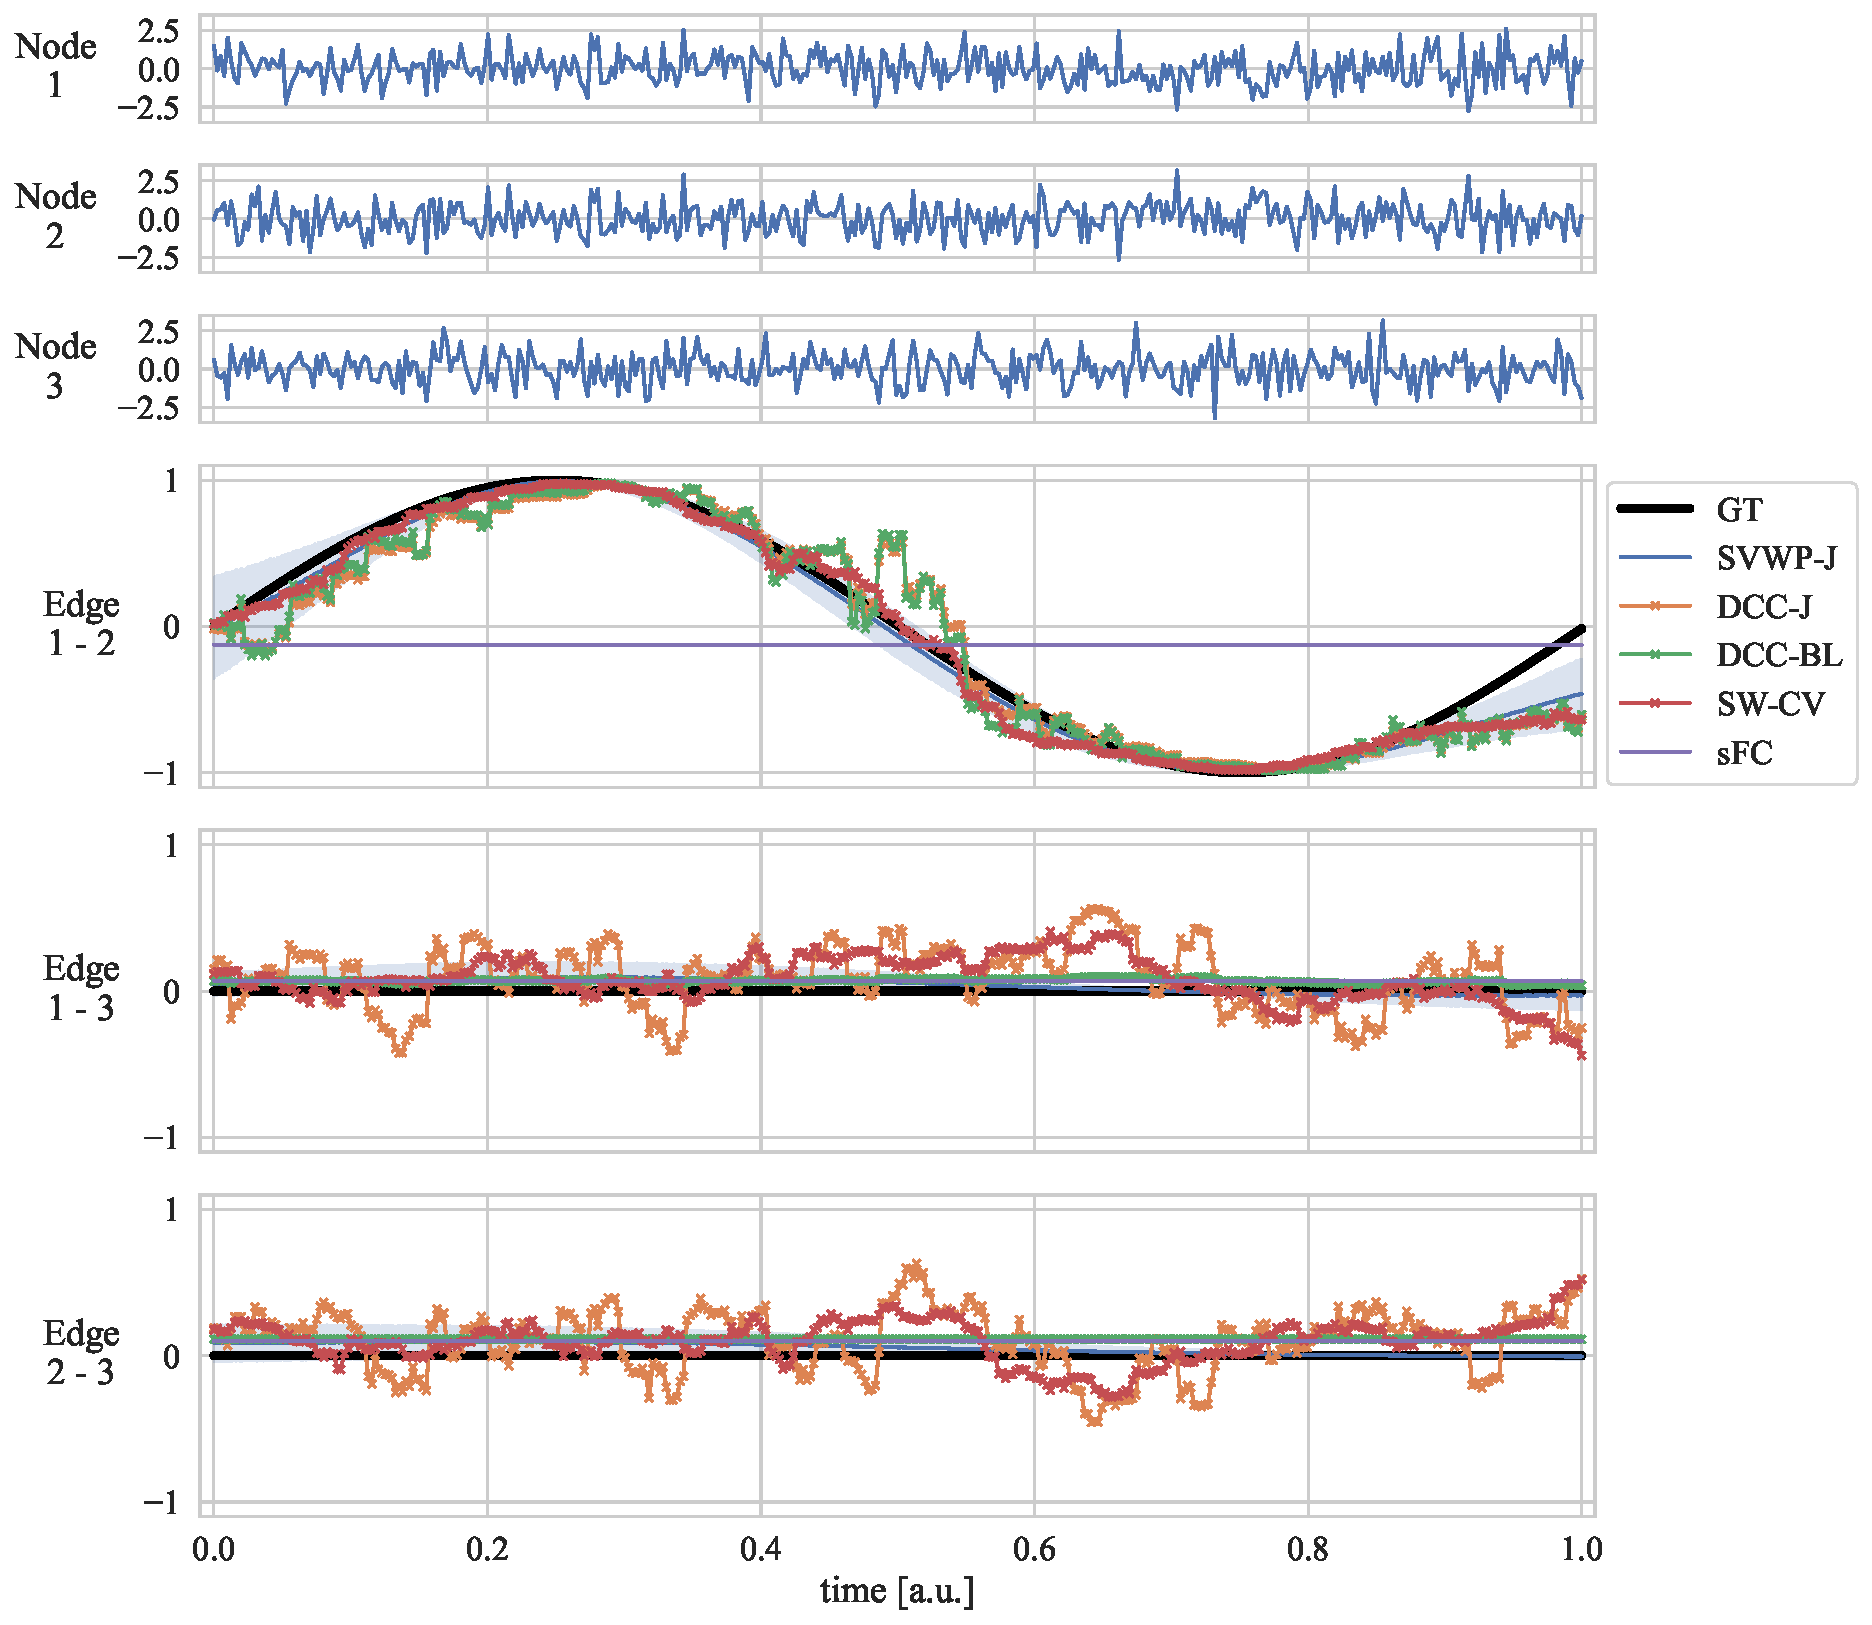
\includegraphics[width=\textwidth]{fig/sim/d3s/N0400_T0003/no_noise/periodic_1_correlations}
  \caption{
    Demonstration and motivation for training models in pairwise fashion when edges are characterized by radically different covariance structures.
  }
  \label{fig:pairwise-vs-joint}
\end{figure}


\info[inline]{Paragraph: Discuss our approach to this issue.}
In a theoretical approach, in general, a model should expect to always find some pair that seems correlated when presented with a large number of pairs.
A multivariate model would not extract spurious structure if it only sees one odd case out of many, or at least would need even more evidence.
However, the pairwise approach would not have this inherent protection against reporting false positives.
Of course, such issues could be resolved through careful post-estimation multiple comparison correction.
%
On the other hand, in an empirical approach, we can also directly compare both implementations (joint and pairwise loop) and check which one performs better on the benchmarks.
In fact, this is one of the strengths of properly designed benchmarks: it reduces speculation.
For example, \cref{fig:pairwise-vs-joint} shows \gls{tvfc} estimates for a toy example of $D = 3$ simulated time series, where the first two nodes exhibit a periodic covariance structure and the other edges are uncorrelated.
The pairwise \gls{dcc} model predicts better than the jointly trained \gls{dcc} model, arguably because the covariance structure characteristics are radically different for the different edges.
This seems to motivate the benefit of training \gls{dcc} in a pairwise fashion.
However, as we shall see later, in realistic scenarios these differences will not be as pronounced, and the two ways of training yield very similar estimates.
%
Throughout this thesis we train all models in joint fashion, except \gls{dcc} which will be trained in both manners.
The `-J' suffix will indicate a multivariate jointly trained model, where `-BL' will refer to bivariate (pairwise) loop training.
For the bivariate case, this distinction becomes meaningless, and the suffixes are dropped.

%%
\subsection{Autoregressive and full process dependence}
%%

Estimation methods can broadly be divided into constructions that are autoregressive (taking only past observations into account) in nature or that depend on the full process.
%
\Glspl{gp} assume full process dependence, so our \gls{wp} follows suite.
Methods based on \gls{sw} fall into this category as well.
%
However, the \gls{dcc} method does not, and in their introductory paper \textcite{Lindquist2014} designed their \gls{sw} methods to only incorporate past data to allow for a fair comparison.
Training \gls{dcc} models does involve tuning hyperparameters, however, which are learned based on the full time series.
%
In this thesis we argue that forecasting is typically not of major interest in neuroimaging, and that full scans are always available at analysis time.
Therefore, we do not make a distinction between such models, and compare them head-to-head.

%%
\subsection{Beyond simple performance metrics}
%%

\info[inline]{Paragraph: Discuss other key motivations when choosing a TVFC estimation method.}
While a carefully designed benchmark and performance metric should provide guidance on what methods perform best, there are other method qualities that are desirable.
%
These include computational complexity, uncertainty modeling and estimation, robustness, ease of implementation, explainability, and flexibility in general.
%
These will be considered secondary (or \emph{auxiliary}) factors in our model comparison.
For example, it seems reasonable to want to sacrifice on performance slightly if it would get you many other attractive characteristics in return.
%
We will return to this in \cref{ch:discussion}.

%%
\subsection{Other benchmarks}
%%

\info[inline]{Paragraph: Discuss other benchmarks not included here and what we miss out on.}
The families of benchmarks discussed in this chapter are not exhaustive.
%
Other benchmarks outside the scope of this thesis include predicting a concurrent modality.
For example, by using a simultaneous \gls{fmri}-\gls{eeg} data set~\parencite{Laufs2003}.
\textcite{Tagliazucchi2014} predicted sleep state from \gls{fmri} using such a concurrent data set.
Other concurrent modalities are possible as well.
For example, \textcite{Matsui2016} simultaneously monitored neuronal calcium signals and \gls{fmri}.
%
The problem with such data sets is often that they are hard to process and understand, and they may not make for practically useful benchmarking data sets at the moment.
This leads to typically sample sizes too.

%%
\chapter{Benchmarking TVFC estimation}
\label{ch:benchmarking}
%%%%%

\info[inline]{Paragraph: Introduce benchmarking chapter.}
In this chapter we describe the benchmarks studied and compare the \gls{tvfc} estimation methods described in \cref{ch:methods}.
We start with simulations-based benchmarks and then move on to benchmarks based on real data, both \gls{rs-fmri} and \gls{tb-fmri}.
The simulations allow for flexibility and the testing of edge cases.
Moving to real data constitutes a step toward a practical, realistic application of \gls{tvfc} estimation.
Since we lack a ground truth (i.e.~target variable) in these latter benchmarks, we will look at how to choose or design \emph{proxies} for it.
The same \gls{tvfc} estimation methods are investigated for all benchmarks in this chapter.
Adding methods to the benchmarking framework should be reasonably easy, and all required code will be made available upon publishing.

\clearpage
\section{Material and methods}\label{sec:simulations-methodology}
%%%%%

In this section we describe the respective benchmarks and related methodology in detail.

%%
\subsection{Simulations}\label{subsec:simulations-methods}
%%

We consider a range of simulation studies with various deterministic synthetic covariance structures.
We take full advantage of the flexibility that simulations offer, and explore a wide range of data (e.g.~dimensionalities and noise configurations) and estimation method (e.g.~hyperparameters and post-hoc analysis) characteristics.
The synthetic covariance structures are both designed for exploring edge cases as well as mimicking structures that we may expect to drive actual processes in the human brain.

%%
\subsubsection{Synthetic covariance structures}\label{subsec:synthetic-covariance-structures}
%%

Perhaps surprisingly, the covariance structures to be expected in real data are rarely discussed.
The coupling of \gls{bold} time series is, in fact, still a black box to a large degree.
In lieu of known covariance structure we test models against a battery of possible and reasonably exhaustive (synthetic) structures that may be encountered in an \gls{fmri} scan.
The covariance structures studied are shown in \cref{fig:synthetic-covariance-structures};
null covariance (node time series are uncorrelated during the entire scan)\improvement{Discuss importance of adding null model},
a constant (i.e.~static) covariance of $\sigma_{ij} = 0.8$,
periodic covariance structures (a slowly oscillating sine wave defined by one period, and a fast one with three periods) that model transient changes in coupling,
a stepwise covariance that models two sudden (large) change points in covariance,
a covariance structure that simulates a series of state transitions, as inspired by~\textcite{Thompson2018},
and finally a covariance structure inspired by the \gls{tb-fmri} visual checkerboard task we study (see \cref{subsec:rockland-methodology}).
This last covariance structure mimics the presence and absence of an external visual stimulus (assuming it would show up as such in the covariance structure).
It is designed by taking the convolution between the \gls{hrf} and the respective stimulus block design.


\begin{figure}[t]
  \centering
  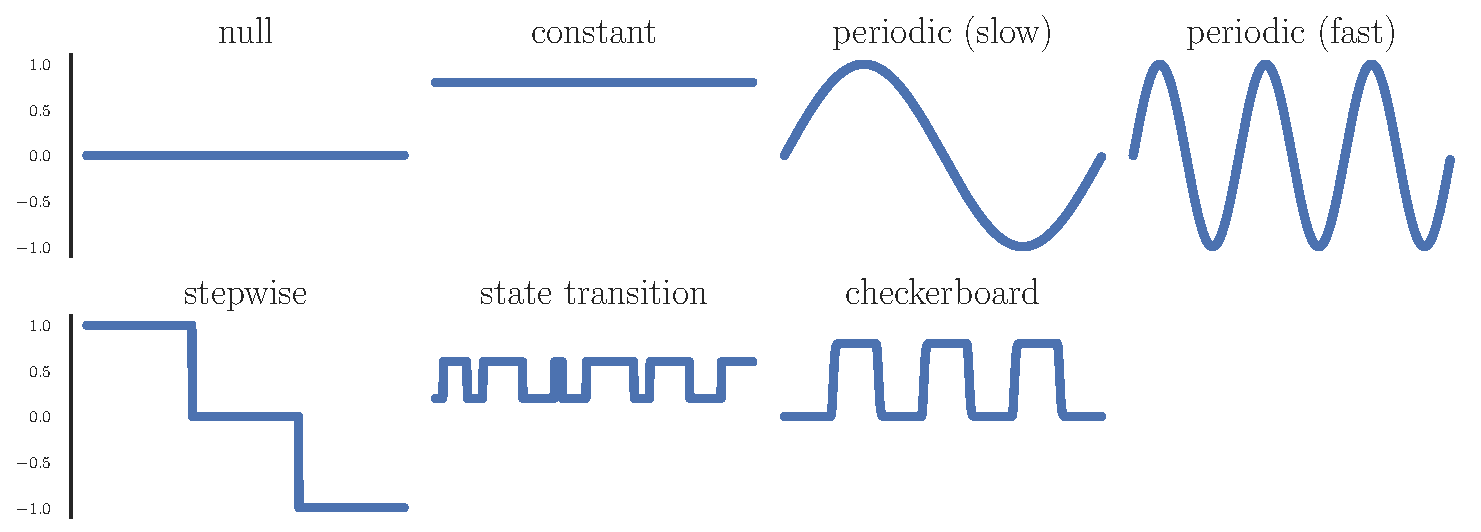
\includegraphics[width=\textwidth]{fig/sim/covariance_structures}
  \caption{
    Synthetic covariance structures as a function of time considered in the simulations benchmark.
    These capture a wide range of edge cases and potentially realistic underlying covariance structures that generate the observed node time series.
  }\label{fig:synthetic-covariance-structures}
\end{figure}


%%
\subsubsection{Data generation}
%%

Data is simulated as follows.
We sample observations $\mathbf{y}_n \in \mathbb{R}^D$ at each time step~$1 \leq n \leq N$ from a zero-mean Gaussian distribution:
\begin{equation}
  \mathbf{y}_n \sim \mathcal{N}(\mathbf{0}, \mathbf{\Sigma}_n),
  \label{eq:data-generation}
\end{equation}
for a given covariance matrix $\mathbf{\Sigma}_n$ at time step $n$.
This covariance matrix depends on the synthetic covariance structure parameters defining the data set.
All time series are subsequently individually normalized to have mean zero and unit standard deviation.

The number of time series ($D$) we expect to see in practice depends on the experimental design and research question at hand.
In most applications more than two nodes or components are studied.
Some studies even consider voxel time series directly, in which case $D$ can be in the hundreds of thousands.
Here, we test on pairwise (i.e.~\emph{bivariate}; $D = 2$) data, as well as on a trivariate ($D = 3$) data sets.
Ideally, we want to study \gls{tvfc} estimation performance per method \emph{as a function of} dimensionality.
The trivariate case serves as an intermediate step toward scaling up to higher dimensions.
All simulation experiments are repeated $T = 200$ times to ensure robustness while balancing computational cost.
Model performance is averaged across these trials.

The bivariate benchmark analyses are similar to the ones conducted by~\textcite{Lindquist2014}.
Furthermore, they will serve as a blueprint for when we analyze connectivity between just two brain regions.
It is important to note that methods based on \gls{sw} are always pairwise as well.
Thus, if a method robustly and consistently outperforms \gls{sw} on bivariate data, it will do so on higher dimensional data as well if we were to simply loop over all pairs of time series.

The covariance structure in \cref{eq:data-generation} for generating bivariate data is given by
\begin{equation}
  \mathbf{\Sigma}_n = \begin{bmatrix}
    1 & \sigma(n) \\
    \sigma(n) & 1
  \end{bmatrix},
\end{equation}
where the covariance term $\sigma(n)$ varies across time according to the various covariance structures shown in \cref{fig:synthetic-covariance-structures}.
For the bivariate case, $\sigma(n)$ is allowed to fall within range~[-1,1], to maintain a positive semi-definite matrix.
As mentioned before, since the diagonal consists of ones, these covariance matrices are identical to their respective correlation matrices.

For the trivariate data, we implement both a fully co-varying (i.e.~\emph{dense}) covariance structure
\begin{equation}
  \mathbf{\Sigma}_n = \begin{bmatrix}
    1 & \sigma(n) & \sigma(n) \\
    \sigma(n) & 1 & \sigma(n) \\
    \sigma(n) & \sigma(n) & 1
  \end{bmatrix},
\end{equation}
and a \emph{sparse} version where only the first two time series are correlated
\begin{equation}
  \mathbf{\Sigma}_n = \begin{bmatrix}
    1 & \sigma(n) & 0 \\
    \sigma(n) & 1 & 0 \\
    0 & 0 & 1
  \end{bmatrix},
\end{equation}
where the covariance terms $\sigma(n)$ again vary across time as depicted in \cref{fig:synthetic-covariance-structures}.
This sparse version can be considered alike to the bivariate case with an added uncorrelated (i.e.~control) region.
Perhaps we would expect such structure (most edges being stationary, but some showing time-varying structure) in \gls{fmri} data.
Yet, lacking a ground truth again makes this unclear.
To keep the covariance matrices positive semi-definite, the allowed range for $\sigma(n)$ in the dense trivariate case is~$[-0.5,1]$ while for the sparse version it remains~$[-1,1]$.

We want our results to be robust across data set lengths.
\gls{fmri} scans (whether \gls{rs-fmri} or \gls{tb-fmri}) are typically in the order of~240 to~1,200 seconds; participants can only be kept in a scanner for a limited amount of time.
The \gls{tr} of scanning setups typically ranges from~0.5 to~2 seconds.
Combining these ranges gives us a range of the number of data points $N$ we expect to see in practice.
Therefore, we study the cases of $N \in \{120, 200, 400, 1200\}$ data points per time series.
We report results for $N = 400$, because this is the closest to the values of $N$ in \cref{ch:ukb} and thus most representative.
Results for other values of $N$ are retired to \cref{appendix:more-benchmarking-results}.
It is important to be aware of the typical trade-off where scans with higher \glspl{tr} consist of fewer data points, although the increase in number of slices per scanning volume can result in higher spatial resolution and reduce autocorrelation effects and other sources of noise~\parencite{Amaro2006, Iranpour2015, Yoo2018, McDowell2019}.
We also note that Bayesian methods typically perform better on smaller data sets.
Even though we strive to find a robust method that can be used in any setting, we consider the option that some methods may work better with smaller but less noisy data sets and other methods may perform better with larger, noisy data sets.
This style of analysis is reminiscent of the multiverse analysis~\parencite{Steegen2016}, as discussed in more detail in \cref{subsec:robustness}.

%%
\subsubsection{Noise addition and hybrid simulations}
%%

The human nervous system is subject to various sources of noise, such as Brownian motion in synapses and ion channels~\parencite{Faisal2008}.
\gls{fmri} scanners are imperfect machines and introduce further sources of noise as well.
These account for system noise and observational noise.
Taken together this makes \gls{fmri} data (in)famously noisy~\parencite[see also][for analysis and biophysical simulations of impact of noise and delay]{Deco2009}.
The noise is both spatially and temporally correlated.

To make our benchmark more robust, all experiments are repeated on the data sets described above, but with added noise.
Noise ensures generalizability of any conclusion we make.
Higher levels of noise can also be interpreted as decreasing the amplitude of any existing covariance structure, requiring methods to be increasingly sensitive.
In an extensive literature review, \textcite{Welvaert2013} found \gls{snr} values in \gls{fmri} data to range between 0.35 and 203.6.
Higher \glspl{snr} are preferred in practice.
%
Here, all experiments are repeated with added noise with an \gls{snr} $\in \{1, 2, 6\}$.
Empirically, we found that any lower \gls{snr} causes all \gls{tvfc} estimation methods to break down, and any higher \gls{snr} yields results equivalent to the noiseless case.

Two types of added noise are studied.
The simplest case (white noise) can be considered like thermal noise in \gls{fmri} scanners.
\unsure{Do we still want to report the white noise results?}
Secondly, in the \emph{hybrid} simulations, we use an \gls{rs-fmri} data set to add noise to the synthetically generated activation data.
We use data from the \gls{hcp} data set as described in more detail in \cref{subsec:data-hcp}.
If we take time series from brain regions (or \gls{ica} components) from different subjects and add them to the synthetic signal, we can assume that no additional covariance structure is added.
These \gls{rs-fmri} time series are selected from the middle of the scans.
Such hybrid simulations are similar in spirit to \textcite{Keilholz2013}, where subject scan session IDs are randomized to ensure a proper null model for a statistical test.
The benefit of this is that we preserve typical \gls{fmri} time series characteristics.
For \gls{rs-fmri} data this typically includes heavy spatial and temporal autocorrelation~\parencite{Keilholz2017}, which has been shown to affect \gls{tvfc} estimates~\parencite{Honari2019}.
This is contrasted to \textcite{Thompson2018}, where autocorrelation is specified and simulated in the data directly.
We argue that since we do not know what a realistic level of autocorrelation would be, using real data autocorrelation is preferred.

In both noise addition routines, we consider our noisy $\mathbf{y}_n^*$ to be a linear mix of noiseless signal $\mathbf{y}_n$ (as defined above) and (independent) noise time series $\mathbf{\epsilon}_n$:
\begin{equation}
  \mathbf{y}_n^* = \alpha \mathbf{y}_n + (1 - \alpha) \mathbf{\epsilon}_n,
\end{equation}
where $0 < \alpha < 1$ is called the mixing coefficient, with the \gls{snr} being equal to $\frac{\alpha}{1-\alpha}$.

Adding noise affects the signal (ground truth) variances and covariances.
The time series variances and covariances are updated as follows.

In the case of white noise, $\mathbf{\epsilon}_n \sim \mathcal{N}(\mathbf{0}, \mathbf{I})$.
To understand what will happen to the variances of each time series, we firstly note that
\begin{equation}
  \mathbb{E}[\mathbf{y}_n^*] = \alpha \mathbb{E}[\mathbf{y}_n] + (1-\alpha)\mathbb{E}[\mathbf{\epsilon}_n] = \mathbf{0}.
\end{equation}
This means that the new time series variance is
\begin{equation}
  \begin{split}
    \sigma_{y_n^*}^2 & = \mathbb{E}[(\mathbf{y}_n^*)^2] - (\mathbb{E}[\mathbf{y}_n^*])^2 = \mathbb{E}[(\mathbf{y}_n^*)^2] \\
    & = \mathbb{E}[\alpha^2 \mathbf{y}_n^2 + 2\alpha(1-\alpha)y_n\mathbf{\epsilon}_n + (1-\alpha)^2\mathbf{\epsilon}_n^2] \\
    & = \alpha^2\mathbb{E}[\mathbf{y}_n^2] + (1-\alpha)^2\mathbb{E}[\mathbf{\epsilon}_n^2] \\
    & = \alpha^2 + (1-\alpha)^2.
  \end{split}
\end{equation}
Regarding the covariance terms, all cross-terms except within $\mathbf{y}_n$ are zero, so we are simply left with $\sigma_{y_{n,1}^*y_{n,2}^*} = \alpha^2\sigma_{y_{n,1}y_{n,2}}$.
To maintain the time series variances $\sigma_{y_t^*}^2$ being equal to 1, we compute the new (noisy) signal as given by
\begin{equation}
  \mathbf{y}_n^* = \frac{1}{\sqrt{\alpha^2 + (1-\alpha)^2}} [\alpha \mathbf{y}_n + (1 - \alpha) \mathbf{\epsilon}_n],
\end{equation}
so that our new ``ground truth'' covariance terms are updated as
\begin{equation}
  \sigma_{y_{n,1}^*y_{n,2}^*} = \frac{\alpha^2}{\alpha^2 + (1-\alpha)^2} \sigma_{y_{n,1}y_{n,2}}.
\end{equation}

In the hybrid experiments, we adjust the ground truth covariances in the same way as with white noise.
Although the distribution of the noise is not known, we know that $\mathbb{E}[\epsilon] = 0$ and $\mathbb{E}[\epsilon^2] = 1$, since we normalized it as such.

%%
\subsubsection{Evaluation and performance metrics}
%%

Comparing model estimates visually provides an initial overview of method performance and qualitative characteristics.
To \emph{quantify} performance, we compute the \gls{rmse} between estimated and ground truth Pearson correlation, following~\textcite{Wilson2010, Lindquist2014}.
This can be considered a \emph{reconstruction} loss.
Estimators with lower \gls{rmse} will be considered superior estimators.
For the trivariate cases, we compute the \gls{rmse} across all elements of the full correlation matrices.

%%
\subsubsection{Imputation benchmark}
%%

The imputation benchmark is run as described in \cref{subsec:imputation-benchmark}.
Of course, it is unnecessary to do so because we have the actual underlying ground truth.
However, this allows us to investigate the relationship between method performance on this imputation benchmark and its ability to recover an actual ground truth.

%%
\subsection{Resting-state fMRI}
%%

\info[inline]{Paragraph: Introduce rs-fMRI-based benchmarks.}
Here we study how an \gls{rs-fmri} data set can be used to benchmark \gls{tvfc} estimation methods.
We look at different (common) classes of benchmarks based on \gls{rs-fmri} data: the prediction of subject measures, test-retest robustness, and the imputation benchmark as described in \cref{subsec:imputation-benchmark}.
For the latter we are especially interested in its relationship with the other benchmarks.
We use a single source of data for all these \gls{rs-fmri} benchmarks: the \gls{hcp}.
Moreover, we conduct a brain state analysis.
This analysis is more suited as demonstration rather than benchmark.

%%
\subsubsection{Data: Human Connectome Project}\label{subsec:data-hcp}
%%

The \gls{hcp} has collected a large, publicly available data set collected in 2012--2015.\footnote{Data: \url{https://www.humanconnectome.org}}
It is one of the largest and most used data sets in neuroimaging research~\parencite{VanEssen2012, VanEssen2013, Elam2021}.
It is important to use publicly available and transparently collected data to benchmark methods.
Participants in this data set are relatively young adults (twins and non-twin siblings), aged 22--35.
The data collection and collaboration of this project were accompanied by fundamental technological advances underlying scan collection.
This included advances in the domains of accelerated multiband and multiplexed \gls{epi} pulse sequences~\parencite{Moeller2010, Feinberg2010, Setsompop2012, Xu2012}.
The data is accompanied by a range of behavioral and non-behavioral subject measures (many of these collected through the NIH toolbox).

More specifically, we use data from the \gls{hcp} S1200 public release (published in March 2017).
This (final) release contains 1,113 subjects with \gls{mri} data.
Of these, 1,003 subjects have complete (i.e.~four scans) \gls{fmri} data available.
However, only 812 subjects with improved \gls{fmri} image reconstruction (\texttt{recon2}) are available.
We use data from these 812 subjects only.
All scans are acquired with a 3T Siemens connectome-Skyra using a multi-band sequence.
%
The readily available $D = 15$ dimensional \gls{ica} based node time series are used.
\Gls{ica} is a technique that decomposes observed (voxel) time series into a set of independent components.
The original individual observed time series can then be reconstructed as a mix of these components.
Each of these \gls{ica} time series thus represents a significant \emph{component} of whole-brain activity.
Other dimensionalities $D \in \{25,50,100,200,300\}$ are also readily available.
However, we opted to study $D = 15$ time series, as this number of time series is most representative of the number studied in many cognitive studies, including the ones in this thesis.
For example, the depression study in \cref{ch:ukb} studies both nine and three time series.
%
For interpretability, each \gls{ica} component is mapped to a well-known \gls{fn}, following \textcite{Giorgio2018}.
We asked three neuroimaging researchers to visually inspect and manually assign each \gls{ica} component to one of the networks from \cref{fig:brainmap-functional-networks}; networks that resemble task-driven \glspl{fn}~\parencite{Fox2007, Smith2009}.


% Remove (a), (b), etc.
\captionsetup[subfigure]{labelformat=empty}

\begin{figure}[t]
  \centering
  \subcaptionbox{1: Visual (Medial)\label{fig:rsn-1}}{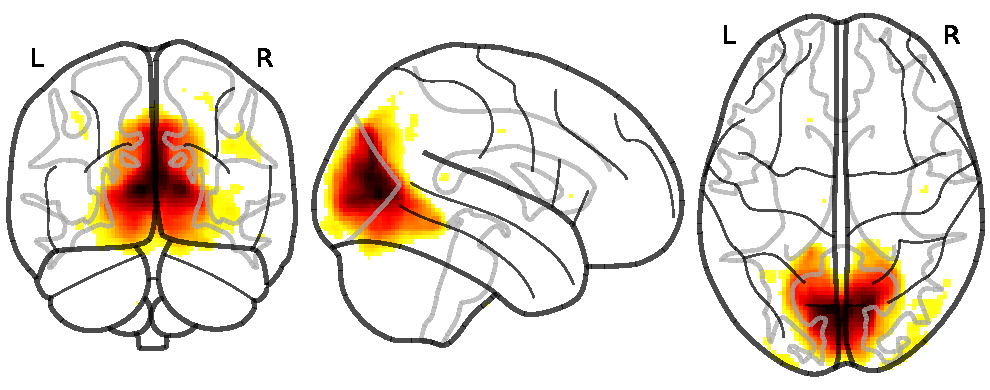
\includegraphics[width=0.38\textwidth]{fig/hcp/RSN_components/RSN_00}}
  \hspace{0.08\textwidth}
  \subcaptionbox{2: Visual (Occipital, Cognition-Language-Orthography)\label{fig:rsn-2}}{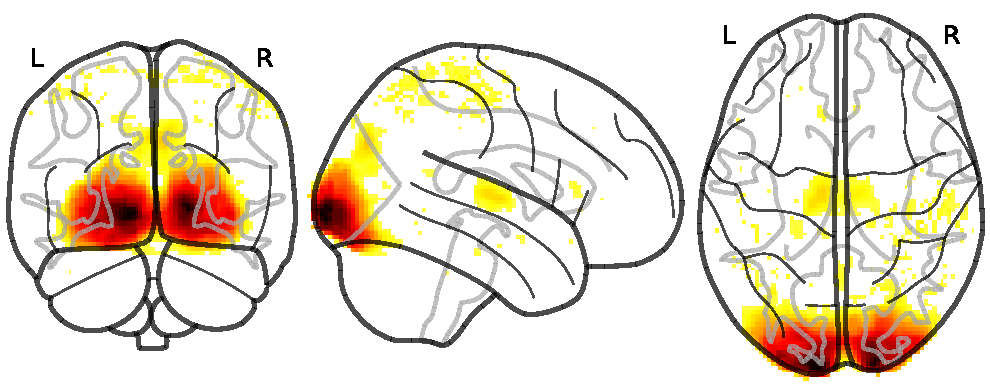
\includegraphics[width=0.38\textwidth]{fig/hcp/RSN_components/RSN_01}}
  \subcaptionbox{3: Visual (Lateral, Cognition-Space)\label{fig:rsn-3}}{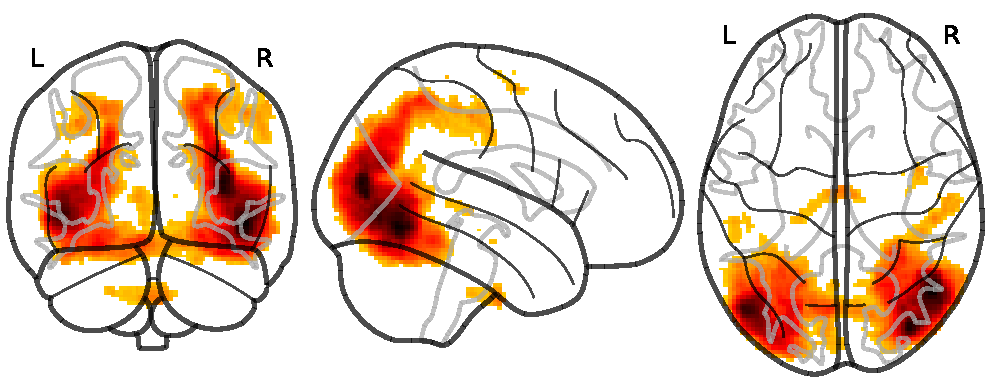
\includegraphics[width=0.38\textwidth]{fig/hcp/RSN_components/RSN_02}}
  \hspace{0.08\textwidth}
  \subcaptionbox{4: Default Mode Network (DMN)\label{fig:rsn-4}}{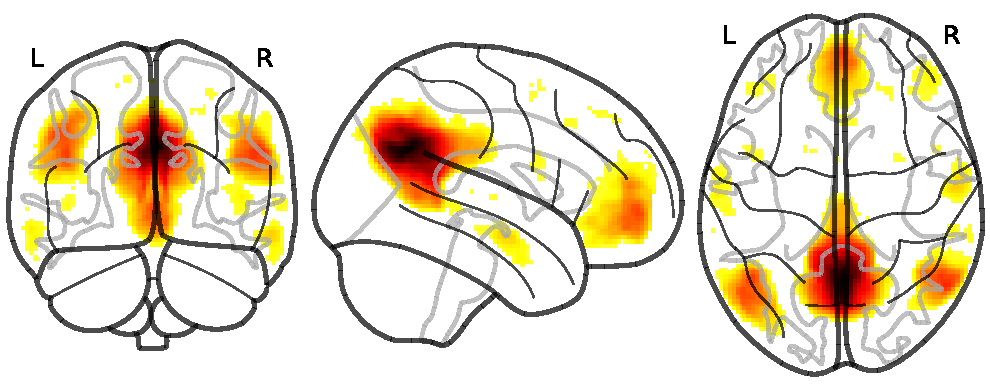
\includegraphics[width=0.38\textwidth]{fig/hcp/RSN_components/RSN_03}}
  \subcaptionbox{5: Cerebellum (CBM)\label{fig:rsn-5}}{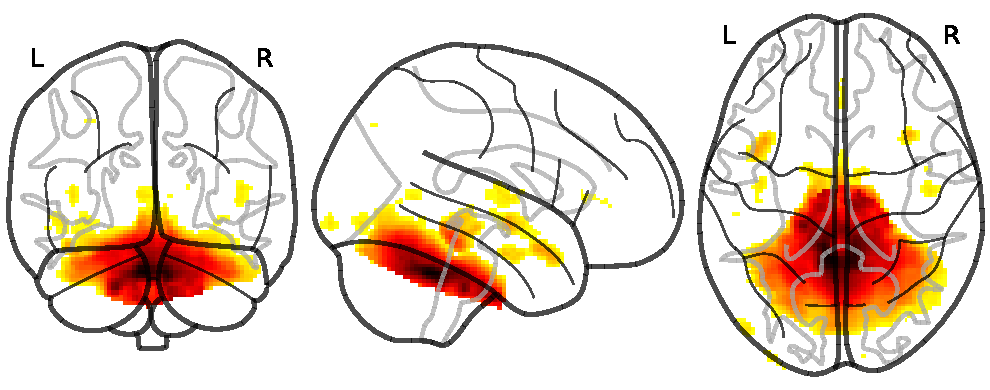
\includegraphics[width=0.38\textwidth]{fig/hcp/RSN_components/RSN_04}}
  \hspace{0.08\textwidth}
  \subcaptionbox{6: Sensorimotor (SM)\label{fig:rsn-6}}{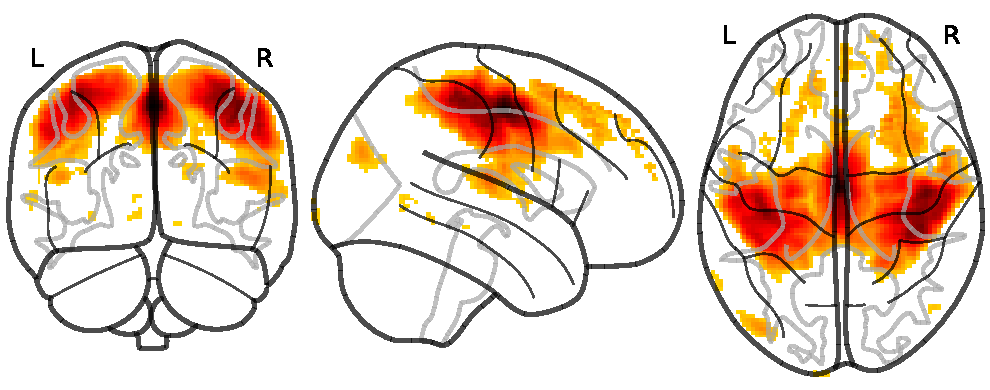
\includegraphics[width=0.38\textwidth]{fig/hcp/RSN_components/RSN_05}}
  \subcaptionbox{7: Auditory (AUD)\label{fig:rsn-7}}{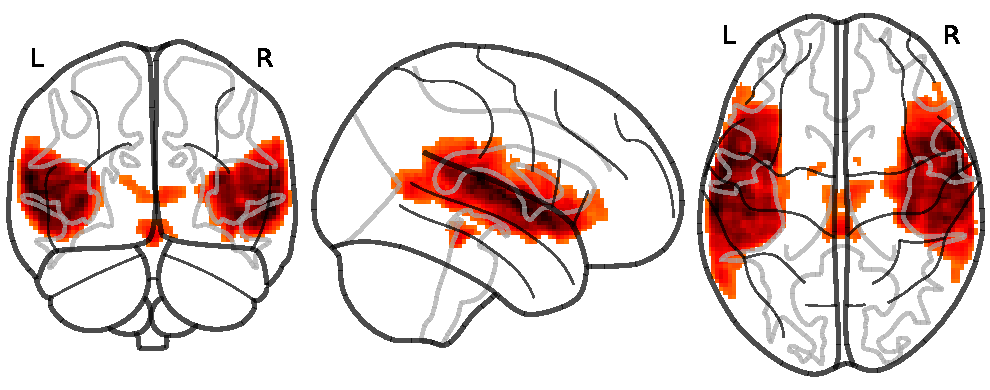
\includegraphics[width=0.38\textwidth]{fig/hcp/RSN_components/RSN_06}}
  \hspace{0.08\textwidth}
  \subcaptionbox{8: Executive Control (EC)\label{fig:rsn-8}}{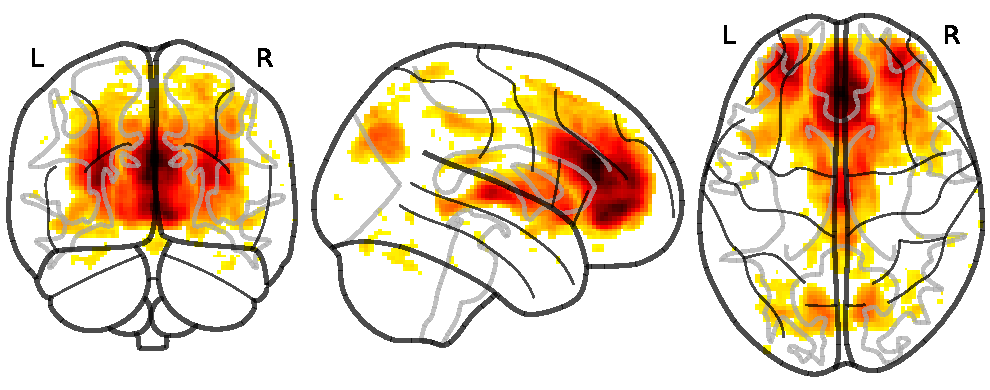
\includegraphics[width=0.38\textwidth]{fig/hcp/RSN_components/RSN_07}}
  \subcaptionbox{9: Frontoparietal (Perception-Somesthesis-Pain)\label{fig:rsn-9}}{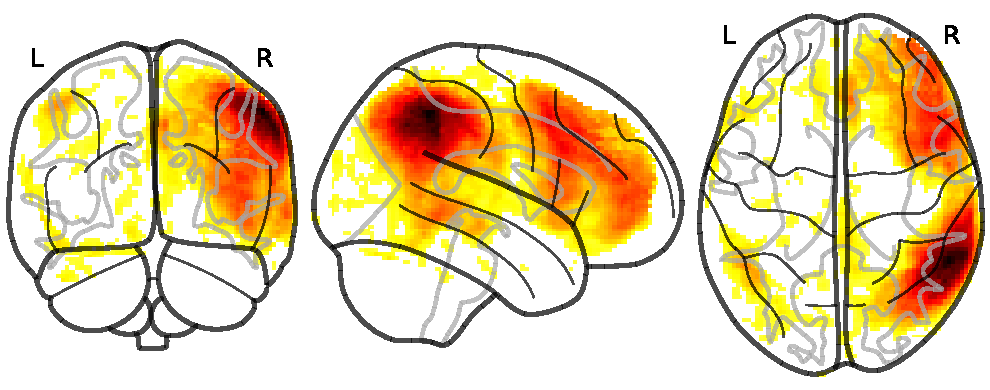
\includegraphics[width=0.38\textwidth]{fig/hcp/RSN_components/RSN_08}}
  \hspace{0.08\textwidth}
  \subcaptionbox{10: Frontoparietal (Cognition-Language)\label{fig:rsn-10}}{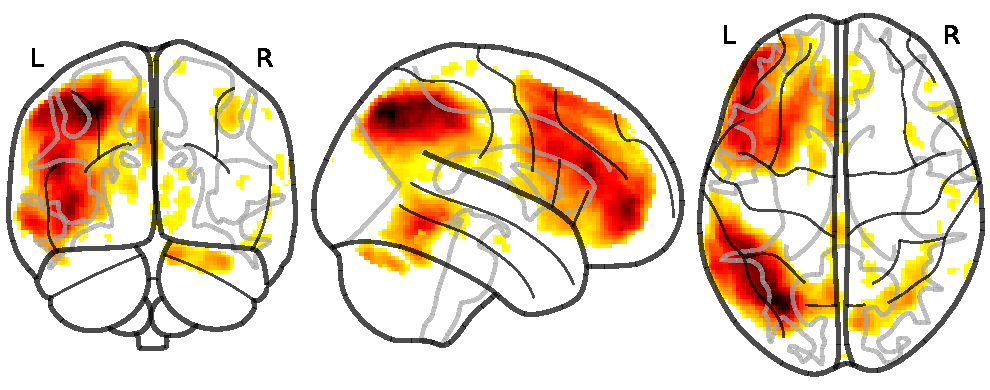
\includegraphics[width=0.38\textwidth]{fig/hcp/RSN_components/RSN_09}}
  \caption{
    Functional networks from \textcite{Smith2009}.
  }\label{fig:brainmap-functional-networks}
\end{figure}

% Add back (a), (b), etc.
\captionsetup[subfigure]{labelformat=parens}


Each subject undergoes four scans in total, divided into two consecutive scans on two separate days.
We will refer to these scans as 1A, 1B, 2A, and 2B.
We only include subjects for which all of these four scans are available, resulting in 812 subjects in total.
Scans were acquired with a \gls{tr} of 0.72 seconds and voxel size of 2~mm isotropic.
Each scan contains $N = 1200$ images and is 15 minutes long.
%
Data was preprocessed by the \gls{hcp} team according to \textcite{Smith2013a} with a (minimal) preprocessing pipeline using \gls{fsl}~\parencite{Jenkinson2012} and FreeSurfer~\parencite{Fischl2012}.
The pipeline is described in more detail in \textcite{Jenkinson2002, Glasser2013, Smith2013b}.
Importantly, noise components have been filtered out during preprocessing using \gls{ica}+FIX~\parencite{Salimi2014, Griffanti2014}.
This ensured that none of the components we use can be considered as a noise component.
All time series were also demeaned, with variance normalized~\parencite{Beckmann2004}.
All \gls{ica} components for each subject and for each scan were individually standardized to have zero mean and unit variance.
For more data preprocessing details, we refer the reader to the \gls{hcp} release manual.

%%
\subsubsection{Subject measure prediction benchmark}
%%

One common benchmarking approach is to investigate the predictive power of subject measures (i.e.~phenotypes, such as subject age) from \gls{tvfc} estimates from the different methods, using regressors and classifiers.
This makes sense on multiple levels.
We know that individual differences are contained in \gls{rs-fmri} scans~\parencite{Finn2015}.
Furthermore, subject measure prediction is similar to many practical use cases of \gls{tvfc} estimates, for example when used in clinical contexts for disease diagnosis and prognosis.
%
The idea here is as follows.
If a method's estimated covariance structure has more predictive power than another's, it can be said it has extracted and preserved more relevant information (for the prediction task at hand).
It is likely that some methods preserve more relevant information for some tasks, yet other methods preserve more for other tasks.
However, we can look at the average across many subject measures, or we may suggest which method to use after selecting a subject measure of interest.
As such this benchmarking can be considered a `profiling' or `cataloging' exercise.
Here we investigate the task of predicting subject measures for subjects from the \gls{hcp} data set.

\info[inline]{Paragraph: Describe morphometricity algorithm.}
Estimated covariance structure and subject measures are related through a \textbf{morphometricity} analysis~\parencite{Sabuncu2016}, using the variance component model.
This model, based on \gls{lme} modeling, finds a linear relationship between estimated \gls{tvfc} and subject measures.
\textcite{Sabuncu2016} defined this global metric of morphometricity as the proportion of phenotypic variation that can be explained by macroscopic brain morphology (i.e.~inter-subject anatomical variation).
The score has a value between 0 and 1, with 1 explaining all variance.
Their original study looked at anatomical variation between subjects.
Therefore, in their context this score is a measure of the anatomical signature of a certain trait.

Scores are computed as follows.
We posit for following model:
\begin{equation}
  \mathbf{y} = \mathbf{X} \mathbf{\beta} + \mathbf{a} + \mathbf{\epsilon},
  \label{eq:lme}
\end{equation}
where $\mathbf{y}$ is a column vector of length equal to the number of subjects studied containing, some quantitative subject measure (e.g.~age), $\mathbf{X}$ is the design matrix of confounding variables (a.k.a.~covariates or nuisance variables) weighted by~$\mathbf{\beta}$, $\mathbf{a}\sim \mathcal{N}(\mathbf{0}, \sigma_a^2 \mathbf{K}_a)$ is a random effects vector, and $\mathbf{\epsilon} \sim \mathcal{N}(\mathbf{0}, \sigma_e^2)$ is a noise vector.
We call the symmetric matrix $\mathbf{K}_a$ the \gls{tvfc} similarity matrix (in contrast with the original paper, where it is called the \emph{anatomical} similarity matrix).
Each value in this matrix encodes how globally `similar' two subjects are.
It is still our choice how to define similarity in this case based on \gls{tvfc} estimates.
More specifically then, morphometricity is computed as
\begin{equation}
  m^2 = \frac{\sigma_a^2}{\sigma_a^2 + \sigma_e^2} = \frac{\sigma_a^2}{\sigma_y^2},
\end{equation}
where $\sigma_y^2$ is called the phenotypic variance.
In order words, morphometricity is the amount of phenotypic variation that can be explained by variation in \gls{tvfc} estimates.
Parameters~$\sigma_a^2$ and~$\sigma_e^2$ are estimated using the \gls{reml} method~\parencite{Patterson1971, Harville1977}.
We can use this in our model comparison framework as follows: methods whose \gls{tvfc} estimates can explain more subject phenotypic variation can be considered superior.

\info[inline]{Paragraph: Define subject-by-subject similarity matrix.}
How should we define the similarity $\mathbf{K}_a$ between subjects?
In our analysis we re-purpose the morphometricity analysis and consider subject `similarity' as indicated by whole-brain estimated \gls{tvfc}.
Instead of using the full $N \times D \times D$ estimated covariance structure, we use the $D \times D$ dimensional summary measures of it.
The summary measures are the mean, variance, and rate-of-change of \gls{tvfc} estimates, as discussed in \cref{subsec:tvfc-summary-measures}.
This can be viewed as a feature or biomarker extraction step.
We take the lower triangular values as a vector of size $\frac{D(D-1)}{2}$, excluding the diagonal (self-connections) and duplicate values (since the matrices are symmetric).
Following \textcite{Sabuncu2016}, distance between subjects is defined by a Gaussian kernel, that is $k(\textbf{x}, \textbf{x}') = \exp(-(x-x')^2)$.

\info[inline]{Paragraph: Describe our subject measures.}
The variance component model relates \gls{tvfc} estimates to just a single phenotype or subject measure.
We repeat the analysis for a range of subject measures.
%
In fact, another study has run a similar analysis to benchmark \gls{fmri} data preprocessing.
In this work, \textcite{Li2019a} studied the predictive power of \gls{sfc} estimates after both including or excluding a crucial preprocessing pipeline researcher choice: whether to include \gls{gsr} or not.\footnote{The respective authors also implemented a regression on top of this. They found that the predictive power and the amount of variance explained are highly correlated concepts.}
They conclude that \gls{gsr} significantly increases the predictive power of \gls{sfc} estimates.
To allow for comparison and because they capture a wide range of individual differences, we study the exact same behavioral subject measures as they did: age, gender, and a range of cognitive task scores.
These subject measures were investigated in a related study as well~\parencite{Kong2019}, where it was found that not only \gls{sfc} but also network topography has predictive power of such measures.
%
Age and gender are included as nuisance variables in our model, that is $\mathbf{X}$ in \cref{eq:lme}.
Some subject measures were missing from the raw data.
We filled missing values with mean imputation.
%
Furthermore, the same analysis is run on social-emotional and a range of other subject measures (including personality).
However, these are considered as less relevant, and their results have been moved to \cref{appendix:hcp-more-results}.

%%
\subsubsection{Test-retest robustness benchmark}
%%

Apart from a performance metric that captures how well methods can estimate covariance structures, we can also compare method \emph{robustness} across scans from the same subject.
Such robustness is another desired property of any \gls{tvfc} estimation method.
The idea here is that a method that predicts consistent subject attributes across scans should be more robust and would have captured some aspect of individual differences.

Here we broadly follow \textcite{Choe2017} and their test-retest study for \gls{tvfc} estimates in \gls{rs-fmri} data.
They studied the same data set, albeit an older and smaller version thereof.
%
Their idea was to test reliability of \gls{tvfc} summary measures derived from \gls{tvfc} methods.
In their study they looked at \gls{sw}, tapered \gls{sw}, and \gls{dcc} (i.e.~\gls{mgarch}) methods.
They evaluated these methods on two publicly available \gls{rs-fmri} data sets suitable for test-retest studies: the Multimodal MRI Reproducibility Resource (Kirby Data) and the \gls{hcp} Data.
The results for both data sets were found to be very consistent.
Therefore, we judged it sufficient to only consider data from the \gls{hcp}.
Their main finding was that the \gls{dcc} more reliably predicts \gls{tvfc} variance across sessions compared to the \gls{sw} methods.

Our study differs in several ways.
We only replicate these experiments for an updated and larger version of the \gls{hcp} data.
We include our additional models (i.e.~the \gls{svwp} and \gls{sw-cv}) as well as the additional rate-of-change \gls{tvfc} summary measure.
Moreover, we study the $D = 15$ case instead of their $D = 50$ case.
Interestingly, they ran the \gls{dcc} model by looping over all bivariate cases in the 50-dimensional \gls{ica} time series data (see also \cref{subsec:higher-dimensions}).
Therefore, we run both the joint and pairwise implementation of \gls{dcc}.

To quantity test-retest reliability, \glspl{icc} are computed for the estimated \gls{tvfc} summary measures separately for each individual edge~\parencite{Shrout1979, Chen2018}.
This \gls{icc} is computed as
\begin{equation}
  ICC = \frac{\sigma_X^2}{\sigma_X^2 + \sigma_U^2},
  \label{eq:icc}
\end{equation}
where $\sigma_X^2$ is the between-subject variance, and $\sigma_U^2$ is the within-subject variance.
%
In fact, several versions of \gls{icc} computation exist, and some controversies persist.
For example, \textcite{Noble2019} argued that \gls{icc}(3,1) should not be used in general, while \textcite{Chen2018} argued it can be.
We have opted to implement the most commonly used method in neuroimaging: \gls{icc}(2,1).
Scores are computed using the open-source Python package \texttt{pingouin}~\parencite[][version 0.5.3]{Vallat2018}.
Empirically, we did not find significant differences between \gls{icc}(1,1), \gls{icc}(2,1), and \gls{icc}(3,1) scores.

Furthermore, again following \textcite{Choe2017}, we compute image intraclass correlation coefficient (I2C2) scores, which can be seen as a single omnibus representation for the whole brain~\parencite{Shou2013}.
This I2C2 score is computed as
\begin{equation}
  I2C2 = \frac{tr(\mathbf{K}_X)}{tr(\mathbf{K}_X + \mathbf{K}_U)},
  \label{eq:i2c2}
\end{equation}
where $\mathbf{K}_X$ is the between-subject covariance and $\mathbf{K}_U$ is the covariance of the replication error.

\textcite{Choe2017} also performed a similar test-retest study for brain states, extracting $k = 3$ brain states from the \gls{hcp} data using $k$-means clustering.
Interestingly, retest reliability here was poor for the \gls{dcc} method.

%%
\subsubsection{Brain states analysis}
%%

Brain states are extracted from the estimated \gls{tvfc} as described in \cref{sec:tvfc-feature-extraction}.
We extract $k = 3$ brain states, following \textcite{Choe2017} to allow for comparison.
However, there are better methods for determining the optimal number of clusters, either through non-parametric approaches~\parencite[see e.g.][]{Nielsen2017, Taghia2017} or by looking at a so-called `elbow plot'.
The latter plots the inertia (summed distance of each data point to its assigned cluster centroid) of each number of clusters proposed in $k$-means clustering.
The optimal number of clusters then is the one after which the inertia decreases linearly (i.e.~the number of clusters at the `elbow' of the line plot).

As described in \cref{subsec:brain-states}, brain state extraction is based on the hypothesis that functional organization is characterized by a sequence of discrete and distinct brain `connectivity' states.
When such states have been established across a population, it is common to compute dwell times or occupancy of states, defined as the fraction of time a given subject spent in each state.
We also compute the number of brain state change points (i.e.~switches).
This metric serves as an indication of how stable the state structure is for a given subject.

We do not consider the brain state analysis to be a proper benchmark for method selection, as it is not clear how to determine the superior \gls{tvfc} estimation method from this analysis.
Yet, it will be of interest to understand which estimation methods yield similar brain states, and what the main differences between methods are.
As such it helps us profile the \gls{tvfc} estimation methods discussed.

%%
\subsubsection{Implementational details}
%%

In terms of \gls{wp} models, we only run the \gls{svwp} model here with $M = 200$ inducing points, due to the large number of volumes per scan ($N = 1200$).

%%
\subsection{Task-based fMRI}\label{subsec:rockland-methodology}
%%

\info[inline]{Paragraph: Introduce our tb-fMRI-based benchmark.}
Here we study how a visual \gls{tb-fmri} experiment can be used to benchmark \gls{tvfc} estimation methods.
We look at a single visual task experiment from the Rockland data set~\parencite{Nooner2012}.
%
It is worth remembering that \gls{tb-fmri} was the dominant paradigm in \gls{fmri} studies before the advent of \gls{rs-fmri}.
Intuitively it makes sense to use external stimuli to induce a desired response in the brain, as it grants researchers greater control and flexibility than in \gls{rs-fmri} settings.
However, even with a simple stimulus, the expected brain response is still often unclear.
Therefore, we only look at the most straightforward external stimulus experimental paradigm available.

How do we formulate a benchmark using this \gls{tb-fmri} data set?
Like the data in the \gls{rs-fmri} benchmarks, we do not have access to a ground truth covariance structure.
However, we do know all the specifics of the external signal from the task, which (again) can serve as a \emph{proxy} for ground truth.
That is, we evaluate methods in terms of how \emph{predictive} the \gls{tvfc} estimates are of the externally presented stimulus.
Crucially, this means we consider the node time series \emph{as is}.
We treat them as if we are unaware of the task paradigm.

%%
\subsubsection{Data: Rockland visual task}\label{subsec:rockland-data}
%%

\info[inline]{Paragraph: Describe Rockland data.}
The Rockland data set consists of 286 subjects alternatingly either fixating in the dark or seeing a checkerboard visual pattern consecutively (20 seconds in duration of both stimuli and rest periods).
We only consider subjects between the ages of 18 and 35.
The checkerboard (moving) pattern is designed to continuously stimulate the visual cortex, while avoiding any adaptation effects (i.e.~reduced response after prolonged stimulation).
As further motivation for using this design, \textcite{Di2015} has shown that \gls{fc} is not static across such visual stimuli, and that \gls{fc} between higher and lower visual regions is affected in a consistent manner with stimulus on- and offset.
%
Two data sets are available, one collected with a \gls{tr} of 1.4~seconds ($N = 98$) and one with a \gls{tr} of 0.645~seconds ($N = 240$).
We only use the latter in these experiments.
Moreover, we only use data from the first baseline visit (coded \texttt{ses-BAS1}).

\info[inline]{Paragraph: Describe Rockland data preprocessing.}
Data preprocessing is run in \gls{fsl}~\parencite{Jenkinson2012}.
After brain extraction and field-of-view fixation, data was registered, motion corrected (i.e.~inter-slice corrected), smoothed with a Gaussian kernel with a \gls{fwhm} of 5~mm, and then detrended using a high-pass filter at~0.01~Hz.
No initial volumes are left out of the scan.
Finally, we de-noised the data using ICA-AROMA~\parencite{Pruim2015a, Pruim2015b}.
This is a method for Automatic Removal Of Motion Artifacts based on \gls{ica}.
It removes components deemed to be related to head motion from the data through linear regression.
Importantly, the data is not pre-whitened.
%
We know that \gls{v1} activation should correlate strongly with the external stimulus~\parencite{Sahib2018}.
Therefore, we discard subjects with a correlation between their \gls{v1} \gls{bold} time series and the stimulus (convolved with an \gls{hrf}) time series of below 0.4.
Such low correlation indicates the expected \gls{bold} signature in \gls{v1} was not observed (e.g.~possibly due to subjects closing their eyes, movement, or any other factor).

We extract \gls{bold} activations from visual areas \gls{v1}, V2, V3, V4, the \gls{mpfc}, and the \gls{m1} (Brodmann area 4; as control).
%
Individual node time series are noisy.
However, since we have an external cue that drives \gls{bold} signal measurements, we can (unlike with \gls{rs-fmri}) align all time series across subjects.
These average node time series are shown in \cref{fig:rockland-time-series-mean-over-subjects}.
Generally, the \gls{bold} measurements in the visual regions track the external task well.
As expected, correspondence to the external stimulus decreases as we move up and away from the visual processing hierarchy.
In \gls{mpfc} and \gls{m1} regions, we see slight bumps in activity with stimulus on- and offset.


\begin{figure}[t]
  \centering
  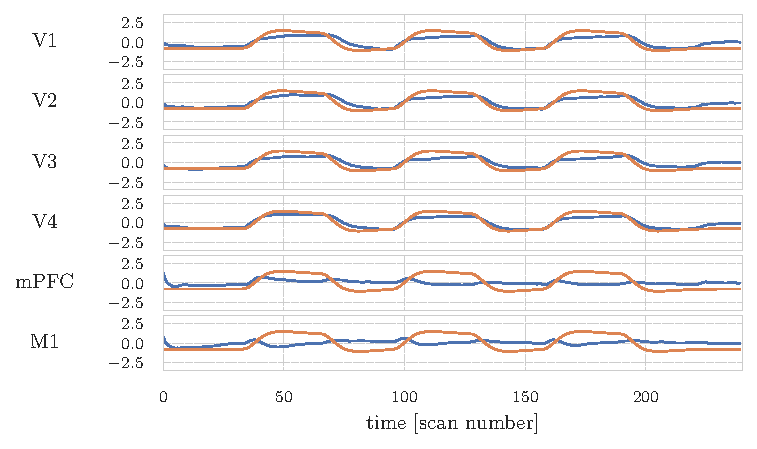
\includegraphics[width=\textwidth]{fig/rockland/CHECKERBOARD645/node_timeseries/mean_over_subjects}
  \caption{
    Rockland data normalized BOLD time series averaged over all 286 subjects.
    External visual stimulus convolved with HRF is shown for reference.
    As expected, correspondence to the external stimulus decreases as we move up and away from the visual processing hierarchy.
}\label{fig:rockland-time-series-mean-over-subjects}
\end{figure}


Initially, we aim to extract a well-understood phenomenon, related to the hierarchy in the visual cortex.
Based on the hierarchical nature of the visual cortex, we expect \gls{v1} to correlate most strongly with V2, followed by V3 and V4.
But what about \gls{mpfc} and \gls{m1}?
In fact, we quickly run into a recurring issue in the field: circular analysis~\parencite{Kerr1998, Kriegeskorte2009, Kriegeskorte2010, Poldrack2012, Poldrack2017}.
This motivates other ways of defining this benchmark.

%%
\subsubsection{External stimulus prediction}
%%


\begin{figure}[t]
  \centering
  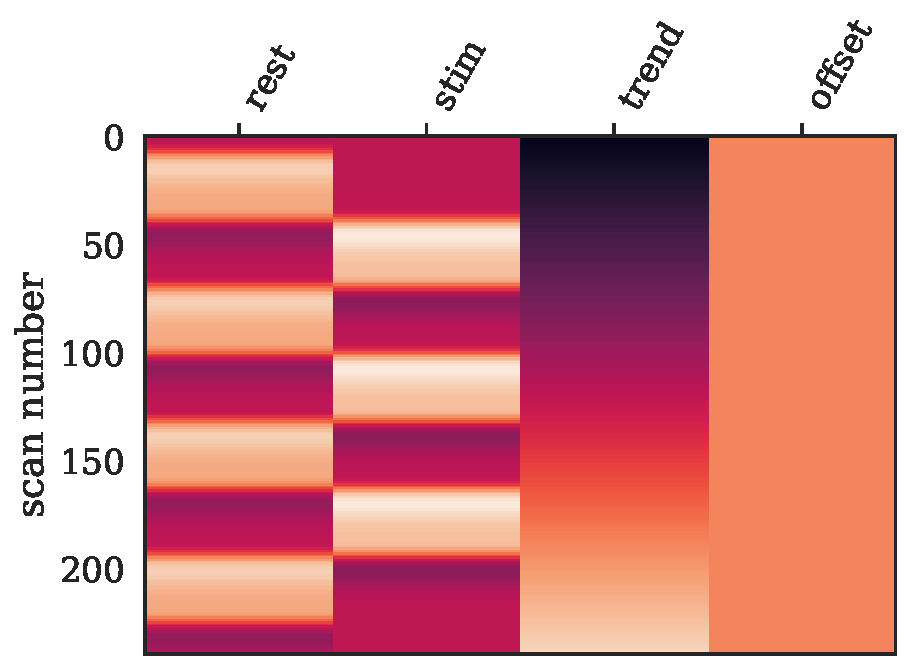
\includegraphics[width=0.6\textwidth]{fig/rockland/CHECKERBOARD645/prediction_benchmark/design_matrix_nilearn}
  \caption{
    Rockland benchmark design matrix $\mathbf{X}$ used for predicting external stimulus.
    The matrix is used by a GLM to determine how well the stimulus can be reconstructed from TVFC estimates.
  }\label{fig:rockland-design-matrix}
\end{figure}


The prediction task is framed as predicting the presence of the external visual stimulus.
We use a well-established technique in the domain of \gls{tb-fmri} based on the \gls{glm} and its \textbf{design matrix}.
The \gls{glm} is defined as
\begin{equation}
  \mathbf{Y} = \mathbf{X} \mathbf{\beta} + \mathbf{E},
\end{equation}
where $\mathbf{Y} \in \mathbb{R}^{G \times N}$ is the estimated \gls{tvfc} for a given method for all $G = 5$ edges of interest (i.e.~\gls{v1} connectivity with the other five \glspl{roi}),\footnote{This replaces the voxels by $N$ matrix used in typical \gls{fmri} studies~\parencite{Friston1995}.} $\mathbf{X} \in \mathbb{R}^{R \times N}$ is the design matrix with $R$ regressors (shown in \cref{fig:rockland-design-matrix}) weighted by $\beta \in \mathbb{R}^{R \times G}$, and $\mathbf{E} \in \mathbb{R}^{G \times N}$ are the error terms.
%
The regressors in $\mathbf{X}$ are hypothesized contributors to the experiment.
They can be divided into `experimental' regressors (those of interest) and `nuisance' regressors (those we expect to affect the measurements but are not of interest, such as motion parameters or physiological signals as heart rate).
Our experimental regressors are the boxcar (block design) model of the visual stimulus, convolved with the \gls{hrf}~\parencite{Glover1999}.
Our nuisance regressors are first-order polynomials.
The polynomial (drift) order was determined as \gls{tr} multiplied by~$\frac{N}{150}$~\parencite[see][for rationale]{Worsley2002}.
Effectively this reduces to allowing the model to \emph{detrend} the observed \gls{tvfc} estimates (this includes a constant value as well to remove the \emph{offset}).
Adding these can be considered similar to actively detrending the \gls{tvfc} estimates (e.g.~using bandpass filtering).
However, adding them to the design matrix allows the model to learn the relevance automatically.
This matrix is generated and plotted using the open-source Python library \texttt{Nilearn}~\parencite[][version~0.9.2]{Abraham2014}, which in turn is built upon \texttt{scikit-learn}~\parencite[][version~1.2.1]{Pedregosa2011} and \texttt{SciPy}~\parencite[][version~1.10.0]{SciPy2020}.
We infer $\mathbf{\beta}$ from the observations using \gls{ols} to minimize the error terms~$\mathbf{E}$~\parencite{Worsley1995}.
These $\beta$ parameters can then be used to determine which \gls{tvfc} estimates have captured the presence of the external visual stimulus best.
Entries in this regressor matrix indicate relative contributions of regressors in predicting $\mathbf{Y}$.

%%
\subsubsection{Implementational details}
%%

Only the \gls{vwp} model is trained here, as $N$ is reasonably small.

\clearpage
\section{Results}\label{sec:benchmarking-results}
%%%%%

Here we discuss the results of all benchmarking efforts.

%%
\subsection{Simulations}\label{sec:simulations-results}
%%

%%
\subsubsection{Data-driven hyperparameter optimization}
%%

First, we verify that the cross-validation of \gls{sw} window lengths (as described in \cref{sec:cross-validated-sw}) leads to improved covariance estimation.
\Cref{fig:sim-optimal-window-lengths} shows the learned optimal window lengths for each of the synthetic covariance structures.
As expected, the more \emph{static} the covariance structure is (e.g.~null and constant), the \emph{longer} the learned optimal window length $\hat{w}$ will be.
The faster the covariance structure changes over time, the smaller the optimal window length becomes.


\begin{figure}[ht]
  \centering
  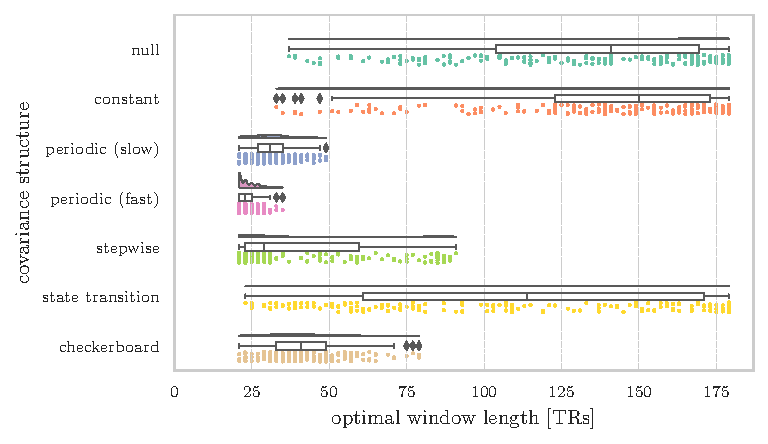
\includegraphics[width=\textwidth]{fig/sim/d2/N0400_T0200/no_noise/SW_cross_validated_optimal_window_lengths}
  \caption{
    Simulations benchmark optimal cross-validated window lengths learned from bivariate ($D = 2$) noiseless data for $N = 400$.
    Each dot represents one of $T = 200$ trials.
    Faster changing covariance structures result in shorter learned window lengths.
  }\label{fig:sim-optimal-window-lengths}
\end{figure}


Similarly, we can look at the learned kernel lengthscales $l$ from the trained \gls{wp} model, as shown in \cref{fig:sim-learned-kernel-lengthscales}.
These are consistent with the \gls{sw-cv} approach.
The more static the covariance structure, the larger the learned kernel lengthscales will be.
The faster the covariance structure changes over time, the smaller the learned kernel lengthscales becomes.
Interestingly, the constant case yields larger kernel lengthscales.
We attribute this mostly to the fact that the prior of the \gls{wp} assumes uncorrelated time series.
Furthermore, the large values learned for the state transition covariance structure indicate that the models were not able to learn this structure.
%
From this we infer that these two model parameters ($l$ and $\hat{w}$) may capture similar aspects of the covariance structure.


\begin{figure}[t]
  \centering
  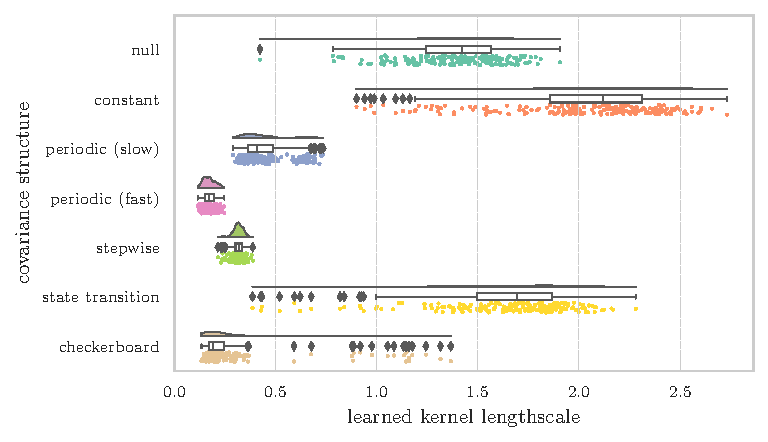
\includegraphics[width=\textwidth]{fig/sim/d2/N0400_T0200/no_noise/SVWP_kernel_lengthscales}
  \caption{
    Simulations benchmark SVWP kernel lengthscales $l$ learned from bivariate ($D = 2$) noiseless data for $N = 400$.
    Each dot represents one of $T = 200$ trials.
    Faster changing covariance structures result in shorter learned kernel lengthscales.
  }\label{fig:sim-learned-kernel-lengthscales}
\end{figure}


One key difference between the optimal window lengths and learned kernel lengthscales is that the latter are more distinct.
For example, given the lengthscales it is possible to perfectly distinguish between the slow and fast periodic covariance structures.
This is not the case for the window lengths, where there is still an overlap between these.

Another important observation is that even for the null and constant cases, our current implementation of \gls{sw-cv} still finds short optimal window lengths in some (rare) cases.
The same can be said for the \gls{wp} kernel lengthscales, although to a lesser degree.
In \cref{subsec:higher-dimensions} we touched upon running our models in pairwise fashion, which would increase the number of window length searches from 1 to $\frac{D (D - 1)}{2}$.
As such we would expect some edges to report false positives.
Perhaps the temporal character of some edges is truly different from others (requiring a different window length or different kernel lengthscale), but this warrants caution.

%%
\subsubsection{Bivariate case}
%%

We start with a qualitative visual inspection of bivariate \gls{tvfc} estimates.
Single trial examples for each method on the simulated data with $N = 400$ for all covariance structures are shown in \cref{fig:sim-results-tvfc-estimates-example}.
Both noiseless (\cref{fig:sim-results-bivariate-no-noise-all-covariance-structures-tvfc-predictions}) and the hybrid case with added \gls{hcp} \gls{rs-fmri} noise with an \gls{snr} of 2 (\cref{fig:sim-results-bivariate-HCP-noise-all-covariance-structures-tvfc-predictions}) are shown.
Results for other values of $N$ and noise configurations can be found in \cref{ch:appendix-d2-impact-of-noise}.


\begin{figure}[t]
  \centering
  \subcaptionbox{Without noise\label{fig:sim-results-bivariate-no-noise-all-covariance-structures-tvfc-predictions}}{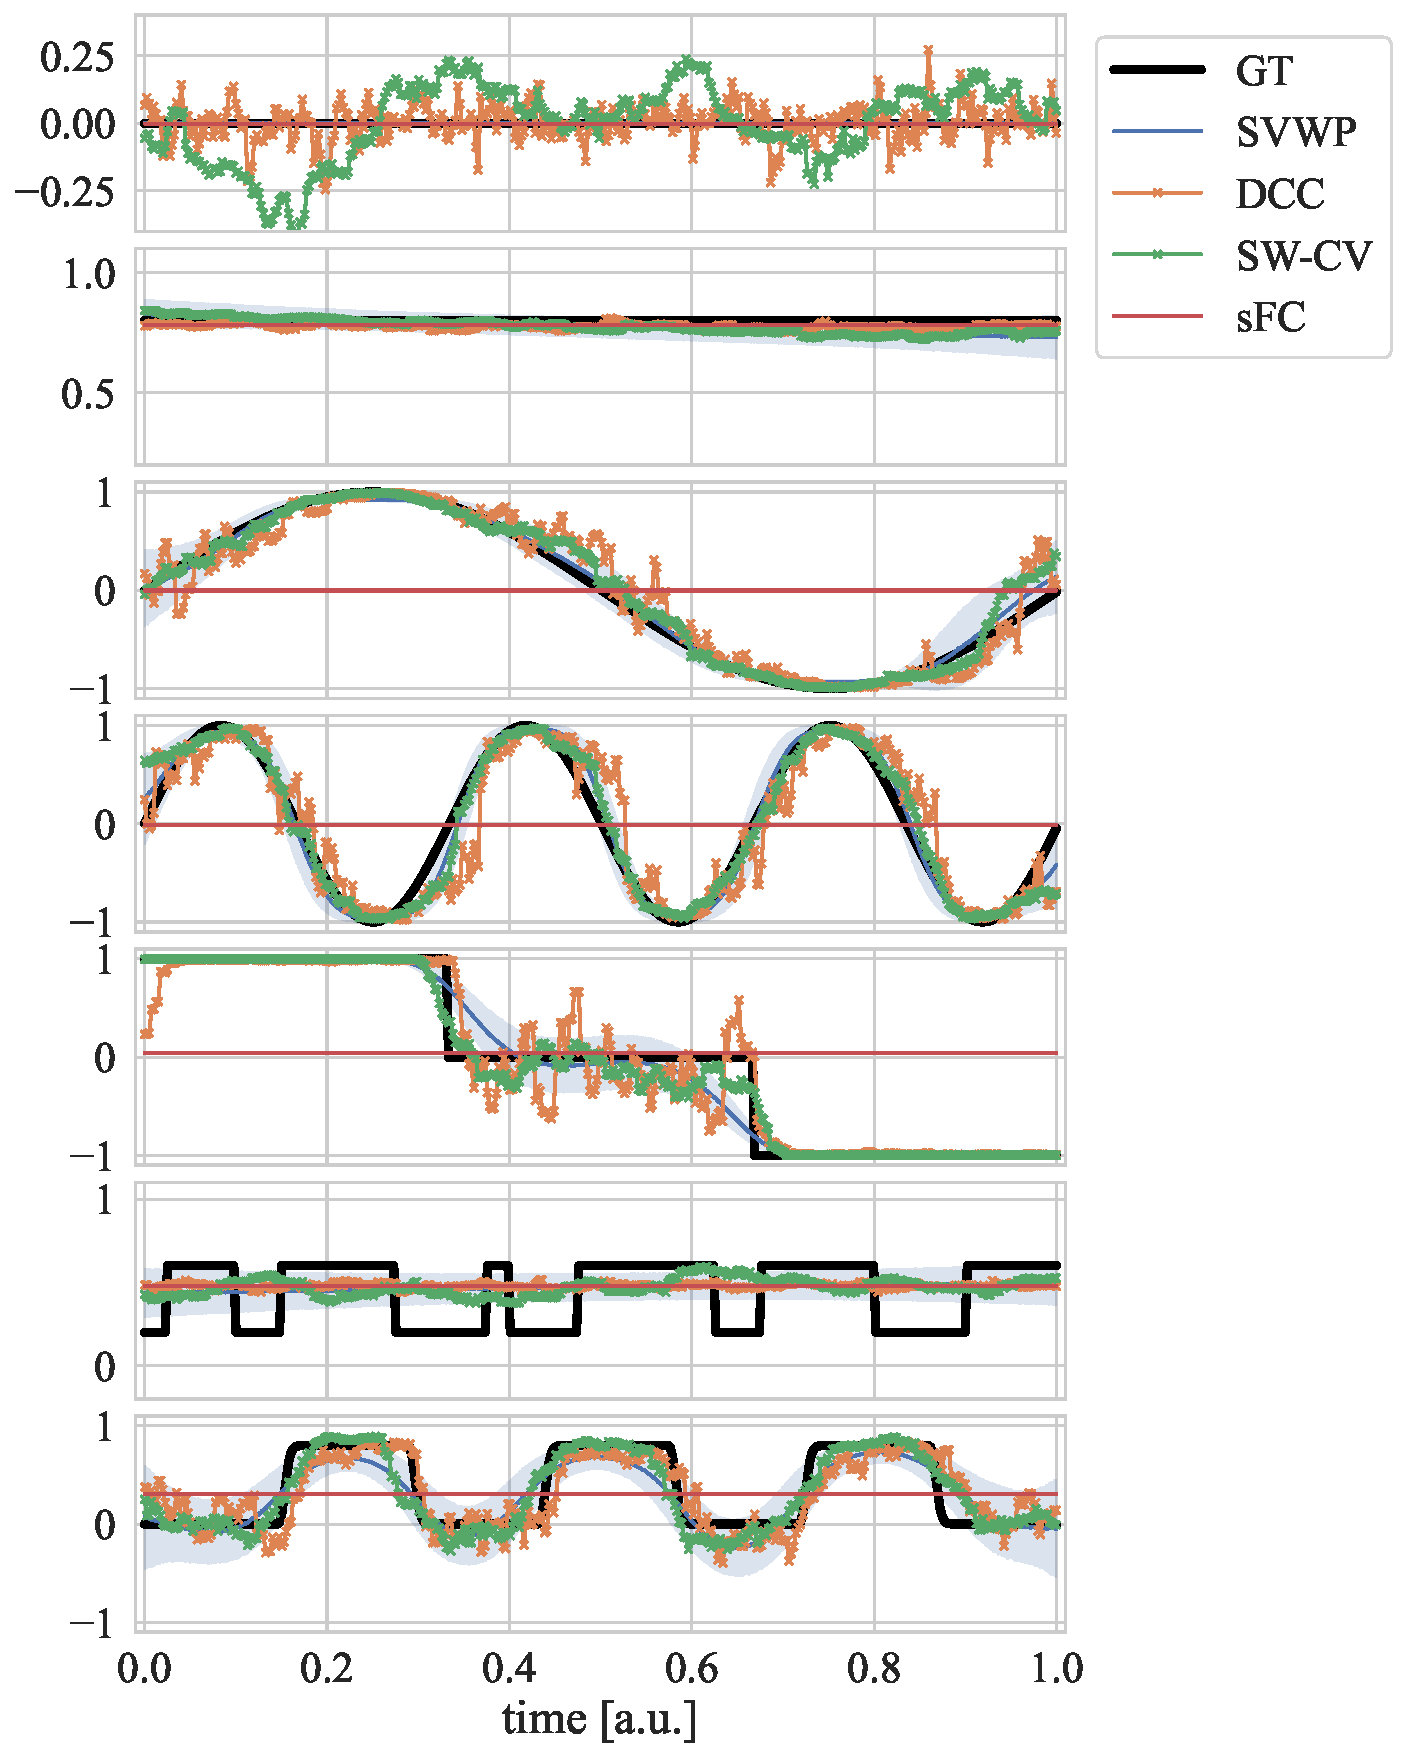
\includegraphics[width=0.48\textwidth]{fig/sim/d2/N0400_T0200/no_noise/all_covs_types_correlations}}
  \subcaptionbox{With rs-fMRI noise (hybrid)\label{fig:sim-results-bivariate-HCP-noise-all-covariance-structures-tvfc-predictions}}{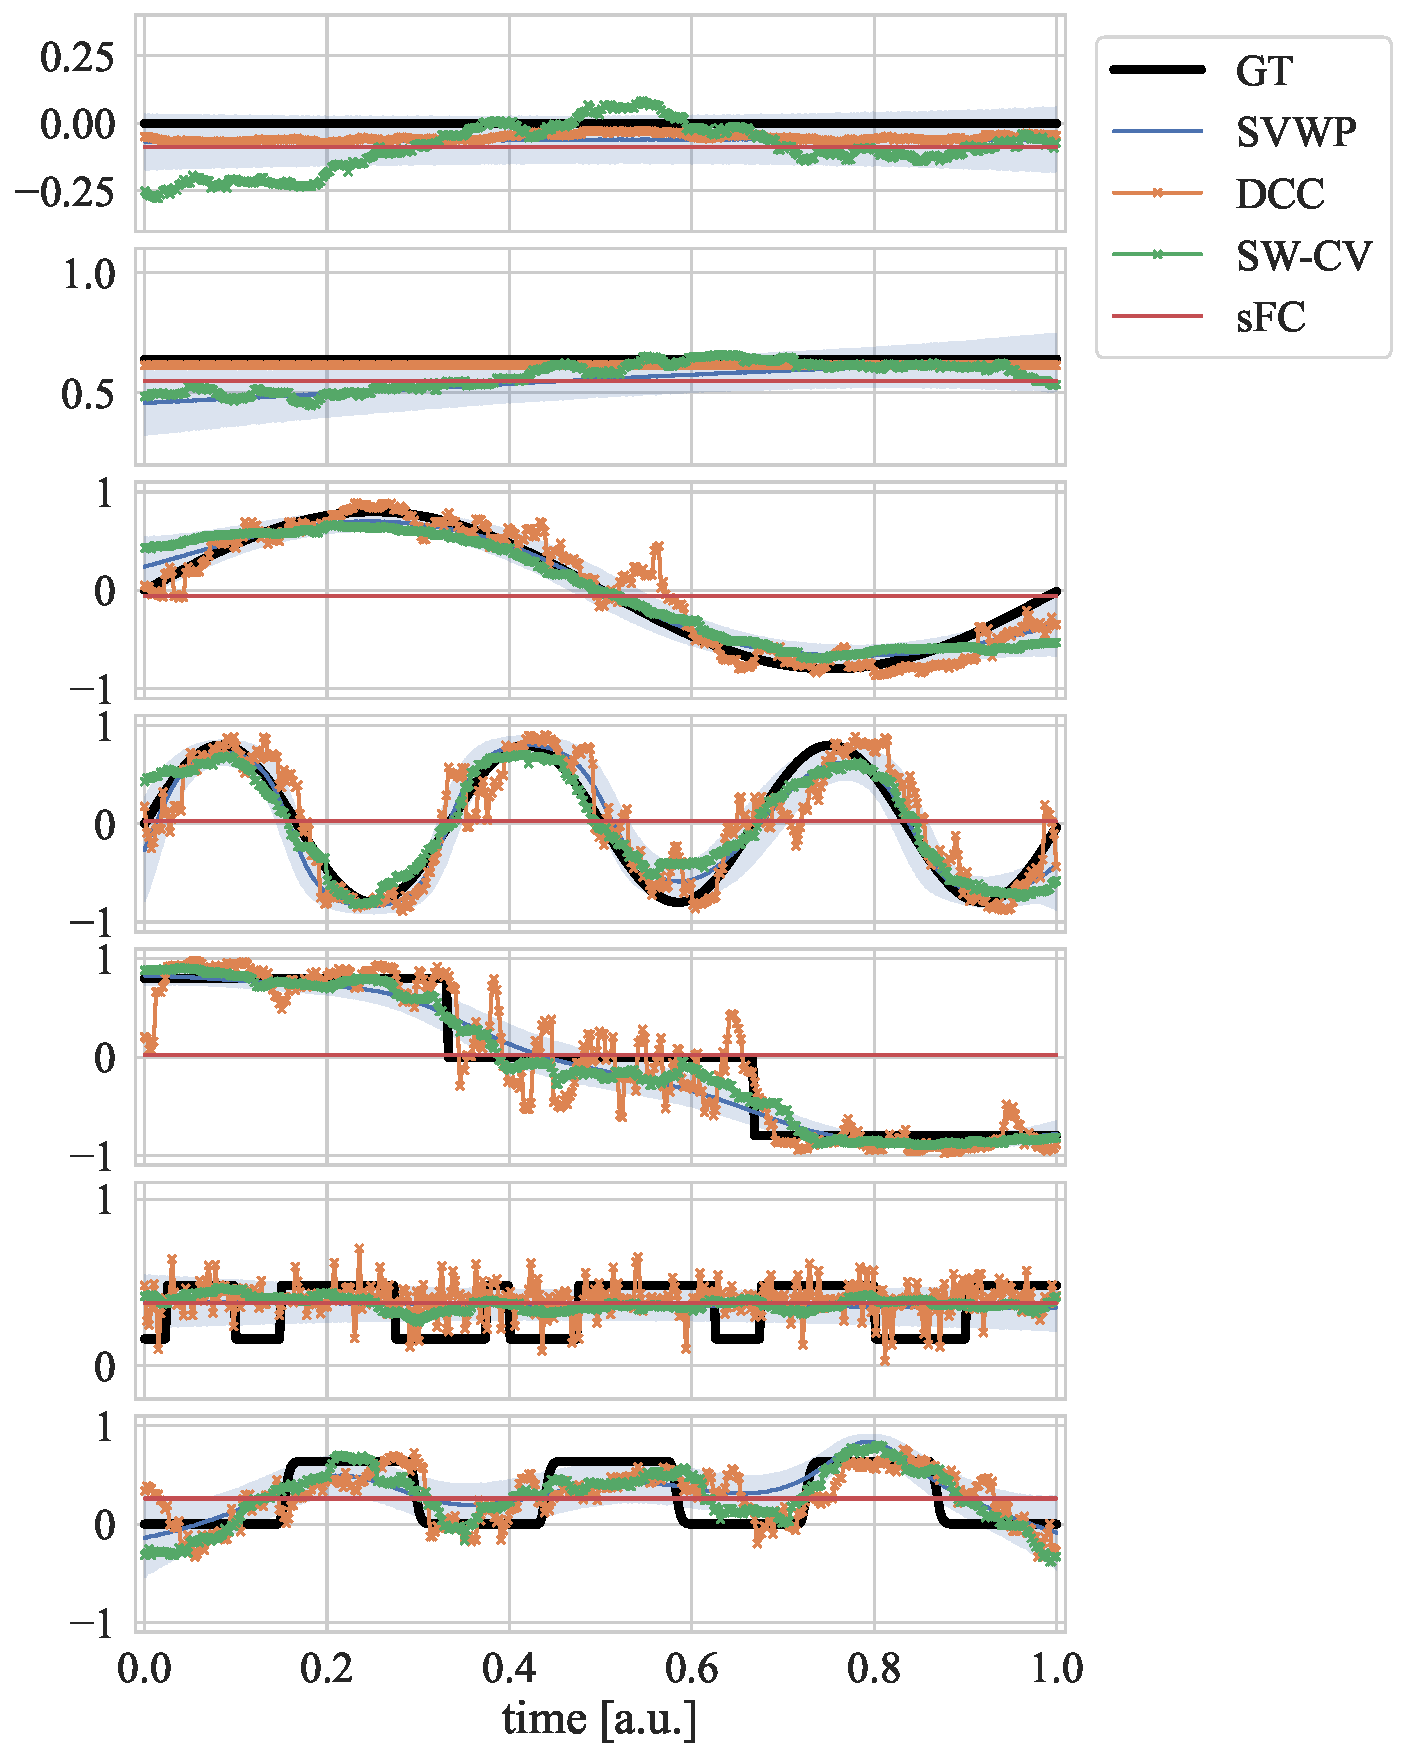
\includegraphics[width=0.48\textwidth]{fig/sim/d2/N0400_T0200/HCP_noise_snr_2/all_covs_types_correlations}}
  \caption{
    Simulations benchmark single trial TVFC estimates for all covariance structures, for bivariate data ($D = 2$) for $N = 400$.
    Ground truth (GT) is included for reference.
    Estimation methods have distinct failure modes.
  }\label{fig:sim-results-tvfc-estimates-example}
\end{figure}


Failure modes of the different \gls{tvfc} estimation methods are clearly visible.

For the two static covariance structures (null and constant), even the cross-validated \gls{sw} method detects spurious time-varying structure.
This \gls{sw} failure mode has been long known in the field~\parencite{Lindquist2014, Hindriks2016}.
The \gls{dcc} and \gls{svwp} models remain close to the ground truth.

For the two periodic covariance structures, the \gls{sfc} estimate is not sensitive to this structure, unlike for the null and constant covariance structure data.
\gls{sw-cv} performs well and picks the correct window length in both cases.
The \gls{mgarch} model captures the structure as well, although spurious sudden large jumps are seen.
We see that the \gls{svwp} can model smooth changes in covariance structure well (indeed, this is perhaps where it excels).
From visual inspection it seems to return the best fit.
It is worth pointing out as well that the \gls{sw-cv} estimates at all time steps fall within the uncertainty bounds of the \gls{svwp} estimates.

For the stepwise data, we can see that the \gls{svwp} estimates are too smooth and perform poorly during sudden changes in covariance structure.
This is an expected failure mode, as this model expects slowly changing covariance.
Moreover, the `static' part of the time series requires a longer lengthscales, whereas the sudden jumps would require a shorter lengthscales.
The \gls{sw-cv} estimates suffer from a similar problem, where it is not clear what window length would be optimal here.
The \gls{dcc} method deals well with the change points but shows a lot of jumps in the middle of the time series.
As they are autoregressive models, they do not work well for the beginning of the time series either.
This could be mitigated, however, by removing the first several volumes from the analysis, which is common practice in \gls{fmri} studies (usually no more than six).
These first volumes are often considered unreliable because the participant and scanner are `settling in' during these.
Crucially, these plots show that estimates are vastly different in nature, and without knowing our eventual use case it is hard to say which estimates are superior here.

All methods fail to pick up the state transition covariance structure, although in different ways.
The \gls{svwp} predicts like it is static (with a large uncertainty bound), and \gls{dcc} and \gls{sw} estimates jump around a little, sometimes seemingly capturing some of the structure.
Interestingly, these estimates look like the ones made for the static covariance cases.
So, if we would have not known any ground truth, it would have been unclear if the underlying process was static or showed state transitions as simulated here.
The fact that none of the methods can pick up on this structure also raises concern about whether we need completely different approaches if such underlying structure is to be expected in real data.
How subtle do we expect changes in \gls{tvfc} with shifting cognitive state?
How many of such changes do we expect per minute?
We will return to this issue in \cref{subsec:sudden-changes}.

Finally, for the checkerboard data, all time-varying methods pick up generally on the covariance structure.
Method characters are different, however, with the \gls{svwp} estimates again being overly smooth and the other methods estimating many discontinuities.
There are several trials where the \gls{svwp} fails to learn the structure for lower values of $N$.


\begin{figure}[ht]
  \centering
  \subcaptionbox{Bivariate case ($D = 2$)\label{fig:sim-results-d2-HCP-noise-all-correlation-RMSE}}{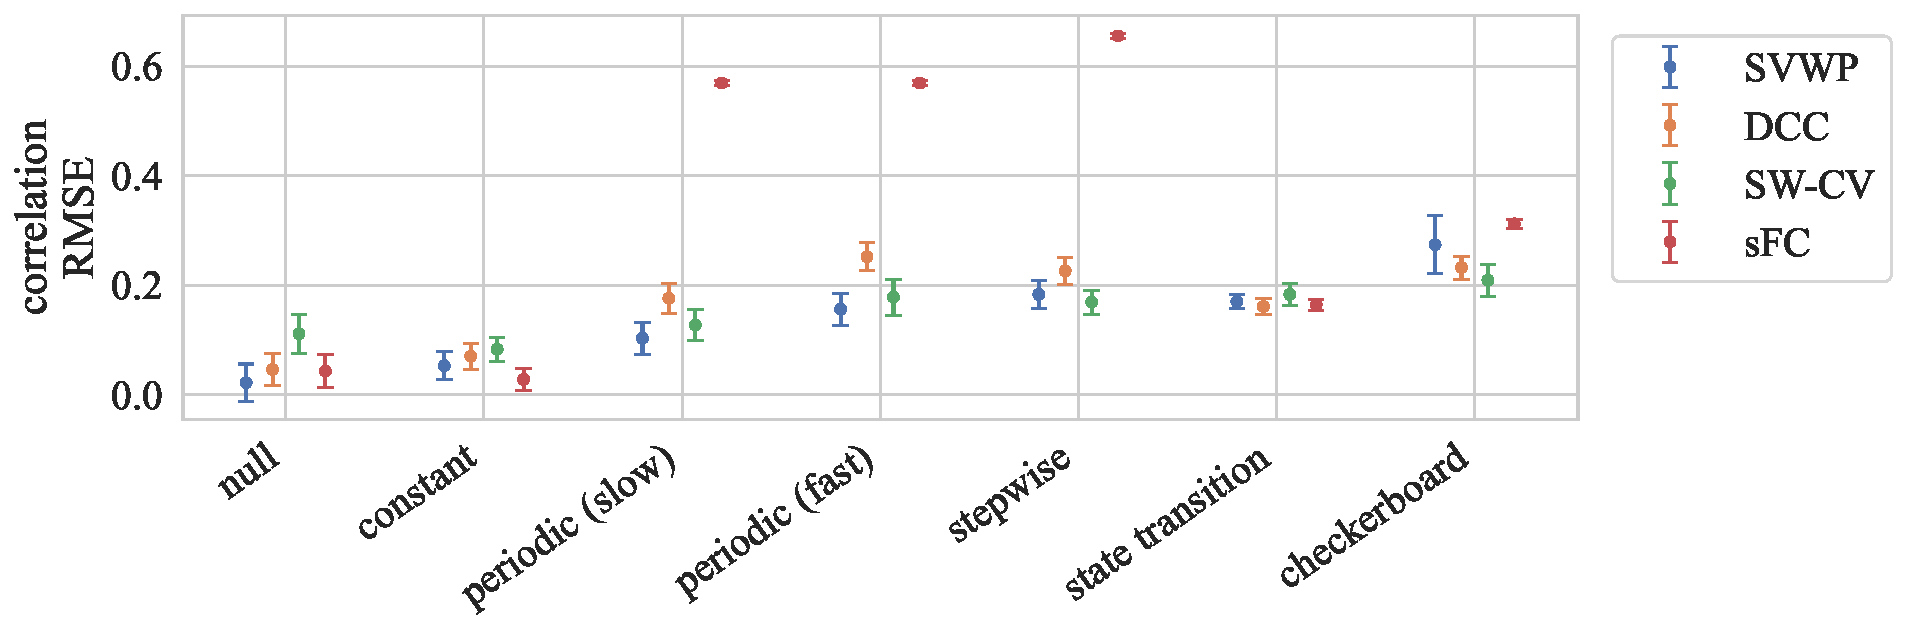
\includegraphics[width=0.84\textwidth]{fig/sim/d2/N0400_T0200/HCP_noise_snr_2/correlation_RMSE}}
  \subcaptionbox{Trivariate dense case ($D = 3$)\label{fig:sim-results-d3d-HCP-noise-all-correlation-matrix-RMSE}}{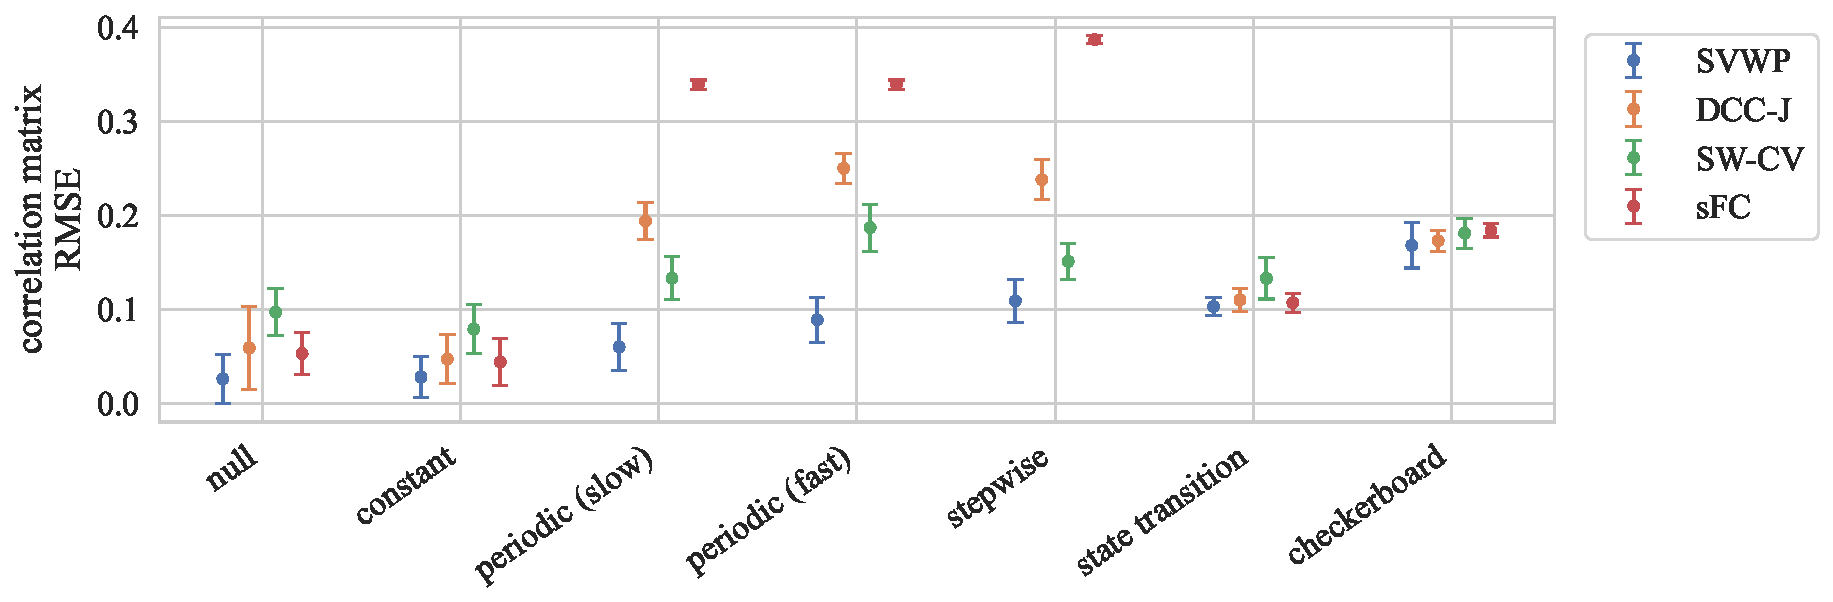
\includegraphics[width=0.84\textwidth]{fig/sim/d3d/N0200_T0200/HCP_noise_snr_2/correlation_matrix_RMSE}}
  \subcaptionbox{Trivariate sparse case ($D = 3$)\label{fig:sim-results-d3s-HCP-noise-all-correlation-matrix-RMSE}}{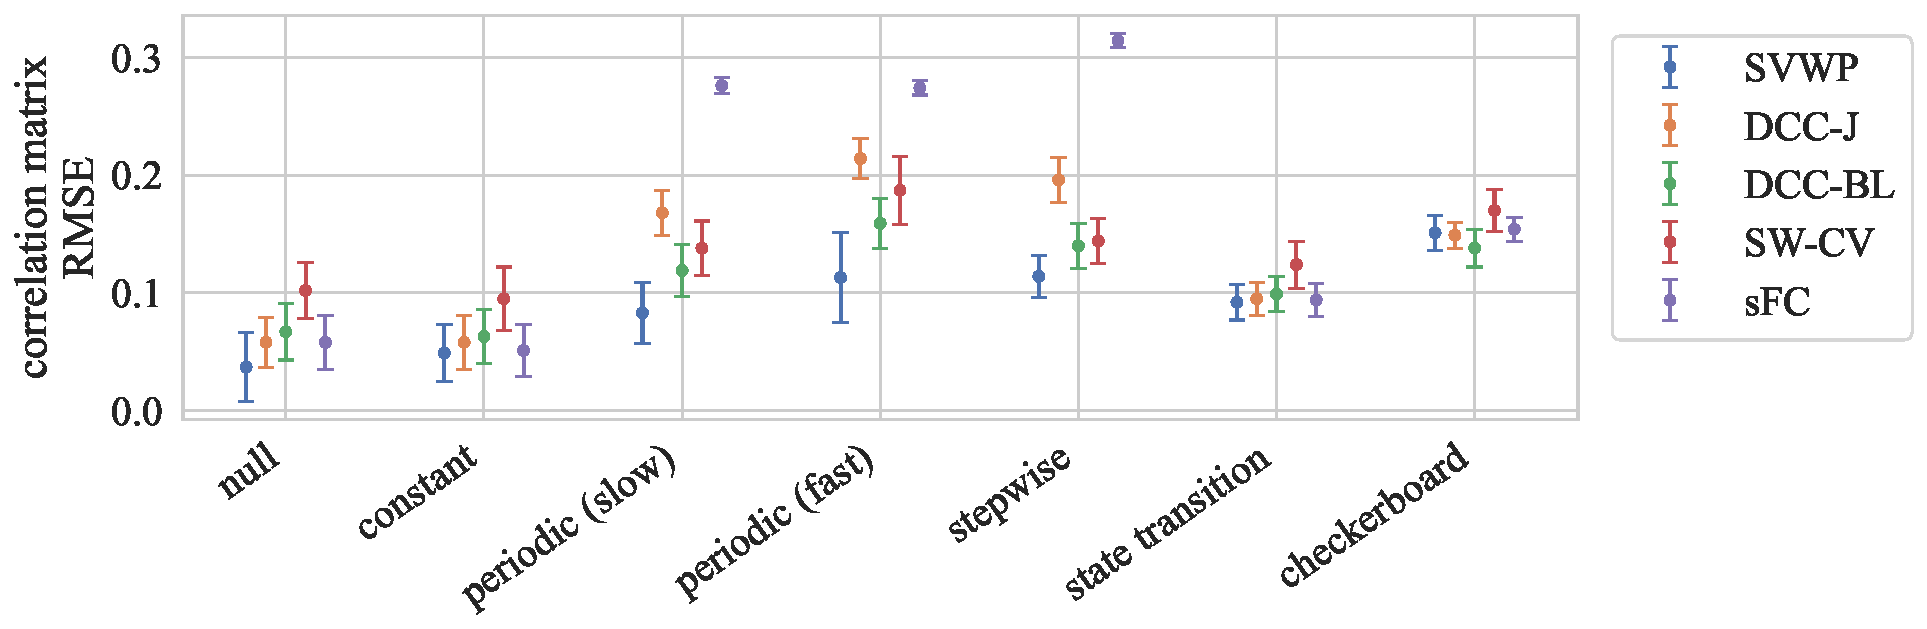
\includegraphics[width=0.84\textwidth]{fig/sim/d3s/N0200_T0200/HCP_noise_snr_2/correlation_matrix_RMSE}}
  \caption{
    Simulations benchmark RMSE between model TVFC estimates and ground truth on all bivariate and trivariate covariance structures with added rs-fMRI noise (SNR of 2) for $N = 400$.
    Means and standard deviations are shown across $T = 200$ trials.
  }\label{fig:sim-results-HCP-noise-all}
\end{figure}


Although the visual inspection of this single trial gives us intuition for model performance and failure modes, to compare methods robustly we need to \emph{quantify} model performance.
The computed \gls{rmse} between estimated and ground truth correlation terms (i.e.~the off-diagonal term) is shown in \cref{fig:sim-results-d2-HCP-noise-all-correlation-RMSE}.
The results are shown for the hybrid case, as a noisier setup is considered more realistic.
%
These quantitative results generally confirm our intuition from the visual inspection.
The \gls{svwp} and \gls{dcc} models perform like a single window approach for the null and constant cases, with the \gls{sw-cv} performing slightly worse.
The \gls{svwp} is better at modeling the smooth periodic covariance structures, whereas the \gls{dcc} model picks up relatively better on the sudden changes of the stepwise covariance structure.
The \gls{sw-cv} performs well overall on the dynamic covariance structures.
The \gls{sfc} estimate, as expected, performs well on static covariance structures, and fails on the time-varying structure.
Interestingly, the \gls{wp} even \emph{outperforms} \gls{sfc} on null covariance, which is likely due to its prior (mean function) expecting zero correlation.
%
However, none of the methods can significantly outperform the \gls{sfc} estimate on the state transition covariance structure.
This result can be considered a quantitative confirmation of our hypothesis from looking at the estimates.
This structure may be too hard to learn by the methods considered.
This point was made by \textcite{Lindquist2014} too, who claimed that \gls{dcc} cannot model abrupt changes (change points) well.
Results for $N = 120$, $N = 200$, and $N = 1200$ show similar relative performance (see \cref{appendix:sim-more-quantitative-results}).
%
Model estimates may look different despite having similar reconstruction errors, as is the case for the stepwise covariance structure, for example.
This highlights the limit of using such a performance metric alone.
%
Lastly, based on these results we posit that a method's outperformance of the \gls{sfc} can be considered an indication of how time-varying the covariance structure is.
If a dynamic method's performance is similar to that of \gls{sfc}, either there is no or little dynamic structure present, or the method has failed to pick up on it (e.g.~state transition).

%%
\subsubsection{Trivariate cases}
%%

Recall that for the trivariate ($D = 3$) case we train \gls{dcc} both in a pairwise and joint manner.
Some illustrative \gls{tvfc} estimates are shown in \cref{ch:appendix-d3-tvfc-estimates}.
We make similar observations as for the bivariate case.
For the null case (\cref{fig:results-d3-no-noise-null-covariance}) we see that the \gls{sw-cv} estimates still return time-varying structure.
Interestingly, the pairwise \gls{dcc} here performs worse than the jointly trained one.
This may be due to this \gls{dcc} still returning spurious structure when given just two time series (as we have seen in the bivariate case).
For the dense trivariate case (\cref{fig:results-d3s-no-noise-periodic-3-covariance}) we see \gls{tvfc} estimates similar to the ones for the bivariate case.
However, the sparse case (\cref{fig:results-d3s-no-noise-stepwise-covariance}) reveals that it may be a good idea to train \gls{dcc} in a pairwise manner.
The jointly trained \gls{dcc} model performs much worse here.

Quantitative results for the dense and sparse trivariate cases with added \gls{hcp} \gls{rs-fmri} noise are shown in \cref{fig:sim-results-d3d-HCP-noise-all-correlation-matrix-RMSE} and \cref{fig:sim-results-d3s-HCP-noise-all-correlation-matrix-RMSE}.
We generally see the same trends in these results as for the bivariate case.
The \gls{svwp} does relatively well on the sparse covariance structures, and the jointly trained \gls{dcc} does relatively poorly here.

%%
\subsubsection{Toward higher dimensions}
%%

Real applications would typically have more than $D = 3$ nodes (e.g. 15, 6, 9, and 3 for the subsequent respective studies in this thesis).
The sparse implementation can be scaled to any number of dimensions.
Running this on higher dimensions maintains the same trends as we saw for the bivariate and trivariate cases.
However, more complicated covariance structures in higher dimensions are left for future work.

%%
\subsubsection{Impact of noise analysis}\label{subsec:impact-of-noise-analysis}
%%

To understand the impact of noise on our results, the estimates for various noise levels are shown in \cref{ch:appendix-d2-impact-of-noise,ch:appendix-d3d-impact-of-noise}.
All methods gradually perform worse with lower \glspl{snr}.
We see most methods breaking down with the \gls{snr} of 1.
However, some methods break down before others.

%%
\subsubsection{Imputation benchmark}
%%

The imputation benchmark (\cref{subsec:imputation-benchmark}) is also run on all synthetic covariance structures.
We are mainly interested in comparing the performance on this benchmark to the reconstruction errors discussed before.
%
Let us look at two cardinal cases, both using bivariate, noiseless data.
For the null covariance case (\cref{fig:sim-imputation-study-d2-null}), we find all methods to perform similarly well on the imputation benchmark.
This was to be expected.
All models can model this appropriately, as witnessed in both the visual inspection and the quantified results.
\gls{sw-cv} performs slightly worse than the other methods, which again was to be expected as it also performed slightly worse on the other performance metrics.
However, for a non-static covariance structure such as the slowly oscillating periodic one, we find the \gls{sfc} estimates to perform much worse on the imputation benchmark than the other methods (see \cref{fig:sim-imputation-study-d2-periodic-1}).
We find the \gls{svwp} to perform best on this benchmark.
Thus, we obtained results \emph{without} using a ground truth, that correspond well to the performance metrics computed \emph{with} knowledge of a ground truth.
This is exciting, as this imputation benchmark can be run on any (real) data set.


\begin{figure}[t]
  \centering
  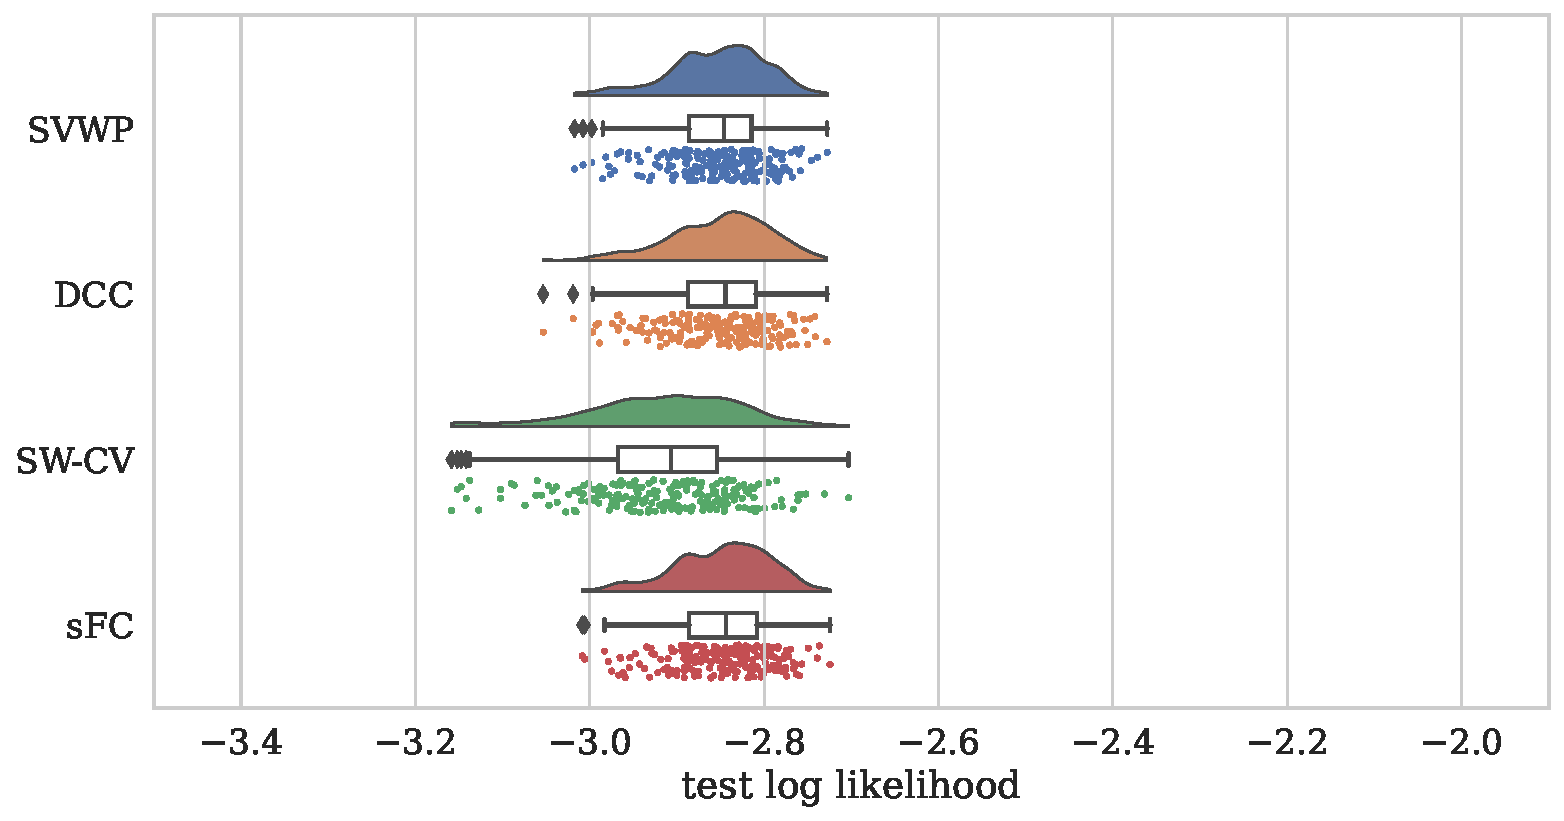
\includegraphics[width=\textwidth]{fig/sim/d2/N0400_T0200/imputation_study/LEOO_no_noise_test_log_likelihoods_raincloud_null}
  \caption{
    Simulations imputation benchmark - null covariance.
    Test log likelihoods for bivariate ($D = 2$) noiseless data for $N = 400$.
    Each dot represents one of $T = 200$ trials.
  }\label{fig:sim-imputation-study-d2-null}
\end{figure}


\begin{figure}[t]
  \centering
  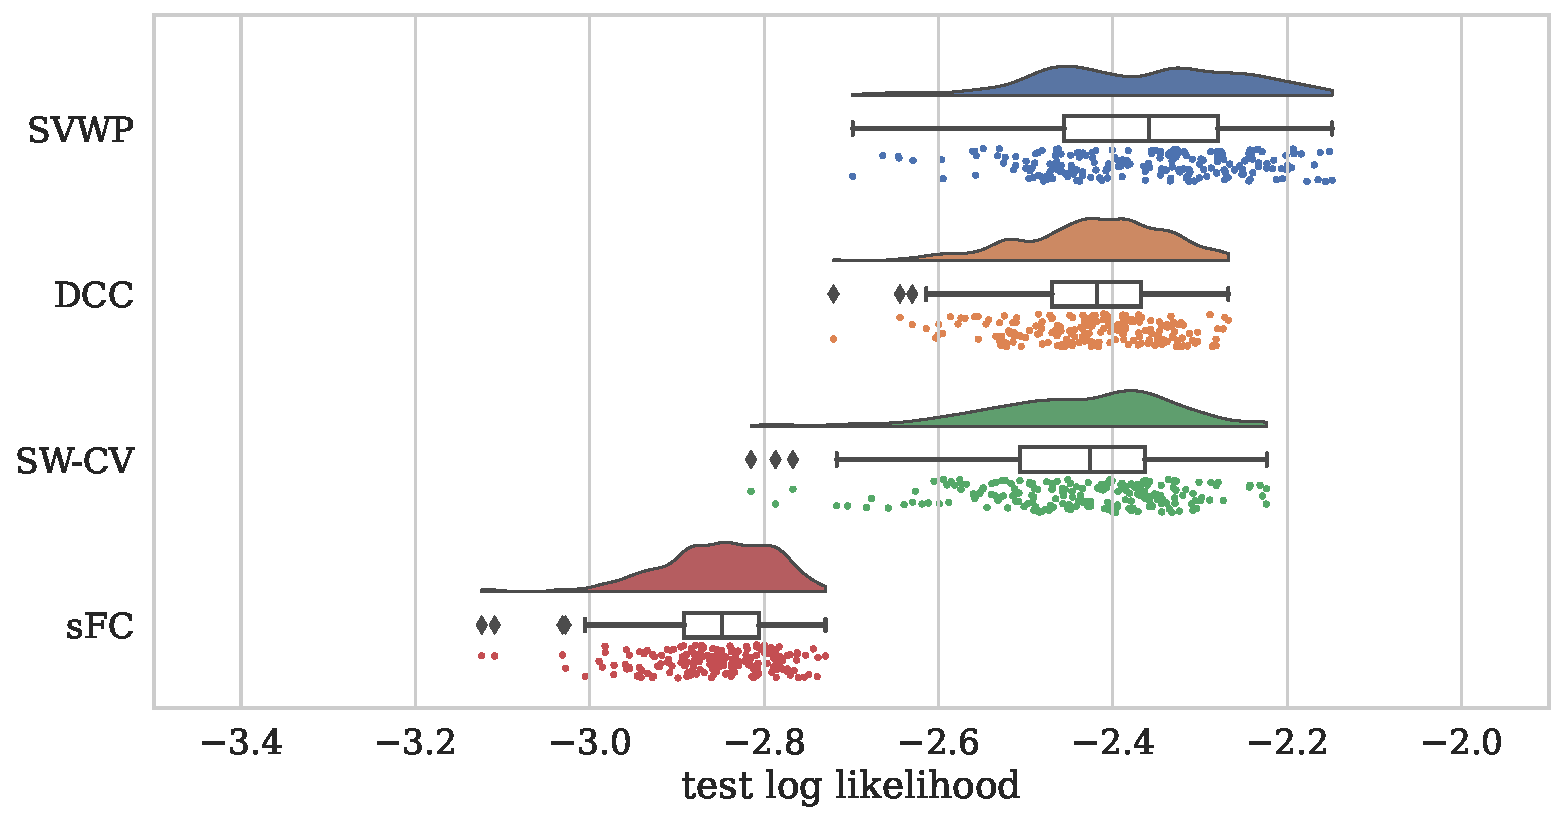
\includegraphics[width=\textwidth]{fig/sim/d2/N0400_T0200/imputation_study/LEOO_no_noise_test_log_likelihoods_raincloud_periodic_1}
  \caption{
    Simulations imputation benchmark - periodic (slow) covariance.
    Test log likelihoods for bivariate ($D = 2$) noiseless data for $N = 400$.
    Each dot represents one of $T = 200$ trials.
  }\label{fig:sim-imputation-study-d2-periodic-1}
\end{figure}


%%
\clearpage
\subsection{Resting-state fMRI}\label{subsec:hcp-results}
%%

Before diving into any quantitative results, we should again visually inspect the estimated \gls{tvfc} from different methods.
This time we study a real \gls{fmri} data set.
Estimates for several edges of a single scan of a single subject from the \gls{hcp} data set ($D = 15$) are shown in \cref{fig:hcp-model-estimates-example}.


\begin{figure}[ht]
  \centering
  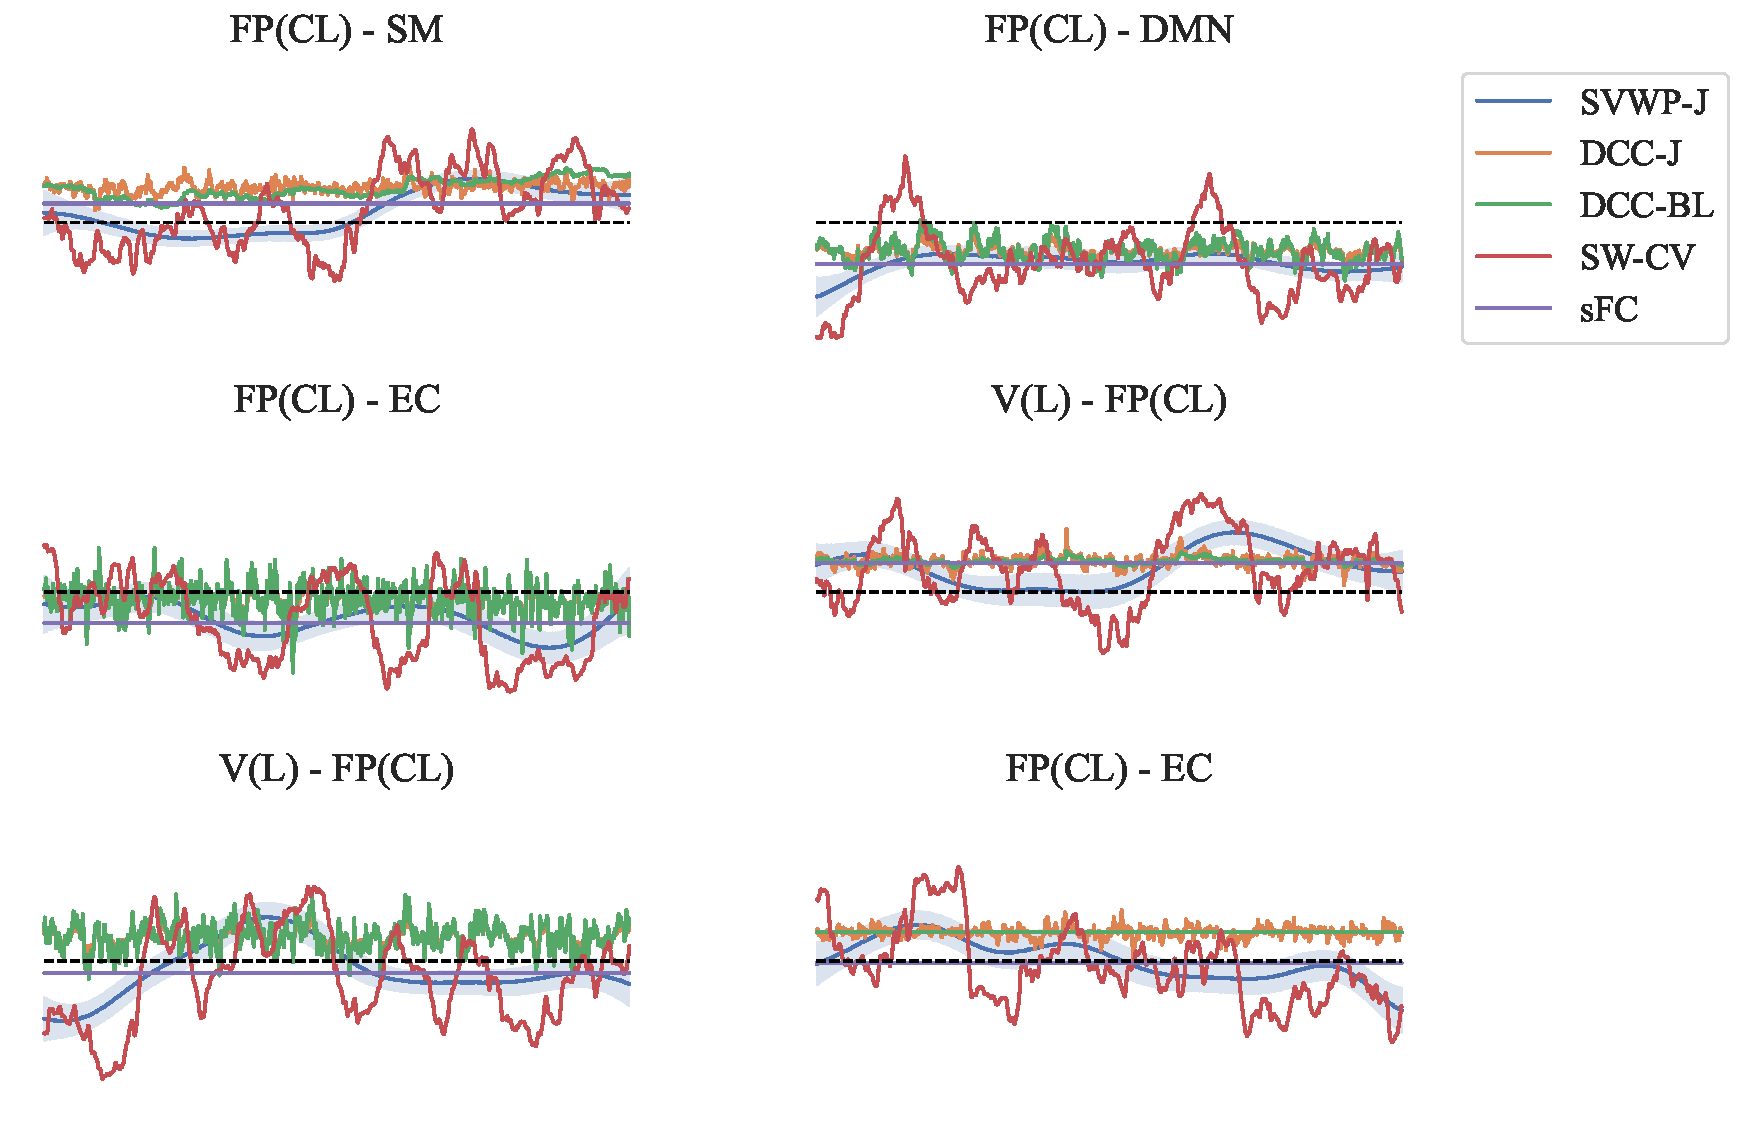
\includegraphics[width=\textwidth]{fig/hcp/d15/TVFC_predictions/scan_0/all/100206/correlation_estimates_random_edges}
  \caption{
    HCP benchmark TVFC estimates for random selection of edges (from $D = 15$ time series) for a single scan of a single HCP subject.
    The y-axis scales from~-1~to~1; the black dashed line indicates zero correlation.
    Method estimates vary radically.
}\label{fig:hcp-model-estimates-example}
\end{figure}


Several observations can be made from visual inspection.
%
First, there is a large variety in general correlation (connectivity strength) between the edges.
Albeit with fluctuations, some edges are consistently strongly correlated, whereas others are generally uncorrelated.
Some edges show dynamics, whereas others appear more static.
This was to be expected, as brain region interactions should be distinct from one another.
%
Secondly, perhaps worryingly, estimates vary radically among the methods considered.
The mean of \gls{tvfc} estimates across time for both the \gls{svwp} and \gls{sw} methods is consistent with the \gls{sfc} estimate, in contrast to the \gls{dcc} estimates.
We also see major differences between \gls{tvfc} estimates in terms of how fast \gls{tvfc} changes.
The \gls{sw} method estimates constantly and rapidly changing \gls{tvfc}, with large variance across time.
The \gls{svwp} method estimates time-varying but transiently changing \gls{tvfc}.
The \gls{dcc} method estimates rapidly changing \gls{tvfc}, but constricted to a small range (i.e.~low variance).
%
Lastly, we observe that the \gls{svwp} estimates look like a smooth version of the \gls{sw-cv} estimates.
This could mean that either the \gls{svwp} model cannot pick up on the fast-changing nature of \gls{tvfc}, or that the \gls{sw-cv} method picks up on spurious fluctuations (yet still captures the general trends).
Training \gls{dcc} in a joint or pairwise manner does not seem to make a significant difference here.
%
These insights have been qualitatively verified by inspecting other scans.


\begin{figure}[t]
  \centering
  \subcaptionbox{SVWP-J\label{fig:HCP-model-estimates-summary-measures-mean-SVWP}}{\includegraphics[width=0.30\textwidth]{fig/hcp/d15/TVFC_predictions_summaries/scan_0/all/correlation_TVFC_mean_SVWP_joint}}
  \subcaptionbox{DCC-J\label{fig:HCP-model-estimates-summary-measures-mean-DCC}}{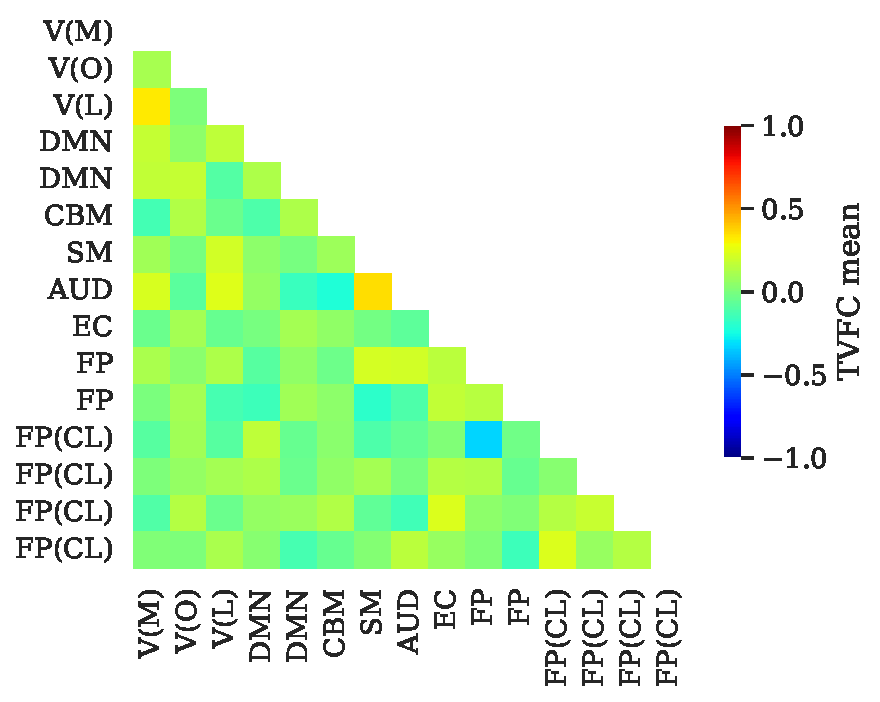
\includegraphics[width=0.30\textwidth]{fig/hcp/d15/TVFC_predictions_summaries/scan_0/all/correlation_TVFC_mean_DCC_joint}}
  \subcaptionbox{SW-CV\label{fig:HCP-model-estimates-summary-measures-mean-SW}}{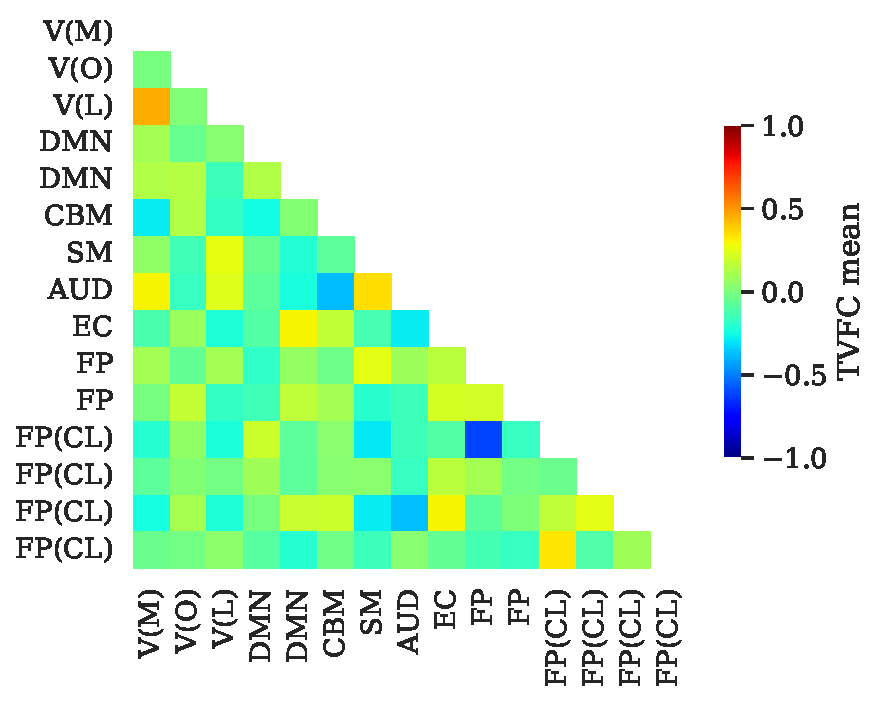
\includegraphics[width=0.30\textwidth]{fig/hcp/d15/TVFC_predictions_summaries/scan_0/all/correlation_TVFC_mean_SW_cross_validated}}
  \subcaptionbox{SVWP-J\label{fig:HCP-model-estimates-summary-measures-var-SVWP}}{\includegraphics[width=0.30\textwidth]{fig/hcp/d15/TVFC_predictions_summaries/scan_0/all/correlation_TVFC_variance_SVWP_joint}}
  \subcaptionbox{DCC-J\label{fig:HCP-model-estimates-summary-measures-var-DCC}}{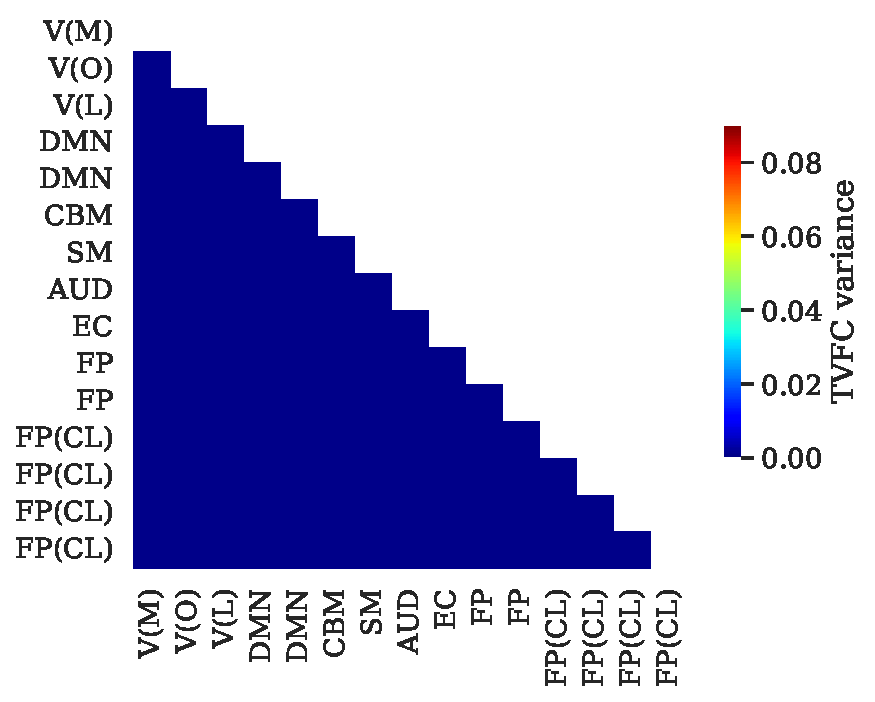
\includegraphics[width=0.30\textwidth]{fig/hcp/d15/TVFC_predictions_summaries/scan_0/all/correlation_TVFC_variance_DCC_joint}}
  \subcaptionbox{SW-CV\label{fig:HCP-model-estimates-summary-measures-var-SW}}{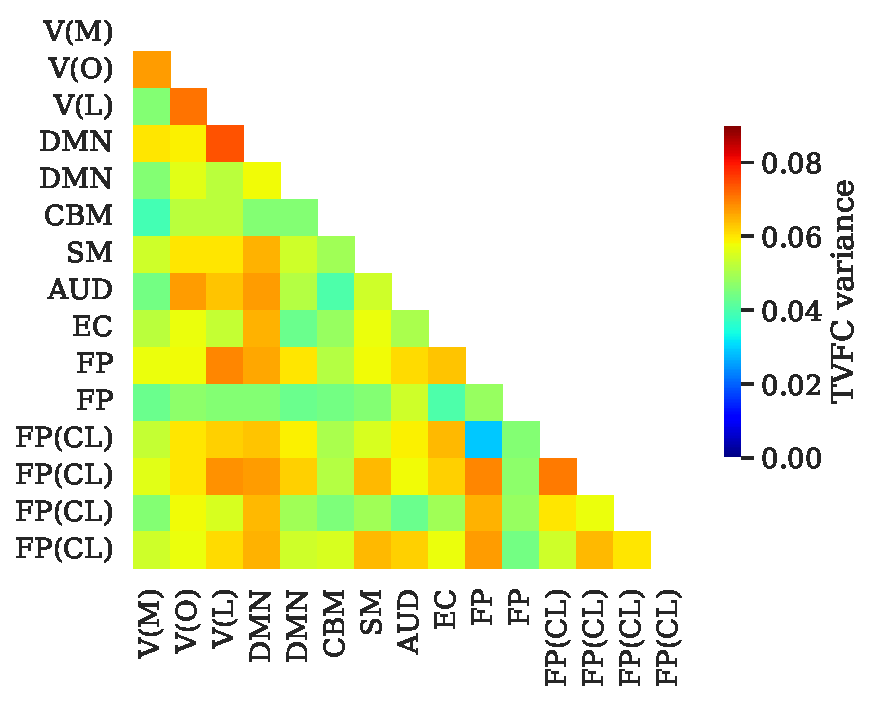
\includegraphics[width=0.30\textwidth]{fig/hcp/d15/TVFC_predictions_summaries/scan_0/all/correlation_TVFC_variance_SW_cross_validated}}
  \subcaptionbox{SVWP-J\label{fig:HCP-model-estimates-summary-measures-roc-SVWP}}{\includegraphics[width=0.30\textwidth]{fig/hcp/d15/TVFC_predictions_summaries/scan_0/all/correlation_TVFC_rate_of_change_SVWP_joint}}
  \subcaptionbox{DCC-J\label{fig:HCP-model-estimates-summary-measures-roc-DCC}}{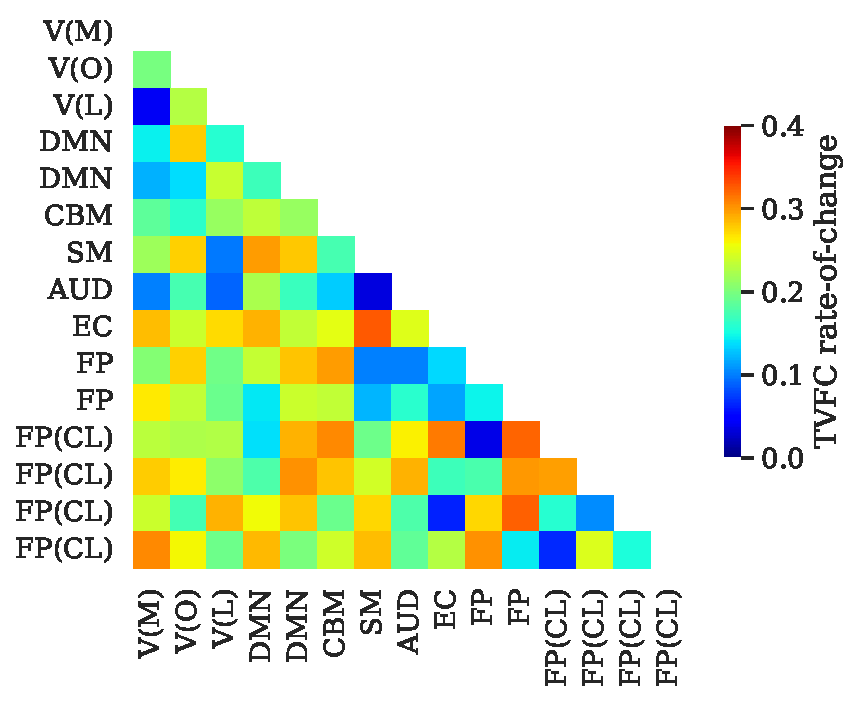
\includegraphics[width=0.30\textwidth]{fig/hcp/d15/TVFC_predictions_summaries/scan_0/all/correlation_TVFC_rate_of_change_DCC_joint}}
  \subcaptionbox{SW-CV\label{fig:HCP-model-estimates-summary-measures-roc-SW}}{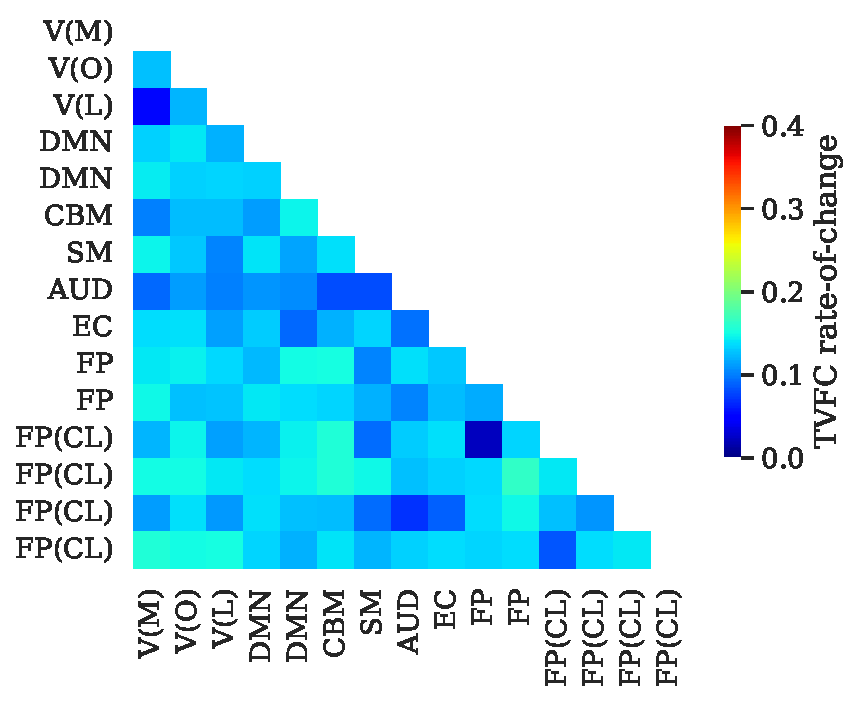
\includegraphics[width=0.30\textwidth]{fig/hcp/d15/TVFC_predictions_summaries/scan_0/all/correlation_TVFC_rate_of_change_SW_cross_validated}}
  \caption{
    HCP benchmark edgewise TVFC summary measures of first scan (1A) averaged over all subjects.
    TVFC mean (top), variance (middle), and rate-of-change (bottom row) are shown.
    For interpretation, ICA components are mapped to FNs.
    Visual (V): medial (M), occipital (O), lateral (L); Default Mode Network (DMN); Cerebellum (CBM); Sensorimotor (SM); Auditory (AUD); Executive Control (EC); Frontoparietal (FP) with Cognition-Language (CL) subset.
  }\label{fig:HCP-model-estimates-summary-measures}
\end{figure}


These distinct differences in dynamics can be captured by three \gls{tvfc} summary measures: mean, variance, and rate-of-change (see \cref{subsec:tvfc-summary-measures}), as shown in \cref{fig:HCP-model-estimates-summary-measures}.
Our broad intuition from the visual inspection holds for these summary measures.
%
The mean estimates across these three methods looks similar, although the \gls{dcc} means are slightly different.
%
For variance, we see small values for \gls{dcc}, large values for \gls{sw-cv}, and the values for \gls{svwp} estimates in between these.
%
For rate-of-change, we see smaller values for both the \gls{svwp} and \gls{sw-cv}, and larger values for \gls{dcc}.
%
From this inspection we may conclude that the combined three summary measures paint a reasonably comprehensive summary of each method's \gls{tvfc} estimates.
The summary measures of the pairwise \gls{dcc} estimates are similar to the joint ones.


\begin{figure}[t]
  \centering
  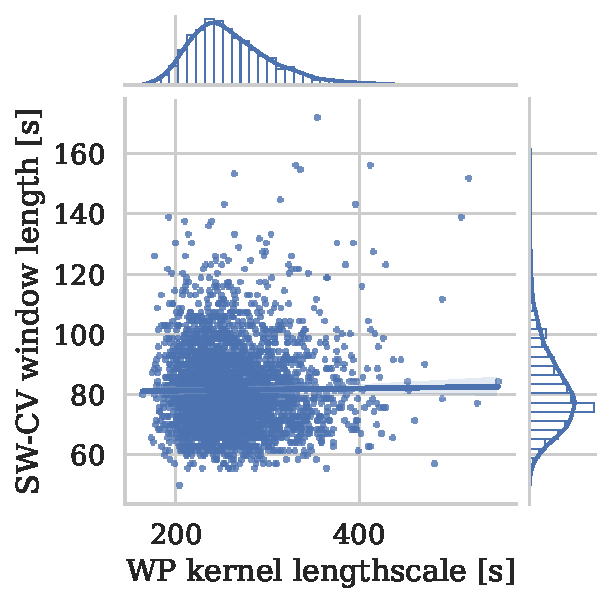
\includegraphics[width=0.45\textwidth]{fig/hcp/d15/lengthscale_optimal_window_length_relations}
  \caption{
    HCP benchmark relationship between learned SVWP kernel lengthscales (scaled to time series length) and SW-CV optimal window length.
    Each dot represents one of four scans (1A, 1B, 2A, 2B) for each subject.
    Full time series are 864 seconds long.
  }\label{fig:sim-relationship-lengthscale-optimal-window-length}
\end{figure}


As we see that the \gls{svwp} and \gls{sw-cv} estimates are distinct in this case, we compare the learned \gls{svwp} kernel lengthscales with the estimated optimal window lengths (similar to \cref{fig:sim-optimal-window-lengths} and \cref{fig:sim-learned-kernel-lengthscales}).
Perhaps surprisingly, despite prior evidence that these two hyperparameters may pick up on similar aspects of the data, we do not find a significant relationship between them here across all scans, as shown in \cref{fig:sim-relationship-lengthscale-optimal-window-length}.
One explanation for this could be that these learned hyperparameters are mostly related to the variance summary measure (where \gls{svwp} and \gls{sw-cv} estimates are quite distinct) rather than the rate-of-change summary measure (where they are more similar).
Alternatively, it may be the case that with the simulations the covariance structures were much more distinct, whereas in this actual data set the dynamics between edges may not differ as much.
These two hyperparameters may still correspond to each other, but these results suggest caution.

%%
\subsubsection{Subject measure prediction benchmark}
%%


\begin{figure}[t]
  \centering
  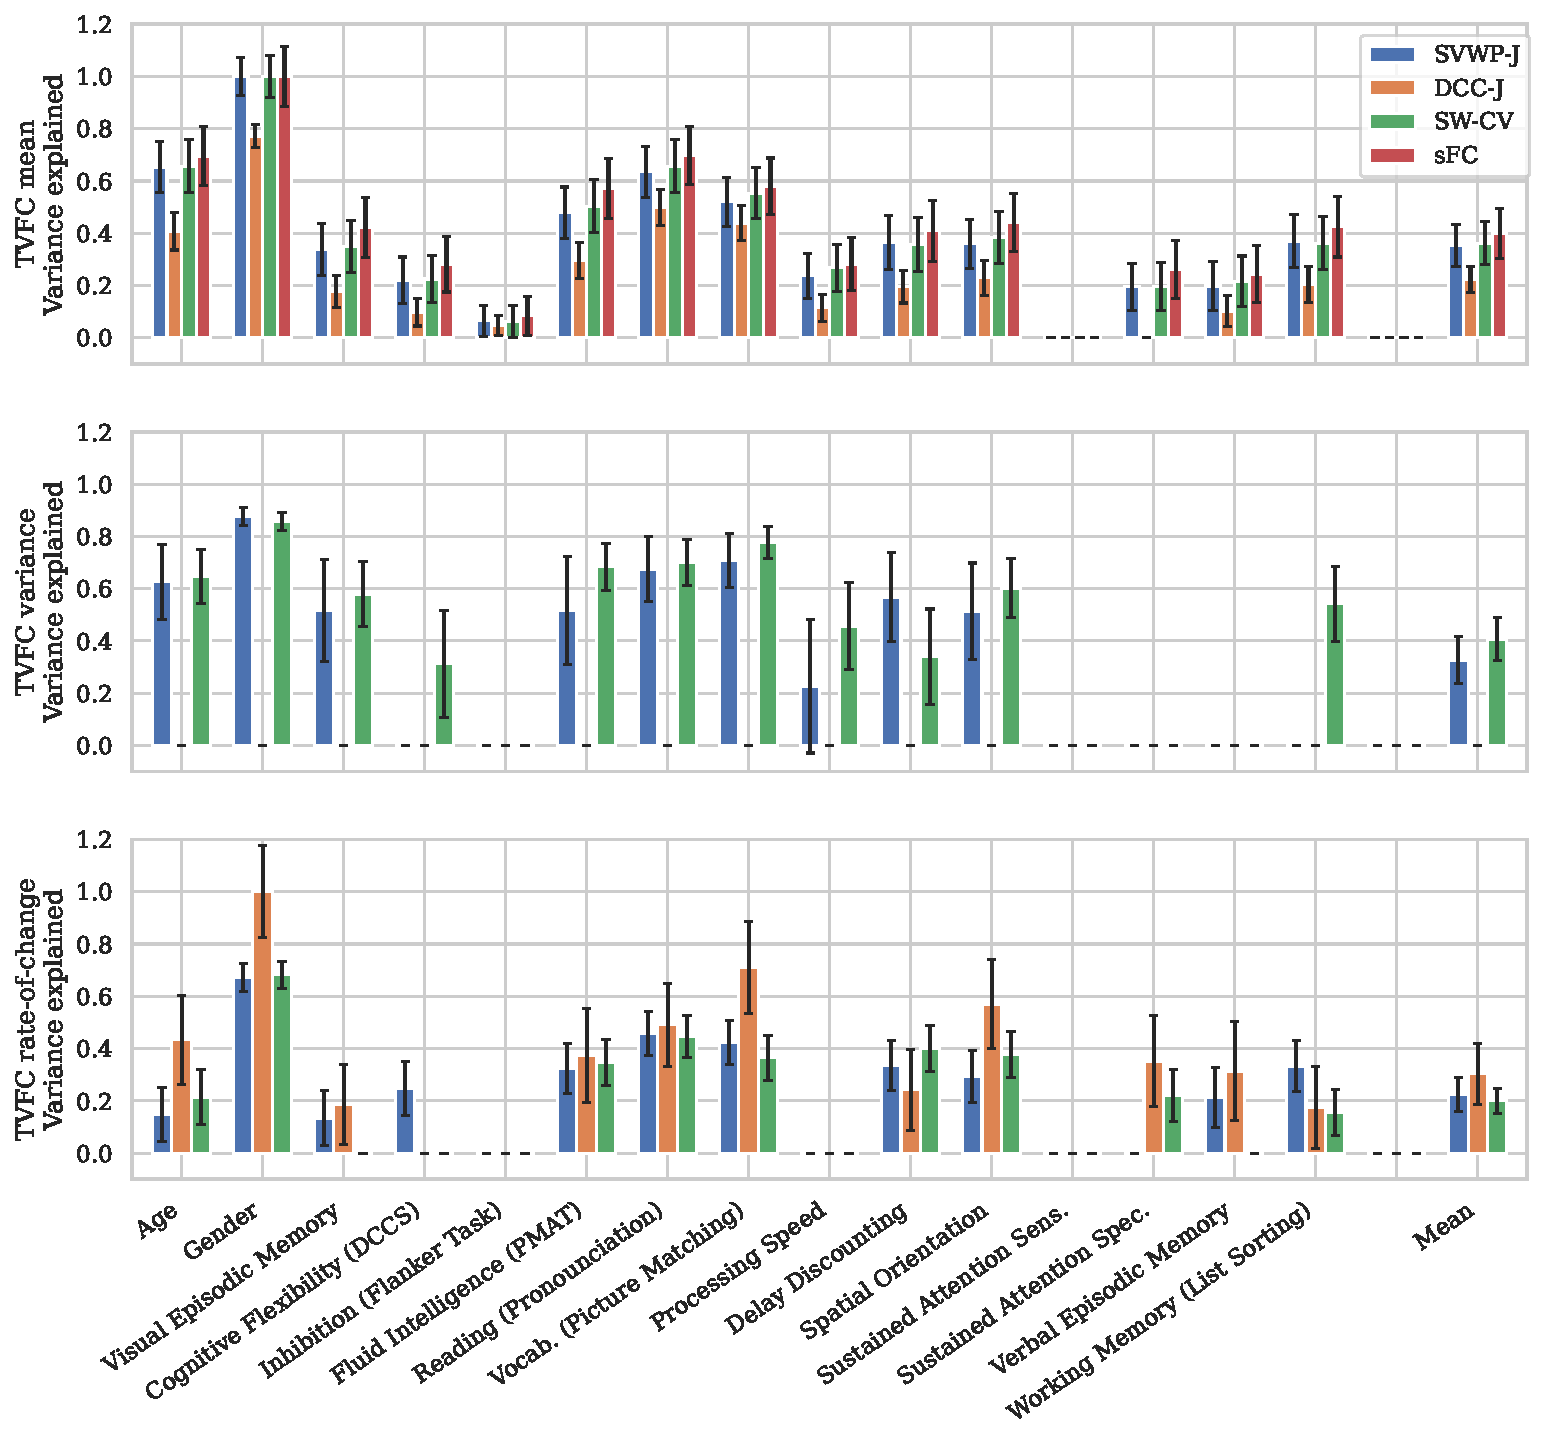
\includegraphics[width=\textwidth]{fig/hcp/d15/subject_measure_prediction/cognitive/morphometricity_all_TVFC_summary_measures}
  \caption{
    HCP benchmark subject cognitive measures prediction morphometricity scores (with standard error).
    Run on TVFC summary measures of mean (top), variance (middle), and rate-of-change (bottom row).
    sFC is added for reference to the TVFC mean plot.
  }\label{fig:hcp-results-subject-measures-prediction}
\end{figure}


Morphometricity (variance explained) scores are shown in \cref{fig:hcp-results-subject-measures-prediction}.
The pairwise \gls{dcc} scores are almost identical to the joint \gls{dcc}, which is unsurprising as the summary measures are almost identical.
Hence, they are left out here.
%
Since we study the same subject measures as \textcite{Li2019a}, we can compare the \gls{sfc} (as a reference or \emph{null} model; the alternative hypothesis that \gls{fc} is static) and \gls{tvfc} estimate means (top row) directly to theirs.
Scores are generally replicated, for example being close to 1 (for all methods) for Gender.
This provides a healthy sanity check.
%
We also see that none of the \gls{tvfc} estimation methods can outperform the \gls{sfc} method regarding mean \gls{fc} (connectivity strength).
This was expected and highlights that we should only look at \gls{tvfc} methods if we are interested in brain connectivity \emph{dynamics}.
However, a good \gls{tvfc} estimation method should still model mean \gls{tvfc} well (i.e.~get as close to \gls{sfc} performance as possible).

We observe several things from these results.
%
First, for some subject measures none of the variance across all \gls{tvfc} summary measures and estimation methods can be explained (see e.g.~Sustained Attention Sens.).
This could indicate that signatures of these respective tasks are not captured by \gls{fc} in general.
%
Second, we observe strong heterogeneity across methods.
There is no clear-cut conclusion on picking a superior method here.
A method may outperform another on one occasion, but not on another.
However, overall the \gls{svwp} and \gls{sw-cv} methods perform best, whereas \gls{dcc} often fails to explain much variance across these measures.\footnote{As another validation of cross-validating window lengths, we ran the \gls{sw} approach with a window length of both 30 and 60 seconds. The \gls{sw-cv} estimates consistently outperformed both of these, even as this would be an unfair, post-hoc comparison.}
Particularly noteworthy is the complete lack of the \gls{dcc} \gls{tvfc} variance estimates to have any predictive power.
This can be interpreted as it being meaningless (which we will later see to be relevant for the test-retest benchmark).
%
In general, it is also promising here that the time-varying summary measures (variance and rate-of-change) contain information about subject measures as well.
This highlights the value of studying \gls{fc} dynamics instead of merely its properties over the full scan.
%
Another observation can be made about how subject measures are expressed.
In fact, this helps us understand what these summary measures capture.
Subject age, for example, seems to affect \gls{tvfc} mean and variance more so than rate-of-change.
Such insights could lead to (careful) biophysical interpretations as well.
For example, \textcite{Hutchison2015} found that \gls{fc} variability over the length of a scan correlates positively with age.
Based on this finding, we would expect \gls{tvfc} variance to be predictive of age (to some degree).
We do indeed find this for the \gls{wp} and \gls{sw-cv} methods but fail to find this for the \gls{dcc} method.
Such comparisons to literature can be used to assess the validity and general usefulness of a \gls{tvfc} estimation method.
%
Finally, we see that the performance of \gls{svwp} and \gls{sw-cv} estimates are generally coordinated (performing well and failing in similar contexts).
This aligns with our prior intuition that these methods may capture similar aspects of the data.


\begin{figure}[t]
  \centering
  \subcaptionbox{SVWP-J\label{fig:test-retest-mean-SVWP-ICCs}}{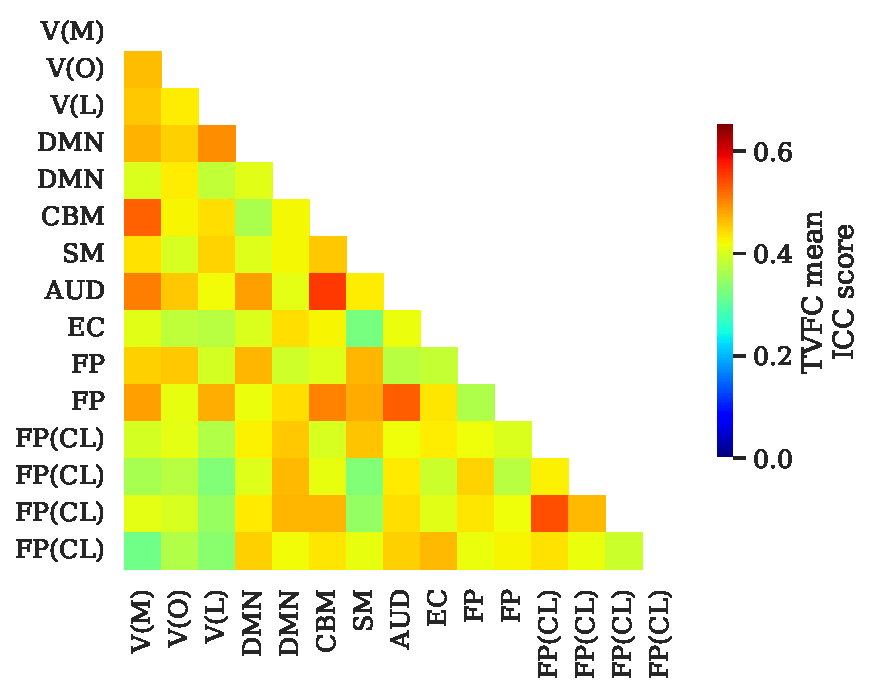
\includegraphics[width=0.28\textwidth]{fig/hcp/d15/test_retest/ICCs/correlation_mean_ICCs_SVWP_joint}}
  \subcaptionbox{DCC-J\label{fig:test-retest-mean-DCC-ICCs}}{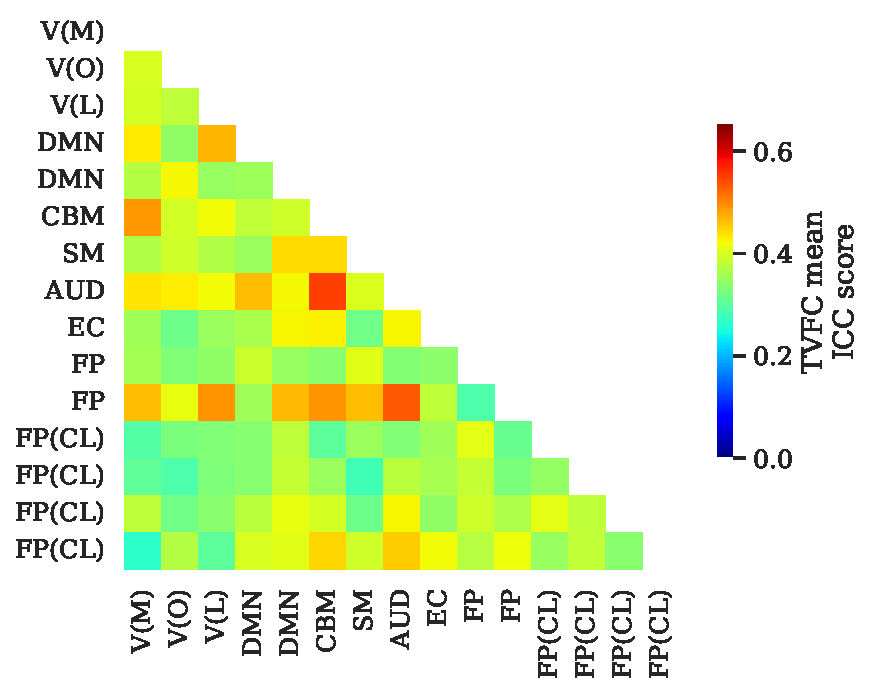
\includegraphics[width=0.28\textwidth]{fig/hcp/d15/test_retest/ICCs/correlation_mean_ICCs_DCC_joint}}
  \subcaptionbox{SW-CV\label{fig:test-retest-mean-SW-ICCs}}{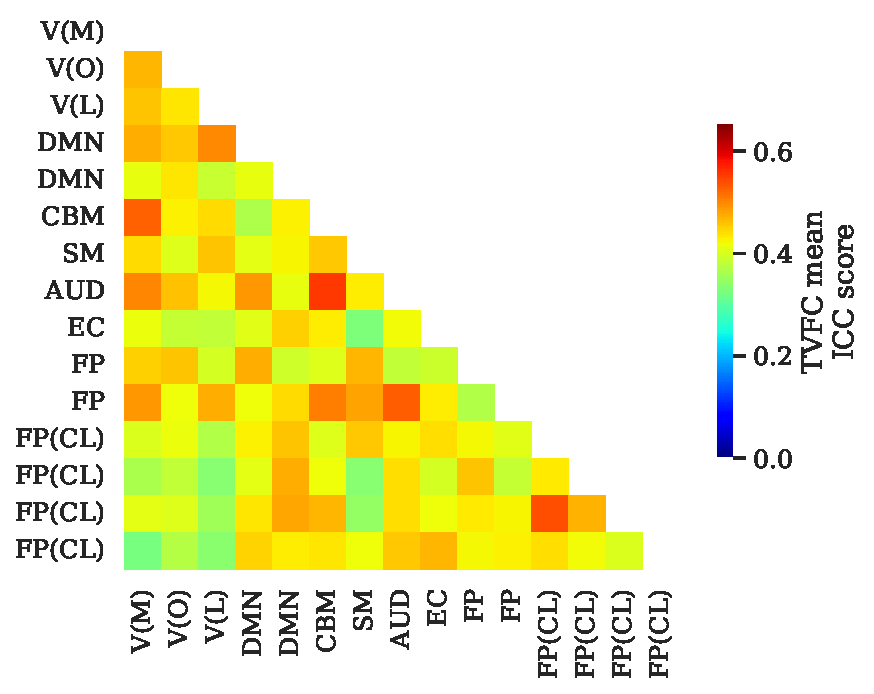
\includegraphics[width=0.28\textwidth]{fig/hcp/d15/test_retest/ICCs/correlation_mean_ICCs_SW_cross_validated}}
  \subcaptionbox{SVWP-J\label{fig:test-retest-variance-SVWP-ICCs}}{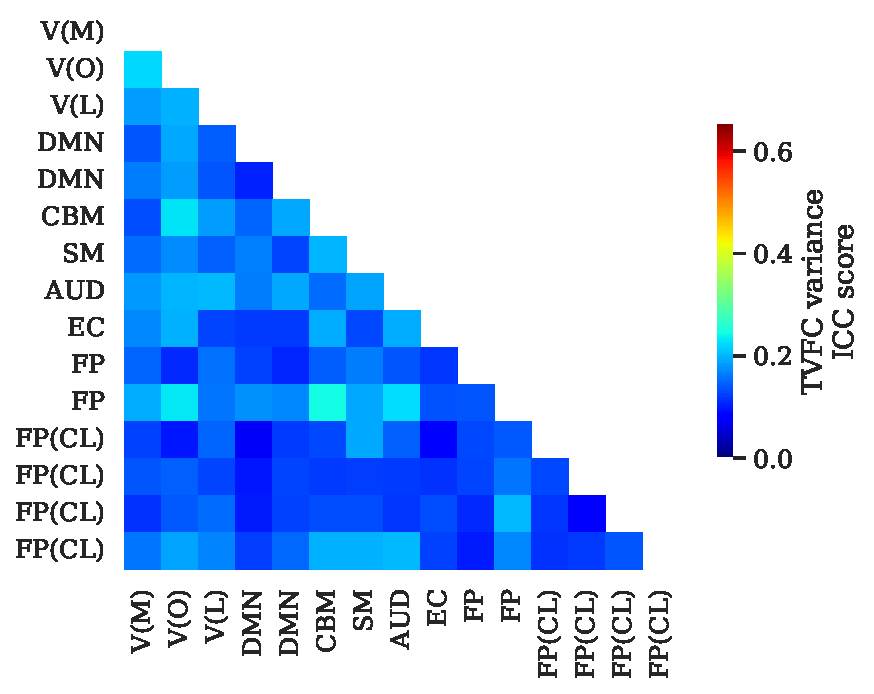
\includegraphics[width=0.28\textwidth]{fig/hcp/d15/test_retest/ICCs/correlation_variance_ICCs_SVWP_joint}}
  \subcaptionbox{DCC-J\label{fig:test-retest-variance-DCC-ICCs}}{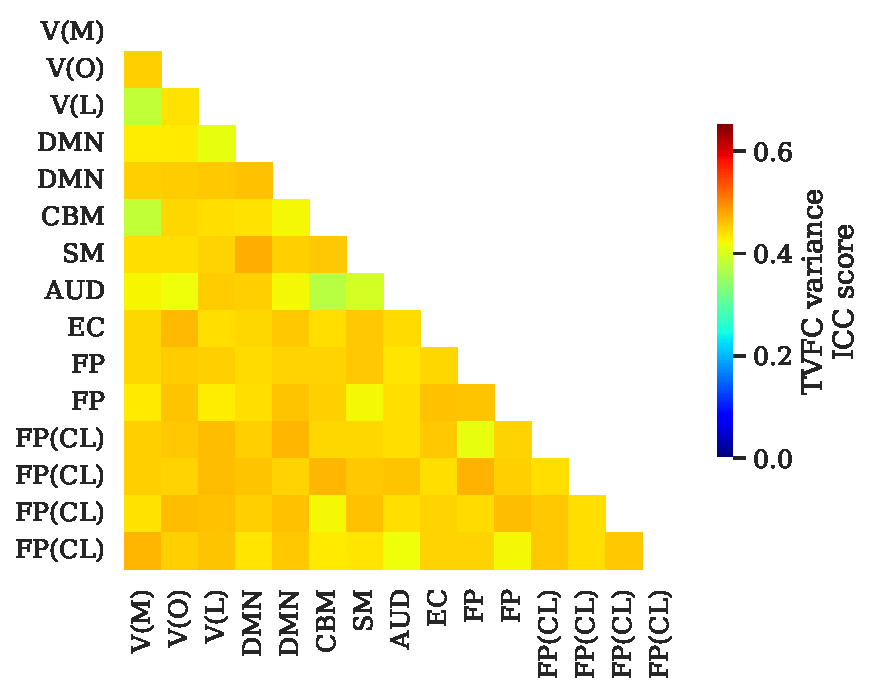
\includegraphics[width=0.28\textwidth]{fig/hcp/d15/test_retest/ICCs/correlation_variance_ICCs_DCC_joint}}
  \subcaptionbox{SW-CV\label{fig:test-retest-variance-SW-ICCs}}{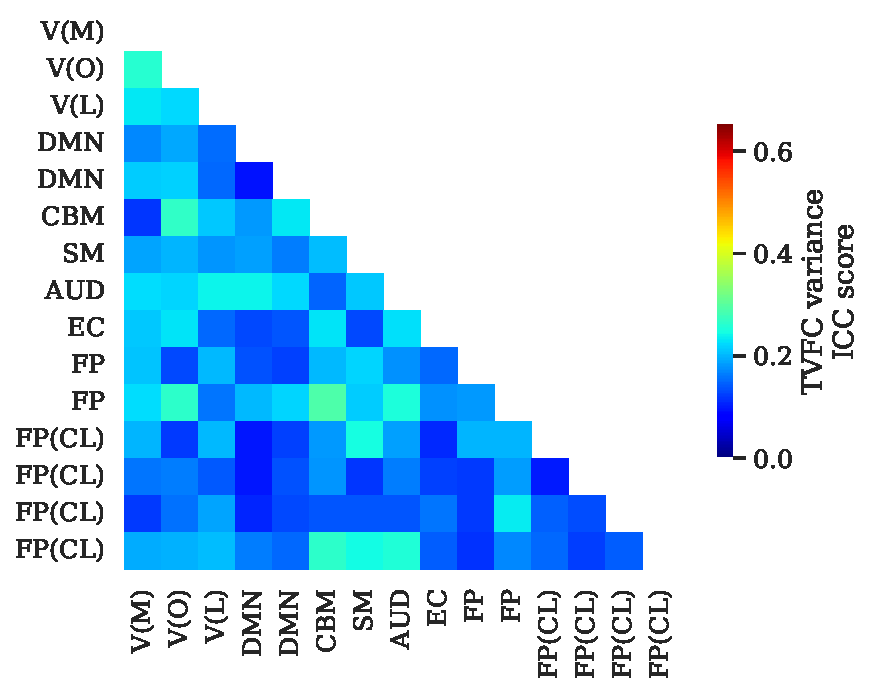
\includegraphics[width=0.28\textwidth]{fig/hcp/d15/test_retest/ICCs/correlation_variance_ICCs_SW_cross_validated}}
  \subcaptionbox{SVWP-J\label{fig:test-retest-roc-WP-ICCs}}{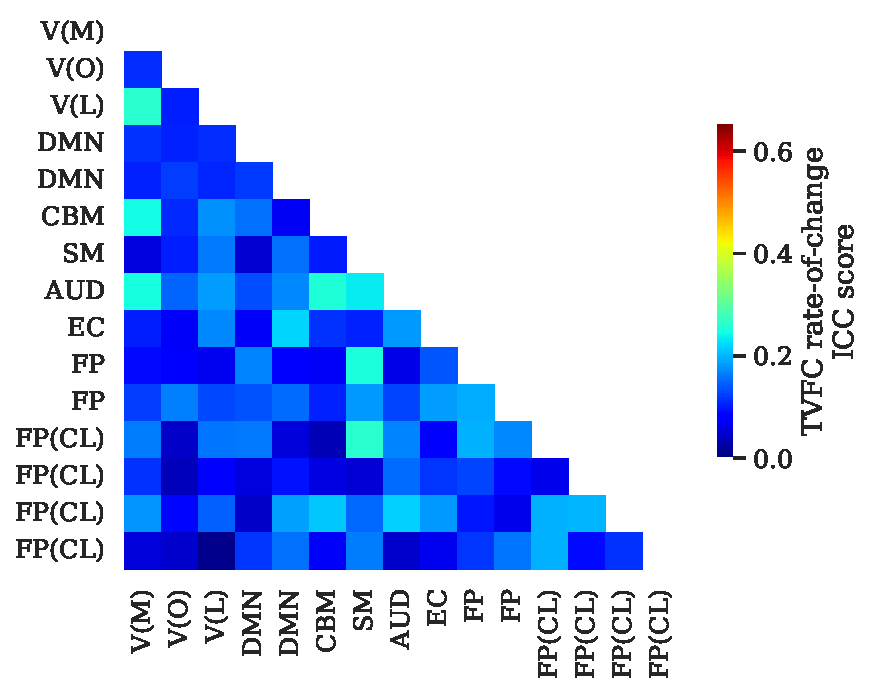
\includegraphics[width=0.28\textwidth]{fig/hcp/d15/test_retest/ICCs/correlation_rate_of_change_ICCs_SVWP_joint}}
  \subcaptionbox{DCC-J\label{fig:test-retest-roc-DCC-ICCs}}{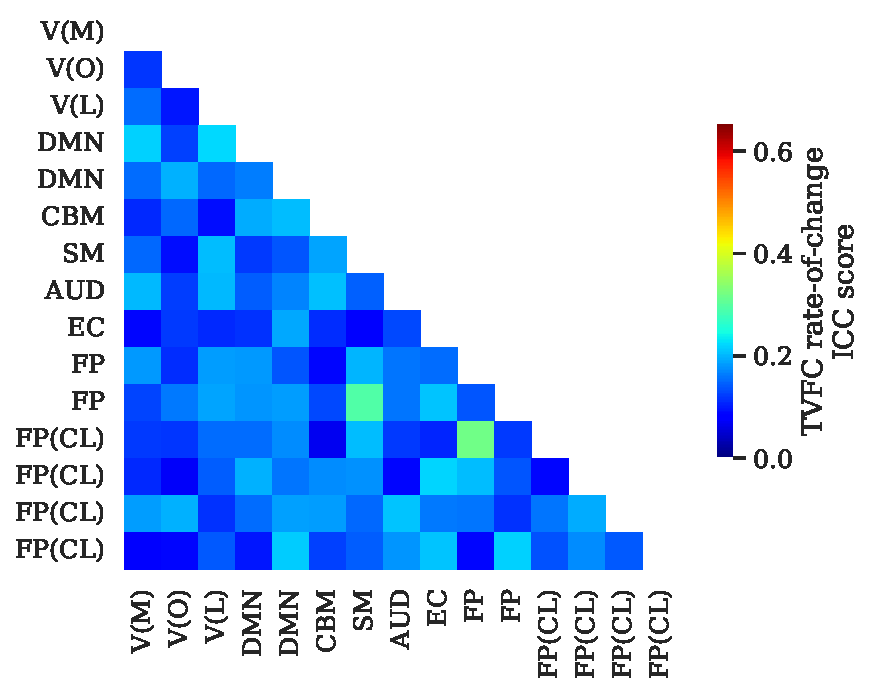
\includegraphics[width=0.28\textwidth]{fig/hcp/d15/test_retest/ICCs/correlation_rate_of_change_ICCs_DCC_joint}}
  \subcaptionbox{SW-CV\label{fig:test-retest-roc-SW-ICCs}}{\includegraphics[width=0.28\textwidth]{fig/hcp/d15/test_retest/ICCs/correlation_rate_of_change_ICCs_SW_cross_validated}}
  \caption{
    HCP benchmark test-retest robustness edgewise ICC(2,1) scores across four scans of estimated TVFC on $D = 15$ ICA-based data.
    Reliability of TVFC means (top), variance (middle), and rate-of-change (bottom row) are shown.
    For interpretation, ICA components are mapped to FNs.
    Visual (V): medial (M), occipital (O), lateral (L); Default Mode Network (DMN); Cerebellum (CBM); Sensorimotor (SM); Auditory (AUD); Executive Control (EC); Frontoparietal (FP) with Cognition-Language (CL) subset.
  }\label{fig:hcp-results-test-retest-ICCs-d15}
\end{figure}


\info[inline]{Paragraph: Discuss additional subject measures.}
Morphometricity scores for additional subject measures (including social-emotional and other measures) can be found in \cref{appendix:hcp-more-results}.
The variance explained for these measures is generally much lower.
This shows that \gls{fc} may capture cognitive individual differences better than affective ones.
Comparing to prior findings, we replicate \textcite{Dubois2018} and find that the Big Five personality trait of `openness to experience' is best explained by \gls{sfc}~\parencite[see also][]{Beaty2018}.

This morphometricity analysis is based on a linear model.
To understand more complex dynamics captured by the various methods, we may need to run models such as \glspl{rnn}.
If we are solely interested in making subject measure predictions, we could also bypass covariance structure estimation entirely.
However, we reiterate that our goal here is not to build the best model for subject measure prediction, but to benchmark \gls{tvfc} estimation methods.

%%
\subsubsection{Test-retest robustness benchmark}
%%

The \gls{icc} scores per edge are shown in \cref{fig:hcp-results-test-retest-ICCs-d15}, analogous to figures 4B and 4C in \textcite{Choe2017}.
Each \gls{ica} component is labeled with one of the 10 BrainMap components from \textcite{Smith2009} with most overlap (see \cref{fig:brainmap-functional-networks}).
%
Some edges are shown to be more robust than others, consistently across methods (see e.g.~CBM-AUD).
However, this increased robustness does not generalize across summary measures.
Furthermore, \gls{dcc} mean \gls{tvfc} edges are slightly less robust than the other methods, but its variance is much more robust.
This outperformance over \gls{sw} methods was found by \textcite{Choe2017} too.
Overall, robustness of connectivity strengths is much higher than for the dynamic summary measures.

The omnibus (whole brain) I2C2 scores for the reliability of the \gls{tvfc} mean, variance, and rate-of-change are shown in \cref{fig:hcp-results-test-retest-I2C2-scores-d15}.
Just like \textcite{Choe2017}, we do not find much disagreement between \gls{icc} and I2C2 scores.
The I2C2 score is a good representation of the ``average'' \gls{icc} score over all edges from \cref{fig:hcp-results-test-retest-ICCs-d15}.
We posit that using I2C2 scores is a good measure for whole-brain test-retest robustness.
However, in some cases we may be interested in the robustness of particular edges.
For comparison, \textcite{Choe2017} found respective values for the \gls{tvfc} mean between 0.44 and 0.48 for all methods.
We find similar values for all our methods.
They found respective values for the \gls{tvfc} variance between 0.16 and 0.30 for \gls{sw} methods (with different window lengths) and 0.49 for \gls{dcc}.
That is, they also found more variety between methods in I2C2 values for \gls{tvfc} variances than for \gls{tvfc} means.


\begin{figure}[t]
  \centering
  \includegraphics[width=\textwidth]{fig/hcp/d15/test_retest/I2C2/correlation_I2C2_scores}
  \caption{
    HCP benchmark test-retest robustness I2C2 omnibus scores for mean, variance, and rate-of-change TVFC summary measures.
  }\label{fig:hcp-results-test-retest-I2C2-scores-d15}
\end{figure}


Following up from \cref{subsec:model-features}, we can also compute the \gls{icc} score for the learned \gls{svwp} kernel parameters.
We find a score of 0.29 for the kernel variance and 0.48 for the kernel lengthscales $l$.
Taking the categories from \textcite{Cicchetti1994}, these can be considered `poor' and `fair', respectively.
These are high in comparison to the scores for the summary measures.
%
How should we interpret these results?
From the perspective of viewing this as a prediction problem, we can view this test-retest problem as the following question: ``Given the first scan, how well can we predict which scan is that subject's subsequent scan?''.
The issue here is not just to look at test-retest scores, but to use them to justify using one method over another.
In that light, we just expect a method to generate \emph{any} feature that may help us do this.
The method with the best score from any such feature can be considered stronger.
%
Furthermore, it is not clear how having more robust estimations across scans is related to actual performance on subsequent tasks.
We will discuss this point more in \cref{subsec:benchmarking-discussion-rs-fmri}.

%%
\subsubsection{Imputation benchmark}
%%

Results for the imputation study are shown in \cref{fig:hcp-results-LEOO-multivariate}.
Shown are results under the \gls{leoo} train and test set creation.
The \gls{wp} and \gls{sw-cv} methods outperform the other methods.
The poor performance of \gls{dcc} here may be due to not learning the correct mean.


\begin{figure}[t]
  \centering
  \includegraphics[width=\textwidth]{fig/hcp/d15/imputation_study/LEOO_multivariate_test_log_likelihoods_raincloud}
  \caption{
    HCP benchmark imputation results under LEOO train-test split.
    The boxplot shows median, quartiles, and outliers.
  }\label{fig:hcp-results-LEOO-multivariate}
\end{figure}


\begin{figure}[t]
  \centering
  \subcaptionbox{SVWP-J\label{fig:edgewise-imputation-benchmark-SVWP}}{\includegraphics[width=0.45\textwidth]{fig/hcp/d15/imputation_study/LEOO_multivariate_test_log_likelihoods_edgewise_SVWP_joint}}
  \subcaptionbox{DCC-J\label{fig:edgewise-imputation-benchmark-DCC}}{\includegraphics[width=0.45\textwidth]{fig/hcp/d15/imputation_study/LEOO_multivariate_test_log_likelihoods_edgewise_DCC_joint}}
  \subcaptionbox{SW-CV\label{fig:edgewise-imputation-benchmark-SW-CV}}{\includegraphics[width=0.45\textwidth]{fig/hcp/d15/imputation_study/LEOO_multivariate_test_log_likelihoods_edgewise_SW_cross_validated}}
  \subcaptionbox{sFC\label{fig:edgewise-imputation-benchmark-STATIC}}{\includegraphics[width=0.45\textwidth]{fig/hcp/d15/imputation_study/LEOO_multivariate_test_log_likelihoods_edgewise_sFC}}
  \caption{
    HCP benchmark edgewise imputation results for various methods on $D = 15$ ICA-based data.
    The equivalent of mean test log likelihoods from \cref{fig:hcp-results-LEOO-multivariate} are shown for each edge individually.
    For interpretation, ICA components are mapped to FNs.
    Visual (V): medial (M), occipital (O), lateral (L); Default Mode Network (DMN); Cerebellum (CBM); Sensorimotor (SM); Auditory (AUD); Executive Control (EC); Frontoparietal (FP) with Cognition-Language (CL) subset.
  }\label{fig:hcp-results-edgewise-imputation-benchmark}
\end{figure}


This is a whole-brain analysis.
However, there may be certain edges where \gls{svwp} performance is similar to the static approach (i.e.~static edges) and some where it outperforms (i.e.~dynamic edges).
In fact, we posit that outperformance over static estimates can be considered a proxy for a statistical test of whether there is any time-varying structure~\parencite[see also][]{Zalesky2014, Hindriks2016}.
This point was made earlier based on \cref{fig:sim-imputation-study-d2-null,fig:sim-imputation-study-d2-periodic-1}.
To further explore this proposal, the population-level edgewise imputation benchmark scores (averaged over all subjects) are plotted in \cref{fig:hcp-results-edgewise-imputation-benchmark}.
First, caution is advised when interpreting these.
Certain edges have high performance on this imputation benchmark, see e.g.~FP-FP(CL), but this may simply be due to this edge being very static (and thus easier to fit).
Comparison between edges is less insightful than comparison for the same edge \emph{between} estimation methods.
%
We find \gls{svwp} outperformance over \gls{sfc} is stronger in certain edges.
This may point to these edges changing more across time.
And indeed, these edges have higher variance and rate-of-change summary measures (see \cref{fig:HCP-model-estimates-summary-measures-var-SVWP,fig:HCP-model-estimates-summary-measures-roc-SVWP}).

%%
\subsubsection{Brain state analysis}
%%

Extracted brain states for \gls{svwp}, \gls{dcc}, and \gls{sw-cv} are shown in \cref{fig:hcp-results-brain-states-svwp,fig:hcp-results-brain-states-dcc,fig:hcp-results-brain-states-sw-cv}, respectively.
Interestingly, the extracted brain states for \gls{svwp} and \gls{sw-cv} estimates look similar.
The first brain state also looks like the \gls{sfc} estimates, as expected~\parencite{Allen2014}.

Apart from the extracted brain states, we are also interested in the dynamics and transitions of brain states.
The number of brain state change points per method per subject is shown in \cref{fig:hcp-brain-state-change-point-counts}.
Our intuition from \cref{fig:hcp-model-estimates-example} is confirmed; \gls{sw-cv} predicts many more brain state switches than \gls{svwp} (even though the state centroids are similar).
Furthermore, we see that the spread across subjects is large for \gls{dcc}, with many subjects having no change points and others a great many.


\begin{figure}[t]
  \centering
  \includegraphics[width=\textwidth]{fig/hcp/d15/brain_states/k03/brain_state_switch_count}
  \caption{
    HCP brain state analysis number of brain state change points per TVFC estimation method.
    Total number of time points is $N = 1200$.
    Run on multivariate (all $D = 15$ time series) HCP data.
    The boxplot shows median, quartiles, and outliers.
  }\label{fig:hcp-brain-state-change-point-counts}
\end{figure}


%%
\subsection{Task-based fMRI}\label{subsec:rockland-results}
%%

First, we compare the \gls{vwp} kernel lengthscales to the optimal learned window length again, shown in \cref{fig:rockland-relationship-lengthscale-optimal-window-length}.
We do not find a relationship between the two.
This may indicate a failure of one (or both) of these methods to capture anything meaningful, or the approaches to focus on distinct aspects of the data.
Alternatively, these hyperparameters may in fact not be crucial to the estimates, these being driven much more by the actual observations.


\begin{figure}[t]
  \centering
  \includegraphics[width=0.45\textwidth]{fig/rockland/CHECKERBOARD645/lengthscale_optimal_window_length_relations}
  \caption{
    Rockland benchmark relationship between learned VWP kernel lengthscales (scaled to time series length) and SW-CV optimal window length.
    Each dot represents one of 286 Rockland subjects.
    Full time series is 154.8 seconds long.
  }\label{fig:rockland-relationship-lengthscale-optimal-window-length}
\end{figure}


We start with a visual inspection of model \gls{tvfc} estimates, shown in \cref{fig:rockland-results-tvfc-predictions}.
Just like the node time series plot, since we have an external task, we can average estimates across all subjects.


\begin{figure}[ht]
  \centering
  \includegraphics[width=\textwidth]{fig/rockland/CHECKERBOARD645/TVFC_predictions/all_subjects_joint_correlations}
  \caption{
    Rockland benchmark model TVFC estimates.
    Shaded areas indicate presence of external visual stimulus.
    Average estimates over all 286 subjects.
  }\label{fig:rockland-results-tvfc-predictions}
\end{figure}


As discussed, we expect that correlation between \gls{v1} and other regions should decrease as we move up and away from the visual cortex hierarchy.
We do in fact observe this from all models: connectivity with V2 is highest, followed by V3, V4, \gls{mpfc}, and connectivity strength with \gls{m1} is lowest.
However, the mean \gls{tvfc} is quite different across estimation methods, and often quite different from the \gls{sfc} estimate.
This also highlights how important the choice of \gls{tvfc} estimation method can be.

%%
\subsubsection{External stimuli prediction}
%%

Extracted $\textbf{\beta}$ parameters from our \gls{glm} are shown in \cref{fig:rockland-results-glm-betas}.
%
As expected, the \gls{sfc} cannot capture any time-varying structure.
Therefore, all drift parameters, as well as weights for task-related regressors are set to zero.
Instead, the full \gls{sfc} estimates are captured by the constant (offset) parameter of the design matrix.
%
In terms of other models, we see the \gls{vwp} model having the largest estimated task-related $\textbf{\beta}$ parameters.
Interestingly, the within-visual cortex edges have the most predictive power.
As expected from the visual inspection, the \gls{glm} has removed negative trends for \gls{v1}--\gls{mpfc} and \gls{v1}--\gls{m1}.
We conclude that the \gls{vwp} estimates have captured the most of the external task.


\begin{figure}[ht]
  \centering
  \subcaptionbox{VWP-J\label{fig:rockland-results-glm-betas-VWP}}{\includegraphics[width=0.48\textwidth]{fig/rockland/CHECKERBOARD645/prediction_benchmark/GLM_beta_VWP_joint}}
  \subcaptionbox{DCC-J\label{fig:rockland-results-glm-betas-DCC}}{\includegraphics[width=0.48\textwidth]{fig/rockland/CHECKERBOARD645/prediction_benchmark/GLM_beta_DCC_joint}}
  \subcaptionbox{SW-CV\label{fig:rockland-results-glm-betas-SW-CV}}{\includegraphics[width=0.48\textwidth]{fig/rockland/CHECKERBOARD645/prediction_benchmark/GLM_beta_SW_cross_validated}}
  \subcaptionbox{sFC\label{fig:rockland-results-glm-betas-sFC}}{\includegraphics[width=0.48\textwidth]{fig/rockland/CHECKERBOARD645/prediction_benchmark/GLM_beta_sFC}}
  \caption{
    Rockland benchmark GLM $\beta$ (beta) parameters per TVFC estimation method.
    Values indicate learned weights.
    Higher values indicate that the GLM uses the respective design matrix features more.
    The VWP TVFC estimates are most useful for predicting the presence of the external stimulus (rest and stim columns).
  }\label{fig:rockland-results-glm-betas}
\end{figure}


%%
\subsubsection{Imputation benchmark}
%%

The imputation benchmark results (\cref{fig:rockland-results-imputation-benchmark}) show strong performance for the \gls{vwp} model and weak performance for \gls{dcc}.
\gls{sw-cv} estimate likelihoods are similar to \gls{sfc} estimates.
This may have been expected based on the visual inspection of model estimates; the \gls{sw-cv} approach found the right mean but failed to capture the dynamics.
%
As such, we show strong correspondence of performance on the imputation benchmark with the external task prediction benchmark.


\begin{figure}[ht]
  \centering
  \includegraphics[width=\textwidth]{fig/rockland/CHECKERBOARD645/imputation_study/LEOO_test_log_likelihoods_raincloud}
  \caption{
    Rockland benchmark imputation results under LEOO train-test split.
    Run on~286~Rockland data subjects.
    The boxplot shows median, quartiles, and outliers.
  }\label{fig:rockland-results-imputation-benchmark}
\end{figure}

\clearpage
\section{Discussion}
%%%%%

The aim of this chapter was to convince ourselves what the best approach for estimating \gls{tvfc} is.
How well did we succeed in that?

%%
\subsection{Simulations}
%%

In summary, we studied simulated time series defined by a range of edge case and (possibly) realistic covariance structures.
We took advantage of the flexibility simulations bring, and studied the impact of data dimensionality and noise configurations.
These simulation benchmarks have taught us the following.

Firstly, we found that \gls{sw-cv} and its ability to find an appropriate window length works well.
The \gls{wp} approaches learn kernel lengthscales $l$ as a hyperparameter, and it seems to have a similar function as the window length.
%
Furthermore, we have replicated the frequent observation that standard \gls{sw} approaches can produce spurious correlation structures if the underlying covariance structure is actually static.
Caution is required to avoid false positive conclusions.
We also saw that \gls{dcc} models can still yield these.
%
The \gls{wp} approach generally works well, but may smooth out the estimates too much.
We also see that all models perform poorly on the `state transition' data set.
As such we learned that if we expect to see drastic sudden changes in covariance structure, the current approaches may all be insufficient.
%
Quantifying our results, we see the \gls{wp} model outperforming the others in most cases.
Combined with the additional qualitative benefits of this model, uncertainty modeling for example, we have established its promise for application in neuroimaging.
%
Lastly, we found all results to be broadly robust to data dimensionality and noise characteristics.

However, these results cannot be considered conclusive, because we still do not know what covariance structures can be found in real data.
Are they transient or spike-like point processes consisting of state transition events?
These simulation benchmarks can certainly rule out some methods, but do not paint a full picture.
%
To dive deeper, we needed to investigate method estimates on real data.
The closer our benchmarks are to actual practical applications, the more valuable they will be.
For example, we do not actually know if it matters if a method's estimates are more `noisy' (see \gls{dcc} estimates for periodic covariance structures).
Perhaps capturing general trends is good enough for most practical scenarios.

%%
\subsection{Resting-state fMRI}
\label{subsec:benchmarking-discussion-rs-fmri}
%%

In summary, we studied several popular types of \gls{rs-fmri} benchmarks on a single, large, and publicly available data set.
These benchmarks have taught us the following.

Firstly, we find large qualitative differences in the \gls{tvfc} estimates between different estimation methods.
But how relevant are these?
%
The \gls{rs-fmri} benchmarks have taught us that choice of \gls{tvfc} estimation method greatly affects the utility of these estimates to predict subject measures.
In general, we find the \gls{svwp} and \gls{sw-cv} methods to do similarly well.
However, each has different predictive power for different subject measures and different qualitative characteristics.
%
In terms of the test-retest studies, the results are harder to interpret.
All methods seem to do relatively similarly here, but \gls{dcc} estimate variances are much more robust across scanning sessions.
In fact, the utility of test-retest studies in general is questionnable.
It is unclear if we want to pick up on reliable characteristics or those that are indicative of cognitive occupation during a scan.
Test-retest reliability may be desired, but optimizing for it for its own sake misses the point.
Underwriting this, in a recent opinion piece \textcite{Finn2021b} also argued that (behaviorally) \emph{predictive} connectomes are more important than reliable connectomes.
%
In terms of the imputation benchmark, we find performance to be related to subject measure prediction performance.
This again confirms its promise as benchmark in situations where no ground truth is available.
%
Lastly, the brain state analysis demonstrated that \gls{tvfc} estimation method choice impacts not only the brain states extracted, but also related metrics such as switch rates.

%%
\subsection{Task-based fMRI}
%%

In summary, we used an \gls{tb-fmri} data set with external visual task to induce a covariance structure in individuals, which was attempted to be reconstructed.

Unlike the simulations and \gls{rs-fmri} benchmarks, this \gls{tb-fmri} benchmark has a clear winner.
None of the methods except the \gls{vwp} was able to recover (some of) the external stimulus presence.

However, this data set may be too simple in some sense, and not representative of realistic stimuli humans experience.
Other \gls{tb-fmri} with richer task structure could be added to these benchmarks.
For example, \textcite{Xie2019} studied classification accuracy in a multi-task setting data set, where the external stimulus again was used as a proxy for ground truth.

%%
\subsection{Reflection on benchmarking}
\label{subsec:benchmarking-reflection}
%%

What have we learned from these benchmarks?
%
We have not only proposed novel ways of estimating \gls{tvfc}, but also motivated and demonstrated how to think about robustly estimating it: by framing and designing benchmarks as prediction problems.

Overall we consider the \gls{wp} to perform well, and best among these methods considered.
%
Having the benchmarking framework in place also allows us to make model adjustments and rapidly check if these improved performance.
Ideas for model extensions will be discussed in \cref{subsec:model-extensions}.

Equally insightful and encouraging is that the imputation benchmark generally corresponds to estimation method performance on the concurrent benchmark.
Given such a strong relationship between performance on this benchmark and the more informative benchmark, researchers may decide on which \gls{tvfc} estimation method to use in practice by running the imputation benchmark on their data set at hand.
This is the beauty of the imputation benchmark: it uses real data and thus a real ground truth, and it can be run on any data set without the need for expert labeling or concurrent information.

%%
\subsubsection{Sudden changes and change points}
\label{subsec:sudden-changes}
%%

One of the open questions brought to the fore in this thesis concerns \gls{tvfc} change points.
We must still consider the possibility of real covariance structures to be organized in change points, for which additional benchmarks need to be designed.
This is one of the biggest gaps in the framework at the moment.

It is often assumed that covariance between two brain regions can change and switch rapidly.
The prior of the \gls{wp} is that covariance changes slowly.
As we have seen, none of the proposed models are actually capable of picking up on sudden changes in covariance structure.
Therefore, the real question is whether such jumps can be expected in real data.
As argued by~\textcite{Lindquist2014} as well, if we expect sudden changes in our structure, we may need a different class of models.
Another probabilistic approach to modeling \gls{tvfc} was also not able to capture the jagged dynamics of discrete jumps and states~\parencite{Li2019b}.

Change point detection algorithms can help determine whether such sudden changes exist.
There is a whole literature on modeling brain state change points or switches directly from data~\parencite[see e.g.][]{Robinson2010, Cribben2012, Cribben2013, Lindquist2014, Ou2014, Xu2015, Kim2021, Anastasiou2022}.
We may take inspiration from \textcite{Saatci2010, Wilson2013} on change point kernels to include in the \gls{wp} models.

Other types of neuroimaging data, such as local field potential time series data, often include outliers.
If such outliers cannot be discarded as anomalies, but are expected under the scientific framework to be biologically insightful, this limits methods such as the \gls{wp}.

%%
\chapter{TVFC and depression}
\label{ch:ukb}
%%%%%

\info[inline]{Paragraph: Transition from methods development and benchmarking to application.}
In the prior two chapters we discussed and convinced ourselves of how to robustly estimate \gls{tvfc} through the proposed benchmarking framework.
Now we are ready to take the most robust method and apply it on a real world data set to answer a scientific question.
%
In this chapter we investigate whether \gls{tvfc} estimates have predictive power in a clinical setting.
Specifically, in this study we are interested in how \gls{tvfc} estimates differ between depressed (professionally diagnosed as \gls{mdd} or self-reported) and \gls{hc} individuals.
Such contrasts may shed new light on how this condition affects brain dynamics, and which brain regions are involved (see also \cref{sec:fc-depression}).
In turn, this may inform treatment targets.

\clearpage
\section{Data, cohorts, and parcellations}\label{sec:ukb-data}
%%%%%

\info[inline]{Paragraph: Broad introduction of data and phenotyping.}
All data and cohorts are taken from the UK Biobank, a large population study data bank.
A four-by-two analysis is performed, studying four depression phenotypes (that define four sets of cohorts) and two levels of brain abstractions.
These four phenotypes are: (inpatient) diagnosed lifetime occurrence of \gls{mdd}, self-reported depression lifetime occurrence, self-reported depressive state (at the time of the brain scan), and depression genetic risk as measured by \gls{prs}.
The two abstractions (i.e.~parcellations) are as a collection of individual (relevant) brain \glspl{roi} and as a superposition of (relevant) \glspl{fn}.
Carefully slicing cohorts in several ways may yield insights beyond a single study.

%%
\subsection{Data overview}
%%

\info[inline]{Paragraph: Introduce UK Biobank.}
The UK Biobank is a large, actively growing, and publicly available data biobank of 502,486 unique individuals located across the United Kingdom, recruited voluntarily from the general populace~\parencite{Collins2012, Allen2014b}.
Despite some `healthy volunteer' biases that affect how representative this data is of the entire populace~\parencite[see][]{Fry2017}, it is one of the largest of such kind in the world.
%
Originally the data was particularly focused on genetics and lifestyle analyses.
Most of the mental health information was collected at a later stage or synchronized through \glspl{ehr}.
Questions regarding depressive symptoms (administered on touchscreens) were only added to the initial assessment protocol for the final two recruitment years (for 172,751 participants in total).
More generally, given the sheer size and long collection duration, not all data fields are available for all participants.
%
In an early descriptive epidemiological study, \textcite{Smith2013c} found \emph{probable} prevalence rates of 6.4\% for a single lifetime episode of major depression, 12.2\% for recurrent major depression (moderate), and 7.2\% for recurrent major depression (severe).
They noted that this is in line with other large population studies, thus underscoring the validity and representativeness of this data set (for depression studies at least).
The richness in data included in this biobank presents an unprecedented opportunity to understand the interaction of mood disorders such as \gls{mdd} with genetic, lifestyle, and environmental risk factors and influences.
All data used in this work has been fetched on the 1st of March 2021.

\info[inline]{Paragraph: Provide overview of rs-fMRI data.}
This study is limited to \gls{rs-fmri} data.
The data fetch contains 44,083 participants with \gls{rs-fmri} data available (out of a total of 502,486 unique UK Biobank individuals).\footnote{At the time of writing, plans are on the way to get to 100,000 scanned participants~\parencite{Littlejohns2020}. As we are working with a live, active data set, we plan to re-run all analyses when more data becomes available.}
Data collection was standardized across scanning facilities.
All source images were acquired with a voxel resolution of $2.4 \times 2.4 \times 2.4$ mm and a \gls{te} of 39 ms, for a duration of 6 minutes and a \gls{tr} of 0.735 seconds, resulting in $N = 490$ volumes per scan (for the majority of participants).
Participants with fewer volumes than this were discarded.
For those with more volumes than this, the time series were truncated to this length.
Data preprocessing was done by Richard Bethlehem and team at the Department of Psychiatry.

\info[inline]{Paragraph: Describe data collection timeline.}
UK Biobank participants were recruited and attended an initial assessment visit between 2006 and 2010.
All participants were aged between 40 and 69 at the time of recruitment (note how this contrasts the young adult participants from the \gls{hcp} data as studied in \cref{ch:benchmarking}).
The initial baseline assessment (codified as Instance 0) included basic health data collection through a touchscreen questionnaire as well as a verbal interview~\parencite{Bycroft2018}.
%
Some of these participants were invited several years later to repeat this assessment (codified as Instance 1).
These visits happened in 2012 and 2013.
%
A subset of all original participants was then invited for a second follow-up visit (codified as Instance 2), which included an \gls{rs-fmri} scan.
These visits started in 2014 and are still ongoing.
%
Some participants were asked to do a repeat imaging visit (starting in 2019 and still ongoing).
%
This study only uses the scans from the first imaging visit (Instance 2), resulting in a single \gls{rs-fmri} scan per participant in our data set.
A follow-up \gls{mhq} was sent out to participants to expand the potential of the UK Biobank data with mental health~\parencite{Davis2020, Glanville2021}.
Participant responses from this online \gls{mhq} were collected in the second half of 2016.

\info[inline]{Paragraph: Introduce ICD-10 diagnoses from electronic health records.}
Inpatient hospital \glspl{ehr}, including \gls{icd}~\parencite{WHO1992} diagnoses, have been linked to the biobank.\footnote{Throughout this thesis only the 10th revision of these codes is used.}
However, this data was only available for 17,442 out of the 21,675 participants with available \gls{rs-fmri} and that met the other general prerequisites described below.

%%
\subsection{Cohort stratification}\label{subsec:cohort-stratification}
%%

\info[inline]{Paragraph: Provide overview of cohort stratification.}
Here we describe how we define depression and how we construct our cohorts (i.e.~groups with a shared defining characteristic of interest) for each of the four depression phenotypes.

\info[inline]{Paragraph: Describe general participant filters.}
Before going into specific depression phenotype definitions, several general filters were run across all participants.
%
Firstly, we only select participants between~40 and~64 years old (when the scan was taken), to avoid including co-morbidities and changes in brain structure and function to do with old age.\footnote{There is a trade-off between sample size and sample homogeneity in this case.}
This reduced the number of (broadly) eligible participants to include from~44,083 to~21,877.
Secondly, following \textcite{Howard2020}, any participant that had been diagnosed with schizophrenia, a personality disorder, and/or bipolar disorder was filtered out.
These diagnoses were taken from \gls{icd} data fields as well as Data-Field~20544.
This further reduced the number of eligible participants to~21,675.
Another factor to consider is cardiovascular disorders~\parencite{Whooley2013}, such as hypertension.
\Gls{bold} signals are based on blood flow, so such conditions may bias our findings.
However, this information is not used in our cohort stratification.
General clinical and demographic characteristics of all such broadly eligible participants are shown in \cref{tab:ukbiobank-cohorts}.

\info[inline]{Paragraph: Describe importance of careful stratification.}
After applying these general filters, the next step toward our final data sets is to select and divide participants into cohorts to be contrasted in our analysis.
As we shall see, this is a non-trivial task that requires several assumptions and heavily influences the scope of conclusions we can make about the relationship between depression and the brain.
As discussed in \cref{sec:fc-depression}, depression is a clinically heterogeneous condition, and multiple definitions and subtypes exist~\parencite[see also][]{Fried2022}.
Common symptoms include negative bias, anhedonia, impaired social cognition, and reduced motivation and behavioral responses.
Furthermore, it can be considered on a continuous scale of intensity, instead of just a binary classification.
We argue that looking at a wider range of phenotypes paints a fuller picture.
Based on the available data, we look at four depression phenotypes: diagnosed lifetime occurrence, self-reported lifetime occurrence, self-reported depressive episode/state while the participant was in the scanner, and \glspl{prs}.
All general cohort characteristics are summarized in \cref{tab:ukbiobank-cohorts}.
%
Scores for neuroticism, a personality trait strongly correlated with mood disorders~\parencite{Goldstein2014}, have been derived from a list of questions (on the touchscreen at the assessment center).\footnote{Personality traits are generally considered to be stable across adulthood.}
These scores were missing for about 1 out of 7 participants.
Our depressed cohorts score much higher on average on neuroticism ($p < .001$).
They also have a higher \gls{bmi} and are more educationally and materially deprived (although the spread in scores is large).
This is not the case for the \gls{prs} cohorts.
Genetics may not play a dominant role in these outcomes.

% The \resizebox scales down table and its fontsize to \textwidth
\begin{table*}[t]
  \resizebox{\textwidth}{!}{%
    \begin{tabular}{ l | l | c | c | c | c | c | c | c}
        \toprule
        \textbf{Cohort type}                & \textbf{Cohort}   & \textbf{N}    & \textbf{Age}      & \textbf{\% male}  & \textbf{Education}  & \textbf{BMI}      & \textbf{SES}      & \textbf{Neuroticism} \\
        \midrule
        Eligible participants               & -                 & 21,675        & 57.5 $\pm$ 4.5    & 43.6              & 13.4 $\pm$ 14.3     & 26.6 $\pm$ 4.6    & -1.7 $\pm$ 2.8    & 4.1 $\pm$ 3.2 \\

        \midrule

        Diagnosed                           & \gls{mdd}         & 620           & 56.9 $\pm$ 4.9    & 31.3              & 17.0 $\pm$ 16.5     & 28.8 $\pm$ 6.0    & -1.1 $\pm$ 3.1    & 7.1 $\pm$ 3.2 *** \\
        lifetime occurrence                 & \gls{hc}          & 620           & 57.4 $\pm$ 4.6    & 31.3              & 12.3 $\pm$ 13.3     & 26.1 $\pm$ 4.4    & -2.0 $\pm$ 2.8    & 2.6 $\pm$ 2.5 \\

        \midrule

        Self-reported                       & Depressed         & 808           & 56.9 $\pm$ 4.5    & 23.6              & 15.6 $\pm$ 16.0     & 27.8 $\pm$ 5.4    & -1.3 $\pm$ 3.0    & 6.8 $\pm$ 3.3 *** \\
        lifetime occurrence                 & \gls{hc}          & 808           & 57.5 $\pm$ 4.5    & 23.6              & 12.2 $\pm$ 13.4     & 26.0 $\pm$ 4.4    & -2.0 $\pm$ 2.7    & 2.7 $\pm$ 2.5 \\

        \midrule

        Self-reported                       & Depressed         & 1,411         & 57.1 $\pm$ 4.6    & 33.6              & 15.5 $\pm$ 15.8     & 27.6 $\pm$ 5.1    & -1.6 $\pm$ 2.9    & 6.5 $\pm$ 3.2 *** \\
        depressed state                     & \gls{hc}          & 1,411         & 57.5 $\pm$ 4.6    & 33.6              & 12.0 $\pm$ 13.3     & 26.0 $\pm$ 4.4    & -2.0 $\pm$ 2.7    & 2.7 $\pm$ 2.6 \\

        \midrule

        Polygenic risk scores               & High risk         & 3,775         & 57.5 $\pm$ 4.5    & 44.0              & 13.7 $\pm$ 14.4     & 26.8 $\pm$ 4.6    & -1.7 $\pm$ 2.8    & 4.4 $\pm$ 3.3 \\
                                            & Medium risk       & 3,775         & 57.6 $\pm$ 4.5    & 42.2              & 13.6 $\pm$ 14.0     & 26.7 $\pm$ 4.8    & -1.8 $\pm$ 2.8    & 4.1 $\pm$ 3.2 \\
                                            & Low risk          & 3,775         & 57.3 $\pm$ 4.5    & 43.9              & 13.0 $\pm$ 14.2     & 26.5 $\pm$ 4.5    & -1.9 $\pm$ 2.7    & 3.9 $\pm$ 3.2 \\
        \bottomrule
    \end{tabular}
  }
\caption{
    UK Biobank cohorts clinical and demographic characteristics.
    Means and standard deviations (where applicable) are shown.
    BMI, body mass index; SES, socioeconomic status (indicated by neighborhood-level Townsend Deprivation index~\parencite{Townsend1987}, where negative scores reflect less deprivation, and gives a general idea of material deprivation).
    Education scores are only based on participants in England (Data-Field 26414), and higher scores indicate more deprivation.
    Neuroticism scores were derived at the initial assessment.
    *: $p \leq .05$, **: $p \leq .01$, ***: $p \leq .001$.
}\label{tab:ukbiobank-cohorts}
\end{table*}


%%
\subsubsection{Diagnosed lifetime occurrence (depressive trait analysis)}
%%

\info[inline]{Paragraph: Describe diagnosed lifetime occurrence phenotype.}
For this first lifetime occurrence (a.k.a.~\emph{history} or \emph{instance}) phenotype two cohorts are selected from all eligible participants: an \gls{mdd} cohort and an \gls{hc} cohort.
This cohort is based on medical diagnoses of \gls{mdd}, which can be found in Data-Field 41270.
We select participants that have at any point in their lives been diagnosed with \gls{icd} codes F320--F323, F328--F329 (single depressive episodes), F330--F334, F338, and/or F339 (recurrent depressive episodes).
As such we do not distinguish between single or recurrent episodes (and thus depression severity).
The control cohort is defined as having no such past diagnosis as well as not self-reporting any depression (both during visits and in the follow-up \gls{mhq}).
Moreover, participants that were taking antidepressants were filtered out from the \gls{hc} cohort.
%
The male/female ratios of these cohorts show a large discrepancy.\footnote{Higher reported depression incidence for women was to be expected~\parencite{Albert2015, Bogren2018}. The prevalence of depression decreases after the age of 65, however, and becomes similar across sex~\parencite{Bebbington2003}. This is likely influenced by female prevalence of depression peaking around hormonal changes (puberty, prior to menstruation, following pregnancy, and perimenopause).}
Therefore, the control cohorts are subsampled to match the depressed cohort not only in size but also in sex ratio.

%%
\subsubsection{Self-reported lifetime occurrence (depressive trait analysis)}
%%

\info[inline]{Paragraph: Describe self-reported lifetime occurrence phenotype.}
For this second lifetime occurrence phenotype we again select two cohorts from all eligible participants: a depressed cohort (we avoid the term \gls{mdd} here due to a lack of professional diagnosis) and an \gls{hc} cohort.
We broadly follow \textcite{Howard2020} for this analysis and use the self-reported lifetime instance depression phenotype definition based on the \gls{cidi-sf} \parencite{Kessler1998} as described and defined by \textcite{Davis2020}.\footnote{The scoring criteria from \textcite{Davis2020} are equivalent to the \gls{dsm} criteria for \gls{mdd}. See \cref{sec:fc-depression} for more details.}
This inventory was part of the follow-up \gls{mhq} sent out to participants.
We again note that this phenotype indicates a \emph{lifetime} instance measure of depression.
It does not distinguish between a single or multiple past depressive episodes.
After selecting eligible participants (those that completed this questionnaire), we were left with only 14,843 participants.\footnote{This highlights a core problem with self-reported phenotypes; they introduce selection bias.}

\info[inline]{Paragraph: Discuss inherent data limitations.}
The relevant online follow-up questionnaires were sent out to participants with valid email addresses and completed in 2016, whereas the scans were taken any time between 2014 and 2018.
This means that some participants filled it out before the scan, whereas others did so afterward.
Consequently, some individuals may have gotten depressed for the first time after filling out the questionnaire, but before or during their scan.
Moreover, for those who reported ever having been depressed, some may have been so while in the scanner, whereas for others it was a long time ago.
Unfortunately, we have no surefire way of separating out these groups.
Here it is also important to note that we end up perhaps studying depression-like \emph{traits} (i.e.~individual susceptibility over longer periods of time as evidenced by history) instead of mental \emph{states} (i.e.~currently affected and experiencing a depressive episode) of participants during the scan.

\info[inline]{Paragraph: Describe CIDI-SF phenotype definition.}
The \gls{cidi-sf} definition of a lifetime instance of depression requires at least one positive answer in the two \emph{core} symptoms in Data-Fields~20441 and~20446 (see \cref{tab:CIDI-SF-Data-Fields}).
Additionally, it requires at least four out of six \emph{non-core} symptoms (some or a lot of impairment) from Data-Fields~20435, 20437, 20449, 20450, 20532, and/or~20536.
These non-core symptoms are based on follow-up questions that were only asked if participants indicated they had at least one core symptom.

\begin{table*}[t]
\begin{center}
  \small
  \begin{tabular}{ c | l }
    \toprule
    \textbf{Data-Field} & \textbf{Description} \\
    \midrule
    20441               & Ever had prolonged loss of interest in normal activities    \\
    20446               & Ever had prolonged feelings of sadness or depression        \\
    \midrule
    20435               & Difficulty concentrating during worst depression            \\
    20437               & Thoughts of death during worst depression                   \\
    20449               & Feelings of tiredness during worst episode of depression    \\
    20450               & Feelings of worthlessness during worst period of depression \\
    20532               & Did your sleep change?                                      \\
    20536               & Weight change during worst episode of depression            \\
    \midrule
    2090                & Seen doctor (GP) for nerves, anxiety, tension or depression  \\
    2100                & Seen a psychiatrist for nerves, anxiety, tension or depression \\
    \bottomrule
  \end{tabular}
  \caption{
    UK Biobank core and non-core CIDI-SF depression-relevant Data-Fields and help-seeking Data-Fields from online follow-up mental health questionnaire.
    These are used in stratifying participants into cohorts.
  }\label{tab:CIDI-SF-Data-Fields}
\end{center}
\end{table*}


% \begin{table*}[ht]
% \begin{center}
%   \footnotesize
%   \begin{tabular}{ c | l | l }
%     \toprule
%     \textbf{Data-Field} & Description & Category \\
%     \midrule
%     eid & Participant ID & \\
%     31 & Sex & Baseline characteristics \\
%     53 & Date of attending assessment centre & \\
%     \midrule
%     20433 & Age at first episode of depression & Depression - Mental health - Online follow-up \\
%     20434 & Age at last episode of depression & Depression - Mental health - Online follow-up \\
%     20510 & Recent feelings of depression & Depression - Mental health - Online follow-up \\
%     20514 & Recent lack of interest or pleasure in doing things & Depression - Mental health - Online follow-up \\
%     \midrule
%     20500 & Ever suffered mental distress preventing usual activities & Mental distress - Mental health - Online follow-up \\
%     20544 & Mental health problems ever diagnosed by a professional & Mental distress - Mental health - Online follow-up \\
%     \midrule
%     20125 & Probable recurrent major depression (severe) & Mental health - Psychosocial factors - Touchscreen - Assessment Centre \\
%     20126 & Bipolar and major depression status & Mental health - Psychosocial factors - Touchscreen - Assessment Centre \\
%     \midrule
%     120102 & Anxiety/depression today & Experience of pain - Online follow-up \\
%     120044 & Depression in past six months & Experience of pain - Online follow-up \\
%     \bottomrule
%   \end{tabular}
%   \caption{
%     UK Biobank other depression-relevant Data-Fields.
%   }\label{tab:Other-Data-Fields}
% \end{center}
% \end{table*}


\info[inline]{Paragraph: Describe our (stricter) phenotype definition.}
Our goal is to have a stark contrast between our two cohorts.
Therefore, our definition is even stricter than the one used by \textcite{Howard2020}.
We require participants for the depressed cohort to report \emph{both} core symptoms.
Furthermore, we require them to have \emph{all} six non-core symptoms.
We also use the second phenotype discussed in \textcite{Howard2020} to further narrow down our depressed cohort.
This \emph{help-seeking} phenotype is based on whether a participant has ever sought help from a \gls{gpx} or a psychiatrist (Data-Fields 2090 and 2100, respectively) for nerves, anxiety, tension, or depression.
This was asked at each of the up to four participant visits to the assessment center.
To make our depression phenotype stricter, we also required depressed cohort participants to have visited a \gls{gpx}.
A psychiatrist visit was optional due to its rarity.

\info[inline]{Paragraph: Describe our control cohort phenotype definition.}
\gls{hc} participants were selected to have neither core symptoms, as well as never having visited a \gls{gpx} nor a psychiatrist for the above-mentioned reasons.
Following \textcite{Glanville2021}, any participant that endorsed any condition in Data-Field~20544 is also excluded from the \gls{hc} cohort.
Moreover, participants that were on anti-depressants during any of the assessment center visits were excluded.

\info[inline]{Paragraph: Describe final cohorts and sex ratio matching.}
In the end, we obtained 979 depressed participants and 4,944 \gls{hc} participants with these criteria.
Time series were only available for 808 of the depressed participants, however.
The average participant age in the depressed and \gls{hc} cohorts are similar; we considered this to be sufficiently balanced, and no further age matching between the cohorts is done.
Again, the male/female ratios of these cohorts show a large discrepancy: 24/76 and 53/47, respectively.
To balance the sex ratio and sample size across the cohorts, we randomly selected a subsample of 808 participants (with sex ratio matched to the depressed cohort) from all eligible \gls{hc} participants.
For a full overview of these cohort characteristics, see \cref{tab:ukbiobank-cohorts}.

%%
\subsubsection{Self-reported depressive state analysis}
%%

\info[inline]{Paragraph: Describe self-reported depressive state phenotype.}
For the depressive state analysis, we use self-reported depressed states at the time of the \gls{rs-fmri} scan.
This is found in Data-Field 20002.
This phenotype differs from the previous two in the sense that we know participants reported being depressed while in the scanner.
As such the addition of this phenotype allows us to investigate the difference between (current) depressive episodes or lifetime history (e.g.~through its lasting impact or general susceptibility differences).
The respective \gls{hc} cohort was defined as not reporting said depressive state.
%
Sex ratios were again matched across cohorts.
This resulted in a total of 1,411 participants per cohort.

%%
\subsubsection{Polygenic risk score (depression risk analysis)}
%%

\info[inline]{Paragraph: Describe polygenic risk scores phenotype.}
For the fourth and final depression phenotype, we divide participants into one of \emph{three} cohorts, based on their \gls{prs} for developing depression~\parencite{Bycroft2018}.
These \gls{gwas} scores were generated by Varun Warrier at the Department of Psychiatry.\footnote{Code: \url{https://github.com/vwarrier/PGSinUKB}}
The main underlying algorithm used was \texttt{PRSice2}~\parencite{Choi2019}.\footnote{Code: \url{https://choishingwan.github.io/PRSice}}
Importantly, these scores were generated using a data set independent from the UK Biobank.
These \gls{prs} are only available for a subset of our participants.
We divide these into three equally sized groups: high, medium, and low risk (3,775 subjects per cohort).

\info[inline]{Paragraph: Describe caveats of using the polygenic risk scores phenotype.}
Subjects with high \glspl{prs} may well have never experienced any depressive episode, and vice versa.
As we reviewed in \cref{subsec:depression}, the genetics of depression is still an active field with many open questions~\parencite{Ormel2019}.
We know that depression risk is heritable to some degree, but depressive episodes typically still need a trigger, such as an adverse life event.
As before, changing our depression phenotype inherently changes our study focus and the scope of subsequent conclusions.

\info[inline]{Paragraph: Discuss overlap between cohorts.}
As such, how much correspondence is there between this genetics-based phenotype and the three aforementioned (diagnosed and self-reported, based on actual life experiences and symptoms) depression phenotype definitions?
We verify (and validate) our cohorts by plotting the \glspl{prs} per cohort for both diagnosed and self-reported phenotypes (see \cref{fig:ukb-lifetime-occurrence-pgs}).
As expected, participants of the other three depression phenotypes have higher mean depression \glspl{prs} than \glspl{hc} (two-sample $t$-test: Cohen $d = 0.28$, $t(1059) = 4.56$, $p < .001$; Cohen $d = 0.35$, $t(1421) = 6.52$, $p < .001$; and Cohen $d = 0.26$, $t(2468) = 6.49$, $p < .001$, respectively).
\textcite{Glanville2021} also found that there is a correlation between the \gls{cidi-sf} (i.e.~self-reported lifetime occurrence) measure and \gls{prs}.
Moreover, we are in agreement with \textcite{Cai2020}, who found that this \gls{cidi-sf} depression phenotype has the \emph{strongest} genetic contribution.


\begin{figure}[t]
  \centering
  \includegraphics[width=\textwidth]{fig/ukbiobank/PRS_all_analyses_per_cohort_joint}
  \caption{
    UK Biobank depression study distribution of polygenic risk scores for three depression phenotype cohorts.
    Scores are significantly higher for the depressed cohorts compared to the HC cohorts.
  }\label{fig:ukb-lifetime-occurrence-pgs}
\end{figure}


%%
\subsection{Brain regions of interest}
%%

\info[inline]{Paragraph: Frame brain region of interest selection.}
After selecting our cohorts, we need to define and decide on how to characterize brain nodes.
We have opted to study a selection of depression-relevant, anatomically defined brain \glspl{roi}.\improvement{Motivate more why we only look at a selection of brain regions}
We will base this selection on the current understanding of the neurobiology and neurological basis of depression.
Moreover, we pick brain regions that have been the subject of other \gls{fc} studies that looked at the \emph{interaction} between individual brain regions.
The latter will also allow us to validate and contrast our findings within the existing body of work, both \gls{sfc} and \gls{tvfc}.

\info[inline]{Paragraph: Describe brain regions generally involved with depression.}
As reviewed in \cref{sec:fc-depression}, depression is known to primarily affect brain regions involved with mood and reward processing~\parencite{Pandya2012}.
Here we continue this review and motivate in more detail why we study the regions we do.
%
An influential concept in neuroanatomy is that the human brain is in fact made up of three brains.
The concept of this \emph{triune} brain was introduced by \textcite{Maclean1985}.
It posits from an evolutionary perspective that the human brain consists of a primal (`reptilian'; including basal ganglia and brain stem structures that help with the `plumbing' and regulatory side of bodily homeostasis), limbic (`mammalian' or `emotional'; involved with critical emotional skills required for social animals), and neomammalian (`rational'; responsible for higher and more complex cognitive function and regulation of emotions) brain.\footnote{The terms `reptilian' and `mammalian' should, of course, not be taken literally. Reptiles were never ancestors to mammals; our evolutionary lines diverged over 300 million years ago~\parencite{Striedter2019}.}
The primal and limbic systems are more ancient than the (evolutionarily speaking) newer neocortex, and their physiology and anatomy are therefore categorically different.
For example, limbic areas such as the \gls{hpc} are typically comprised of three layers, whereas cortical areas typically have five or six layers.
Theories of depression often pertain to such functional descriptions, often suggesting aberrant and dysregulated emotional, limbic, and reward processing~\parencite{Akiskal1973}.
It makes intuitive sense that depression would affect the regions and circuits involved with these functions, as opposed to the visual cortex, for example (although even such regions may very well be affected).
Continuing this tradition, modern computational psychiatry approaches seeking more mechanistic explanations have imposed \gls{rl} concepts such as `utility', `reward', and `value' onto the brain and suggested implementational theories of mood disorders in the human brain~\parencite{Huys2013, Chen2015, Eldar2016, Juechems2019, Bennett2020, Bennett2021}.\footnote{\textbf{Computational psychiatry} broadly refers to computational, model-based approaches to understanding psychiatric illness~\parencite{Montague2012, Adams2016, Radulescu2019, Huys2021}.}
A substantial proportion of the brain is, in fact, involved in processing value functions.
However, key brain regions that have been proposed to be involved in such studies often include the basal ganglia and frontal areas such as the (medial) \gls{ofc}, \gls{vmpfc}, \gls{mpfc}, and (dorsal) \gls{acc}~\parencite{Lee2012}.
%
Yet another source of inspiration comes from applications of the free-energy principle to depression~\parencite{Chekroud2015}.
The idea here is that if the brain does indeed build a generative model of the world, then this will include beliefs about both the external (e.g. intuitive physics) and internal world (e.g. beliefs about agency and helplessness).
Depressive beliefs can then be viewed as those negatively biasing predictions.
Despite these advances, however, it is still unclear what brain regions and networks are exactly involved, and how they may be affected.

\info[inline]{Paragraph: Describe brain regions generally involved with depression (continued).}
The \gls{pfc} has been found to be most consistently impaired with \gls{mdd}~\parencite{George1994, Pizzagalli2021}.
Many subregions of the \gls{pfc} have been individually studied and implicated.
Generally, the \gls{pfc} can be divided into a lateral and a ventromedial part.
Moreover, brain regions related to emotional (e.g.~limbic system constituents) and reward processing are robustly found to be impacted.
Therefore, the brain \glspl{roi} involved with depression that are included in this work are the \gls{amg}~\parencite{Dannlowski2009, Kong2013, Connolly2017, Zhang2020}, \gls{hpc}, \gls{pha}, \gls{ai}~\parencite{Avery2014, Kandilarova2018}, \gls{ofc}~\parencite{Rolls2020}, \gls{pcc}, \gls{dlpfc}, and \gls{acc}~\parencite{Drevets2008} and \gls{mpfc}~\parencite{Pizzagalli2021}.
We will briefly describe what we know about these brain regions before we move on.

The \gls{amg} is an almond-shaped, complex subcortical brain region that is part of the limbic system and is critical in regulating motivation and responses to both rewarding and aversive stimuli~\parencite{Nestler2002}.
It was first described by Karl Friedrich Burdach in 1822~\parencite{Burdach1826}.
It lies in the midbrain, next to the \gls{hpc}, and is connected to many other brain regions.
As a brain structure it is made up of about 13 nuclei.\footnote{In neuroanatomy, a \textbf{nucleus} refers to any cluster of neurons, where such neurons have similar functions and connections to other nuclei.}
The \gls{amg} is especially involved in the processing of emotions and memories related to fear, threats, aggression, and pain~\parencite{Thompson2017b}.
It also assigns value and emotional meaning to memories and decisions.
This makes it a prime contestant for relevant brain regions.
It is theorized that the \gls{amg} is dysregulated and hyperactive in patients with \gls{mdd}.
Similarly, the \gls{amg} has been found to be hyperactive in \gls{ptsd} patients, where emotional experiences from memories do not fade over time and keep their original (traumatic) impact.
It has been found that the \gls{amg} has decreased connectivity with a range of other brain regions with \gls{mdd}~\parencite{Tang2013, Ramasubbu2014}.
Even though the \gls{amg} is known to have three functionally distinct subdivisions, we consider it as one whole brain region here.
The \gls{amg} is a relatively small brain region.
\textcite{Brabec2010} found the average \gls{amg} in their sample to be 1,240--1,630~$mm^3$ in size per hemisphere (depending on the measurement method, with no significant interhemisphere or intersex differences).
The volume of the \gls{amg} has been shown to shrink with recurrent major depression~\parencite{Sheline1998}.


\begin{figure}[t]
  \centering
  \subcaptionbox{Amygdala (AMG)\label{fig:roi-amg}}{\includegraphics[width=0.37\textwidth]{fig/brain_regions/Amygdala/ho_joint}}
  \hspace{0.08\textwidth}
  \subcaptionbox{Hippocampus (HPC)\label{fig:roi-hpc}}{\includegraphics[width=0.37\textwidth]{fig/brain_regions/Hippocampus/ho_joint}}
  \subcaptionbox{Parahippocampal area (PHA)\label{fig:roi-pha}}{\includegraphics[width=0.37\textwidth]{fig/brain_regions/PHA}}
  \hspace{0.08\textwidth}
  \subcaptionbox{Anterior insula (AI)\label{fig:roi-insula}}{\includegraphics[width=0.37\textwidth]{fig/brain_regions/AI}}
  \subcaptionbox{Orbitofrontal cortex (OFC)\label{fig:roi-ofc}}{\includegraphics[width=0.37\textwidth]{fig/brain_regions/OFC}}
  \hspace{0.08\textwidth}
  \subcaptionbox{Posterior cingulate cortex (PCC)\label{fig:roi-pcc}}{\includegraphics[width=0.37\textwidth]{fig/brain_regions/PCC}}
  \subcaptionbox{Dorsolateral PFC (dlPFC)\label{fig:roi-dlpfc}}{\includegraphics[width=0.37\textwidth]{fig/brain_regions/dlPFC}}
  \hspace{0.08\textwidth}
  \subcaptionbox{Anterior cingulate cortex (ACC)\label{fig:roi-acc}}{\includegraphics[width=0.37\textwidth]{fig/brain_regions/ACC}}
  \subcaptionbox{Medial PFC (mPFC)\label{fig:roi-mpfc}}{\includegraphics[width=0.37\textwidth]{fig/brain_regions/mPFC}}
  % \hspace{0.08\textwidth}
  % \subcaptionbox{V1 \label{fig:roi-v1}}{\includegraphics[width=0.38\textwidth]{fig/hcp/RSN_components/RSN_01}}
  \caption{
    Brain ROIs for UK Biobank depression study.
    AMG and HPC are extracted from Harvard-Oxford atlas.
    Other regions are extracted from HCP-MMP1.0 parcellation.
  }\label{fig:ukb-brain-regions}
\end{figure}


The \gls{hpc} is another subcortical region, located deep in the temporal lobe, and is also part of the limbic system.
It has long been known to be involved with learning, memory, and the replay of memories (consolidation).
More recently it has also been implied with emotional behavior and spatial navigation.
The \gls{hpc} is a vulnerable brain region and is one of the earlier and most severely affected brain areas with neurodegenerative disorders such as \gls{ad}.
Hippocampal volumes differ across hemispheres.
\textcite{McHugh2007} found human hippocampal volumes of 3,480~$\pm$~430~$mm^3$ and 3,680~$\pm$~420~$mm^3$ for left and right \gls{hpc}, respectively.
Macaque primate as well as human studies have found decreased hippocampal volume with depression~\parencite{Campbell2004, Malykhin2010, Brown2014, Schmaal2016}.
This is believed to be due to prolonged periods of stress that are often precursors of the onset of depression.
In terms of \gls{fc}, \textcite{Hao2020} found that connectivity between three \gls{hpc} subfields and other brain regions is affected in \gls{mdd}.

The parahippocampus, parahippocampal cortex (PHC), or \gls{pha} is a (grey matter) cortical region that surrounds and is related to the \gls{hpc}~\parencite{Burwell2000}.
It also belongs to the limbic system.
Ramon y Cajal was the one who provided the first and most detailed overview of the (para)hippocampal system.
\textcite{Aminoff2013} proposed that the \gls{pha} processes \emph{contextual associations}.
It becomes more active in \gls{fmri} studies when individuals are shown images of `places' and `situations'~\parencite{Epstein1998}.
\textcite{Megevand2014} showed that stimulation of this region triggered hallucinations of such visuals.
More recent work showed that it also processes \emph{social} context.

The insula, (also known as insular cortex) is part of the \gls{sn} and the limbic system~\parencite{Uddin2017}.
It is known to be involved with the modulation of emotional processing.
It has been linked to salience detection, self-awareness, consciousness, interoception, pain processing, and addiction as well~\parencite{Menon2010}.
This is highly related to its function of controlling the regulation of the sympathetic and parasympathetic systems.
It also controls awareness of hunger, pain, and fatigue, emotions related to homeostasis that are dysregulated in \gls{mdd}.
Especially the \gls{ai} half is relevant~\parencite{Pasquini2020}, and in this work we only consider this as an \gls{roi}.

The \gls{ofc} is part of the \gls{pfc} and is believed to be a nexus for sensory integration.
It is involved with emotional and reward-related behavior~\parencite{Kringelbach2005}.
In a review work, \textcite{Stalnaker2015} found most evidence for its function in credit and value assignment.
This relates to decision-making as well.

The \gls{pcc}, as part of the cingulate cortex, is located centrally in the brain.
It acts as a central node in the \gls{dmn}.
Functionally, it has many behavioral associations.
As it is linked to daydreaming and memory recollection, in relation to depression it has been linked to rumination.
It has been implied with cognitive control as well~\parencite{Leech2012}.
Overall, its function is still mysterious and may be highly heterogeneous~\parencite{Leech2014}.

The \gls{dlpfc} is part of the lateral \gls{pfc} and is differentiated functionally rather than anatomically.
The \gls{dlpfc} is affected with \gls{mdd} as well, showing lower metabolism~\parencite{Pandya2012}.
This region is mostly linked to executive function (e.g.~planning, reasoning, cognitive flexibility~\parencite{Dajani2015}, and working memory).
It also plays a role in mood regulation.

The \gls{acc} is involved with salience and attention, as well as the management of pain and emotions.
It has connections to both the limbic system and prefrontal areas.
Due to its importance in mood regulation, it is one of the most common sites of \gls{dbs} for affective disorders~\parencite{Drevets2008}.
The \gls{acc} is often subdivided into a rostral or ventral part and a caudal or dorsal part~\parencite[see][for more clarification on subdivisions]{Stevens2011}.

The \gls{mpfc} is another \gls{pfc} subdivision, a part of the ventromedial \gls{pfc}.
It is believed to be involved in introspection (the \gls{mpfc} has one of the highest baseline metabolic rates at rest).
The \gls{mpfc} is another central node in the \gls{dmn} and has been linked to self-referential thought~\parencite{Gusnard2001}.

In our study, only the \gls{bold} time series from these nine brain regions are considered.
All brain regions of interest (as they are implemented in this study) are illustrated in \cref{fig:ukb-brain-regions}.
Interactive three-dimensional brain region plots (in Jupyter Notebooks) are provided upon publication.

\info[inline]{Paragraph: Describe brain region parcellation.}
We use the \gls{hcp} Multi-Modal Parcellation (MMP) 1.0 brain region parcellation~\parencite{Glasser2016}.
This atlas contains 180 regions per hemisphere.
We merge all brain regions across both hemispheres, assuming lateralization does not play a significant role.
Each of the brain regions of interest consists of a collection of subregions from this atlas.
We take a weighted (by the number of voxels per subregion) average to obtain our final time series.
Note that parcellation choices are often controversial, see also \textcite{Arslan2018, Bryce2021} for a comparison of parcellation methods.
Subregion specifics (including full names and volumes) are shown in \cref{tab:ukbiobank-brain-regions}.

% The \resizebox scales down the table and its fontsize to \textwidth

\begin{table*}[ht]
  \resizebox{\textwidth}{!}{%
    \begin{tabular}{ l | c | c | c | c }
      \toprule
      \textbf{Macro region}                   & \textbf{Subregion}  & \textbf{Volume ($mm^3$; L/R)} & \textbf{Lobe} & \textbf{Cortex}           \\
      \midrule

      Amygdala (AMG)                          & N/A                 & 1,630 / 1,630                 & Subcortical   & Subcortical               \\

      \midrule

      Hippocampus (HPC)                       & N/A                 & 3,480 / 3,680                 & Subcortical   & Subcortical               \\

      \midrule

      Parahippocampal                         & PHA1                & 1,200 / 1,188                 & Temporal      & Medial temporal           \\
      cortex (PHA)                            & PHA2                & ~~236 / ~~339                 & Temporal      & Medial temporal           \\
                                              & PHA3                & 1,194 / ~~479                 & Temporal      & Medial temporal           \\

      \midrule

      Anterior insula (AI)                    & AAIC                & 1,388 / 1,450                 & Insula        & Insular and frontal opercular   \\
                                              & MI                  & 1,704 / 1,350                 & Insula        & Insular and frontal opercular   \\

      \midrule

      Orbitofrontal                           & OFC                 & 1,834 / 2,105                 & Frontal       & Orbital and polar frontal                 \\
      cortex (OFC)                            & pOFC                & 1,514 / 1,480                 & Frontal       & Anterior cingulate and medial prefrontal  \\

      \midrule

      Posterior cingulate                     & DVT                 & 1,205 / 1,515     & Occipital / Parietal  & Posterior cingulate           \\
      cortex (PCC)                            & ProS                & ~~501 / ~~562     & Parietal              & Posterior cingulate           \\
                                              & POS1                & 1,965 / 2,251     & Parietal              & Posterior cingulate           \\
                                              & POS2                & 2,384 / 2,207     & Occipital / Parietal  & Posterior cingulate    \\
                                              & RSC                 & ~~843 / 1,079     & Parietal              & Posterior cingulate    \\
                                              & v23ab               & ~~690 / ~~702     & Parietal              & Posterior cingulate    \\
                                              & d23ab               & 1,207 / ~~911     & Parietal              & Posterior cingulate    \\
                                              & 31pv                & ~~538 / ~~541     & Parietal              & Posterior cingulate    \\
                                              & 31pd                & ~~586 / ~~307     & Parietal              & Posterior cingulate    \\
                                              & 31a                 & 1,089 / ~~770     & Parietal              & Posterior cingulate    \\
                                              & 23d                 & 1,038 / 1,114     & Parietal              & Posterior cingulate                   \\
                                              & 23c                 & 1,065 / 1,695     & Parietal              & Paracentral lobular and mid cingulate \\
                                              & PCV                 & 1,528 / 1,587     & Parietal              & Posterior cingulate                   \\
                                              & 7m                  & 1,741 / 1,260     & Parietal              & Posterior cingulate                   \\

      \midrule

      Dorsolateral prefrontal                 & 8C                  & 2,982 / 2,734     & Frontal       & Dorsolateral prefrontal       \\
      cortex (dlPFC)                          & 8Av                 & 3,701 / 3,976     & Frontal       & Dorsolateral prefrontal       \\
                                              & i6-8                & 1,357 / 1,798     & Frontal       & Dorsolateral prefrontal       \\
                                              & s6-8                & 1,243 / 1,622     & Frontal       & Dorsolateral prefrontal       \\
                                              & SFL                 & 3,145 / 1,992     & Frontal       & Dorsolateral prefrontal       \\
                                              & 8BL                 & 1,982 / 3,487     & Frontal       & Dorsolateral prefrontal       \\
                                              & 9p                  & 1,693 / 1,419     & Frontal       & Dorsolateral prefrontal       \\
                                              & 9a                  & 3,511 / 2,521     & Frontal       & Dorsolateral prefrontal       \\
                                              & 8Ad                 & 2,508 / 2,036     & Frontal       & Dorsolateral prefrontal       \\
                                              & p9-46v              & 2,655 / 3,311     & Frontal       & Dorsolateral prefrontal       \\
                                              & a9-46v              & 2,738 / 1,890     & Frontal       & Dorsolateral prefrontal       \\
                                              & 46                  & 3,433 / 3,042     & Frontal       & Dorsolateral prefrontal       \\
                                              & 9-46d               & 3,184 / 3,421     & Frontal       & Dorsolateral prefrontal       \\

      \midrule

      Anterior cingulate                      & s32                 & ~~310 / ~~561     & Frontal   & Anterior cingulate and medial prefrontal    \\
      cortex (ACC)                            & p32                 & ~~530 / ~~857     & Frontal   & Anterior cingulate and medial prefrontal    \\
                                              & a24                 & 1,443 / 1,533     & Frontal   & Anterior cingulate and medial prefrontal    \\
                                              & p24                 & 1,427 / 1,403     & Frontal   & Anterior cingulate and medial prefrontal    \\
                                              & d32                 & 1,611 / 1,775     & Frontal   & Anterior cingulate and medial prefrontal    \\

      \midrule

      Medial prefrontal                       & 8BM                 & 2,103 / 2,524     & Frontal   & Anterior cingulate and medial prefrontal    \\
      cortex (mPFC)                           & 9m                  & 4,190 / 4,676     & Frontal   & Anterior cingulate and medial prefrontal    \\
                                              & 10v                 & 2,161 / 2,017     & Frontal   & Anterior cingulate and medial prefrontal    \\
                                              & 10r                 & 1,044 / ~~923     & Frontal   & Anterior cingulate and medial prefrontal    \\
                                              & 25                  & ~~901 / ~~729     & Frontal   & Anterior cingulate and medial prefrontal    \\
      \bottomrule
    \end{tabular}
  }
  \caption{
    UK Biobank macro brain regions of interest subregion constituents.
    Subregions are denoted in HCP-MMP1.0 parcellation nomenclature~\parencite{Glasser2016}.
    Each subregion is further divided in a left- and right hemisphere component.
    % Subregion sizes are denoted in number of voxels.
    % Subregion volume sizes are denoted in $mm^3$.
  }
  \label{tab:ukbiobank-brain-regions}
\end{table*}


An example of extracted node time series for a single subject is shown in \cref{fig:ukb-example-time-series}.


\begin{figure}[t]
  \centering
  \includegraphics[width=\textwidth]{fig/ukbiobank/node_timeseries/diagnosed_lifetime_occurrence/depressed/time_series_regions_of_interest}
  \caption{
    UK Biobank depression study example time series for all brain regions studied for a single (diagnosed lifetime occurrence, depressed cohort) participant.
  }\label{fig:ukb-example-time-series}
\end{figure}


%%
\subsection{Brain region edges of interest}
%%

\info[inline]{Paragraph: Describe brain region edges of interest decision.}
To limit the scope of our study and to minimize risks related to \gls{mht}, we only look at certain brain region connections (edges).
As with deciding which brain \glspl{roi} to include, from previous findings we also know of several \emph{edges} that are relevant and/or altered with depression.
Especially those previously studied through the lens of \gls{fc} are considered relevant.
The rest of this section reviews such prior work.

However, we must be careful with comparing our results to these prior findings.
The atlases used and brain region definition will be (slightly) different in each experimental setup.
Connectivity measures or interaction indicators vary as well.
Depression phenotypes are typically different across studies.
For example, most studies include participants that were depressed \emph{during} the scan.
Moreover, sample sizes for these studies were often small (see \cref{ch:discussion} for further discussion).

%%
\subsubsection{Static functional connectivity edges affected in depression}
%%

Firstly, we take inspiration from contrasts in \gls{sfc} to understand which edges may be involved.
These will serve as validation as well for the mean of \gls{tvfc} estimates (which should correspond to \gls{sfc} estimates).

Many \gls{amg} to prefrontal areas connectivity disturbances have been reported.
\textcite{Zhang2020} found that \gls{sfc} between the \gls{amg} and \gls{pfc} is \emph{increased} for subjects with \gls{mdd}.
In contrast, \textcite{Dannlowski2009} showed a \emph{decrease} in \gls{fc} between the \gls{amg} and prefrontal areas with \gls{mdd}.
Similarly, \textcite{Kong2013} found decreased \gls{sfc} between the \gls{amg} and left rostral \gls{pfc} with \gls{mdd}.
\textcite{Connolly2017} found reduced \gls{sfc} between the \gls{amg} and both \gls{dlpfc} as well as \gls{vmpfc}.
\textcite{Willinger2022} further showed that prefrontal--\gls{amg} connectivity is affected in adolescents with \gls{mdd}, which they relate to aberrant emotional processing.
\textcite{Burghy2012} found the connection strength of \gls{amg}--\gls{mpfc} to be decreased in those with significant \gls{els}, which (as discussed in \cref{subsec:depression}) is a major confounding factor in developing \gls{mdd}.
\textcite{Rolls2020} found aberrant connectivity between the \gls{amg} and medial \gls{ofc}.
\textcite{Tang2018} also found the \gls{amg} to be involved and its connection to \gls{ofc} changed.

Connectivity between \gls{amg} and other regions has also been studied.
In a seed-based analysis, \textcite{Ramasubbu2014} find decreased \gls{sfc} between the \gls{amg} and many other brain regions, including vlPFC, insula, caudate, precuneus, STG, and occipital regions and \gls{cbm}.
They claim that this reduced connectivity could relate to the dysregulated, hyperactive \gls{amg} in \gls{mdd} patients, and account for a range of depressive symptoms.

\textcite{Rzepa2018} found decreased \gls{sfc} between \gls{dmpfc} and the precuneus.
They also found increased connectivity between the \gls{dmpfc} and \gls{acc}/paracingulate gyrus and with the frontal pole.

Network connectivity changes have also been reported.
The connectivity strength of \gls{pcc}--\gls{mpfc} (key nodes of the \gls{dmn}) was found by \textcite{Philip2013} to be decreased in individuals with \gls{els}.

%%
\subsubsection{Time-varying functional connectivity edges affected in depression}
%%

Although fewer in numbers, there have been several studies that look at straightforward between-group contrasts in \gls{tvfc} summary measures between cohorts.

\textcite{Kaiser2015} found decreased dynamic (less variable) \gls{fc} with depression between \gls{mpfc} and regions of parahippocampal gyrus (i.e.~\gls{pha}) within the default network.
They operationalized \gls{fc} `dynamics' as the standard deviation of estimated \gls{tvfc} using \gls{sw}.
They also found \emph{increased} dynamics between \gls{mpfc} and insula regions, and \gls{mpfc} and \gls{dlpfc}.

\textcite{Demirtas2016} studied `global synchronization' and temporal stability of \gls{fc} in 27 patients and 27 \glspl{hc}.
They find that \gls{sfc} is \emph{increased} within the \gls{dmn} with \gls{mdd}, and \gls{fc} variability \emph{decreased} between \gls{dmn} and \gls{cen}.

\textcite{Wise2017} used an \gls{sw} (40 seconds in length, created using a Gaussian kernel with a standard deviation of 8 seconds) analysis and found increased variance between \gls{pcc} and \gls{mpfc}, the core nodes of the \gls{dmn}.
They linked this finding to correlation with rumination, a core symptom of depression.

\textcite{AlonsoMartinez2020} characterized \gls{fc} dynamics through brain states and found depressed subjects have overall lower connectivity between \gls{dmn} regions and regions outside of it.
Especially the precuneus was found to be implied.
They also demonstrated how important it is to take the temporal dynamics of \gls{fc} into account.

\textcite{Dini2021} used \gls{sw} and then $k$-means clustering to find three brain states.
They calculated the occupancy rate (OCR), the time that each subject spends in each state.
What they found was that depressed subjects spend less time in a state where connectivity between \gls{cen} and \gls{dmn} was higher than in other states.
\Gls{ect} was seen to increase the amount of time subjects spend in that same state.

\textcite{Ho2021} found lower within-network connectivity (which they refer to as network coherence) in ventral \gls{dmn}, lower within-network connectivity in anterior \gls{dmn} and insula-SN and higher between-network connectivity between \gls{cen} and \gls{dmn}.

As mentioned, it is hard to compare and synchronize these findings, as all of them look at a different way of describing \gls{tvfc} (see \cref{sec:tvfc-feature-extraction}).
However, we start to see a common pattern in prior findings.
One common interpretation of changes in the \gls{dmn} is to link these to rumination and self-referential thinking~\parencite{Zhou2020}.

%%
\subsubsection{List of edges of interest}
%%

Based on these findings, we study the following 13 edges.
We study the edges between the \gls{amg} and four frontal regions: \gls{ofc}, \gls{dlpfc}, \gls{acc}, and \gls{mpfc}.
Two \gls{hpc} edges are studied: those with the \gls{ai} and the \gls{ofc}.
Two \gls{pha} edges are included: those with the \gls{acc} and the \gls{mpfc}.
The edges between the \gls{ai} and the \gls{acc} as well as the \gls{mpfc} are included.  % Kaiser2015
The former of these connections represents \gls{sn} within-network connectivity.
A single \gls{pcc} edge is studied; the one with the \gls{mpfc}.  % Wise2017
This edge represents the \gls{dmn} within-network connectivity.
Finally, we include two more \gls{dlpfc} edges: those with the \gls{acc} and the \gls{mpfc}. % Kaiser2015

%%
\subsection{Functional network analysis}\label{subsec:ukb-fn-analysis}
%%

\info[inline]{Paragraph: Introduce functional networks analysis.}
In our second analysis type, we study brain \emph{networks} instead of individual brain \glspl{roi}.
As reviewed in \cref{subsec:fc-depression}, depression has also been considered a network disorder.
%
The three networks considered (and described in more detail in \cref{subsec:fc-depression}) in this study are visualized in \cref{fig:ukb-brain-functional-networks}.
The regions and respective sub-regions of these networks are shown in \cref{tab:ukbiobank-functional-networks}.
Which sub-regions (nodes) constitute each specific \gls{fn} is based on \textcite{Fan2016, Uddin2019, Oane2020}.\footnote{There are diverging views on this topic, and we have made an effort to balance out these views.}
Note that IFJa and IFJp could also be part of the middle frontal gyrus instead of the inferior frontal gyrus.
However, we want to make sure there is no overlap between these networks.


\begin{figure}[t]
  \centering
  \subcaptionbox{Central executive network (CEN)\label{fig:fn-cen}}{\includegraphics[width=0.50\textwidth]{fig/functional_networks/CEN}}
  \subcaptionbox{Default mode network (DMN)\label{fig:fn-dmn}}{\includegraphics[width=0.50\textwidth]{fig/functional_networks/DMN}}
  \subcaptionbox{Salience network (SN)\label{fig:fn-sn}}{\includegraphics[width=0.50\textwidth]{fig/functional_networks/SN}}
  \caption{
    UK Biobank depression study brain functional networks studied.
    Network subregions are extracted from HCP-MMP1.0 parcellation.
  }\label{fig:ukb-brain-functional-networks}
\end{figure}


% The \resizebox scales down the table and its fontsize to \textwidth

\begin{table*}[t]
  \resizebox{\textwidth}{!}{%
    \begin{tabular}{ l | l | c | c | c | c }
      \toprule
      \textbf{Functional network}     & \textbf{Macro region}           & \textbf{Subregion}    & \textbf{Volume ($mm^3$; L/R)}     & \textbf{Lobe} & \textbf{Cortex}                       \\
      \midrule
      Central executive               & Middle frontal gyrus            & 9-46d                 & 3,184 / 3,421         & Frontal               & Dorsolateral prefrontal                   \\
      network (CEN)                   &                                 & 46                    & 3,433 / 3,042         & Frontal               & Dorsolateral prefrontal                   \\
                                      &                                 & a9-46v                & 2,738 / 1,890         & Frontal               & Dorsolateral prefrontal                   \\
                                      \cmidrule{2-6}
                                      & Anterior inferior               & PFop                  & 1,284 / 1,424         & Parietal              & Inferior parietal                         \\
                                      & parietal lobule                 & PF                    & 4,068 / 3,282         & Parietal              & Inferior parietal                         \\
                                      &                                 & PFt                   & ~~958 / 1,347         & Parietal              & Inferior parietal                         \\
                                      \cmidrule{2-6}
                                      & Midcingulate gyrus              & p24pr                 & 1,039 / 1,336         & Frontal               & Anterior cingulate and medial prefrontal  \\
                                      &                                 & 24dv                  & ~~732 / 1,117         & Frontal               & Paracentral lobular and mid cingulate     \\
                                      &                                 & 24dd                  & 2,287 / 2,279         & Frontal               & Paracentral lobular and mid cingulate     \\
                                      &                                 & 33pr                  & ~~287 / ~~581         & Frontal               & Anterior cingulate and medial prefrontal  \\
                                      &                                 & a24pr                 & ~~854 / ~~938         & Frontal               & Anterior cingulate and medial prefrontal  \\
                                      &                                 & a32pr                 & 1,617 / ~~827         & Frontal               & Anterior cingulate and medial prefrontal  \\
                                      &                                 & p32pr                 & ~~924 / 1,182         & Frontal               & Anterior cingulate and medial prefrontal  \\
      \midrule
      Default mode                    & Medial prefrontal               & 8BM                   & 2,103 / 2,524         & Frontal               & Anterior cingulate and medial prefrontal  \\
      network (DMN)                   & cortex (mPFC)                   & 9m                    & 4,190 / 4,676         & Frontal               & Anterior cingulate and medial prefrontal  \\
                                      &                                 & 10v                   & 2,161 / 2,017         & Frontal               & Anterior cingulate and medial prefrontal  \\
                                      &                                 & 10r                   & 1,044 / ~~923         & Frontal               & Anterior cingulate and medial prefrontal  \\
                                      &                                 & 25                    & ~~901 / ~~729         & Frontal               & Anterior cingulate and medial prefrontal  \\
                                      \cmidrule{2-6}
                                      & Posterior cingulate             & DVT                   & 1,205 / 1,515         & Occipital / Parietal  & Posterior cingulate                       \\
                                      & cortex (PCC)                    & ProS                  & ~~501 / ~~562         & Parietal              & Posterior cingulate                       \\
                                      &                                 & POS1                  & 1,965 / 2,251         & Parietal              & Posterior cingulate                       \\
                                      &                                 & POS2                  & 2,384 / 2,207         & Occipital / Parietal  & Posterior cingulate                       \\
                                      &                                 & RSC                   & ~~843 / 1,079         & Parietal              & Posterior cingulate                       \\
                                      &                                 & v23ab                 & ~~690 / ~~702         & Parietal              & Posterior cingulate                       \\
                                      &                                 & d23ab                 & 1,207 / ~~911         & Parietal              & Posterior cingulate                       \\
                                      &                                 & 31pv                  & ~~538 / ~~541         & Parietal              & Posterior cingulate                       \\
                                      &                                 & 31pd                  & ~~586 / ~~307         & Parietal              & Posterior cingulate                       \\
                                      &                                 & 31a                   & 1,089 / ~~770         & Parietal              & Posterior cingulate                       \\
                                      &                                 & 23d                   & 1,038 / 1,114         & Parietal              & Posterior cingulate                       \\
                                      &                                 & 23c                   & 1,065 / 1,695         & Parietal              & Paracentral lobular and mid cingulate     \\
                                      &                                 & PCV                   & 1,528 / 1,587         & Parietal              & Posterior cingulate                       \\
                                      &                                 & 7m                    & 1,741 / 1,260         & Parietal              & Posterior cingulate                       \\
                                      \cmidrule{2-6}
                                      & Posterior inferior              & PGp                   & 1,808 / 2,911         & Occipital / Parietal  & Inferior parietal                         \\
                                      & parietal lobule                 & PGs                   & 3,143 / 1,902         & Parietal              & Inferior parietal                         \\
                                      &                                 & IP0                   & ~~872 / ~~984         & Occipital / Parietal  & Inferior parietal                         \\
                                      &                                 & IP1                   & 1,154 / 1,194         & Parietal              & Inferior parietal                         \\
                                      \cmidrule{2-6}
                                      & Inferior frontal gyrus          & 44                    & 1,947 / 2,681         & Frontal               & Inferior frontal                          \\
                                      &                                 & 45                    & 2,727 / 2,066         & Frontal               & Inferior frontal                          \\
                                      &                                 & IFJp                  & ~~672 / ~~397         & Frontal               & Inferior frontal                          \\
                                      &                                 & IFJa                  & 1,012 / ~~523         & Frontal               & Inferior frontal                          \\
                                      &                                 & IFSp                  & 1,073 / 1,389         & Frontal               & Inferior frontal                          \\
                                      &                                 & IFSa                  & 1,558 / 1,954         & Frontal               & Inferior frontal                          \\
                                      &                                 & 47l                   & 1,936 / 1,725         & Frontal               & Inferior frontal                          \\
                                      &                                 & p47r                  & 1,330 / 1,577         & Frontal               & Inferior frontal                          \\
                                      \cmidrule{2-6}
                                      & Middle temporal gyrus           & TE1a                  & 4,040 / 3,409         & Temporal              & Lateral temporal                          \\
                                      &                                 & TE1m                  & 2,631 / 2,592         & Temporal              & Lateral temporal                          \\
                                      &                                 & TE1p                  & 5,111 / 4,107         & Temporal              & Lateral temporal                          \\
                                      &                                 & PHT                   & 2,843 / 3,265         & Temporal              & Lateral temporal                          \\
                                      \cmidrule{2-6}
                                      & Parahippocampal cortex          & PHA1                  & 1,200 / 1,188         & Temporal              & Medial temporal                           \\
                                      &                                 & PHA2                  & ~~236 / ~~339         & Temporal              & Medial temporal                           \\
                                      &                                 & PHA3                  & 1,194 / ~~479         & Temporal              & Medial temporal                           \\
                                      \cmidrule{2-6}
                                      & Superior temporal sulcus        & STSda                 & 1,424 / 1,719         & Temporal              & Auditory association                      \\
                                      &                                 & STSdp                 & 1,130 / 1,498         & Temporal              & Auditory association                      \\
                                      &                                 & STSva                 & 1,004 / 1,720         & Temporal              & Auditory association                      \\
                                      &                                 & STSvp                 & 1,644 / 1,985         & Temporal              & Auditory association                      \\
      \midrule
      Salience network (SN)           & Anterior insula (AI)            & AAIC                  & 1,388 / 1,450         & Insula                & Insular and frontal opercular             \\
                                      &                                 & MI                    & 1,704 / 1,350         & Insula                & Insular and frontal opercular             \\
                                      \cmidrule{2-6}
                                      & Anterior cingulate              & s32                   & ~~310 / ~~561         & Frontal               & Anterior cingulate and medial prefrontal  \\
                                      & cortex (ACC)                    & p32                   & ~~530 / ~~857         & Frontal               & Anterior cingulate and medial prefrontal  \\
                                      &                                 & a24                   & 1,443 / 1,533         & Frontal               & Anterior cingulate and medial prefrontal  \\
                                      &                                 & p24                   & 1,427 / 1,403         & Frontal               & Anterior cingulate and medial prefrontal  \\
                                      &                                 & d32                   & 1,611 / 1,775         & Frontal               & Anterior cingulate and medial prefrontal  \\
      \bottomrule
    \end{tabular}
  }
  \caption{
    UK Biobank functional network macro regions and respective subregion constituents.
    Subregions are denoted in HCP-MMP1.0 parcellation nomenclature~\parencite{Glasser2016}.
    Each subregion is further divided in a left- and right hemisphere component.
    % Subregion sizes are denoted in number of voxels.
    % Subregion sizes are denoted in $mm^3$.
  }
  \label{tab:ukbiobank-functional-networks}
\end{table*}


An example of extracted node time series for a single subject is shown in \cref{fig:ukb-fn-example-time-series}.


\begin{figure}[ht]
  \centering
  \includegraphics[width=0.8\textwidth]{fig/ukbiobank/node_timeseries/diagnosed_lifetime_occurrence/depressed/time_series_functional_networks_of_interest}
  \caption{
    UK Biobank depression study example time series for all three functional networks studied for a single (diagnosed lifetime occurrence, depressed cohort) participant.
  }\label{fig:ukb-fn-example-time-series}
\end{figure}


In our analysis we look at both within-network connectivity and between-network connectivity.

%%
\subsubsection{Within-network connectivity}
%%

For the \gls{dmn}, within-network connectivity can be defined as connectivity between \gls{mpfc} (i.e.~`posterior \gls{dmn}') and \gls{pcc} (i.e.~`anterior \gls{dmn}'), its two major constituents.
In a large sample study, \textcite{Yan2019} found decreased \gls{sfc} within \gls{dmn}.
They also looked at within and between network connectivity for six other functional networks.
In their review, \textcite{Mulders2015} found that consistent and robust findings from the \gls{sfc} literature include ``increased connectivity within the anterior default mode network'' and ``changed connectivity between the anterior and posterior \gls{dmn}''.

For the \gls{sn}, within-network connectivity can be defined as connectivity between \gls{ai} and (dorsal) \gls{acc}, the two main constituents of this network.

%%
\subsubsection{Between-network connectivity}
%%

We extract characteristic node time series per network ($D = 3$) as a weighted (by subregion size) average of all subregion time series within each functional network.
The detailed subregions included in each \gls{fn} are shown in \cref{tab:ukbiobank-functional-networks}.
Between-network connectivity is then defined as the interaction between these \gls{fn} node time series.

In their review, \textcite{Mulders2015} found that consistent and robust \gls{sfc} findings include ``increased connectivity between the \gls{sn} and the anterior \gls{dmn}'' and ``decreased connectivity between the posterior \gls{dmn} and the \gls{cen}''.

\clearpage
\section{Material and methods}\label{sec:ukb-methodology}
%%%%%

In this section we describe how we \emph{analyze} the data and cohorts and described in the previous section.
We apply techniques and frameworks discussed in the previous chapters.

%%
\subsection{TVFC estimation method}
%%

Based on our benchmarking work in the previous chapter, how should we now estimate \gls{tvfc}?
The goal of the benchmarking framework was to pick the best method available.
Based on \cref{ch:benchmarking}, at the time of writing the evidence points toward the \gls{wp} approach for being the best overall \gls{tvfc} estimation method.
However, if new methods are developed that outperform the \gls{wp} model on these benchmarks, or if additional benchmarks paint a different picture, the experiments in this current chapter should be re-run and conclusions updated accordingly.
More specifically, we pick \gls{svwp} for computational efficiency, as $N > 400$.

Alternatively (or perhaps complementary), as argued in \cref{subsec:benchmarking-reflection}, we can use our imputation benchmark on the actual data of interest to pick the optimal \gls{tvfc} estimation method.
We only run this benchmark on the individual brain \glspl{roi} data ($D = 9$), not the \gls{fn} node time series.
Moreover, we run it once on all broadly eligible participants, instead of separately for each cohort stratification.
%
The results are shown in \cref{fig:ukb-imputation-benchmark}.
We see the pairwise implementation of \gls{dcc} performing similarly to the joint implementation, suggesting limited edge-specific dynamics.
However, neither \gls{dcc} implementation outperforms the \gls{sfc} estimates.
Furthermore, we see both the \gls{svwp} and \gls{sw-cv} approaches outperform the static estimate.
This is interpreted as (at least) some edges having a non-stationary covariance structure.
Overall, the \gls{svwp} approach performs best, solidifying our decision to use it for estimating \gls{tvfc} in this study.


\begin{figure}[ht]
  \centering
  \includegraphics[width=\textwidth]{fig/ukbiobank/imputation_study/ROI/LEOO_test_log_likelihoods_raincloud}
  \caption{
    UK Biobank depression study imputation benchmark test log likelihoods.
    The SVWP approach performs best.
  }\label{fig:ukb-imputation-benchmark}
\end{figure}


We also run all experiments and analyses with the other \gls{tvfc} estimation methods discussed previously.
This will illustrate if and how scientific conclusions are impacted by the (seemingly arbitrary) researcher choice of \gls{tvfc} estimation method (see Appendix~\ref{appendix:more-ukb-results} for these results).
These methods are \gls{dcc} (both trained jointly and as bivariate loop) and \gls{sw-cv}.
Furthermore, we run the analyses with a simple \gls{sw} with window length of both 30 and 60 seconds, mimicking what could be considered a standard analysis procedure.
Lastly, all analyses are compared to the \gls{sfc} analysis (where applicable).

%%
\subsection{Cohort comparison}
%%

We compare cohorts in a straightforward manner by computing and comparing \gls{tvfc} estimate summary measures for the brain region edges of interest subset and all three \gls{fn} interactions.

To assess the significance of contrasts between cohorts, we apply methods from the Neyman-Pearson (i.e.~standard, orthodox) school of statistical hypothesis testing.\footnote{See \textcite{Dienes2008} for an excellent and complete overview of the various schools of thought.}
%
We run two-sample $t$-tests on the \gls{tvfc} summary measures across all subjects for the edges of interest.
To correct for multiple comparisons, we run both the Bonferroni (which is often considered too conservative) as well as the Benjamini-Hochberg \gls{fdr} method~\parencite{Benjamini1995}, using $\alpha = 0.05$ as significance threshold (as is traditional).
All figures show significance indications after the latter correction.
These \gls{mht} corrections are considered separately for each \gls{tvfc} summary measure, as they are considered independent from one another.
%
As we anticipate small effect sizes (see \cref{subsec:fc-depression}), we report Cohen's $d$ where appropriate~\parencite{Cohen1988, Lakens2013}.
To get a ball-park interpretation of effect size, \textcite{Cohen1988} suggested `small' ($d = 0.2$), `medium' ($d = 0.5$), and `large' ($d = 0.8$) as effect size labels.
However, he already noted that these are rather arbitrary and should only be used if findings are so novel that they cannot be compared to prior findings.
Relating effect sizes to previous findings is indeed its most useful application.
Unfortunately, not everyone reports these.

%%
\subsection{Brain state analysis}
%%

We also investigate cohort \gls{tvfc} characteristics and contrasts through the construct of brain states (see \cref{subsec:brain-states} for explicit definition).
These are extracted separately for each of the four analysis types (i.e.~cohort stratifications).
All nine \glspl{roi} are included.
%
We extract $k = 4$ brain states, based on the elbow plot as shown in \cref{fig:ukb-results-brain-states-elbow-plot}.
However, the absence of a clear `elbow point' may indicate that there is not as much of a distinct cluster data structure.


\begin{figure}[t]
  \centering
  \includegraphics[width=0.8\textwidth]{fig/ukbiobank/brain_states/inertias_SVWP_joint}
  \caption{
    UK Biobank brain state analysis inertia elbow plot - SVWP-J estimates.
    Used for determining optimal number of clusters.
    Lines overlap heavily for all four cohort stratifications.
  }\label{fig:ukb-results-brain-states-elbow-plot}
\end{figure}


%%
\subsection{Predictive power as explanation}
%%

One key insight from the benchmarking efforts is that it not only allows us to pick the optimal \gls{tvfc} estimation method.
It also paints a broader picture and a profile of predictive power.
Such maps between edge connectivity and predictive power of subject measures, for example, can be useful when interpreting results.
This is especially relevant in an interdisciplinary field like this.
This is exactly the philosophy that led to the recent publication of the open-source Python package \texttt{neuromaps}~\parencite{Markello2022}.

This mindset constitutes a very pure data science view of the brain and neuroscience as a field~\parencite[see also][]{Yarkoni2017}.
Machine learning as a field has fully embraced this mindset.\footnote{The fields of \gls{nlp} and acoustic modeling have slowly shifted away from mechanistic language models to purely statistical approaches. In 1988, speech recognition pioneer Frederick Jelinek famously said something along the lines of ``Every time I fire a linguist, the performance of the speech recognizer goes up'' (exact wording is lost in time).}
It may not be a silver bullet, and does not necessarily lead to mechanistic understanding and strong theory~\parencite[see e.g.][]{Jonas2017}.
However, it is certainly a promising research direction that may help bridge brain dynamics and brain function, a key bottleneck often raised in the field~\parencite{Kopell2014}.
Moreover, some psychiatrists have called for prioritizing predictive power and clinical utility in the short term over deeper understanding~\parencite{Paulus2015, Winter2022}.

\clearpage
\section{Results}\label{sec:ukb-results}
%%%%%

We report results for the four depression phenotypes (i.e.~cohort stratifications) as four separate studies.
Afterwards, we discuss the insights to be gained from comparison \emph{across} these phenotypes.

%%
\subsection{TVFC estimates}
%%

Before examining contrasts between our cohorts, we visually inspect \gls{tvfc} estimates.
\Cref{fig:ukbiobank-example-correlation-estimates-roi} shows \gls{svwp} \gls{tvfc} estimates for a random subject for the discussed edges of interest.
%
As with the estimates we saw in \cref{ch:benchmarking}, we see that some brain regions are consistently stronger coupled than others.
For example, the \gls{dlpfc}--\gls{acc} edge is highly correlated throughout the scan.
Most edges are positively correlated throughout, except for \gls{hpc}--\gls{ai} (which is anti-correlated through most of the scan) and \gls{amg}--\gls{mpfc}, \gls{hpc}--\gls{ofc}, \gls{pha}--\gls{acc}, and \gls{ai}--\gls{mpfc} (which show an oscillation between correlation and anti-correlation).
Furthermore, some edges appear more static than others.
We also see a shared periodic structure in these estimates.
This suggests the presence of a global oscillatory structure in this individual's functional architecture during this scan.


\begin{figure}[ht]
  \centering
  \includegraphics[width=0.95\textwidth]{fig/ukbiobank/TVFC_predictions/ROI/correlation_UKB1000211_TVFC_predictions}
  \caption{
    UK Biobank depression study TVFC estimates for a single (diagnosed lifetime occurrence depressed cohort) participant.
    Black dashed lines indicate uncorrelation.
  }\label{fig:ukbiobank-example-correlation-estimates-roi}
\end{figure}


Similarly, \cref{fig:ukbiobank-example-correlation-estimates-fn} shows \gls{tvfc} estimates for the same subject for all \gls{fn} interactions.
All \gls{fn} edges here show non-trivial time-varying structure and seem to capture the same global oscillatory structure.
%
However, interpretation remains difficult.
For example, what does the drop around the fourth minute mark in \gls{cen}--\gls{dmn} correlation mean?
Without further information, it is unclear whether this could indicate falling asleep, switching internal preoccupation, or any other speculation.


\begin{figure}[ht]
  \centering
  \includegraphics[width=0.85\textwidth]{fig/ukbiobank/TVFC_predictions/FN/correlation_UKB1000211_TVFC_predictions}
  \caption{
    UK Biobank depression study TVFC estimates for a single (diagnosed lifetime occurrence depressed cohort) participant for all interactions between the functional networks.
    Black dashed lines indicate uncorrelation.
  }\label{fig:ukbiobank-example-correlation-estimates-fn}
\end{figure}


Again, these are only estimates for a single subject.
Going forward, we rely on our \gls{tvfc} summary measures and brain state metrics to capture dynamics across the full cohorts.

%%
\subsection{Diagnosed lifetime occurrence}
%%

\Cref{fig:ukb-results-dlo-roi-cohort-comparison-full-wp} shows these summary measures for all edges between all brain \glspl{roi} for both cohorts.
The mean \gls{tvfc} estimates give an indication of population-level connectivity strengths.
No major differences can be seen at first here with the naked eye; as expected effect sizes are likely to be small.
In fact, these correlation matrices look similar across all phenotypes.
Therefore, the same results for the other three phenotypes are moved to \cref{fig:ukb-results-lo-roi-cohort-comparison-full-wp,fig:ukb-results-srds-roi-cohort-comparison-full-wp,fig:ukb-results-pgs-roi-cohort-comparison-full-wp}.
The \gls{amg} is most strongly connected to the \gls{hpc}, which is unsurprising as they are both part of the limbic system.


\begin{figure}[ht]
  \centering
  \includegraphics[width=0.9\textwidth]{fig/ukbiobank/TVFC_predictions_summaries/diagnosed_lifetime_occurrence/cohort_comparison/ROI/correlation_TVFC_estimates_SVWP_joint_joint}
  \caption{
    Diagnosed depression lifetime occurrence analysis - SVWP estimates.
    Mean over 620 subjects per cohort for all ROI edges, for three TVFC summary measures.
  }\label{fig:ukb-results-dlo-roi-cohort-comparison-full-wp}
\end{figure}


Next, we zoom in on the particular edges of interest.
Firstly, \cref{fig:ukb-results-dlo-roi-cohort-comparison-edges-of-interest-sfc} shows the \gls{sfc} estimates for these for both cohorts.
These estimates will be used as a reference later; \gls{tvfc} mean estimates should be similar.
As expected, strong coupling is found between prefrontal areas \gls{dlpfc}, \gls{acc}, and \gls{mpfc}, as well as \gls{pcc}--\gls{mpfc} (due to being the key components of the \gls{dmn}).
%
We find \emph{decreased} connectivity with \gls{mdd} across the board for all edges of interest.
This suggests some global association effect of a lifetime instance of \gls{mdd} on all brain region connections.
The largest effect size is found for the \gls{hpc}--\gls{ai} edge (Cohen~$d = 0.19$, $t(1235) = -3.32$, $p = .0047$) and the smallest for \gls{dlpfc}--\gls{mpfc} (Cohen~$d = 0.12$, $t(1228) = -2.10$, $p = .0393$).


\begin{figure}[t]
  \centering
  \includegraphics[width=0.85\textwidth]{fig/ukbiobank/TVFC_predictions_summaries/diagnosed_lifetime_occurrence/cohort_comparison/ROI/correlation_TVFC_mean_sFC_edges_of_interest}
  \caption{
    Diagnosed depression lifetime occurrence analysis - brain regions of interest - sFC estimates.
    Mean and standard error over 620 subjects per cohort for edges of interest.
    *: $p \leq .05$, **: $p \leq .01$.
  }\label{fig:ukb-results-dlo-roi-cohort-comparison-edges-of-interest-sfc}
\end{figure}


\Cref{fig:ukb-results-dlo-roi-cohort-comparison-edges-of-interest-wp} shows \gls{svwp} \gls{tvfc} estimates summary measures for the edges of interest between our brain regions of interest for both cohorts.
%
We find the same global decrease with \gls{mdd} in connectivity strength for all edges.
As expected, the mean \gls{tvfc} estimates are almost identical to the \gls{sfc} estimates.
However, significance and effect sizes are slightly different, with generally smaller $p$ values and larger Cohen~$d$ values found.
Here we find the smallest effect size for \gls{amg}--\gls{acc} (Cohen~$d = 0.12$, $t(1234) = -2.13$, $p = .0352$) and largest again for \gls{hpc}--\gls{ai} (Cohen~$d = 0.21$, $t(1235) = -3.61$, $p = .0019$).
%
For the variance summary measure, we find slight increases between prefrontal areas as well as decreases or no differences for all other edges.
However, none differ significantly across the cohorts.
The only edge here with a pre-\gls{mht} significant difference is \gls{dlpfc}--\gls{acc}.
%
For the rate-of-change summary measure, we see slightly increased values in the \gls{mdd} cohort for all edges except \gls{amg}--\gls{acc}.
We find significant increases for only two edges: \gls{hpc}--\gls{ofc} (Cohen~$d = 0.15$, $t(1020) = 2.57$, $p = .0458$) and \gls{dlpfc}--\gls{acc} (Cohen~$d = 0.16$, $t(1110) = 2.78$, $p = .0344$).
This finding is promising; finding cohort contrasts in \gls{tvfc} dynamics motivates the study thereof, beyond just \gls{sfc} analyses.
How could we interpret this finding for these two edges?
As we have learned from the subject measure prediction benchmark in the previous chapter (see \cref{fig:hcp-results-subject-measures-prediction}), the rate-of-change summary measure may be especially suitable for capturing subject characteristics related to language and memory.
Since we know the \gls{hpc} plays a key role in memory and cardinal depressive symptoms like rumination (obsessive and repetitive thoughts related to prior experiences), it is not surprising to find changes in this region with \gls{mdd}.\footnote{Such comparisons also demonstrate that benchmarking is not just about picking the best method. It helps us as a community to catalogue what features, representations, metrics, and/or constructs are useful, to what extent, and in what context~\parencite[see also][]{Voytek2022}.}


\begin{figure}[t]
  \centering
  \includegraphics[width=\textwidth]{fig/ukbiobank/TVFC_predictions_summaries/diagnosed_lifetime_occurrence/cohort_comparison/ROI/correlation_all_TVFC_summary_measures_SVWP_joint_edges_of_interest}
  \caption{
    Diagnosed depression lifetime occurrence analysis - brain regions of interest - SVWP estimates.
    Mean and standard error over 620 subjects per cohort for edges of interest for three TVFC summary measures.
    *: $p \leq .05$, **: $p \leq .01$.
  }\label{fig:ukb-results-dlo-roi-cohort-comparison-edges-of-interest-wp}
\end{figure}


\Cref{fig:ukb-results-dlo-fn-cohort-comparison-edges-of-interest-wp} shows \gls{tvfc} summary measures for all edges between our \glspl{fn} for both cohorts.
%
All estimate means (i.e.~\gls{sfc}) are \emph{reduced} in the \gls{mdd} cohort (Cohen~$d = 0.26, 0.31, 0.26$, respectively).
This echoes the global decreased connectivity strength effect found with the \gls{roi} analysis.
%
All \gls{tvfc} variances and rates-of-change are \emph{increased} with \gls{mdd}, but these differences are only significant with the latter (Cohen~$d = 0.25, 0.23, 0.21$, respectively).
The pre-\gls{mht} variances of \gls{cen}--\gls{sn} and \gls{dmn}--\gls{sn} are significantly increased, however.
Both the effect sizes and the statistical significance of these cohort contrast are much larger than with the \gls{roi} analysis.


\begin{figure}[ht]
  \centering
  \includegraphics[width=0.7\textwidth]{fig/ukbiobank/TVFC_predictions_summaries/diagnosed_lifetime_occurrence/cohort_comparison/FN/correlation_all_TVFC_summary_measures_SVWP_joint_edges_of_interest}
  \caption{
    Diagnosed depression lifetime occurrence analysis - functional networks - SVWP estimates.
    Mean and standard error over 620 subjects per cohort for edges of interest for three TVFC summary measures.
    ***: $p \leq .001$.
  }\label{fig:ukb-results-dlo-fn-cohort-comparison-edges-of-interest-wp}
\end{figure}


Finally, compared to previous studies, this depression phenotype does not replicate many \gls{sfc} findings.
Many prior findings found \emph{increases} or \emph{specific} decreases in connectivity strength with \gls{mdd}.
We only find reduced connectivity strength across the board.

%%
\clearpage
\subsection{Self-reported lifetime occurrence}
%%

\Cref{fig:ukb-results-lo-roi-cohort-comparison-edges-of-interest-sfc} shows the \gls{sfc} estimates for the edges of interest for both cohorts.
These will be used as references again.
%
Interestingly, none of the edges bar \gls{hpc}--\gls{ai} (Cohen~$d = 0.14$) show any cohort contrast here.
This edge may be robustly affected by depression, as it also accounted for the smallest $p$-value and largest effect size among all edges in the previously studied depression phenotype.


\begin{figure}[h]
  \centering
  \includegraphics[width=0.85\textwidth]{fig/ukbiobank/TVFC_predictions_summaries/lifetime_occurrence/cohort_comparison/ROI/correlation_TVFC_mean_sFC_edges_of_interest}
  \caption{
    Self-reported depression lifetime occurrence analysis - brain regions of interest - sFC estimates.
    Mean and standard error over 808 subjects per cohort for edges of interest.
    *: $p \leq .05$.
  }\label{fig:ukb-results-lo-roi-cohort-comparison-edges-of-interest-sfc}
\end{figure}


\Cref{fig:ukb-results-lo-roi-cohort-comparison-edges-of-interest-wp} shows the \gls{roi} analysis \gls{svwp} \gls{tvfc} estimates cohort contrasts for the edges of interest.
%
The mean estimates again replicate the \gls{sfc} estimates.
There is only a single (static) edge that shows a significant contrast with this depression phenotype: the connection between the \gls{hpc} and the \gls{ai} (Cohen~$d = 0.15$).
So why would this edge be so relevant in depression?
Firstly, we can look at previous studies that found this edge to be involved with depression.
In fact, \textcite{Ellard2019} found the connection between \gls{ai} and limbic regions (including \gls{hpc} and caudate) to be affected in a related mood disorder: bipolar disorder.
Both insular and hippocampal gray matter volumes have also been observed to be lower in patients with \gls{mdd}~\parencite{Stratmann2014}.
In an \emph{effective} connectivity study, \textcite{Kandilarova2018} found that \gls{hpc} connectivity with other brain regions (including \gls{ai}) is strongly related to depression severity.
%
The absence of any significant cohort contrast for variance and rate-of-change summary measures is striking as well.
%
Further interpretation of why these results are so different from the ones found in the \emph{diagnosed} lifetime occurrence analysis will be discussed in \cref{subsec:variation-depression-phenotypes}.


\begin{figure}[t]
  \centering
  \includegraphics[width=\textwidth]{fig/ukbiobank/TVFC_predictions_summaries/lifetime_occurrence/cohort_comparison/ROI/correlation_all_TVFC_summary_measures_SVWP_joint_edges_of_interest}
  \caption{
    Self-reported depression lifetime occurrence analysis - brain regions of interest - SVWP estimates.
    Mean and standard error over 808 subjects per cohort for edges of interest for three TVFC summary measures.
    *: $p \leq .05$.
  }\label{fig:ukb-results-lo-roi-cohort-comparison-edges-of-interest-wp}
\end{figure}


Functional between-network connectivity estimates are shown in \cref{fig:ukb-results-lo-fn-cohort-comparison-edges-of-interest-wp}.
We find significant decreases in mean connectivity between \gls{cen} and \gls{dmn} (Cohen~$d = 0.12$) as well as \gls{cen} and \gls{sn} (Cohen~$d = 0.12$).
We find \emph{increases} for the same two edges for the rate-of-change summary measure (Cohen~$d = 0.12$ for both edges) with self-reported depression lifetime history.


\begin{figure}[h]
  \centering
  \includegraphics[width=0.7\textwidth]{fig/ukbiobank/TVFC_predictions_summaries/lifetime_occurrence/cohort_comparison/FN/correlation_all_TVFC_summary_measures_SVWP_joint_edges_of_interest}
  \caption{
    Self-reported depression lifetime occurrence analysis - functional networks - SVWP estimates.
    Mean and standard error over 808 subjects per cohort for edges of interest for three TVFC summary measures.
    *: $p \leq .05$.
  }\label{fig:ukb-results-lo-fn-cohort-comparison-edges-of-interest-wp}
\end{figure}


%%
\clearpage
\subsection{Self-reported depressed state}
%%

\Cref{fig:ukb-results-srds-roi-cohort-comparison-edges-of-interest-sfc} shows the \gls{sfc} estimates for this depression phenotype.
The results are, again, distinct from the previous two depression phenotypes.
%
However, we do see reduced connectivity again across the board for all edges.
These decreases are significant for most edges: \gls{amg}--\gls{mpfc} (Cohen~$d = 0.10$), \gls{amg}--\gls{ofc} (Cohen~$d = 0.10$), \gls{hpc}--\gls{ofc} (Cohen~$d = 0.10$), \gls{hpc}--\gls{ai} (Cohen~$d = 0.15$), \gls{pha}--\gls{acc} (Cohen~$d = 0.11$), \gls{pha}--\gls{mpfc} (Cohen~$d = 0.12$), \gls{ai}--\gls{acc} (Cohen~$d = 0.10$), \gls{ai}--\gls{mpfc} (Cohen~$d = 0.09$), and \gls{dlpfc}--\gls{acc} (Cohen~$d = 0.10$).
Again, we find the largest effect size for the \gls{hpc}--\gls{ai} edge.


\begin{figure}[h]
  \centering
  \includegraphics[width=0.85\textwidth]{fig/ukbiobank/TVFC_predictions_summaries/self_reported_depression_state/cohort_comparison/ROI/correlation_TVFC_mean_sFC_edges_of_interest}
  \caption{
    Self-reported depressed state analysis - brain regions of interest - sFC estimates.
    Mean and standard error over 1,411 subjects per cohort for edges of interest.
    *: $p \leq .05$, **: $p \leq .01$, ***: $p \leq .001$.
  }\label{fig:ukb-results-srds-roi-cohort-comparison-edges-of-interest-sfc}
\end{figure}


\Cref{fig:ukb-results-srds-roi-cohort-comparison-edges-of-interest-wp} shows the \gls{svwp} \gls{tvfc} estimates for this depression phenotype.
%
The estimate means broadly correspond with the \gls{sfc}.
However, here we find additional significant decreases for three additional edges: \gls{amg}--\gls{dlpfc} (Cohen~$d = 0.08$), \gls{dlpfc}--\gls{mpfc} (Cohen~$d = 0.08$), and \gls{pcc}--\gls{mpfc} (Cohen~$d = 0.09$).
%
In terms of \gls{tvfc} variance, we find increases with depression for the edges between prefrontal areas and decreases for all other edges.
However, none of these are significant, even before \gls{mht}, except for \gls{dlpfc}--\gls{acc}.
%
For \gls{tvfc} rate-of-change, we find increases for all edges, but none are significant again.
Three edges were significantly different across cohorts before \gls{mht}: \gls{amg}--\gls{mpfc}, \gls{amg}--\gls{ofc}, and \gls{dlpfc}--\gls{acc}.


\begin{figure}[h]
  \centering
  \includegraphics[width=\textwidth]{fig/ukbiobank/TVFC_predictions_summaries/self_reported_depression_state/cohort_comparison/ROI/correlation_all_TVFC_summary_measures_SVWP_joint_edges_of_interest}
  \caption{
    Self-reported depressed state analysis - brain regions of interest - SVWP estimates.
    Mean and standard error over 1,411 subjects per cohort for edges of interest for three TVFC summary measures.
    *: $p \leq .05$, **: $p \leq .01$, ***: $p \leq .001$.
  }\label{fig:ukb-results-srds-roi-cohort-comparison-edges-of-interest-wp}
\end{figure}


\Cref{fig:ukb-results-srds-fn-cohort-comparison-edges-of-interest-wp} shows the \gls{tvfc} estimates for the \glspl{fn}.
We find the same general trends as for the diagnosed lifetime occurrence phenotype here.
Decreased connectivity strength is found between all three networks (Cohen~$d = 0.15, 0.13, 0.13$, respectively.)
%
No significant contrasts in \gls{tvfc} variance are found.
Increases in \gls{tvfc} rate-of-change are found for all three networks (Cohen~$d = 0.12, 0.11, 0.11$, respectively).


\begin{figure}[h]
  \centering
  \includegraphics[width=0.7\textwidth]{fig/ukbiobank/TVFC_predictions_summaries/self_reported_depression_state/cohort_comparison/FN/correlation_all_TVFC_summary_measures_SVWP_joint_edges_of_interest}
  \caption{
    Self-reported depressed state analysis - functional networks - SVWP estimates.
    Mean and standard error over 1,411 subjects per cohort for edges of interest for three TVFC summary measures.
    *: $p \leq .05$, **: $p \leq .01$, ***: $p \leq .001$.
  }\label{fig:ukb-results-srds-fn-cohort-comparison-edges-of-interest-wp}
\end{figure}


%%
\clearpage
\subsection{Polygenic risk scores}
%%

\Cref{fig:ukb-results-pgs-roi-cohort-comparison-edges-of-interest-sfc} shows the \gls{sfc} cohort contrasts for only the edges of interest.
We generally do not find the same effects as with the other depression phenotypes.
In fact, we do not find \emph{any} contrasts between the cohorts for the static case in this depression phenotype.


\begin{figure}[h]
  \centering
  \includegraphics[width=0.85\textwidth]{fig/ukbiobank/TVFC_predictions_summaries/pgs/cohort_comparison/ROI/correlation_TVFC_mean_sFC_edges_of_interest}
  \caption{
    Polygenic risk scores analysis - brain regions of interest - sFC estimates.
    Mean and standard error over 3,775 subjects per cohort for edges of interest.
  }\label{fig:ukb-results-pgs-roi-cohort-comparison-edges-of-interest-sfc}
\end{figure}


\Cref{fig:ukb-results-pgs-roi-cohort-comparison-edges-of-interest-wp} shows the \gls{roi} cohort contrasts for the \gls{svwp} estimates.
None of the estimate means differ across cohorts.
None of the \gls{tvfc} variances are different across cohorts either (although \gls{amg}--\gls{dlpfc} variance is pre-\gls{mht} significantly higher in the high risk cohort).
None of the rate-of-change summary measures are different across cohorts either.


\begin{figure}[h]
  \centering
  \includegraphics[width=\textwidth]{fig/ukbiobank/TVFC_predictions_summaries/pgs/cohort_comparison/ROI/correlation_all_TVFC_summary_measures_SVWP_joint_edges_of_interest}
  \caption{
    Polygenic risk scores analysis - brain regions of interest - SVWP estimates.
    Mean and standard error over 3,775 subjects per cohort for edges of interest for three TVFC summary measures.
  }\label{fig:ukb-results-pgs-roi-cohort-comparison-edges-of-interest-wp}
\end{figure}


These findings are replicated in the \gls{fn} analysis, shown in \cref{fig:ukb-results-pgs-fn-cohort-comparison-edges-of-interest-wp}.


\begin{figure}[h]
  \centering
  \includegraphics[width=0.7\textwidth]{fig/ukbiobank/TVFC_predictions_summaries/pgs/cohort_comparison/FN/correlation_all_TVFC_summary_measures_SVWP_joint_edges_of_interest}
  \caption{
    Polygenic risk scores analysis - functional networks - SVWP estimates.
    Mean and standard error over 3,775 subjects per cohort for edges of interest for three TVFC summary measures.
  }\label{fig:ukb-results-pgs-fn-cohort-comparison-edges-of-interest-wp}
\end{figure}


The \gls{prs} results suggest that genetic risk is not associated with differences in \gls{tvfc}.
We will return to this in the later discussion of results.

%%
\clearpage
\subsection{Brain states analysis}
%%

The extracted $k = 4$ brain states (as explicitly defined in \cref{subsec:brain-states}) are shown in \cref{fig:ukb-results-brain-states-dlo,fig:ukb-results-brain-states-srlo,fig:ukb-results-brain-states-srds} for the first three depression phenotypes.
The \gls{prs} phenotype is excluded here, as we found no cohort contrasts in the previous analysis.

Interestingly, the brain states extracted across the analysis types are almost identical.
All brain states have strong within-\gls{pfc} connectivity and connectivity between \gls{pha} and the \gls{pcc}.
%
Brain state~1 is characterized by weaker connectivity throughout, but especially within the \gls{pfc}.
%
Brain state~2 is characterized by especially stronger connectivity between the \gls{hpc} and prefrontal areas and between prefrontal areas themselves (compared to the first brain state and including within-\gls{dmn} connectivity).
The connectivity between the \gls{ai} and prefrontal areas is even weaker than found in the first brain state.
%
Brain state~3 is characterized by particularly \emph{strong} connectivity between the \gls{ai} and prefrontal areas.
%
Brain state~4 is characterized by overall higher connectivity between all \glspl{roi}.


\begin{figure}[ht]
  \centering
  \subcaptionbox{Diagnosed lifetime occurrence\label{fig:ukb-results-brain-states-dlo}}{\includegraphics[width=\textwidth]{fig/ukbiobank/brain_states/diagnosed_lifetime_occurrence_brain_states_SVWP_joint_k04}}
  \subcaptionbox{Self-reported lifetime occurrence\label{fig:ukb-results-brain-states-srlo}}{\includegraphics[width=\textwidth]{fig/ukbiobank/brain_states/lifetime_occurrence_brain_states_SVWP_joint_k04}}
  \subcaptionbox{Self-reported depressed state\label{fig:ukb-results-brain-states-srds}}{\includegraphics[width=\textwidth]{fig/ukbiobank/brain_states/self_reported_depression_state_brain_states_SVWP_joint_k04}}
  \caption{
    UK Biobank extracted brain states, separately for each cohort stratification.
  }\label{fig:ukb-results-brain-states}
\end{figure}


The corresponding dwell times are shown in \cref{fig:ukb-results-brain-states-dwell-times-dlo,fig:ukb-results-brain-states-dwell-times-srlo,fig:ukb-results-brain-states-dwell-times-srds}.
For both lifetime occurrence analyses, participants in the depressed cohorts spend significantly (two-sample $t$-test) \emph{more} time in state~1 (Cohen~$d = 0.16$, $p = .004$; Cohen~$d = 0.10$, $p = .04$, respectively) and \emph{less} time in state~2 (Cohen~$d = 0.17$, $p = .002$; Cohen~$d = 0.11$, $p = .03$).
However, for the self-reported depressed state analysis, while participants also spend significantly more time in state~1 (Cohen~$d = 0.12$, $p = .001$), they spend significantly less time in state~3 instead (Cohen~$d = 0.09$, $p = .02$).

These findings can partially be explained by the global reduced connectivity effect (i.e.~depressed participants spend less time in the lower connectivity strength brain state).
However, the lifetime occurrence depressed cohorts spending less time in a state with strong hippocampal-prefrontal connectivity could indicate lifetime changes or in-born differences related to the \gls{hpc}, potentially as a result of said depressive episodes and/or any received treatment.
The \gls{hpc} is involved with memory, and prefrontal areas are known to regulate such processes.
A weaker coupling between these regions could therefore be related to rumination, a cardinal depressive symptom.
%
The depressed \emph{state} cohort participants spending less time in a state with stronger insular-prefrontal connectivity could signal a more momentarily, active disturbance in emotional processing, regulation of homeostasis and (para)sympathetic stress management.


\begin{figure}[ht]
  \centering
  \subcaptionbox{Diagnosed lifetime occurrence\label{fig:ukb-results-brain-states-dwell-times-dlo}}{\includegraphics[width=0.6\textwidth]{fig/ukbiobank/brain_states/diagnosed_lifetime_occurrence_brain_states_SVWP_joint_k04_dwell_times}}
  \subcaptionbox{Self-reported lifetime occurrence\label{fig:ukb-results-brain-states-dwell-times-srlo}}{\includegraphics[width=0.6\textwidth]{fig/ukbiobank/brain_states/lifetime_occurrence_brain_states_SVWP_joint_k04_dwell_times}}
  \subcaptionbox{Self-reported depressed state\label{fig:ukb-results-brain-states-dwell-times-srds}}{\includegraphics[width=0.6\textwidth]{fig/ukbiobank/brain_states/self_reported_depression_state_brain_states_SVWP_joint_k04_dwell_times}}
  \caption{
    UK Biobank brain state dwell times, separately extracted and computed for each cohort stratification.
  }\label{fig:ukb-results-brain-states-dwell-times}
\end{figure}


None of the switch rates between cohorts differ significantly.

\clearpage
\section{Discussion}\label{sec:ukb-discussion}
%%%%%

Taking a step back, we review what these study results have taught us, reflect on the differences in results between the various depression phenotypes, and discuss the importance of \gls{tvfc} estimation method choice.
A further discussion on the bigger picture and an outlook on depression research can be found in \cref{subsec:outlook-depression}.

%%
\subsection{Interpretation of results}
%%
\info[inline]{What are the implications of our results for the understanding of depression?}

Functional connectivity can be hard to interpret.
What does it really mean when a \gls{tvfc} summary measure varies across cohorts?
To answer this, we can link up the results with prior findings and current understanding of neural activity in the brain.
This places our data and results within a broader context.
%
In terms of the mean \gls{tvfc} estimate, this has often been considered connectivity `strength'.
Correlation between time series can be decreased for several reasons.
Brain activity in depressed participants could just be noisier, for example, representing a less efficient and more chaotic functional architecture.
Confounding factors could play a role as well.
Perhaps we are merely picking up on a cohort contrast in general arousal or drowsiness.
However, we do pick up more strongly on certain edges.
These edges should be studied in more detail.
%
In terms of the dynamic summary measures (variance and rate-of-change), interpretation is even harder.
There is also less reference material.
Higher values here could represent a functional architecture whose connections change more dramatically and more frequently, indicating a less stable organization.
Whether this is maladaptive or not depends on context.
Some studies have shown that in the case of schizophrenia, patients are stuck in prefrontal networks more so than \glspl{hc}~\parencite{Damaraju2014}.
As such a higher degree of \gls{tvfc} variation across time may be a sign of a healthy, flexible brain.
However, in our study we consistently find dynamics to be \emph{increased} with depression.

In general, we find certain edges and \glspl{roi} to be more implicated than others.
Perhaps surprisingly we find the \gls{amg} to be less relevant compared to the \gls{hpc} and \gls{ai}.
Many studies found the \gls{amg} to be affected, and show hypoconnectivity with \gls{pfc}~\parencite{Dannlowski2009, Burghy2012, Kong2013, Connolly2017}.
Furthermore, we did not replicate one of the most reproduced findings: that of \emph{increased} \gls{dmn} connectivity~\parencite{Kaiser2015, Kaiser2015b, Mulders2015, Kaiser2016}.

%%
\subsection{Varying results across depression phenotypes}\label{subsec:variation-depression-phenotypes}
%%

One of the key findings of this study is that the way we define depression matters a lot.
We find global connectivity strength decreased and the dynamics of two edges (\gls{hpc}--\gls{ofc} and \gls{dlpfc}--\gls{acc}) to be affected for participants that have ever been professionally diagnosed with \gls{mdd}.
However, only one edge (\gls{hpc}--\gls{ai}) strength is affected for those self-reporting a lifetime instance.
This could be due to the first phenotype being less subjective.
These labels are \emph{inpatient}, so there are likely to be few false positives.
This could increase the contrast between the cohorts.
%
Another explanation for this contrast could be that participants in the former category would have received (more) treatment, including anti-depressants.
Such treatment may have had an influence on these individuals' functional architecture.
To illustrate, treatment (with antidepressants) has been shown to revert changes in \gls{dmn} connectivity~\parencite{Liston2014}.

The other difference we can examine is treating depression as a trait and/or lifetime history (participants that are prone to developing depressive symptoms or have had them throughout their lives) and as a state (participants that were depressed during the \gls{fmri} scan).
The main difference between the diagnosed lifetime occurrence and self-reported depressed state analyses is that the \gls{amg}--\gls{acc} connectivity strength is not significantly affected in the latter.
Moreover, the connectivity rate-of-change edges are not affected for the depressed state cohorts.
These differences are considered minor.
However, the brain state analysis finds a more interesting contrast between these two paradigms.
We found that hippocampal-prefrontal connections are more involved with lifetime history of depression, and anterior insular-prefrontal connections more involved with current depressive episodes.

%%
\subsection{Comparison to prior studies}
%%

While we compare directly to prior work, not all studies are created equally.
Moreover, many previous findings may not replicate.
In fact, there are many reasons why many neuroimaging depression study results may be false or inflated~\parencite{Flint2021}.
The considerable number of studies looking to use neuroimaging to separate \gls{mdd} patients from \glspl{hc} still lack cohesion.
Sample sizes are often considered a key issue~\parencite{Varoquaux2018, Szucs2020, Libedinsky2022, Marek2022}.
For \gls{mdd} estimation from structural \gls{mri} for example, \textcite{Flint2021} showed that small sample sizes can dramatically inflate the predictive power of models.
We consider the large sample sizes in all benchmarks and experiments a major strength of the work in this thesis.

Factors that impact the validity of direct comparison include: 1) choice of connectivity measure (e.g.~correlation or coherence), 2) choice of \gls{tvfc} estimation method, 3) source and version of data, 4) depression (phenotype) definition, and 5) parcellation procedure (e.g.~whether to study networks or regions and which atlas is used).
These do not even include other implicit or explicit factors such as choices made regarding data preprocessing, participant exclusion criteria, software used, and a range of minor methodological decisions.
It is our hope in this thesis to make at least \emph{one} of these factors less subjective: the choice of \gls{tvfc} estimation method.

%%
\subsection{Choice of TVFC estimation method}
%%
\info[inline]{Section: Reflect back on TVFC estimation method choice}

What if we had used another \gls{tvfc} estimation method?
Our conclusions may have been different.
Repeats of the exact same analysis using other \gls{tvfc} estimation methods are shown in \cref{appendix:more-ukb-results}.
Do we obtain the same conclusions?

First, we see that the actual values of the estimate summary measures (apart from the mean) vary radically across estimation methods.
If we were to be interested in these absolute values, this requires more attention.
However, throughout this study we are primarily interested in cohort contrasts.

For the diagnosed lifetime occurrence analysis, we find the \gls{dcc} methods to miss several \gls{sfc} edges and return a completely different selection of edges for the rate-of-change summary measure compared to the \gls{svwp} method.
%
The \gls{sw-cv} method finds all \gls{sfc} edges to be decreased in connectivity with \gls{mdd}, replicating the global decreased connectivity strength effect.
This is unsurprising; any reasonable estimation method would pick up the mean quite well.
However, it returns many more significant increases in connectivity for the two dynamic summary measures (and generally much higher values than the \gls{svwp} estimates as well).
Interestingly, it finds increased dynamic activity especially in the \gls{dlpfc}--\gls{acc} edge.
%
The story is similar for the two naive \gls{sw} approaches with window lengths of 30 and 60 seconds.
Therefore, we carefully conclude that \gls{sw}-based methods would return more false positives rather than false negatives.
Based on our simulations benchmarking in \cref{ch:benchmarking}, this may come as no surprise.
%
However, all estimation methods find an increased rate-of-change for the \gls{dlpfc}--\gls{acc} edge, indicating that this finding is robust to \gls{tvfc} estimation method choice.
%
Furthermore, all other methods do indeed find significantly increased \gls{tvfc} variance between all \glspl{fn}, in contrast to the \gls{svwp} estimates.
As we have seen before, \gls{svwp} estimates are smooth compared to the other methods' estimates.
If we are to believe our benchmarking has been executed properly, all these findings could be interpreted as `spurious'.

For the self-reported lifetime occurrence analysis, the \gls{dcc} methods do not find any significant alterations with depression across all edges and \gls{tvfc} summary measures.
%
All \gls{sw} methods find exactly the same single affected edge (\gls{hpc}--\gls{ai}), except for the 30-seconds \gls{sw} estimate that finds the rate-of-change to also be significantly affected for this edge.
%
Overall, this shows that the reduced \gls{sfc} with depression for this edge is reasonably robust across \gls{tvfc} estimation method and should be studied further as an affected brain region connection.
%
For the \gls{fn} analysis, the \gls{dcc} methods do not return any significant cohort contrasts, just like the~60 seconds \gls{sw} method.
The 30~seconds \gls{sw} returns the same differences as the \gls{svwp} model, except for missing the increased \gls{cen}--\gls{sn} rate-of-change.
The \gls{sw-cv} approach only returns the two estimate means contrasts for the same two between-network connectivities as the \gls{svwp}.

For the self-reported depressed state analysis, the \gls{dcc} methods predict a distinct set of edges whose mean \gls{tvfc} is affected in depression compared to both the \gls{sfc} and \gls{svwp} estimates.
Furthermore, the joint approach returns many significantly different edges for the rate-of-change summary measure, where the pairwise implementation returns none (like the \gls{svwp} estimates).
The \gls{sw-cv} estimates are broadly like the \gls{svwp} estimates, except for a curious rate-of-change \gls{pha}--\gls{mpfc} edge.
%
For the \gls{fn} analysis, all other \gls{tvfc} estimation methods find the same cohort contrasts.
However, the \gls{sw} methods also find differences in \gls{tvfc} variance, which may be interpreted as false positives.

For the \gls{prs} analysis, none of the other methods' estimates are significantly different for any of the edges, just like the \gls{sfc} and \gls{svwp} estimates.
The null finding is robust across \gls{tvfc} estimation methods.

Lastly, we note that any estimation method may return spurious structure or fail to detect certain structures.
However, since we average across participants in cohorts, some of these failure modes may be hidden from our results.

%%
\chapter{Discussion}
\label{ch:discussion}
%%%%%

In this chapter we summarize the findings from the previous chapters.
We discuss limitations and advantages of the \gls{tvfc} estimation methods discussed, and reflect on this general task.
Furthermore, we discuss promising directions for future work, in terms of both \gls{tvfc} estimation and depression research.

\clearpage
\section{Summary of presented work}
%%%%%

We started off this thesis describing the open questions and issues when choosing how to estimate \gls{tvfc} from \gls{fmri} time series.
We also motivated the study of depression, a human tragedy affecting millions.
Throughout the thesis we have motivated the importance of robust science, especially in the context of making high-stakes claims about important topics (such as depression).
The specific thesis contributions are summarized once more here.

In \cref{ch:methods} we investigated how to robustly estimate \gls{tvfc}.
We proposed a more principled way of running \gls{sw} and proposed a novel method to the field: the \gls{wp}.
This is a covariance matrix stochastic process that has recently become computationally tractable.
Moreover, we carefully considered how to compare \gls{tvfc} estimation methods.
We translated principles from the field of machine learning to design a comprehensive suite of data science tasks, i.e.~benchmarks.

In \cref{ch:benchmarking} we discussed all these benchmarks and showed how our new method broadly outperformed competitive baselines: both \gls{dcc} and \gls{sw} approaches.
We also compared to \gls{sfc}, and were able to profile \gls{tvfc} beyond simply picking the optimal method.
Benchmarks included simulations, subject phenotype prediction, test-retest studies, brain state analyses, external task prediction, and a range of qualitative method comparisons.
A new benchmark based on cross-validation was introduced, that can be run on any data set.

In \cref{ch:ukb} we studied how \gls{tvfc} can be used as a lens through which to study depression as a functional disorder.
Several differences were found between depressed and healthy control cohorts.
The study is run on thousands of participants from the UK Biobank, yielding unprecedented statistical power and robustness.
Individual brain regions as well as \glspl{fn} connectivity were investigated.
Depressed participants show decreased global connectivity and increased connectivity instability (as measured by the temporal characteristics of estimated \gls{tvfc}).
By defining multiple depression phenotypes, brain dynamics are found to be affected especially when patients have been professionally diagnosed or indicated to be depressed during their \gls{fmri} scan, but were less or not at all affected based on self-reported past instances and genetic predisposition.
It was demonstrated that choosing a different \gls{tvfc} estimation method would have changed our scientific conclusions.
This sensitivity to seemingly arbitrary researcher choices highlights the need for robust method development and the importance of community-approved benchmarking.

\clearpage
\section{Future work}
%%%%%

In this section we discuss promising and exciting directions for future work.
Some of these will address the limitations as discussed throughout this thesis.

%%
\subsection{Model extensions}\label{subsec:model-extensions}
%%

Here we describe several venues of future work to improve the \gls{wp} for the task of \gls{tvfc} estimation.

%%
\subsubsection{Decreasing Wishart process computational cost}\label{subsubsec:decreasing-wp-computational-cost}
%%

One area of concern for the practicality of the \gls{wp} is its high computational cost (see \cref{subsec:svwp}).
We propose several directions for future work to address this.

Firstly, recent innovations in variational sparse \glspl{gp} that remove the need for inducing points all-together can be ported directly to \gls{wp} models~\parencite[see][]{Saatchi2011, Adam2020, Wilkinson2021}.
This may prove useful when confronted with large values of $N$.
%
\textcite{Adam2020} proposed to combine the benefits of sparse \glspl{gp} with another common way of reducing \gls{gp} computational complexity; using state-space model representations.
This scales down the number of variational parameters that need to be optimized from $\mathcal{O}(M^2)$ to $\mathcal{O}(MD^2)$.
Our view is that in \gls{fmri} contexts, the value of $N$ is typically not a computational bottleneck, as there is a definitive ceiling on the number of volumes one can acquire in current scanners.
However, if we wish to apply the \gls{wp} to neuroimaging modalities of much greater temporal resolution (such as \gls{eeg}), reducing computational demands from large values of $N$ will prove essential.
Furthermore, advances in \gls{fmri} may reduce the \gls{tr} of scans.

Secondly, the low rank (or \emph{factored}) implementation as discussed in \textcite{Heaukulani2019} can help in situations when $D$ (number of time series) is large.
\textcite{Heaukulani2019} proposed a model variant~\parencite[in turn built upon work by][]{Fox2015} that may be especially relevant for the field of neuroimaging.
It suggests assigning each node in a weighted manner to $K \ll D$ clusters, and only learn correlation structure between these clusters.
Hereby we reduce $\mathbf{F}_n$ in \cref{eq:sigma-definition} from a $D \times \nu$ to a $K \times \nu$ sized matrix.
This way, apart from reducing the number of model parameters, it can be seen as a dimensionality reduction step.
%
In fact, this may be helpful for dimensionality reduction in general in neuroimaging.
Instead of treating each node as independent, we assign it to one of a specified number of clusters.
Then, we only model the interaction and covariance between these clusters.
Such an approach assumes that not every brain region can independently co-vary with each other.
It posits an inherent \gls{fn} organization onto the brain.
Whether it is beneficial to reduce data dimensionality before analysis (e.g.~through \gls{ica}) or allow the model to learn whether such structure is helpful, that proof is in the pudding.

Finally, we emphasize that since our \gls{wp} is based on \texttt{Tensorflow} and gradient descent, we can leverage GPU-accelerated hardware.
This can greatly improve computation times, especially as such hardware is becoming increasingly available at a lower cost.
This stands in contrast with using sampling methods to infer model parameters.
%
It may be worthwhile to try such sampling methods as inference routine, replacing our \gls{vi} routine.
Especially promising may be the application of elliptical slice sampling~\parencite{Murray2010}.
In this paradigm we may not need the mean-field assumption anymore.

%%
\subsubsection{Revisiting the zero-mean assumption}
%%

Recall that in \cref{sec:wishart-process} we assumed mean function $\mathbf{\mu}_n$ to be zero(s).
In fact, this assumption is fair if we subtract the empirical mean from data.
%
However, it is possible that models that include an estimate of the mean function can yield better covariance estimates.
This is a point made by \textcite{Lan2017} too.
A natural candidate would be Gaussian process regression networks (GPRN)~\parencite{Wilson2012}.
These models may also be necessary to model autocorrelation in data better.

On the other hand, increasing model complexity comes at a price.
But given our benchmarking framework, it is worth a try to implement such models and add them to the comparison.

%%
\subsubsection{Multi-subject fMRI}
%%

Typical \gls{fmri} data sets are comprised of relatively small time series data sets for a number of subjects (typically 10--20 for small studies or thousands for large biobanks).
In larger studies, data is usually collected across multiple sites and scanners.

A remaining challenge is to model this intersubject variability~\parencite{Allen2012}.
We may want to model all subjects jointly or share model parameters across subjects.
In fact, this is where the benefits of model-based \gls{tvfc} estimation become more obvious.

Several efforts have already been made in this direction.
For example, \textcite{Ebrahimi2020} proposed a probabilistic model that considers all subject data jointly.

%%
\subsection{Benchmark framework extensions}\label{subsec:benchmark-framework-extensions}
%%

Although we have looked at quite a \emph{qualitatively} exhaustive range of benchmarks, there are still opportunities to add more benchmarks to the framework to improve the robustness of conclusions and acceptance by the community.
On the other hand, in general it is not about maximizing the number of data sets included but about running the lowest number of experiments required to validate certain methodological decisions.

We argue that adding benchmark data sets for the \emph{same} prediction task increases robustness, whereas adding benchmarks with completely \emph{new} prediction tasks has an extra function.
%
For example, in the test-retest study from \textcite{Choe2017}, the authors ran the same analysis on another data set (the Kirby data).
The findings about which \gls{tvfc} estimation method should be used were the same.
Such repeated experiments are valuable in the sense that they increase confidence in findings (i.e.~these are robust across e.g.~data collection routines, scanners, demographics).
However, the lack of \emph{new} insights highlights the limited utility of simply adding more (similar) data sets with the same prediction task.

%%
\subsubsection{Adding more data sets to the benchmarking framework}
%%

Several existing data sets can be used to enrich our benchmarking framework.
Moreover, the data from the UK Biobank can also be used in the benchmarking effort.

Many additional data collection efforts are on the way.
Particularly exciting is the ABCD study, which is recruiting young adolescents and tracking them for a decade~\parencite{Karcher2021}.

%%
\subsubsection{Adding more prediction tasks to the benchmarking framework}\label{subsec:spurious-brain-states}
%%

Many prediction tasks can be added to the benchmarking.
Some of these would require new protocol designs and the collection of new data.

One key open question remains whether it makes sense to posit that \gls{fc} does not vary smoothly across time but jumps between discrete states.
Future work should study whether this is a fair assumption.
A carefully designed prediction task could in fact help to decide if brain states are artifacts of estimation method choice, or valid constructs that accurately model underlying brain dynamics.

Other modalities should be considered too.
We study \gls{fmri} but this work is also relevant for \gls{eeg} and \gls{meg}, or local field potential (LFP) signals.
These modalities measure different physical processes and have different spatial-temporal resolutions and noise characteristics.
Therefore, each of these will require some adjustments and newly designed benchmarks.

Whole-brain studies have highlighted that the structural connectivity of the brain imposes what sort of functional connectivity we may observe~\parencite{vandenHeuvel2009, Deco2011}.
Such structure has not been included in this work.
Future work should design multi-modal benchmarks too.
It would be of interest to learn what additional information \gls{fc} captures on top of structural information.

%%
\subsubsection{Adding more estimation methods to the benchmarking framework}
%%

This thesis considered several established \gls{tvfc} estimation methods for comparison.
Many other methods can be added to increase confidence in our results.

Firstly, methods can be added that directly estimate the same properties (i.e.~full correlation structure).
Such methods would, for example, include tapered \gls{sw}.

Secondly, methods that estimated \emph{related} properties (e.g.~time-domain brain state estimation models) can be added.
Such methods would include, for example, \glspl{hmm}.
Comparison will be more difficult, and prediction tasks need to be carefully designed to allow for fair comparison.

Finally, comparison across properties can be considered.
For example, comparing time-domain and frequency-domain extracted connectivity measures.
Even more so, this requires careful design of prediction tasks.
The general principle to design such tasks as close to realistic use cases is advised.

%%
\subsection{Outlook on TVFC estimation}
%%

The aim of this thesis was to provide a principled and effective method for \gls{tvfc} estimation and (perhaps more importantly) a framework that helps decide what estimation method to use.
However, there are still unsolved questions regarding \gls{tvfc} and its estimation.
As we have seen, it remains non-trivial to assess which \gls{tvfc} estimation method performs best.
Crucially, this may also depend on the context it is used in.

Here we will discuss several additional desired properties of \gls{tvfc} estimation methods and how the discussed methods perform in this sense.
Furthermore, we give hands-on advice to anyone studying \gls{tvfc}.

%%
\subsubsection{Computational complexity, ease-of-use, software}
%%

The benefits of using a more sophisticated model come at the cost of (computational) complexity.
Such complexity adds to the technical debt of a system~\parencite{Sculley2015} and the benefits must be carefully weighed.
The \gls{sw} approach, for instance, is cheap, even for large cohort data sets.
When analyzing a large cohort data set, the \gls{wp} model may take days or weeks to model all covariance structures.
This may well be worth it, and this could be alleviated by good software engineering practices such as including such estimation in acquisition pipelines to be run immediately after data collection.
%
As discussed in \cref{subsubsec:decreasing-wp-computational-cost}, there are possibilities to reduce computational complexity of the \gls{wp}.

Moreover, it is crucial that advances in modeling get picked up in the community.
The availability of clean software with good documentation is essential for such an uptake.
We have aimed to make implementation of the \gls{wp} in Python as straightforward as possible.
All software will be made available upon publication.

%%
\subsubsection{Robustness to researcher degrees of freedom}\label{subsec:robustness}
%%

Considering the ongoing reproducibility crisis, academic disciplines can also learn best practices from each other~\parencite{Bell2021}.
A common criticism of studies in psychology and neuroscience is that researchers have the freedom to make many seemingly arbitrary choices.
We have briefly touched upon the impact of such `researcher degrees of freedom'~\parencite{Gelman2013} throughout this thesis.
These choices can happen at any stage, from data collection to neuroimaging data preprocessing to analysis and significance determination.
Often such choices are made unconsciously.

We can take a step back and look at distinct types of researcher choices.
%
The first set are trivial ones that do not need any justification.
It does not make sense to mix human and mice brains in a study, for example.
The second are those where strong theoretical guarantees exist, or where a compelling argument can be made on the basis of mental reasoning.
%
Then there are those we can benchmark.
An excellent example is \textcite{Li2019a}, where it is shown that if you want to use \gls{fc} to characterize subject measures, it is best to apply \gls{gsr} in data preprocessing pipelines.
As such, in Bayesian jargon, benchmarking can be considered as marginalizing out a single researcher choice.
Alternatively, or complementary, benchmarking or mapping exercises can also provide a rich profile to allow researchers to make more informed decisions.
For example, in an extensive study, \textcite{Wang2014} proposed a framework to compare different connectivity measures.
%
However, no matter how rigorously we motivate our choices, some will always be left to make for the foreseeable future.
For example, let us consider the study in \cref{ch:ukb}.
Which data set do we study?
How do we define depression?
Do we use atlas A or B for parcellation~\parencite[see also][]{Dadashkarimi2021}?
Do we consider time-domain or frequency-domain coupling as an indication of connectivity strength between two brain regions?

One way to increase robustness of our conclusions is to \emph{formalize} these choices using a multiverse analysis framework~\parencite{Steegen2016}.
This views each decision `universe' in parallel and aims to run the analysis in each universe and then examine the full multiverse of results.
If a scientific conclusion holds in most universes, it can be considered more robust.
Of course, this approach is often infeasible or unrealistic.
In cases where obtaining experimental results is expensive, methods using active learning can help.
This determines where to optimally find the next most informative result.
Such approaches have recently been demonstrated for increasing robustness in neuroimaging data processing pipeline choices~\parencite{Dafflon2022}.
Similarly, this framework has been proposed to be useful for exploring model hyperparameter space when training machine learning models~\parencite{Bell2022}.

%%
\subsubsection{Concrete advice for practitioners}
%%

Given a novel data set, how should we estimate \gls{tvfc}?
One of our recommendations, as demonstrated in \cref{ch:ukb} already, is to run the imputation benchmark on any newly collected data set.
It is also recommended to implement a \gls{sfc} estimate for comparison.
If the decision is made to use \gls{sw} approaches, we strongly recommend cross-validating the window length.

%%
\subsection{Outlook on TVFC in depression research}\label{subsec:outlook-depression}
%%

Understanding depression requires different perspectives.
The view in this thesis is just one of many.
True progress will be driven by integrative and collaborative approaches.\footnote{I do not make any comparative claims about what research paradigms should be prioritized in terms of resources. Or, at an even higher level, whether understanding, treatment, or prevention should be given priority. That discussion is way above my pay grade.}

Several promising next steps that follow from this thesis and other considerations are briefly discussed here.

%%
\subsubsection{Expanding the analysis}
%%

As argued for the benchmarks, we can increase the robustness of our findings by running the same analysis on a different depression data set.
This would include the ABCD data for example.
This would indicate whether our results are robust across demographics and data collection routines.

%%
\subsubsection{Bridging the levels}
%%

Key to making progress is to find common languages and bridge levels of understanding and scientific inquiry.

As briefly touched upon, computational psychiatry and endophenotype research can act as conduits for mechanistic insight into depression.
Linking such studies to neuroimaging has exciting potential.
However, we do acknowledge this as a vastly complex approach, and one that requires collaboration between respective experts.

Another bridge is neurochemistry, a relatively overlooked point of view.
Several studies have begun to investigate the relationship between \gls{tvfc} and depression-relevant neuromodulators~\parencite{Shine2019}.
Out of all the (probably) hundreds of neurotransmitters, only several seem to be implicated in depression: noradrenaline~\parencite[also known as norepinephrine; a neurotransmitter found in pleasure pathways; see][]{Shine2018}, \gls{da}~\parencite{Shafiei2019}, and serotonin~\parencite{Klaassens2017}.
Each neurotransmitter (and an imbalance thereof) has been associated with distinct depression phenotypes and symptoms.
As such, \gls{fc} studies may act as a bridge between neurochemistry and behavior.

%%
\subsubsection{Improved labels}
%%

One commonly reported challenge in the study of depression is its heterogeneity of symptoms.
In fact, many have suggested that depression is more of an umbrella term for various diseases.
We consider this one of the major shortcomings of this work.
Using imperfect diagnostic labels limits any analysis (including simple comparisons of populations in terms of neural and cognitive processes) and practical utility.
The \gls{dsm} diagnostic labels were meant as a rough clinical indication, not as a carefully designed label to find biomarkers with~\parencite{Fried2022b}.
Future work would build on top of depression subtype definitions~\parencite{Tokuda2018}.

Some early studies have already looked at this.
For example, \textcite{Chekroud2017} found three clusters of depressed patients, each with different responses to treatment.
In fact, \textcite{Drysdale2017} performed a similar clustering approach on \gls{rs-fmri} data, identifying four clusters based on \gls{tms} therapy response.

An interesting venue for collecting phenotypic data is online testing.
This could be done through online testing tools such as Amazon Mechanical Turk, or through smartphone and wearable data~\parencite[see e.g.][]{Shapiro2013, Brown2014b}.
The latter is referred to as `digital phenotyping' and is more ecologically valid.

%%
\subsubsection{Specificity and applications}
%%

As we have discussed briefly already, this study, like many others, relies on broad depression phenotypes and thus contains large disorder heterogeneity.
Moreover, broad brain networks are typically studied.
These study characteristics may lead to a lack of specificity.
Such specificity may be important in certain circumstances.
For example, a clinician would rather know a precise treatment target, instead of broadly knowing that the \gls{dmn} is affected.
One big drawback of more fine-grained studies~\parencite[e.g.][]{Klein-Flamp2022} is that \gls{fmri} signals become noisier when we look at smaller brain region parcellations.
Another drawback of specificity in disorder characterization is that specific (sub)factor models of depression (e.g.~collected with ad-hoc questionnaires) can typically only be collected for a much smaller number of participants than established measures as we investigate in this work.
Hence, we are stuck in a trade-off situation.

%%
\subsubsection{The importance of theory}
%%

This thesis has focused heavily on data-driven approaches to understanding depression.
These approaches are relatively agnostic about data and its nature.
A risk of an over-focus on data collection and prediction is the neglect of theory development.
Furthermore, it can also ignore any prior scientific insights and analyze the data `from scratch'.

This lack of strong theory in depression research fits into the broader `theory crisis' in psychology.
The existence of this crisis was proposed as an additional, inherent cause of the `reproducibility crisis'~\parencite{Oberauer2019, Eronen2021}.

Most importantly, these theory-driven and data-driven approaches are complementary~\parencite{Huys2016}.
Insights from theoretic models can be added as inductive biases to machine learning models.
And computational modeling can be used to falsify or assign credit to various theoretic models.

\clearpage
\section{Concluding remarks}\label{sec:concluding-remarks}
%%%%%

When I started my PhD, I did not have much of a background in neuroscience or psychology.
In this early stage I attended an excellent workshop on psychology as a robust science, taught by Amy Orben.
It had a profound impact on me.
On some level, I consider myself a child of the reproducibility crisis in psychology.

Consider the following two stories.

In 1998 a fraudulent scientist published an uncontrolled study run on 12 children in the Lancet that claimed a link between MMR vaccines and autism.
Vaccine skepticism has grown considerably since then with deadly consequences.
Even though a study including more than a million participants showed no effect, and even as his original co-authors retracted the paper, the damage was done.

In 2012 a TED talk about power poses was uploaded to the internet and it quickly became the website's most-watched talk ever.
However, it turned out that the research it was based on did not replicate.
The TED website now even has a disclaimer saying this research is debated, in the style of a social media platform adding disclaimers to stories from unreliable sources.

What is the moral of these stories?

Commitment to being a scientist does not just mean that we should try to speak the truth as best as we can.
As elegantly put by Richard Feynman: it is about bending over backward to provide as much information as possible as to why we may be wrong.

This thesis certainly does not provide any conclusive evidence.
However, it is my hope that it takes us a small yet \emph{robust} step in the right direction.
Depression is a topic that desperately needs better understanding.
Above all, I hope the overall style of this work contributes to a science that is trustworthy and cumulative in nature.

%%%%%%%%%%%%%%%%%%%%%%%%%%%
%%%%%%%%%%%%%%%%%%%%%%%%%%%
\clearpage
\todototoc
\listoftodos[Notes]
%%%%%%%%%%%%%%%%%%%%%%%%%%%
%%%%%%%%%%%%%%%%%%%%%%%%%%%
\clearpage
\appendix
%%
\chapter{More benchmarking results}\label{appendix:more-benchmarking-results}
%%%%%

%%
\section{Simulations: Optimal learned window lengths}\label{appendix:sim-optimal-window-lengths}
%%


\begin{figure}[ht]
  \centering
  \includegraphics[width=\textwidth]{fig/sim/d2/N0120_T0200/no_noise/SW_cross_validated_optimal_window_lengths}
  \caption{
    Simulations benchmark optimal cross-validated window lengths learned from bivariate ($D = 2$) noiseless data for $N = 120$.
    Each dot represents one of $T = 200$ trials.
  }\label{fig:sim-optimal-window-lengths-N120}
\end{figure}


\begin{figure}[ht]
  \centering
  \includegraphics[width=\textwidth]{fig/sim/d2/N0200_T0200/no_noise/SW_cross_validated_optimal_window_lengths}
  \caption{
    Simulations benchmark optimal cross-validated window lengths learned from bivariate ($D = 2$) noiseless data for $N = 200$.
    Each dot represents one of $T = 200$ trials.
  }\label{fig:sim-optimal-window-lengths-N200}
\end{figure}


\begin{figure}[ht]
  \centering
  \includegraphics[width=\textwidth]{fig/sim/d2/N1200_T0200/no_noise/SW_cross_validated_optimal_window_lengths}
  \caption{
    Simulations benchmark optimal cross-validated window lengths learned from bivariate ($D = 2$) noiseless data for $N = 1200$.
    Each dot represents one of $T = 200$ trials.
  }\label{fig:sim-optimal-window-lengths-N1200}
\end{figure}


%%
\clearpage
\section{Simulations: Learned kernel lengthscales}\label{appendix:sim-kernel-lengthscales}
%%


\begin{figure}[ht]
    \centering
    \includegraphics[width=\textwidth]{fig/sim/d2/N0120_T0200/no_noise/SVWP_kernel_lengthscales}
    \caption{
        Simulations benchmark SVWP kernel lengthscales $l$ learned from bivariate ($D = 2$) noiseless data for $N = 120$.
        Each dot represents one of $T = 200$ trials.
    }\label{fig:sim-learned-kernel-lengthscales-N120}
\end{figure}


\begin{figure}[ht]
    \centering
    \includegraphics[width=\textwidth]{fig/sim/d2/N0200_T0200/no_noise/SVWP_kernel_lengthscales}
    \caption{
        Simulations benchmark SVWP kernel lengthscales $l$ learned from bivariate ($D = 2$) noiseless data for $N = 200$.
        Each dot represents one of $T = 200$ trials.
    }\label{fig:sim-learned-kernel-lengthscales-N200}
\end{figure}


\begin{figure}[ht]
  \centering
  \includegraphics[width=\textwidth]{fig/sim/d2/N1200_T0200/no_noise/SVWP_kernel_lengthscales}
  \caption{
    Simulations benchmark SVWP kernel lengthscales $l$ learned from bivariate ($D = 2$) noiseless data for $N = 1200$.
    Each dot represents one of $T = 200$ trials.
  }\label{fig:sim-learned-kernel-lengthscales-N1200}
\end{figure}


%%
\clearpage
\section{Simulations: Impact of noise}\label{ch:appendix-impact-of-noise}
%%

%%
\subsection{Bivariate TVFC estimates}\label{ch:appendix-d2-impact-of-noise}
%%


\begin{figure}[h]
  \centering
  \includegraphics[width=\textwidth]{fig/sim/d2/N0400_T0200/no_noise/all_covs_types_correlations}
  \caption{
    Model TVFC predictions on bivariate data for $N = 400$ data points.
    No noise added.
  }\label{fig:results-all-covariance-structures-tvfc-predictions}
\end{figure}


\begin{figure}[h]
  \centering
  \includegraphics[width=\textwidth]{fig/sim/d2/N0400_T0200/HCP_noise_snr_6/all_covs_types_correlations}
  \caption{
    Model TVFC predictions on bivariate data for $N=400$ data points.
    HCP noise with SNR of 6 added.
  }\label{fig:results-all-covariance-structures-tvfc-predictions-snr-6}
\end{figure}


\begin{figure}[h]
  \centering
  \includegraphics[width=\textwidth]{fig/sim/d2/N0400_T0200/HCP_noise_snr_2/all_covs_types_correlations}
  \caption{
    Model TVFC predictions on bivariate data for $N = 400$ data points.
    HCP noise with SNR of 2 added.
  }\label{fig:results-all-covariance-structures-tvfc-predictions-snr-2}
\end{figure}


\begin{figure}[h]
  \centering
  \includegraphics[width=\textwidth]{fig/sim/d2/N0400_T0200/HCP_noise_snr_1/all_covs_types_correlations}
  \caption{
    Model TVFC predictions on bivariate data for $N = 400$ data points.
    HCP noise with SNR of 1 added.
  }\label{fig:results-all-covariance-structures-tvfc-predictions-snr-1}
\end{figure}


%%
\clearpage
\subsection{Bivariate quantitative results}
%%


\begin{figure}[ht]
  \centering
  \includegraphics[width=0.84\textwidth]{fig/sim/d2/N0400_T0200/no_noise/correlation_RMSE}
  \caption{
    Performance of models on all bivariate synthetic covariance structures without noise for $N = 400$.
    Means and standard deviations are shown across $T = 200$ trials.
  }\label{fig:results-sim-d2-400-all-correlation-RMSE-no-noise}
\end{figure}


\begin{figure}[ht]
  \centering
  \includegraphics[width=0.84\textwidth]{fig/sim/d2/N0400_T0200/HCP_noise_snr_6/correlation_RMSE}
  \caption{
    Performance of models on all bivariate synthetic covariance structures with HCP noise with SNR of 6 added for $N = 400$.
    Means and standard deviations are shown across $T = 200$ trials.
  }\label{fig:results-sim-d2-400-all-correlation-RMSE-snr-6}
\end{figure}


\begin{figure}[ht]
  \centering
  \includegraphics[width=0.84\textwidth]{fig/sim/d2/N0400_T0200/HCP_noise_snr_2/correlation_RMSE}
  \caption{
    Performance of models on all bivariate synthetic covariance structures with HCP noise with SNR of 2 added for $N = 400$.
    Means and standard deviations are shown across $T = 200$ trials.
  }\label{fig:results-sim-d2-400-all-correlation-RMSE-snr-2}
\end{figure}


\begin{figure}[ht]
  \centering
  \includegraphics[width=0.84\textwidth]{fig/sim/d2/N0400_T0200/HCP_noise_snr_1/correlation_RMSE}
  \caption{
    Performance of models on all bivariate synthetic covariance structures with HCP noise with SNR of 1 added for $N = 400$.
    Means and standard deviations are shown across $T = 200$ trials.
  }\label{fig:results-sim-d2-400-all-correlation-RMSE-snr-1}
\end{figure}


%%
\clearpage
\subsection{Trivariate TVFC estimates}\label{ch:appendix-d3d-impact-of-noise}
%%


\begin{figure}[h]
    \centering
    \includegraphics[width=\textwidth]{fig/sim/d3d/N0400_T0003/no_noise/periodic_1_correlations}
    \caption{
        Model TVFC estimates on dense trivariate data for $N = 400$ data points.
        No noise added.
    }\label{fig:results-d3d-periodic-1-tvfc-predictions-no-noise}
\end{figure}


\begin{figure}[h]
    \centering
    \includegraphics[width=\textwidth]{fig/sim/d3d/N0400_T0003/HCP_noise_snr_6/periodic_1_correlations}
    \caption{
        Model TVFC estimates on dense trivariate data for $N = 400$ data points.
        HCP noise with SNR of 6 added.
    }\label{fig:results-d3d-periodic-1-tvfc-predictions-snr-6}
\end{figure}


\begin{figure}[h]
  \centering
  \includegraphics[width=\textwidth]{fig/sim/d3d/N0400_T0003/HCP_noise_snr_2/periodic_1_correlations}
  \caption{
    Model TVFC estimates on dense trivariate data for $N = 400$ data points.
    HCP noise with SNR of 2 added.
  }\label{fig:results-d3d-periodic-1-tvfc-predictions-snr-2}
\end{figure}


\begin{figure}[h]
  \centering
  \includegraphics[width=\textwidth]{fig/sim/d3d/N0400_T0003/HCP_noise_snr_1/periodic_1_correlations}
  \caption{
    Model TVFC estimates on dense trivariate data for $N = 400$ data points.
    HCP noise with SNR of 1 added.
  }\label{fig:results-d3d-periodic-1-tvfc-predictions-snr-1}
\end{figure}


%%
\clearpage
\section{Simulations: Trivariate TVFC estimates}\label{ch:appendix-d3-tvfc-estimates}
%%


\begin{figure}[ht]
  \centering
  \includegraphics[width=\textwidth]{fig/sim/d3s/N0400_T0003/no_noise/null_correlations}
  \caption{
    Simulations benchmark single trial TVFC estimates for null covariance structure, for trivariate ($D = 3$) data for $N = 400$.
  }\label{fig:results-d3-no-noise-null-covariance}
\end{figure}


\begin{figure}[ht]
  \centering
  \includegraphics[width=\textwidth]{fig/sim/d3d/N0400_T0003/no_noise/periodic_1_correlations}
  \caption{
    Simulations benchmark single trial TVFC estimates for periodic (fast) covariance structure, for dense trivariate ($D = 3$) data for $N = 400$.
  }\label{fig:results-d3s-no-noise-periodic-3-covariance}
\end{figure}


\begin{figure}[ht]
  \centering
  \includegraphics[width=\textwidth]{fig/sim/d3s/N0400_T0003/no_noise/periodic_3_correlations}
  \caption{
    Simulations benchmark single trial TVFC estimates for periodic (fast) covariance structure, for dense trivariate ($D = 3$) data for $N = 400$.
  }\label{fig:results-d3s-no-noise-stepwise-covariance}
\end{figure}


%%
\clearpage
\section{Simulations: More quantitative results}\label{appendix:sim-more-quantitative-results}
%%

%%
\subsection{Bivariate}
%%


\begin{figure}[ht]
  \centering
  \includegraphics[width=0.84\textwidth]{fig/sim/d2/N0120_T0200/no_noise/correlation_RMSE}
  \caption{
    Simulations benchmark RMSE between model TVFC estimates and ground truth on all bivariate covariance structures with added rs-fMRI noise (SNR of 2) for $N = 120$.
    Means and standard deviations are shown across $T = 200$ trials.
  }\label{fig:results-sim-d2-120-no-noise-all-correlation-RMSE}
\end{figure}


\begin{figure}[ht]
  \centering
  \includegraphics[width=0.84\textwidth]{fig/sim/d2/N0200_T0200/no_noise/correlation_RMSE}
  \caption{
    Simulations benchmark RMSE between model TVFC estimates and ground truth on all bivariate covariance structures with added rs-fMRI noise (SNR of 2) for $N = 200$.
    Means and standard deviations are shown across $T = 200$ trials.
  }\label{fig:results-sim-d2-200-no-noise-all-correlation-RMSE}
\end{figure}


\begin{figure}[ht]
  \centering
  \includegraphics[width=0.84\textwidth]{fig/sim/d2/N1200_T0200/no_noise/correlation_RMSE}
  \caption{
    Simulations benchmark RMSE between model TVFC estimates and ground truth on all bivariate covariance structures with added rs-fMRI noise (SNR of 2) for $N = 1200$.
    Means and standard deviations are shown across $T = 200$ trials.
  }\label{fig:results-sim-d2-1200-no-noise-all-correlation-RMSE}
\end{figure}


%%
\clearpage
\subsection{Trivariate}
%%


\begin{figure}[ht]
  \centering
  \includegraphics[width=0.84\textwidth]{fig/sim/d3d/N0120_T0200/no_noise/correlation_matrix_RMSE}
  \caption{
    Simulations benchmark RMSE between model TVFC estimates and ground truth on all dense trivariate covariance structures with added rs-fMRI noise (SNR of 2) for $N = 120$.
    Means and standard deviations are shown across $T = 200$ trials.
  }\label{fig:results-sim-d3d-120-no-noise-all-correlation-matrix-RMSE}
\end{figure}


\begin{figure}[ht]
  \centering
  \includegraphics[width=0.84\textwidth]{fig/sim/d3d/N0200_T0200/no_noise/correlation_matrix_RMSE}
  \caption{
    Simulations benchmark RMSE between model TVFC estimates and ground truth on all dense trivariate covariance structures with added rs-fMRI noise (SNR of 2) for $N = 200$.
    Means and standard deviations are shown across $T = 200$ trials.
  }\label{fig:results-sim-d3d-200-no-noise-all-correlation-matrix-RMSE}
\end{figure}


\begin{figure}[ht]
  \centering
  \includegraphics[width=0.84\textwidth]{fig/sim/d3s/N0120_T0200/no_noise/correlation_matrix_RMSE}
  \caption{
    Simulations benchmark RMSE between model TVFC estimates and ground truth on all sparse trivariate covariance structures with added rs-fMRI noise (SNR of 2) for $N = 120$.
    Means and standard deviations are shown across $T = 200$ trials.
  }\label{fig:results-sim-d3s-120-no-noise-all-correlation-matrix-RMSE}
\end{figure}


\begin{figure}[ht]
  \centering
  \includegraphics[width=0.84\textwidth]{fig/sim/d3s/N0200_T0200/no_noise/correlation_matrix_RMSE}
  \caption{
    Simulations benchmark RMSE between model TVFC estimates and ground truth on all sparse trivariate covariance structures with added rs-fMRI noise (SNR of 2) for $N = 200$.
    Means and standard deviations are shown across $T = 200$ trials.
  }\label{fig:results-sim-d3s-200-no-noise-all-correlation-matrix-RMSE}
\end{figure}

\input{appendix/hcp_extra_results}
\chapter{More UK Biobank results}\label{appendix:more-ukb-results}
%%%%%

%%
\section{Results for other depression phenotypes}\label{appendix:more-ukb-results-other-phenotypes}
%%


\begin{figure}[ht]
  \centering
  \includegraphics[width=0.9\textwidth]{fig/ukbiobank/TVFC_predictions_summaries/lifetime_occurrence/cohort_comparison/ROI/correlation_TVFC_estimates_SVWP_joint_joint}
  \caption{
    Self-reported depression lifetime occurrence analysis - SVWP estimates.
    Mean over 808 subjects per cohort for all ROI edges, for three TVFC summary measures.
  }\label{fig:ukb-results-lo-roi-cohort-comparison-full-wp}
\end{figure}


\begin{figure}[ht]
  \centering
  \includegraphics[width=0.9\textwidth]{fig/ukbiobank/TVFC_predictions_summaries/self_reported_depression_state/cohort_comparison/ROI/correlation_TVFC_estimates_SVWP_joint_joint}
  \caption{
    Self-reported depressed state analysis - SVWP estimates.
    Mean over 1,411 subjects per cohort for all ROI edges, for three TVFC summary measures.
  }\label{fig:ukb-results-srds-roi-cohort-comparison-full-wp}
\end{figure}


\begin{figure}[ht]
    \centering
    \subcaptionbox{High | TVFC mean\label{fig:ukb-results-pgs-cohort-comparison-full-wp-mean-high}}{\includegraphics[width=0.32\textwidth]{fig/ukbiobank/TVFC_predictions_summaries/pgs/pgs_high/ROI/correlation_TVFC_mean_SVWP_joint}}
    \subcaptionbox{Med | TVFC mean\label{fig:ukb-results-pgs-cohort-comparison-full-wp-mean-med}}{\includegraphics[width=0.32\textwidth]{fig/ukbiobank/TVFC_predictions_summaries/pgs/pgs_medium/ROI/correlation_TVFC_mean_SVWP_joint}}
    \subcaptionbox{Low | TVFC mean\label{fig:ukb-results-pgs-cohort-comparison-full-wp-mean-low}}{\includegraphics[width=0.32\textwidth]{fig/ukbiobank/TVFC_predictions_summaries/pgs/pgs_low/ROI/correlation_TVFC_mean_SVWP_joint}}
    \subcaptionbox{High | TVFC variance\label{fig:ukb-results-pgs-cohort-comparison-full-wp-var-high}}{\includegraphics[width=0.32\textwidth]{fig/ukbiobank/TVFC_predictions_summaries/pgs/pgs_high/ROI/correlation_TVFC_variance_SVWP_joint}}
    \subcaptionbox{Med | TVFC variance\label{fig:ukb-results-pgs-cohort-comparison-full-wp-var-med}}{\includegraphics[width=0.32\textwidth]{fig/ukbiobank/TVFC_predictions_summaries/pgs/pgs_medium/ROI/correlation_TVFC_variance_SVWP_joint}}
    \subcaptionbox{Low | TVFC variance\label{fig:ukb-results-pgs-cohort-comparison-full-wp-var-low}}{\includegraphics[width=0.32\textwidth]{fig/ukbiobank/TVFC_predictions_summaries/pgs/pgs_low/ROI/correlation_TVFC_variance_SVWP_joint}}
    \subcaptionbox{High | TVFC rate-of-change\label{fig:ukb-results-pgs-cohort-comparison-full-wp-roc-high}}{\includegraphics[width=0.32\textwidth]{fig/ukbiobank/TVFC_predictions_summaries/pgs/pgs_high/ROI/correlation_TVFC_rate_of_change_SVWP_joint}}
    \subcaptionbox{Med | TVFC rate-of-change\label{fig:ukb-results-pgs-cohort-comparison-full-wp-roc-med}}{\includegraphics[width=0.32\textwidth]{fig/ukbiobank/TVFC_predictions_summaries/pgs/pgs_medium/ROI/correlation_TVFC_rate_of_change_SVWP_joint}}
    \subcaptionbox{Low | TVFC rate-of-change\label{fig:ukb-results-pgs-cohort-comparison-full-wp-roc-low}}{\includegraphics[width=0.32\textwidth]{fig/ukbiobank/TVFC_predictions_summaries/pgs/pgs_low/ROI/correlation_TVFC_rate_of_change_SVWP_joint}}
    \caption{
        Polygenic risk scores analysis - SVWP estimates.
        Mean over 3,775 subjects per cohort for all ROI edges, for three TVFC summary measures.
    }\label{fig:ukb-results-pgs-roi-cohort-comparison-full-wp}
\end{figure}


%%
\clearpage
\section{Results with other TVFC estimation methods}\label{appendix:more-ukb-results-other-tvfc-methods}
%%

%%
\clearpage
\subsection{Diagnosed lifetime occurrence - ROI analysis}
%%


\begin{figure}[h]
  \centering
  \includegraphics[width=\textwidth]{fig/ukbiobank/TVFC_predictions_summaries/diagnosed_lifetime_occurrence/cohort_comparison/ROI/correlation_all_TVFC_summary_measures_DCC_joint_edges_of_interest}
  \caption{
    Diagnosed depression lifetime occurrence analysis - brain regions of interest - DCC (joint) estimates.
    Mean and standard error over 620 subjects per cohort for edges of interest for three TVFC summary measures.
    *: $p \leq .05$, **: $p \leq .01$.
  }\label{fig:ukb-results-dlo-roi-cohort-comparison-edges-of-interest-dcc-j}
\end{figure}


\begin{figure}[h]
    \centering
    \includegraphics[width=\textwidth]{fig/ukbiobank/TVFC_predictions_summaries/diagnosed_lifetime_occurrence/cohort_comparison/ROI/correlation_all_TVFC_summary_measures_DCC_bivariate_loop_edges_of_interest}
    \caption{
        Diagnosed depression lifetime occurrence analysis - brain regions of interest - DCC (bivariate loop) estimates.
        Mean and standard error over 620 subjects per cohort for edges of interest for three TVFC summary measures.
        *: $p \leq .05$, **: $p \leq .01$.
    }\label{fig:ukb-results-dlo-roi-cohort-comparison-edges-of-interest-dcc-bl}
\end{figure}


\begin{figure}[h]
    \centering
    \includegraphics[width=\textwidth]{fig/ukbiobank/TVFC_predictions_summaries/diagnosed_lifetime_occurrence/cohort_comparison/ROI/correlation_all_TVFC_summary_measures_SW_cross_validated_edges_of_interest}
    \caption{
        Diagnosed depression lifetime occurrence analysis - brain regions of interest - SW-CV estimates.
        Mean and standard error over 620 subjects per cohort for edges of interest for three TVFC summary measures.
        *: $p \leq .05$, **: $p \leq .01$.
    }\label{fig:ukb-results-dlo-roi-cohort-comparison-edges-of-interest-sw-cv}
\end{figure}


\begin{figure}[h]
    \centering
    \includegraphics[width=\textwidth]{fig/ukbiobank/TVFC_predictions_summaries/diagnosed_lifetime_occurrence/cohort_comparison/ROI/correlation_all_TVFC_summary_measures_SW_30_edges_of_interest}
    \caption{
        Diagnosed depression lifetime occurrence analysis - brain regions of interest - SW (30 seconds window) estimates.
        Mean and standard error over 620 subjects per cohort for edges of interest for three TVFC summary measures.
        *: $p \leq .05$, **: $p \leq .01$.
    }\label{fig:ukb-results-dlo-roi-cohort-comparison-edges-of-interest-sw-30}
\end{figure}


\begin{figure}[h]
    \centering
    \includegraphics[width=\textwidth]{fig/ukbiobank/TVFC_predictions_summaries/diagnosed_lifetime_occurrence/cohort_comparison/ROI/correlation_all_TVFC_summary_measures_SW_60_edges_of_interest}
    \caption{
        Diagnosed depression lifetime occurrence analysis - brain regions of interest - SW (60 seconds window) estimates.
        Mean and standard error over 620 subjects per cohort for edges of interest for three TVFC summary measures.
        *: $p \leq .05$, **: $p \leq .01$.
    }\label{fig:ukb-results-dlo-roi-cohort-comparison-edges-of-interest-sw-60}
\end{figure}


%%
\clearpage
\subsection{Diagnosed lifetime occurrence - FN analysis}
%%


\begin{figure}[h]
  \centering
  \includegraphics[width=0.7\textwidth]{fig/ukbiobank/TVFC_predictions_summaries/diagnosed_lifetime_occurrence/cohort_comparison/FN/correlation_all_TVFC_summary_measures_DCC_joint_edges_of_interest}
  \caption{
    Diagnosed depression lifetime occurrence analysis - functional networks - DCC (joint) estimates.
    Mean and standard error over 620 subjects per cohort for edges of interest for three TVFC summary measures.
    *: $p \leq .05$, **: $p \leq .01$, ***: $p \leq .001$.
  }\label{fig:ukb-results-dlo-fn-cohort-comparison-edges-of-interest-dcc-j}
\end{figure}


\begin{figure}[h]
    \centering
    \includegraphics[width=0.7\textwidth]{fig/ukbiobank/TVFC_predictions_summaries/diagnosed_lifetime_occurrence/cohort_comparison/FN/correlation_all_TVFC_summary_measures_DCC_bivariate_loop_edges_of_interest}
    \caption{
        Diagnosed depression lifetime occurrence analysis - functional networks - DCC (bivariate loop) estimates.
        Mean and standard error over 620 subjects per cohort for edges of interest for three TVFC summary measures.
        *: $p \leq .05$, **: $p \leq .01$, ***: $p \leq .001$.
    }\label{fig:ukb-results-dlo-fn-cohort-comparison-edges-of-interest-dcc-bl}
\end{figure}


\begin{figure}[h]
    \centering
    \includegraphics[width=0.7\textwidth]{fig/ukbiobank/TVFC_predictions_summaries/diagnosed_lifetime_occurrence/cohort_comparison/FN/correlation_all_TVFC_summary_measures_SW_cross_validated_edges_of_interest}
    \caption{
        Diagnosed depression lifetime occurrence analysis - functional networks - SW-CV estimates.
        Mean and standard error over 620 subjects per cohort for edges of interest for three TVFC summary measures.
        *: $p \leq .05$, **: $p \leq .01$, ***: $p \leq .001$.
    }\label{fig:ukb-results-dlo-fn-cohort-comparison-edges-of-interest-sw-cv}
\end{figure}


\begin{figure}[h]
    \centering
    \includegraphics[width=0.7\textwidth]{fig/ukbiobank/TVFC_predictions_summaries/diagnosed_lifetime_occurrence/cohort_comparison/FN/correlation_all_TVFC_summary_measures_SW_30_edges_of_interest}
    \caption{
        Diagnosed depression lifetime occurrence analysis - functional networks - SW (30 seconds window) estimates.
        Mean and standard error over 620 subjects per cohort for edges of interest for three TVFC summary measures.
        *: $p \leq .05$, **: $p \leq .01$, ***: $p \leq .001$.
    }\label{fig:ukb-results-dlo-fn-cohort-comparison-edges-of-interest-sw-30}
\end{figure}


\begin{figure}[h]
    \centering
    \includegraphics[width=0.7\textwidth]{fig/ukbiobank/TVFC_predictions_summaries/diagnosed_lifetime_occurrence/cohort_comparison/FN/correlation_all_TVFC_summary_measures_SW_60_edges_of_interest}
    \caption{
        Diagnosed depression lifetime occurrence analysis - functional networks - SW (60 seconds window) estimates.
        Mean and standard error over 620 subjects per cohort for edges of interest for three TVFC summary measures.
        *: $p \leq .05$, **: $p \leq .01$, ***: $p \leq .001$.
    }\label{fig:ukb-results-dlo-fn-cohort-comparison-edges-of-interest-sw-60}
\end{figure}



%%%%%%%%%%%%%%%%%%%%%%%%%%%%%%%%%%%%%%%%%%%%%%%%%%%%%%
%%%%%%%%%%%%%%%%%%%%%%%%%%%%%%%%%%%%%%%%%%%%%%%%%%%%%%
%%%%%%%%%%%%%%%%%%%%%%%%%%%%%%%%%%%%%%%%%%%%%%%%%%%%%%
%%%%%%%%%%%%%%%%%%%%%%%%%%%%%%%%%%%%%%%%%%%%%%%%%%%%%%
%%%%%%%%%%%%%%%%%%%%%%%%%%%%%%%%%%%%%%%%%%%%%%%%%%%%%%



%%
\clearpage
\subsection{Self-reported lifetime occurrence - ROI analysis}
%%


\begin{figure}[h]
    \centering
    \includegraphics[width=\textwidth]{fig/ukbiobank/TVFC_predictions_summaries/lifetime_occurrence/cohort_comparison/ROI/correlation_all_TVFC_summary_measures_DCC_joint_edges_of_interest}
    \caption{
        Self-reported depression lifetime occurrence analysis - brain regions of interest - DCC (joint) estimates.
        Mean and standard error over 808 subjects per cohort for edges of interest for three TVFC summary measures.
        *: $p \leq .05$.
    }\label{fig:ukb-results-lo-roi-cohort-comparison-edges-of-interest-dcc-j}
\end{figure}


\begin{figure}[h]
    \centering
    \includegraphics[width=\textwidth]{fig/ukbiobank/TVFC_predictions_summaries/lifetime_occurrence/cohort_comparison/ROI/correlation_all_TVFC_summary_measures_DCC_bivariate_loop_edges_of_interest}
    \caption{
        Self-reported depression lifetime occurrence analysis - brain regions of interest - DCC (bivariate loop) estimates.
        Mean and standard error over 808 subjects per cohort for edges of interest for three TVFC summary measures.
        *: $p \leq .05$.
    }\label{fig:ukb-results-lo-roi-cohort-comparison-edges-of-interest-dcc-bl}
\end{figure}


\begin{figure}[h]
    \centering
    \includegraphics[width=\textwidth]{fig/ukbiobank/TVFC_predictions_summaries/lifetime_occurrence/cohort_comparison/ROI/correlation_all_TVFC_summary_measures_SW_cross_validated_edges_of_interest}
    \caption{
        Self-reported depression lifetime occurrence analysis - brain regions of interest - SW-CV estimates.
        Mean and standard error over 808 subjects per cohort for edges of interest for three TVFC summary measures.
        *: $p \leq .05$.
    }\label{fig:ukb-results-lo-roi-cohort-comparison-edges-of-interest-sw-cv}
\end{figure}


\begin{figure}[h]
    \centering
    \includegraphics[width=\textwidth]{fig/ukbiobank/TVFC_predictions_summaries/lifetime_occurrence/cohort_comparison/ROI/correlation_all_TVFC_summary_measures_SW_30_edges_of_interest}
    \caption{
        Self-reported depression lifetime occurrence analysis - brain regions of interest - SW (30 seconds window) estimates.
        Mean and standard error over 808 subjects per cohort for edges of interest for three TVFC summary measures.
        *: $p \leq .05$.
    }\label{fig:ukb-results-lo-roi-cohort-comparison-edges-of-interest-sw-30}
\end{figure}


\begin{figure}[h]
    \centering
    \includegraphics[width=\textwidth]{fig/ukbiobank/TVFC_predictions_summaries/lifetime_occurrence/cohort_comparison/ROI/correlation_all_TVFC_summary_measures_SW_60_edges_of_interest}
    \caption{
        Self-reported depression lifetime occurrence analysis - brain regions of interest - SW (60 seconds window) estimates.
        Mean and standard error over 808 subjects per cohort for edges of interest for three TVFC summary measures.
        *: $p \leq .05$.
    }\label{fig:ukb-results-lo-roi-cohort-comparison-edges-of-interest-sw-60}
\end{figure}


%%
\clearpage
\subsection{Self-reported lifetime occurrence - FN analysis}
%%


\begin{figure}[h]
    \centering
    \includegraphics[width=0.7\textwidth]{fig/ukbiobank/TVFC_predictions_summaries/lifetime_occurrence/cohort_comparison/FN/correlation_all_TVFC_summary_measures_DCC_joint_edges_of_interest}
    \caption{
        Self-reported depression lifetime occurrence analysis - functional networks - DCC (joint) estimates.
        Mean and standard error over 808 subjects per cohort for edges of interest for three TVFC summary measures.
        *: $p \leq .05$.
    }\label{fig:ukb-results-lo-fn-cohort-comparison-edges-of-interest-dcc-j}
\end{figure}


\begin{figure}[h]
    \centering
    \includegraphics[width=0.7\textwidth]{fig/ukbiobank/TVFC_predictions_summaries/lifetime_occurrence/cohort_comparison/FN/correlation_all_TVFC_summary_measures_DCC_bivariate_loop_edges_of_interest}
    \caption{
        Self-reported depression lifetime occurrence analysis - functional networks - DCC (bivariate loop) estimates.
        Mean and standard error over 808 subjects per cohort for edges of interest for three TVFC summary measures.
        *: $p \leq .05$.
    }\label{fig:ukb-results-lo-fn-cohort-comparison-edges-of-interest-dcc-bl}
\end{figure}


\begin{figure}[h]
    \centering
    \includegraphics[width=0.7\textwidth]{fig/ukbiobank/TVFC_predictions_summaries/lifetime_occurrence/cohort_comparison/FN/correlation_all_TVFC_summary_measures_SW_cross_validated_edges_of_interest}
    \caption{
        Self-reported depression lifetime occurrence analysis - functional networks - SW-CV estimates.
        Mean and standard error over 808 subjects per cohort for edges of interest for three TVFC summary measures.
        *: $p \leq .05$.
    }\label{fig:ukb-results-lo-fn-cohort-comparison-edges-of-interest-sw-cv}
\end{figure}


\begin{figure}[h]
    \centering
    \includegraphics[width=0.7\textwidth]{fig/ukbiobank/TVFC_predictions_summaries/lifetime_occurrence/cohort_comparison/FN/correlation_all_TVFC_summary_measures_SW_30_edges_of_interest}
    \caption{
        Self-reported depression lifetime occurrence analysis - functional networks - SW (30 seconds window) estimates.
        Mean and standard error over 808 subjects per cohort for edges of interest for three TVFC summary measures.
        *: $p \leq .05$.
    }\label{fig:ukb-results-lo-fn-cohort-comparison-edges-of-interest-sw-30}
\end{figure}


\begin{figure}[h]
    \centering
    \includegraphics[width=0.7\textwidth]{fig/ukbiobank/TVFC_predictions_summaries/lifetime_occurrence/cohort_comparison/FN/correlation_all_TVFC_summary_measures_SW_60_edges_of_interest}
    \caption{
        Self-reported depression lifetime occurrence analysis - functional networks - SW (60 seconds window) estimates.
        Mean and standard error over 808 subjects per cohort for edges of interest for three TVFC summary measures.
        *: $p \leq .05$.
    }\label{fig:ukb-results-lo-fn-cohort-comparison-edges-of-interest-sw-60}
\end{figure}



%%%%%%%%%%%%%%%%%%%%%%%%%%%%%%%%%%%%%%%%%%%%%%%%%%%%%%
%%%%%%%%%%%%%%%%%%%%%%%%%%%%%%%%%%%%%%%%%%%%%%%%%%%%%%
%%%%%%%%%%%%%%%%%%%%%%%%%%%%%%%%%%%%%%%%%%%%%%%%%%%%%%
%%%%%%%%%%%%%%%%%%%%%%%%%%%%%%%%%%%%%%%%%%%%%%%%%%%%%%
%%%%%%%%%%%%%%%%%%%%%%%%%%%%%%%%%%%%%%%%%%%%%%%%%%%%%%



%%
\clearpage
\subsection{Self-reported depressed state - ROI analysis}
%%


\begin{figure}[h]
  \centering
  \includegraphics[width=\textwidth]{fig/ukbiobank/TVFC_predictions_summaries/self_reported_depression_state/cohort_comparison/ROI/correlation_all_TVFC_summary_measures_DCC_joint_edges_of_interest}
  \caption{
    Self-reported depressed state analysis - brain regions of interest - DCC (joint) estimates.
    Mean and standard error over 1,411 subjects per cohort for edges of interest for three TVFC summary measures.
    *: $p \leq .05$, **: $p \leq .01$, ***: $p \leq .001$.
  }\label{fig:ukb-results-srds-roi-cohort-comparison-edges-of-interest-dcc-j}
\end{figure}


\begin{figure}[h]
    \centering
    \includegraphics[width=\textwidth]{fig/ukbiobank/TVFC_predictions_summaries/self_reported_depression_state/cohort_comparison/ROI/correlation_all_TVFC_summary_measures_DCC_bivariate_loop_edges_of_interest}
    \caption{
        Self-reported depressed state analysis - brain regions of interest - DCC (bivariate loop) estimates.
        Mean and standard error over 1,411 subjects per cohort for edges of interest for three TVFC summary measures.
        *: $p \leq .05$, **: $p \leq .01$, ***: $p \leq .001$.
    }\label{fig:ukb-results-srds-roi-cohort-comparison-edges-of-interest-dcc-bl}
\end{figure}


\begin{figure}[h]
  \centering
  \includegraphics[width=\textwidth]{fig/ukbiobank/TVFC_predictions_summaries/self_reported_depression_state/cohort_comparison/ROI/correlation_all_TVFC_summary_measures_SW_cross_validated_edges_of_interest}
  \caption{
    Self-reported depressed state analysis - brain regions of interest - SW-CV estimates.
    Mean and standard error over 1,411 subjects per cohort for edges of interest for three TVFC summary measures.
    *: $p \leq .05$, **: $p \leq .01$, ***: $p \leq .001$.
  }\label{fig:ukb-results-srds-roi-cohort-comparison-edges-of-interest-sw-cv}
\end{figure}


\begin{figure}[h]
    \centering
    \includegraphics[width=\textwidth]{fig/ukbiobank/TVFC_predictions_summaries/self_reported_depression_state/cohort_comparison/ROI/correlation_all_TVFC_summary_measures_SW_30_edges_of_interest}
    \caption{
        Self-reported depressed state analysis - brain regions of interest - SW (30 seconds window) estimates.
        Mean and standard error over 1,411 subjects per cohort for edges of interest for three TVFC summary measures.
        *: $p \leq .05$, **: $p \leq .01$, ***: $p \leq .001$.
    }\label{fig:ukb-results-srds-roi-cohort-comparison-edges-of-interest-sw-30}
\end{figure}


\begin{figure}[h]
    \centering
    \includegraphics[width=\textwidth]{fig/ukbiobank/TVFC_predictions_summaries/self_reported_depression_state/cohort_comparison/ROI/correlation_all_TVFC_summary_measures_SW_60_edges_of_interest}
    \caption{
        Self-reported depressed state analysis - brain regions of interest - SW (60 seconds window) estimates.
        Mean and standard error over 1,411 subjects per cohort for edges of interest for three TVFC summary measures.
        *: $p \leq .05$, **: $p \leq .01$, ***: $p \leq .001$.
    }\label{fig:ukb-results-srds-roi-cohort-comparison-edges-of-interest-sw-60}
\end{figure}


%%
\clearpage
\subsection{Self-reported depressed state - FN analysis}
%%


\begin{figure}[h]
    \centering
    \includegraphics[width=0.7\textwidth]{fig/ukbiobank/TVFC_predictions_summaries/self_reported_depression_state/cohort_comparison/FN/correlation_all_TVFC_summary_measures_DCC_joint_edges_of_interest}
    \caption{
        Self-reported depressed state analysis - functional networks - DCC (joint) estimates.
        Mean and standard error over 1,411 subjects per cohort for edges of interest for three TVFC summary measures.
        *: $p \leq .05$, **: $p \leq .01$, ***: $p \leq .001$.
    }\label{fig:ukb-results-srds-fn-cohort-comparison-edges-of-interest-dcc-j}
\end{figure}


\begin{figure}[h]
    \centering
    \includegraphics[width=0.7\textwidth]{fig/ukbiobank/TVFC_predictions_summaries/self_reported_depression_state/cohort_comparison/FN/correlation_all_TVFC_summary_measures_DCC_bivariate_loop_edges_of_interest}
    \caption{
        Self-reported depressed state analysis - functional networks - DCC (bivariate loop) estimates.
        Mean and standard error over 1,411 subjects per cohort for edges of interest for three TVFC summary measures.
        *: $p \leq .05$, **: $p \leq .01$, ***: $p \leq .001$.
    }\label{fig:ukb-results-srds-fn-cohort-comparison-edges-of-interest-dcc-bl}
\end{figure}


\begin{figure}[h]
    \centering
    \includegraphics[width=0.7\textwidth]{fig/ukbiobank/TVFC_predictions_summaries/self_reported_depression_state/cohort_comparison/FN/correlation_all_TVFC_summary_measures_SW_cross_validated_edges_of_interest}
    \caption{
        Self-reported depressed state analysis - functional networks - SW-CV estimates.
        Mean and standard error over 1,411 subjects per cohort for edges of interest for three TVFC summary measures.
        *: $p \leq .05$, **: $p \leq .01$, ***: $p \leq .001$.
    }\label{fig:ukb-results-srds-fn-cohort-comparison-edges-of-interest-sw-cv}
\end{figure}


\begin{figure}[h]
    \centering
    \includegraphics[width=0.7\textwidth]{fig/ukbiobank/TVFC_predictions_summaries/self_reported_depression_state/cohort_comparison/FN/correlation_all_TVFC_summary_measures_SW_30_edges_of_interest}
    \caption{
        Self-reported depressed state analysis - functional networks - SW (30 seconds window) estimates.
        Mean and standard error over 1,411 subjects per cohort for edges of interest for three TVFC summary measures.
        *: $p \leq .05$, **: $p \leq .01$, ***: $p \leq .001$.
    }\label{fig:ukb-results-srds-fn-cohort-comparison-edges-of-interest-sw-30}
\end{figure}


\begin{figure}[h]
  \centering
  \includegraphics[width=0.7\textwidth]{fig/ukbiobank/TVFC_predictions_summaries/self_reported_depression_state/cohort_comparison/FN/correlation_all_TVFC_summary_measures_SW_60_edges_of_interest}
  \caption{
    Self-reported depressed state analysis - functional networks - SW (60 seconds window) estimates.
    Mean and standard error over 1,411 subjects per cohort for edges of interest for three TVFC summary measures.
    *: $p \leq .05$, **: $p \leq .01$, ***: $p \leq .001$.
  }\label{fig:ukb-results-srds-fn-cohort-comparison-edges-of-interest-sw-60}
\end{figure}



%%%%%%%%%%%%%%%%%%%%%%%%%%%%%%%%%%%%%%%%%%%%%%%%%%%%%%
%%%%%%%%%%%%%%%%%%%%%%%%%%%%%%%%%%%%%%%%%%%%%%%%%%%%%%
%%%%%%%%%%%%%%%%%%%%%%%%%%%%%%%%%%%%%%%%%%%%%%%%%%%%%%
%%%%%%%%%%%%%%%%%%%%%%%%%%%%%%%%%%%%%%%%%%%%%%%%%%%%%%
%%%%%%%%%%%%%%%%%%%%%%%%%%%%%%%%%%%%%%%%%%%%%%%%%%%%%%



%%
\clearpage
\subsection{Polygenic risk scores - ROI analysis}
%%


\begin{figure}[h]
    \centering
    \includegraphics[width=\textwidth]{fig/ukbiobank/TVFC_predictions_summaries/pgs/cohort_comparison/ROI/correlation_all_TVFC_summary_measures_DCC_joint_edges_of_interest}
    \caption{
        Polygenic risk scores analysis - brain regions of interest - DCC (joint) estimates.
        Mean and standard error over 3,775 subjects per cohort for edges of interest for three TVFC summary measures.
    }\label{fig:ukb-results-pgs-roi-cohort-comparison-edges-of-interest-dcc-j}
\end{figure}


\begin{figure}[h]
    \centering
    \includegraphics[width=\textwidth]{fig/ukbiobank/TVFC_predictions_summaries/pgs/cohort_comparison/ROI/correlation_all_TVFC_summary_measures_DCC_bivariate_loop_edges_of_interest}
    \caption{
        Polygenic risk scores analysis - brain regions of interest - DCC (bivariate loop) estimates.
        Mean and standard error over 3,775 subjects per cohort for edges of interest for three TVFC summary measures.
    }\label{fig:ukb-results-pgs-roi-cohort-comparison-edges-of-interest-dcc-bl}
\end{figure}


\begin{figure}[h]
    \centering
    \includegraphics[width=\textwidth]{fig/ukbiobank/TVFC_predictions_summaries/pgs/cohort_comparison/ROI/correlation_all_TVFC_summary_measures_SW_cross_validated_edges_of_interest}
    \caption{
        Polygenic risk scores analysis - brain regions of interest - SW-CV estimates.
        Mean and standard error over 3,775 subjects per cohort for edges of interest for three TVFC summary measures.
    }\label{fig:ukb-results-pgs-roi-cohort-comparison-edges-of-interest-sw-cv}
\end{figure}


\begin{figure}[h]
    \centering
    \includegraphics[width=\textwidth]{fig/ukbiobank/TVFC_predictions_summaries/pgs/cohort_comparison/ROI/correlation_all_TVFC_summary_measures_SW_30_edges_of_interest}
    \caption{
        Polygenic risk scores analysis - brain regions of interest - SW (30 seconds window) estimates.
        Mean and standard error over 3,775 subjects per cohort for edges of interest for three TVFC summary measures.
    }\label{fig:ukb-results-pgs-roi-cohort-comparison-edges-of-interest-sw-30}
\end{figure}


\begin{figure}[h]
    \centering
    \includegraphics[width=\textwidth]{fig/ukbiobank/TVFC_predictions_summaries/pgs/cohort_comparison/ROI/correlation_all_TVFC_summary_measures_SW_60_edges_of_interest}
    \caption{
        Polygenic risk scores analysis - brain regions of interest - SW (60 seconds window) estimates.
        Mean and standard error over 3,775 subjects per cohort for edges of interest for three TVFC summary measures.
    }\label{fig:ukb-results-pgs-roi-cohort-comparison-edges-of-interest-sw-60}
\end{figure}


%%
\clearpage
\subsection{Polygenic risk scores - FN analysis}
%%


\begin{figure}[h]
  \centering
  \includegraphics[width=0.7\textwidth]{fig/ukbiobank/TVFC_predictions_summaries/pgs/cohort_comparison/FN/correlation_all_TVFC_summary_measures_DCC_joint_edges_of_interest}
  \caption{
    Polygenic risk scores analysis - functional networks - DCC (joint) estimates.
    Mean and standard error over 3,775 subjects per cohort for edges of interest for three TVFC summary measures.
  }\label{fig:ukb-results-pgs-fn-cohort-comparison-edges-of-interest-dcc-j}
\end{figure}


\begin{figure}[h]
  \centering
  \includegraphics[width=0.7\textwidth]{fig/ukbiobank/TVFC_predictions_summaries/pgs/cohort_comparison/FN/correlation_all_TVFC_summary_measures_DCC_bivariate_loop_edges_of_interest}
  \caption{
    Polygenic risk scores analysis - functional networks - DCC (bivariate loop) estimates.
    Mean and standard error over 3,775 subjects per cohort for edges of interest for three TVFC summary measures.
  }\label{fig:ukb-results-pgs-fn-cohort-comparison-edges-of-interest-dcc-bl}
\end{figure}


\begin{figure}[h]
    \centering
    \includegraphics[width=0.7\textwidth]{fig/ukbiobank/TVFC_predictions_summaries/pgs/cohort_comparison/FN/correlation_all_TVFC_summary_measures_SW_cross_validated_edges_of_interest}
    \caption{
        Polygenic risk scores analysis - functional networks - SW-CV estimates.
        Mean and standard error over 3,775 subjects per cohort for edges of interest for three TVFC summary measures.
    }\label{fig:ukb-results-pgs-fn-cohort-comparison-edges-of-interest-sw-cv}
\end{figure}


\begin{figure}[h]
    \centering
    \includegraphics[width=0.7\textwidth]{fig/ukbiobank/TVFC_predictions_summaries/pgs/cohort_comparison/FN/correlation_all_TVFC_summary_measures_SW_30_edges_of_interest}
    \caption{
        Polygenic risk scores analysis - functional networks - SW (30 seconds window) estimates.
        Mean and standard error over 3,775 subjects per cohort for edges of interest for three TVFC summary measures.
    }\label{fig:ukb-results-pgs-fn-cohort-comparison-edges-of-interest-sw-30}
\end{figure}


\begin{figure}[h]
    \centering
    \includegraphics[width=0.7\textwidth]{fig/ukbiobank/TVFC_predictions_summaries/pgs/cohort_comparison/FN/correlation_all_TVFC_summary_measures_SW_60_edges_of_interest}
    \caption{
        Polygenic risk scores analysis - functional networks - SW (60 seconds window) estimates.
        Mean and standard error over 3,775 subjects per cohort for edges of interest for three TVFC summary measures.
    }\label{fig:ukb-results-pgs-fn-cohort-comparison-edges-of-interest-sw-60}
\end{figure}

%%
%%%%%%%%%%%%%%%%%%%%%%%%%%%
\clearpage
\renewcommand\optionalindent{}              % uncomment for fancy layout?
\renewcommand{\bibname}{References}         % changes the default name `Bibliography` -> `References'
\addcontentsline{toc}{chapter}{References}\printbibliography
%%%%%%%%%%%%%%%%%%%%%%%%%%%
\end{document}
